\documentclass[twoside]{book}

% Packages required by doxygen
\usepackage{fixltx2e}
\usepackage{calc}
\usepackage{doxygen}
\usepackage[export]{adjustbox} % also loads graphicx
\usepackage{graphicx}
\usepackage[utf8]{inputenc}
\usepackage{makeidx}
\usepackage{multicol}
\usepackage{multirow}
\PassOptionsToPackage{warn}{textcomp}
\usepackage{textcomp}
\usepackage[nointegrals]{wasysym}
\usepackage[table]{xcolor}

% Font selection
\usepackage[T1]{fontenc}
\usepackage[scaled=.90]{helvet}
\usepackage{courier}
\usepackage{amssymb}
\usepackage{sectsty}
\renewcommand{\familydefault}{\sfdefault}
\allsectionsfont{%
  \fontseries{bc}\selectfont%
  \color{darkgray}%
}
\renewcommand{\DoxyLabelFont}{%
  \fontseries{bc}\selectfont%
  \color{darkgray}%
}
\newcommand{\+}{\discretionary{\mbox{\scriptsize$\hookleftarrow$}}{}{}}

% Page & text layout
\usepackage{geometry}
\geometry{%
  a4paper,%
  top=2.5cm,%
  bottom=2.5cm,%
  left=2.5cm,%
  right=2.5cm%
}
\tolerance=750
\hfuzz=15pt
\hbadness=750
\setlength{\emergencystretch}{15pt}
\setlength{\parindent}{0cm}
\setlength{\parskip}{3ex plus 2ex minus 2ex}
\makeatletter
\renewcommand{\paragraph}{%
  \@startsection{paragraph}{4}{0ex}{-1.0ex}{1.0ex}{%
    \normalfont\normalsize\bfseries\SS@parafont%
  }%
}
\renewcommand{\subparagraph}{%
  \@startsection{subparagraph}{5}{0ex}{-1.0ex}{1.0ex}{%
    \normalfont\normalsize\bfseries\SS@subparafont%
  }%
}
\makeatother

% Headers & footers
\usepackage{fancyhdr}
\pagestyle{fancyplain}
\fancyhead[LE]{\fancyplain{}{\bfseries\thepage}}
\fancyhead[CE]{\fancyplain{}{}}
\fancyhead[RE]{\fancyplain{}{\bfseries\leftmark}}
\fancyhead[LO]{\fancyplain{}{\bfseries\rightmark}}
\fancyhead[CO]{\fancyplain{}{}}
\fancyhead[RO]{\fancyplain{}{\bfseries\thepage}}
\fancyfoot[LE]{\fancyplain{}{}}
\fancyfoot[CE]{\fancyplain{}{}}
\fancyfoot[RE]{\fancyplain{}{\bfseries\scriptsize Generated by Doxygen }}
\fancyfoot[LO]{\fancyplain{}{\bfseries\scriptsize Generated by Doxygen }}
\fancyfoot[CO]{\fancyplain{}{}}
\fancyfoot[RO]{\fancyplain{}{}}
\renewcommand{\footrulewidth}{0.4pt}
\renewcommand{\chaptermark}[1]{%
  \markboth{#1}{}%
}
\renewcommand{\sectionmark}[1]{%
  \markright{\thesection\ #1}%
}

% Indices & bibliography
\usepackage{natbib}
\usepackage[titles]{tocloft}
\setcounter{tocdepth}{3}
\setcounter{secnumdepth}{5}
\makeindex

% Hyperlinks (required, but should be loaded last)
\usepackage{ifpdf}
\ifpdf
  \usepackage[pdftex,pagebackref=true]{hyperref}
\else
  \usepackage[ps2pdf,pagebackref=true]{hyperref}
\fi
\hypersetup{%
  colorlinks=true,%
  linkcolor=blue,%
  citecolor=blue,%
  unicode%
}

% Custom commands
\newcommand{\clearemptydoublepage}{%
  \newpage{\pagestyle{empty}\cleardoublepage}%
}

\usepackage{caption}
\captionsetup{labelsep=space,justification=centering,font={bf},singlelinecheck=off,skip=4pt,position=top}

%===== C O N T E N T S =====

\begin{document}

% Titlepage & ToC
\hypersetup{pageanchor=false,
             bookmarksnumbered=true,
             pdfencoding=unicode
            }
\pagenumbering{alph}
\begin{titlepage}
\vspace*{7cm}
\begin{center}%
{\Large GW Analysis Tools }\\
\vspace*{1cm}
{\large Generated by Doxygen 1.8.13}\\
\end{center}
\end{titlepage}
\clearemptydoublepage
\pagenumbering{roman}
\tableofcontents
\clearemptydoublepage
\pagenumbering{arabic}
\hypersetup{pageanchor=true}

%--- Begin generated contents ---
\chapter{Gravitational Waves Analysis Tools}
\label{index}\hypertarget{index}{}A suite of analysis tools useful for gravitational wave science. All code is written in C++, with some of the interface classes wrapped in Cython to allow for python-\/access.\hypertarget{index_compat}{}\section{Compatibility}\label{index_compat}
Known to work with gcc/g++-\/7

Known to work with gcc/g++-\/9

Need nvcc -- known to work with v9.\+1 of C\+U\+DA

Need G\+S\+L-\/2.\+6 or higher\hypertarget{index_external_libs}{}\section{Required Software}\label{index_external_libs}
Required non-\/standard C libraries\+: F\+F\+T\+W3 A\+D\+O\+L-\/C -- (must be compiled with Open\+MP option) G\+SL C\+U\+DA

Required non-\/standard Python packages\+: Cython

Required non-\/standard packages for documentation\+: Doxygen\hypertarget{index_dev}{}\section{Current Development}\label{index_dev}
N\+O\+TE\+: currently using static parameters to share data between threads for \hyperlink{mcmc__gw_8cpp}{mcmc\+\_\+gw.\+cpp}. This could cause issues when running multiple samplers at the same time. Investigating further.

To do\+:

Change M\+C\+M\+C\+\_\+\+MH to use the more general \hyperlink{classthreadPool}{thread\+Pool} class instead of a custom threadpool, incorporate job class and comparator\hypertarget{index_installation}{}\section{Installation}\label{index_installation}
For proper compilation, update or create the enviornment variables C\+P\+A\+TH, L\+I\+B\+R\+A\+R\+Y\+\_\+\+P\+A\+TH,and L\+D\+\_\+\+L\+I\+B\+R\+A\+R\+Y\+\_\+\+P\+A\+TH, which should point to header files and lib files, respectively. Specifically, these variables should point to the above libraries.

Also, the P\+Y\+T\+H\+O\+N\+P\+A\+TH environment variables must point to /gw\+\_\+analysis\+\_\+tools\+\_\+py/src because I can\textquotesingle{}t figure how to get this shit to work.

In the root directory of the project, run \textquotesingle{}make\textquotesingle{} to compile source files, create the library file and create the cython modules, and create the documentation.

To just create C++/C files, run \textquotesingle{}make c\textquotesingle{}.

Run \textquotesingle{}make test\textquotesingle{} to build a test program that will create an executable.\hypertarget{index_functionality}{}\section{Supported Functionality}\label{index_functionality}
\hypertarget{index_cmdtools}{}\subsection{Command Line Tools}\label{index_cmdtools}
bin/mcmc\+\_\+gw\+\_\+tool -- executable that takes in a parameter file and runs an M\+C\+MC on L\+O\+SC data for parameter estimation -- See \hyperlink{mcmc__gw__tool_8cpp}{mcmc\+\_\+gw\+\_\+tool.\+cpp} for documentation\hypertarget{index_wave_gen}{}\subsection{Waveform Generation}\label{index_wave_gen}
\hyperlink{classIMRPhenomD}{I\+M\+R\+PhenomD}, \hyperlink{classIMRPhenomPv2}{I\+M\+R\+Phenom\+Pv2}\hypertarget{index_mod_grav}{}\subsection{Modified Gravity}\label{index_mod_grav}
\hyperlink{classppE__IMRPhenomD__Inspiral}{pp\+E\+\_\+\+I\+M\+R\+Phenom\+D\+\_\+\+Inspiral} \hyperlink{classppE__IMRPhenomD__IMR}{pp\+E\+\_\+\+I\+M\+R\+Phenom\+D\+\_\+\+I\+MR} \hyperlink{classppE__IMRPhenomPv2__Inspiral}{pp\+E\+\_\+\+I\+M\+R\+Phenom\+Pv2\+\_\+\+Inspiral} \hyperlink{classppE__IMRPhenomPv2__IMR}{pp\+E\+\_\+\+I\+M\+R\+Phenom\+Pv2\+\_\+\+I\+MR}\hypertarget{index_fisher}{}\subsection{Fisher Analysis}\label{index_fisher}
utilizes the above waveform templates\hypertarget{index_mcmc}{}\subsection{M\+C\+M\+C Routines}\label{index_mcmc}
Has a generic M\+C\+MC sampler, M\+C\+M\+C\+\_\+\+MH, that utilizes gaussian steps, differential evolution steps, and Fisher informed steps. Includes wrapping M\+C\+M\+C\+\_\+\+M\+H\+\_\+\+GW for GW specific sampling, currently only for one detector.

Includes log likelihood caclulation for implementation in other samplers.\hypertarget{index_usage}{}\section{Usage}\label{index_usage}
\hypertarget{index_var}{}\subsection{Environment variables}\label{index_var}
The environment variable P\+Y\+T\+H\+O\+N\+P\+A\+TH should include the directory \$(P\+R\+O\+J\+E\+C\+T\+\_\+\+D\+IR)\hypertarget{index_include}{}\subsection{Include}\label{index_include}
To include header files, use -\/I\$(P\+R\+O\+J\+E\+C\+T\+\_\+\+D\+I\+R\+E\+C\+T\+O\+RY)/include\hypertarget{index_link}{}\subsection{Link}\label{index_link}
To link object files, use -\/L\$(P\+R\+O\+J\+E\+C\+T\+\_\+\+D\+I\+R\+E\+C\+T\+O\+RY)/lib -\/lgwat (the -\/L command is un-\/needed if you add /lib to the environment variable C\+P\+A\+TH)

For dynamic linking, the following environment variables for Linux (Mac\+Os) should be updated to include /lib -- L\+D\+\_\+\+L\+I\+B\+R\+A\+R\+Y\+\_\+\+P\+A\+TH (D\+Y\+L\+D\+\_\+\+L\+I\+B\+R\+A\+R\+Y\+\_\+\+P\+A\+TH)

For Cuda code\+: use -\/lcuda -\/lcudart

For Cuda, may need to link to /usr/local/cuda/lib64/ (or wherever this library is on your machine)\hypertarget{index_py}{}\subsection{Python Importable Code}\label{index_py}
Two modules currently available\+:\hypertarget{index_mcmcpy}{}\subsubsection{gw\+\_\+analysis\+\_\+tools\+\_\+py.\+mcmc\+\_\+routines\+\_\+ext}\label{index_mcmcpy}
mcmc\+\_\+routines\+\_\+ext.\+pyx wraps the log\+\_\+likelihood functions in mcmc\+\_\+routines.\+cpp\hypertarget{index_wavegenpy}{}\subsubsection{gw\+\_\+analysis\+\_\+tools\+\_\+py.\+waveform\+\_\+generator\+\_\+ext}\label{index_wavegenpy}
waveform\+\_\+generator\+\_\+ext.\+pyx wraps the fourier\+\_\+waveform function in \hyperlink{waveform__generator_8cpp}{waveform\+\_\+generator.\+cpp}

Also contains the S\+NR calculation function\hypertarget{index_adding_waveforms}{}\subsubsection{Custom Waveforms}\label{index_adding_waveforms}
If adding waveforms and to have full accesibility\+:

Create class, using other waveforms as template -- need interface to create full waveform (plus,cross polarization), and amplitude/phase

Add the option as a waveform to waveform\+\_\+generation.\+cpp, including the header file at the top of the waveform\+\_\+generation.\+cpp file

Add option to check\+\_\+mod in \hyperlink{util_8h}{util.\+h} if applicable.

For Fishers and M\+C\+MC -- write the class as a template with double and adouble types for all variables. Add the option to unpack\+\_\+parameters, repack\+\_\+parameters, and repack\+\_\+non\+\_\+parameters. Add `\+M\+C\+M\+C\+\_\+\textquotesingle{}\textquotesingle{} if using M\+C\+M\+C-\/specific version separate from the fisher version.

\begin{DoxyAuthor}{Author}
Scott Perkins
\end{DoxyAuthor}
Contact\+: \href{mailto:scottep3@illinois.edu}{\tt scottep3@illinois.\+edu} 
\chapter{gw\+\_\+analysis\+\_\+tools}
\label{md_README}
\Hypertarget{md_README}
A suite of tools useful for doing statistical studies on gravitational wave science, including routines useful in M\+C\+MC studies, wave template generation, Fisher analysis, etc. Written in C++ and wrapped in Cython for access in Python. 
\chapter{Hierarchical Index}
\section{Class Hierarchy}
This inheritance list is sorted roughly, but not completely, alphabetically\+:\begin{DoxyCompactList}
\item \contentsline{section}{fftw\+\_\+outline}{\pageref{structfftw__outline}}{}
\item \contentsline{section}{gen\+\_\+params}{\pageref{structgen__params}}{}
\item \contentsline{section}{I\+M\+R\+PhenomD$<$ T $>$}{\pageref{classIMRPhenomD}}{}
\begin{DoxyCompactList}
\item \contentsline{section}{I\+M\+R\+Phenom\+Pv2$<$ T $>$}{\pageref{classIMRPhenomPv2}}{}
\item \contentsline{section}{pp\+E\+\_\+\+I\+M\+R\+Phenom\+D\+\_\+\+Inspiral$<$ T $>$}{\pageref{classppE__IMRPhenomD__Inspiral}}{}
\begin{DoxyCompactList}
\item \contentsline{section}{pp\+E\+\_\+\+I\+M\+R\+Phenom\+D\+\_\+\+I\+MR$<$ T $>$}{\pageref{classppE__IMRPhenomD__IMR}}{}
\end{DoxyCompactList}
\end{DoxyCompactList}
\item \contentsline{section}{lambda\+\_\+parameters$<$ T $>$}{\pageref{structlambda__parameters}}{}
\item \contentsline{section}{source\+\_\+parameters$<$ T $>$}{\pageref{structsource__parameters}}{}
\item \contentsline{section}{useful\+\_\+powers$<$ T $>$}{\pageref{structuseful__powers}}{}
\end{DoxyCompactList}

\chapter{Class Index}
\section{Class List}
Here are the classes, structs, unions and interfaces with brief descriptions\+:\begin{DoxyCompactList}
\item\contentsline{section}{\hyperlink{structfftw__outline}{fftw\+\_\+outline} }{\pageref{structfftw__outline}}{}
\item\contentsline{section}{\hyperlink{structgen__params}{gen\+\_\+params} }{\pageref{structgen__params}}{}
\item\contentsline{section}{\hyperlink{classIMRPhenomD}{I\+M\+R\+Phenom\+D$<$ T $>$} }{\pageref{classIMRPhenomD}}{}
\item\contentsline{section}{\hyperlink{classIMRPhenomPv2}{I\+M\+R\+Phenom\+Pv2$<$ T $>$} }{\pageref{classIMRPhenomPv2}}{}
\item\contentsline{section}{\hyperlink{structlambda__parameters}{lambda\+\_\+parameters$<$ T $>$} }{\pageref{structlambda__parameters}}{}
\item\contentsline{section}{\hyperlink{classppE__IMRPhenomD__IMR}{pp\+E\+\_\+\+I\+M\+R\+Phenom\+D\+\_\+\+I\+M\+R$<$ T $>$} }{\pageref{classppE__IMRPhenomD__IMR}}{}
\item\contentsline{section}{\hyperlink{classppE__IMRPhenomD__Inspiral}{pp\+E\+\_\+\+I\+M\+R\+Phenom\+D\+\_\+\+Inspiral$<$ T $>$} }{\pageref{classppE__IMRPhenomD__Inspiral}}{}
\item\contentsline{section}{\hyperlink{structsource__parameters}{source\+\_\+parameters$<$ T $>$} }{\pageref{structsource__parameters}}{}
\item\contentsline{section}{\hyperlink{structuseful__powers}{useful\+\_\+powers$<$ T $>$} \\*To speed up calculations within the for loops, we pre-\/calculate reoccuring powers of M$\ast$F and Pi, since the pow() function is prohibatively slow }{\pageref{structuseful__powers}}{}
\end{DoxyCompactList}

\chapter{File Index}
\section{File List}
Here is a list of all documented files with brief descriptions\+:\begin{DoxyCompactList}
\item\contentsline{section}{include/gwat/\hyperlink{autocorrelation_8h}{autocorrelation.\+h} }{\pageref{autocorrelation_8h}}{}
\item\contentsline{section}{include/gwat/\hyperlink{autocorrelation__cuda_8h}{autocorrelation\+\_\+cuda.\+h} }{\pageref{autocorrelation__cuda_8h}}{}
\item\contentsline{section}{include/gwat/\hyperlink{autocorrelation__cuda_8hu}{autocorrelation\+\_\+cuda.\+hu} }{\pageref{autocorrelation__cuda_8hu}}{}
\item\contentsline{section}{include/gwat/\hyperlink{D__Z__Config_8h}{D\+\_\+\+Z\+\_\+\+Config.\+h} }{\pageref{D__Z__Config_8h}}{}
\item\contentsline{section}{include/gwat/\hyperlink{detector__util_8h}{detector\+\_\+util.\+h} }{\pageref{detector__util_8h}}{}
\item\contentsline{section}{include/gwat/\hyperlink{fisher_8h}{fisher.\+h} }{\pageref{fisher_8h}}{}
\item\contentsline{section}{include/gwat/\hyperlink{gIMRPhenomD_8h}{g\+I\+M\+R\+Phenom\+D.\+h} }{\pageref{gIMRPhenomD_8h}}{}
\item\contentsline{section}{include/gwat/\hyperlink{GWATConfig_8h}{G\+W\+A\+T\+Config.\+h} }{\pageref{GWATConfig_8h}}{}
\item\contentsline{section}{include/gwat/\hyperlink{IMRPhenomD_8h}{I\+M\+R\+Phenom\+D.\+h} }{\pageref{IMRPhenomD_8h}}{}
\item\contentsline{section}{include/gwat/\hyperlink{IMRPhenomP_8h}{I\+M\+R\+Phenom\+P.\+h} }{\pageref{IMRPhenomP_8h}}{}
\item\contentsline{section}{include/gwat/\hyperlink{io__util_8h}{io\+\_\+util.\+h} }{\pageref{io__util_8h}}{}
\item\contentsline{section}{include/gwat/\hyperlink{mc__reject_8h}{mc\+\_\+reject.\+h} }{\pageref{mc__reject_8h}}{}
\item\contentsline{section}{include/gwat/\hyperlink{mcmc__gw_8h}{mcmc\+\_\+gw.\+h} }{\pageref{mcmc__gw_8h}}{}
\item\contentsline{section}{include/gwat/\hyperlink{mcmc__sampler_8h}{mcmc\+\_\+sampler.\+h} }{\pageref{mcmc__sampler_8h}}{}
\item\contentsline{section}{include/gwat/\hyperlink{mcmc__sampler__internals_8h}{mcmc\+\_\+sampler\+\_\+internals.\+h} }{\pageref{mcmc__sampler__internals_8h}}{}
\item\contentsline{section}{include/gwat/\hyperlink{pn__waveform__util_8h}{pn\+\_\+waveform\+\_\+util.\+h} }{\pageref{pn__waveform__util_8h}}{}
\item\contentsline{section}{include/gwat/\hyperlink{ppE__IMRPhenomD_8h}{pp\+E\+\_\+\+I\+M\+R\+Phenom\+D.\+h} }{\pageref{ppE__IMRPhenomD_8h}}{}
\item\contentsline{section}{include/gwat/\hyperlink{ppE__IMRPhenomP_8h}{pp\+E\+\_\+\+I\+M\+R\+Phenom\+P.\+h} }{\pageref{ppE__IMRPhenomP_8h}}{}
\item\contentsline{section}{include/gwat/\hyperlink{QNM__data_8h}{Q\+N\+M\+\_\+data.\+h} }{\pageref{QNM__data_8h}}{}
\item\contentsline{section}{include/gwat/\hyperlink{threadPool_8h}{thread\+Pool.\+h} }{\pageref{threadPool_8h}}{}
\item\contentsline{section}{include/gwat/\hyperlink{util_8h}{util.\+h} }{\pageref{util_8h}}{}
\item\contentsline{section}{include/gwat/\hyperlink{waveform__generator_8h}{waveform\+\_\+generator.\+h} }{\pageref{waveform__generator_8h}}{}
\item\contentsline{section}{include/gwat/\hyperlink{waveform__generator__C_8h}{waveform\+\_\+generator\+\_\+\+C.\+h} }{\pageref{waveform__generator__C_8h}}{}
\item\contentsline{section}{include/gwat/\hyperlink{waveform__util_8h}{waveform\+\_\+util.\+h} }{\pageref{waveform__util_8h}}{}
\item\contentsline{section}{src/\hyperlink{autocorrelation_8cpp}{autocorrelation.\+cpp} }{\pageref{autocorrelation_8cpp}}{}
\item\contentsline{section}{src/\hyperlink{autocorrelation__cuda_8cu}{autocorrelation\+\_\+cuda.\+cu} }{\pageref{autocorrelation__cuda_8cu}}{}
\item\contentsline{section}{src/\hyperlink{detector__util_8cpp}{detector\+\_\+util.\+cpp} }{\pageref{detector__util_8cpp}}{}
\item\contentsline{section}{src/\hyperlink{fisher_8cpp}{fisher.\+cpp} }{\pageref{fisher_8cpp}}{}
\item\contentsline{section}{src/\hyperlink{gIMRPhenomD_8cpp}{g\+I\+M\+R\+Phenom\+D.\+cpp} }{\pageref{gIMRPhenomD_8cpp}}{}
\item\contentsline{section}{src/\hyperlink{IMRPhenomD_8cpp}{I\+M\+R\+Phenom\+D.\+cpp} }{\pageref{IMRPhenomD_8cpp}}{}
\item\contentsline{section}{src/\hyperlink{IMRPhenomP_8cpp}{I\+M\+R\+Phenom\+P.\+cpp} }{\pageref{IMRPhenomP_8cpp}}{}
\item\contentsline{section}{src/\hyperlink{io__util_8cpp}{io\+\_\+util.\+cpp} }{\pageref{io__util_8cpp}}{}
\item\contentsline{section}{src/\hyperlink{mc__reject_8cpp}{mc\+\_\+reject.\+cpp} }{\pageref{mc__reject_8cpp}}{}
\item\contentsline{section}{src/\hyperlink{mcmc__gw_8cpp}{mcmc\+\_\+gw.\+cpp} }{\pageref{mcmc__gw_8cpp}}{}
\item\contentsline{section}{src/\hyperlink{mcmc__gw__tool_8cpp}{mcmc\+\_\+gw\+\_\+tool.\+cpp} }{\pageref{mcmc__gw__tool_8cpp}}{}
\item\contentsline{section}{src/\hyperlink{mcmc__sampler_8cpp}{mcmc\+\_\+sampler.\+cpp} }{\pageref{mcmc__sampler_8cpp}}{}
\item\contentsline{section}{src/\hyperlink{mcmc__sampler__internals_8cpp}{mcmc\+\_\+sampler\+\_\+internals.\+cpp} }{\pageref{mcmc__sampler__internals_8cpp}}{}
\item\contentsline{section}{src/\hyperlink{pn__waveform__util_8cpp}{pn\+\_\+waveform\+\_\+util.\+cpp} }{\pageref{pn__waveform__util_8cpp}}{}
\item\contentsline{section}{src/\hyperlink{ppE__IMRPhenomD_8cpp}{pp\+E\+\_\+\+I\+M\+R\+Phenom\+D.\+cpp} }{\pageref{ppE__IMRPhenomD_8cpp}}{}
\item\contentsline{section}{src/\hyperlink{ppE__IMRPhenomP_8cpp}{pp\+E\+\_\+\+I\+M\+R\+Phenom\+P.\+cpp} }{\pageref{ppE__IMRPhenomP_8cpp}}{}
\item\contentsline{section}{src/\hyperlink{util_8cpp}{util.\+cpp} }{\pageref{util_8cpp}}{}
\item\contentsline{section}{src/\hyperlink{waveform__generator_8cpp}{waveform\+\_\+generator.\+cpp} }{\pageref{waveform__generator_8cpp}}{}
\item\contentsline{section}{src/\hyperlink{waveform__util_8cpp}{waveform\+\_\+util.\+cpp} }{\pageref{waveform__util_8cpp}}{}
\end{DoxyCompactList}

\chapter{Class Documentation}
\hypertarget{structfftw__outline}{}\section{fftw\+\_\+outline Struct Reference}
\label{structfftw__outline}\index{fftw\+\_\+outline@{fftw\+\_\+outline}}
\subsection*{Public Attributes}
\begin{DoxyCompactItemize}
\item 
\mbox{\Hypertarget{structfftw__outline_abd3c18149bf7fedd74f18f36f1148a6e}\label{structfftw__outline_abd3c18149bf7fedd74f18f36f1148a6e}} 
fftw\+\_\+complex $\ast$ {\bfseries in}
\item 
\mbox{\Hypertarget{structfftw__outline_a9b52b935e2b3a1ed2a3884842619a152}\label{structfftw__outline_a9b52b935e2b3a1ed2a3884842619a152}} 
fftw\+\_\+complex $\ast$ {\bfseries out}
\item 
\mbox{\Hypertarget{structfftw__outline_a42f638a5f1b1792685c1897c6cb746ef}\label{structfftw__outline_a42f638a5f1b1792685c1897c6cb746ef}} 
fftw\+\_\+plan {\bfseries p}
\end{DoxyCompactItemize}


The documentation for this struct was generated from the following file\+:\begin{DoxyCompactItemize}
\item 
include/gwat/\hyperlink{util_8h}{util.\+h}\end{DoxyCompactItemize}

\hypertarget{structgen__params}{}\section{gen\+\_\+params Struct Reference}
\label{structgen__params}\index{gen\+\_\+params@{gen\+\_\+params}}
\subsection*{Public Attributes}
\begin{DoxyCompactItemize}
\item 
double \hyperlink{structgen__params_a61f517dacef76e1b86cc9025f4174e1d}{mass1}
\item 
double \hyperlink{structgen__params_a5df847d9918dac890a583e9c4e524f2f}{mass2}
\item 
double \hyperlink{structgen__params_a3acda7fc5d000217e487c364a08438b1}{Luminosity\+\_\+\+Distance}
\item 
double \hyperlink{structgen__params_a9df83898d1697de8f72c0f6f56d30437}{spin1} \mbox{[}3\mbox{]}
\item 
double \hyperlink{structgen__params_afac4e50653cee452ae08a3d203a2d97e}{spin2} \mbox{[}3\mbox{]}
\item 
double \hyperlink{structgen__params_a7330f71d30b868fccc393e985599b34a}{phic}
\item 
double \hyperlink{structgen__params_ac033c43dad8b5480a2d619e7b62ca1a5}{tc}
\item 
int \hyperlink{structgen__params_a2fd02506bbb8f372459a65622e6854e3}{bppe}
\item 
double \hyperlink{structgen__params_a4c1f1ab39fdf73c47b0c0e65dc3ba260}{betappe}
\item 
double \hyperlink{structgen__params_af07822f3c7c6f9c3abb38a7337ddf9a9}{incl\+\_\+angle}
\item 
double \hyperlink{structgen__params_a72da7de5a25ede0a8e168d70f596ee94}{theta}
\item 
\mbox{\Hypertarget{structgen__params_a60e101ffbf40f4079af7e310dee7ae13}\label{structgen__params_a60e101ffbf40f4079af7e310dee7ae13}} 
double {\bfseries phi}
\item 
bool \hyperlink{structgen__params_a7a3195eaabdc7ebe4724333d38e6dcc7}{N\+Sflag}
\end{DoxyCompactItemize}


\subsection{Member Data Documentation}
\mbox{\Hypertarget{structgen__params_a4c1f1ab39fdf73c47b0c0e65dc3ba260}\label{structgen__params_a4c1f1ab39fdf73c47b0c0e65dc3ba260}} 
\index{gen\+\_\+params@{gen\+\_\+params}!betappe@{betappe}}
\index{betappe@{betappe}!gen\+\_\+params@{gen\+\_\+params}}
\subsubsection{\texorpdfstring{betappe}{betappe}}
{\footnotesize\ttfamily double gen\+\_\+params\+::betappe}

ppE coefficient for the phase modification \mbox{\Hypertarget{structgen__params_a2fd02506bbb8f372459a65622e6854e3}\label{structgen__params_a2fd02506bbb8f372459a65622e6854e3}} 
\index{gen\+\_\+params@{gen\+\_\+params}!bppe@{bppe}}
\index{bppe@{bppe}!gen\+\_\+params@{gen\+\_\+params}}
\subsubsection{\texorpdfstring{bppe}{bppe}}
{\footnotesize\ttfamily int gen\+\_\+params\+::bppe}

ppE b parameter (power of the frequency) \mbox{\Hypertarget{structgen__params_af07822f3c7c6f9c3abb38a7337ddf9a9}\label{structgen__params_af07822f3c7c6f9c3abb38a7337ddf9a9}} 
\index{gen\+\_\+params@{gen\+\_\+params}!incl\+\_\+angle@{incl\+\_\+angle}}
\index{incl\+\_\+angle@{incl\+\_\+angle}!gen\+\_\+params@{gen\+\_\+params}}
\subsubsection{\texorpdfstring{incl\+\_\+angle}{incl\_angle}}
{\footnotesize\ttfamily double gen\+\_\+params\+::incl\+\_\+angle}

$\ast$angle between angular momentum and the total momentum \mbox{\Hypertarget{structgen__params_a3acda7fc5d000217e487c364a08438b1}\label{structgen__params_a3acda7fc5d000217e487c364a08438b1}} 
\index{gen\+\_\+params@{gen\+\_\+params}!Luminosity\+\_\+\+Distance@{Luminosity\+\_\+\+Distance}}
\index{Luminosity\+\_\+\+Distance@{Luminosity\+\_\+\+Distance}!gen\+\_\+params@{gen\+\_\+params}}
\subsubsection{\texorpdfstring{Luminosity\+\_\+\+Distance}{Luminosity\_Distance}}
{\footnotesize\ttfamily double gen\+\_\+params\+::\+Luminosity\+\_\+\+Distance}

Luminosity distance to the source \mbox{\Hypertarget{structgen__params_a61f517dacef76e1b86cc9025f4174e1d}\label{structgen__params_a61f517dacef76e1b86cc9025f4174e1d}} 
\index{gen\+\_\+params@{gen\+\_\+params}!mass1@{mass1}}
\index{mass1@{mass1}!gen\+\_\+params@{gen\+\_\+params}}
\subsubsection{\texorpdfstring{mass1}{mass1}}
{\footnotesize\ttfamily double gen\+\_\+params\+::mass1}

mass of the larger body in Solar Masses \mbox{\Hypertarget{structgen__params_a5df847d9918dac890a583e9c4e524f2f}\label{structgen__params_a5df847d9918dac890a583e9c4e524f2f}} 
\index{gen\+\_\+params@{gen\+\_\+params}!mass2@{mass2}}
\index{mass2@{mass2}!gen\+\_\+params@{gen\+\_\+params}}
\subsubsection{\texorpdfstring{mass2}{mass2}}
{\footnotesize\ttfamily double gen\+\_\+params\+::mass2}

mass of the smaller body in Solar Masses \mbox{\Hypertarget{structgen__params_a7a3195eaabdc7ebe4724333d38e6dcc7}\label{structgen__params_a7a3195eaabdc7ebe4724333d38e6dcc7}} 
\index{gen\+\_\+params@{gen\+\_\+params}!N\+Sflag@{N\+Sflag}}
\index{N\+Sflag@{N\+Sflag}!gen\+\_\+params@{gen\+\_\+params}}
\subsubsection{\texorpdfstring{N\+Sflag}{NSflag}}
{\footnotesize\ttfamily bool gen\+\_\+params\+::\+N\+Sflag}

B\+O\+OL flag for early termination of NS binaries \mbox{\Hypertarget{structgen__params_a7330f71d30b868fccc393e985599b34a}\label{structgen__params_a7330f71d30b868fccc393e985599b34a}} 
\index{gen\+\_\+params@{gen\+\_\+params}!phic@{phic}}
\index{phic@{phic}!gen\+\_\+params@{gen\+\_\+params}}
\subsubsection{\texorpdfstring{phic}{phic}}
{\footnotesize\ttfamily double gen\+\_\+params\+::phic}

coalescence phase of the binary \mbox{\Hypertarget{structgen__params_a9df83898d1697de8f72c0f6f56d30437}\label{structgen__params_a9df83898d1697de8f72c0f6f56d30437}} 
\index{gen\+\_\+params@{gen\+\_\+params}!spin1@{spin1}}
\index{spin1@{spin1}!gen\+\_\+params@{gen\+\_\+params}}
\subsubsection{\texorpdfstring{spin1}{spin1}}
{\footnotesize\ttfamily double gen\+\_\+params\+::spin1\mbox{[}3\mbox{]}}

Spin vector of the larger mass \mbox{[}Sx,Sy,Sz\mbox{]} \mbox{\Hypertarget{structgen__params_afac4e50653cee452ae08a3d203a2d97e}\label{structgen__params_afac4e50653cee452ae08a3d203a2d97e}} 
\index{gen\+\_\+params@{gen\+\_\+params}!spin2@{spin2}}
\index{spin2@{spin2}!gen\+\_\+params@{gen\+\_\+params}}
\subsubsection{\texorpdfstring{spin2}{spin2}}
{\footnotesize\ttfamily double gen\+\_\+params\+::spin2\mbox{[}3\mbox{]}}

Spin vector of the smaller mass \mbox{[}Sx,Sy,Sz\mbox{]} \mbox{\Hypertarget{structgen__params_ac033c43dad8b5480a2d619e7b62ca1a5}\label{structgen__params_ac033c43dad8b5480a2d619e7b62ca1a5}} 
\index{gen\+\_\+params@{gen\+\_\+params}!tc@{tc}}
\index{tc@{tc}!gen\+\_\+params@{gen\+\_\+params}}
\subsubsection{\texorpdfstring{tc}{tc}}
{\footnotesize\ttfamily double gen\+\_\+params\+::tc}

coalescence time of the binary \mbox{\Hypertarget{structgen__params_a72da7de5a25ede0a8e168d70f596ee94}\label{structgen__params_a72da7de5a25ede0a8e168d70f596ee94}} 
\index{gen\+\_\+params@{gen\+\_\+params}!theta@{theta}}
\index{theta@{theta}!gen\+\_\+params@{gen\+\_\+params}}
\subsubsection{\texorpdfstring{theta}{theta}}
{\footnotesize\ttfamily double gen\+\_\+params\+::theta}

spherical angles for the source location relative to the detector 

The documentation for this struct was generated from the following file\+:\begin{DoxyCompactItemize}
\item 
include/\hyperlink{util_8h}{util.\+h}\end{DoxyCompactItemize}

\hypertarget{classIMRPhenomD}{}\doxysection{I\+M\+R\+PhenomD$<$ T $>$ Class Template Reference}
\label{classIMRPhenomD}\index{IMRPhenomD$<$ T $>$@{IMRPhenomD$<$ T $>$}}


Inheritance diagram for I\+M\+R\+PhenomD$<$ T $>$\+:
% FIG 0
\doxysubsection*{Public Member Functions}
\begin{DoxyCompactItemize}
\item 
\mbox{\Hypertarget{classIMRPhenomD_aa11b2b18790e11237a1a4f1ad1036f6e}\label{classIMRPhenomD_aa11b2b18790e11237a1a4f1ad1036f6e}} 
virtual void {\bfseries fisher\+\_\+calculation\+\_\+sky\+\_\+averaged} (double $\ast$frequency, int length, \mbox{\hyperlink{classgen__params}{gen\+\_\+params}} $\ast$parameters, double $\ast$$\ast$amplitude\+\_\+deriv, double $\ast$$\ast$phase\+\_\+deriv, double $\ast$amplitude, int $\ast$amp\+\_\+tapes, int $\ast$phase\+\_\+tapes)
\item 
virtual void \mbox{\hyperlink{classIMRPhenomD_aa0e18ec42afcc215093b0c3a57580826}{change\+\_\+parameter\+\_\+basis}} (T $\ast$old\+\_\+param, T $\ast$new\+\_\+param, bool sky\+\_\+average)
\begin{DoxyCompactList}\small\item\em Convience method to change parameter basis between common Fisher parameters and the intrinsic parameters of \mbox{\hyperlink{classIMRPhenomD}{I\+M\+R\+PhenomD}}. \end{DoxyCompactList}\item 
virtual void \mbox{\hyperlink{classIMRPhenomD_a4142331cc7a6471d13274b1ac8727378}{construct\+\_\+amplitude\+\_\+derivative}} (double $\ast$frequencies, int length, int dimension, double $\ast$$\ast$amplitude\+\_\+derivative, \mbox{\hyperlink{structsource__parameters}{source\+\_\+parameters}}$<$ double $>$ $\ast$input\+\_\+params, int $\ast$tapes=N\+U\+LL)
\begin{DoxyCompactList}\small\item\em Construct the derivative of the amplitude for a given source evaluated by the given frequency. \end{DoxyCompactList}\item 
virtual void \mbox{\hyperlink{classIMRPhenomD_a26da276caf4c148016f558541d6914f6}{construct\+\_\+phase\+\_\+derivative}} (double $\ast$frequencies, int length, int dimension, double $\ast$$\ast$phase\+\_\+derivative, \mbox{\hyperlink{structsource__parameters}{source\+\_\+parameters}}$<$ double $>$ $\ast$input\+\_\+params, int $\ast$tapes=N\+U\+LL)
\begin{DoxyCompactList}\small\item\em Construct the derivative of the phase for a given source evaluated by the given frequency. \end{DoxyCompactList}\item 
virtual void \mbox{\hyperlink{classIMRPhenomD_a6fbe3c51ee3eb66d332dc87a9fdf5bd4}{amplitude\+\_\+tape}} (\mbox{\hyperlink{structsource__parameters}{source\+\_\+parameters}}$<$ double $>$ $\ast$input\+\_\+params, int $\ast$tape)
\begin{DoxyCompactList}\small\item\em Creates the tapes for derivatives of the amplitude. \end{DoxyCompactList}\item 
virtual void \mbox{\hyperlink{classIMRPhenomD_ae456c25f87c34487e6e05f9cf5d2d08c}{phase\+\_\+tape}} (\mbox{\hyperlink{structsource__parameters}{source\+\_\+parameters}}$<$ double $>$ $\ast$input\+\_\+params, int $\ast$tape)
\begin{DoxyCompactList}\small\item\em Creates the tapes for derivatives of phase. \end{DoxyCompactList}\item 
virtual int \mbox{\hyperlink{classIMRPhenomD_aa7192bf99437b49e0b4f27a342a79dae}{construct\+\_\+waveform}} (T $\ast$frequencies, int length, std\+::complex$<$ T $>$ $\ast$waveform, \mbox{\hyperlink{structsource__parameters}{source\+\_\+parameters}}$<$ T $>$ $\ast$params)
\begin{DoxyCompactList}\small\item\em Constructs the waveform as outlined by. \end{DoxyCompactList}\item 
virtual std\+::complex$<$ T $>$ \mbox{\hyperlink{classIMRPhenomD_a1c15236140d34ea2ae1d9a540af7bdab}{construct\+\_\+waveform}} (T frequency, \mbox{\hyperlink{structsource__parameters}{source\+\_\+parameters}}$<$ T $>$ $\ast$params)
\begin{DoxyCompactList}\small\item\em overloaded method to evaluate the waveform for one frequency instead of an array \end{DoxyCompactList}\item 
virtual int \mbox{\hyperlink{classIMRPhenomD_a95e7946061fa24fdb7a770dba02147be}{construct\+\_\+amplitude}} (T $\ast$frequencies, int length, T $\ast$amplitude, \mbox{\hyperlink{structsource__parameters}{source\+\_\+parameters}}$<$ T $>$ $\ast$params)
\begin{DoxyCompactList}\small\item\em Constructs the Amplitude as outlined by \mbox{\hyperlink{classIMRPhenomD}{I\+M\+R\+PhenomD}}. \end{DoxyCompactList}\item 
virtual int \mbox{\hyperlink{classIMRPhenomD_abcbaafd0dc4086d2abe1f5ce256908c2}{construct\+\_\+phase}} (T $\ast$frequencies, int length, T $\ast$phase, \mbox{\hyperlink{structsource__parameters}{source\+\_\+parameters}}$<$ T $>$ $\ast$params)
\begin{DoxyCompactList}\small\item\em Constructs the Phase as outlined by \mbox{\hyperlink{classIMRPhenomD}{I\+M\+R\+PhenomD}}. \end{DoxyCompactList}\item 
virtual T \mbox{\hyperlink{classIMRPhenomD_acf5645dc97b020ef468149883d1aca50}{build\+\_\+amp}} (T f, \mbox{\hyperlink{structlambda__parameters}{lambda\+\_\+parameters}}$<$ T $>$ $\ast$lambda, \mbox{\hyperlink{structsource__parameters}{source\+\_\+parameters}}$<$ T $>$ $\ast$params, \mbox{\hyperlink{structuseful__powers}{useful\+\_\+powers}}$<$ T $>$ $\ast$pows, T $\ast$amp\+\_\+coeff, T $\ast$deltas)
\begin{DoxyCompactList}\small\item\em constructs the \mbox{\hyperlink{classIMRPhenomD}{I\+M\+R\+PhenomD}} amplitude for frequency f \end{DoxyCompactList}\item 
virtual T \mbox{\hyperlink{classIMRPhenomD_a03ecb320683b9d2b6df6e943fc55cec7}{build\+\_\+phase}} (T f, \mbox{\hyperlink{structlambda__parameters}{lambda\+\_\+parameters}}$<$ T $>$ $\ast$lambda, \mbox{\hyperlink{structsource__parameters}{source\+\_\+parameters}}$<$ T $>$ $\ast$params, \mbox{\hyperlink{structuseful__powers}{useful\+\_\+powers}}$<$ T $>$ $\ast$pows, T $\ast$phase\+\_\+coeff)
\begin{DoxyCompactList}\small\item\em constructs the \mbox{\hyperlink{classIMRPhenomD}{I\+M\+R\+PhenomD}} phase for frequency f \end{DoxyCompactList}\item 
\mbox{\Hypertarget{classIMRPhenomD_a551588d127597037000512cfafa42673}\label{classIMRPhenomD_a551588d127597037000512cfafa42673}} 
virtual T \mbox{\hyperlink{classIMRPhenomD_a551588d127597037000512cfafa42673}{assign\+\_\+lambda\+\_\+param\+\_\+element}} (\mbox{\hyperlink{structsource__parameters}{source\+\_\+parameters}}$<$ T $>$ $\ast$source\+\_\+param, int i)
\begin{DoxyCompactList}\small\item\em Calculate the lambda parameters from Khan et al for element i. \end{DoxyCompactList}\item 
\mbox{\Hypertarget{classIMRPhenomD_ae14db26ad43c3b7b4a2a962a0af5ff24}\label{classIMRPhenomD_ae14db26ad43c3b7b4a2a962a0af5ff24}} 
virtual void \mbox{\hyperlink{classIMRPhenomD_ae14db26ad43c3b7b4a2a962a0af5ff24}{assign\+\_\+lambda\+\_\+param}} (\mbox{\hyperlink{structsource__parameters}{source\+\_\+parameters}}$<$ T $>$ $\ast$source\+\_\+param, \mbox{\hyperlink{structlambda__parameters}{lambda\+\_\+parameters}}$<$ T $>$ $\ast$lambda)
\begin{DoxyCompactList}\small\item\em Wrapper for the Lambda parameter assignment that handles the looping. \end{DoxyCompactList}\item 
virtual void \mbox{\hyperlink{classIMRPhenomD_ade98ea0729f58a3216ecec948dec9e4a}{precalc\+\_\+powers\+\_\+ins}} (T f, T M, \mbox{\hyperlink{structuseful__powers}{useful\+\_\+powers}}$<$ T $>$ $\ast$Mf\+\_\+pows)
\begin{DoxyCompactList}\small\item\em Pre-\/calculate powers of Mf, to speed up calculations for the inspiral waveform (both amplitude and phase. \end{DoxyCompactList}\item 
virtual void \mbox{\hyperlink{classIMRPhenomD_a1181334310432c4d69ede3a3b2b0fcdb}{precalc\+\_\+powers\+\_\+\+PI}} (\mbox{\hyperlink{structuseful__powers}{useful\+\_\+powers}}$<$ T $>$ $\ast$P\+I\+\_\+pows)
\begin{DoxyCompactList}\small\item\em Pre-\/calculate powers of pi, to speed up calculations for the inspiral phase. \end{DoxyCompactList}\item 
virtual void \mbox{\hyperlink{classIMRPhenomD_aa4647f539a66554bcc5066861328cf06}{precalc\+\_\+powers\+\_\+ins\+\_\+phase}} (T f, T M, \mbox{\hyperlink{structuseful__powers}{useful\+\_\+powers}}$<$ T $>$ $\ast$Mf\+\_\+pows)
\begin{DoxyCompactList}\small\item\em Pre-\/calculate powers of Mf, to speed up calculations for the inspiral phase. \end{DoxyCompactList}\item 
virtual void \mbox{\hyperlink{classIMRPhenomD_ac25dfdbacff0e696d752db44dd0a6c6b}{precalc\+\_\+powers\+\_\+ins\+\_\+amp}} (T f, T M, \mbox{\hyperlink{structuseful__powers}{useful\+\_\+powers}}$<$ T $>$ $\ast$Mf\+\_\+pows)
\begin{DoxyCompactList}\small\item\em Pre-\/calculate powers of Mf, to speed up calculations for the inspiral amplitude. \end{DoxyCompactList}\item 
\mbox{\Hypertarget{classIMRPhenomD_a48e215265b20ae41245713b3900306dc}\label{classIMRPhenomD_a48e215265b20ae41245713b3900306dc}} 
virtual void \mbox{\hyperlink{classIMRPhenomD_a48e215265b20ae41245713b3900306dc}{assign\+\_\+pn\+\_\+amplitude\+\_\+coeff}} (\mbox{\hyperlink{structsource__parameters}{source\+\_\+parameters}}$<$ T $>$ $\ast$source\+\_\+param, T $\ast$coeff)
\begin{DoxyCompactList}\small\item\em Calculates the static PN coeffecients for the amplitude. \end{DoxyCompactList}\item 
\mbox{\Hypertarget{classIMRPhenomD_aaee6c205b4dbd79e12177656ad84744c}\label{classIMRPhenomD_aaee6c205b4dbd79e12177656ad84744c}} 
virtual void \mbox{\hyperlink{classIMRPhenomD_aaee6c205b4dbd79e12177656ad84744c}{assign\+\_\+static\+\_\+pn\+\_\+phase\+\_\+coeff}} (\mbox{\hyperlink{structsource__parameters}{source\+\_\+parameters}}$<$ T $>$ $\ast$source\+\_\+param, T $\ast$coeff)
\begin{DoxyCompactList}\small\item\em Calculates the static PN coeffecients for the phase -\/ coeffecients 0,1,2,3,4,7. \end{DoxyCompactList}\item 
virtual void \mbox{\hyperlink{classIMRPhenomD_a0fce09494daa1fee6be8297b8f18dec4}{assign\+\_\+nonstatic\+\_\+pn\+\_\+phase\+\_\+coeff}} (\mbox{\hyperlink{structsource__parameters}{source\+\_\+parameters}}$<$ T $>$ $\ast$source\+\_\+param, T $\ast$coeff, T f)
\begin{DoxyCompactList}\small\item\em Calculates the dynamic PN phase coefficients 5,6. \end{DoxyCompactList}\item 
virtual void \mbox{\hyperlink{classIMRPhenomD_aa10c5932742768573488dbdfa8526bff}{assign\+\_\+nonstatic\+\_\+pn\+\_\+phase\+\_\+coeff\+\_\+deriv}} (\mbox{\hyperlink{structsource__parameters}{source\+\_\+parameters}}$<$ T $>$ $\ast$source\+\_\+param, T $\ast$Dcoeff, T f)
\begin{DoxyCompactList}\small\item\em Calculates the derivative of the dynamic PN phase coefficients 5,6. \end{DoxyCompactList}\item 
virtual void \mbox{\hyperlink{classIMRPhenomD_a0d33a9a937a36f395300bab4276102af}{post\+\_\+merger\+\_\+variables}} (\mbox{\hyperlink{structsource__parameters}{source\+\_\+parameters}}$<$ T $>$ $\ast$source\+\_\+param)
\begin{DoxyCompactList}\small\item\em Calculates the post-\/merger ringdown frequency and dampening frequency. \end{DoxyCompactList}\item 
\mbox{\Hypertarget{classIMRPhenomD_a3561d291b8e089224eb53d81b19b954f}\label{classIMRPhenomD_a3561d291b8e089224eb53d81b19b954f}} 
virtual void {\bfseries calc\+\_\+fring} (\mbox{\hyperlink{structsource__parameters}{source\+\_\+parameters}}$<$ T $>$ $\ast$source\+\_\+params)
\item 
\mbox{\Hypertarget{classIMRPhenomD_ad9457c9b6f014e1be5242c90811206c2}\label{classIMRPhenomD_ad9457c9b6f014e1be5242c90811206c2}} 
virtual void {\bfseries calc\+\_\+fdamp} (\mbox{\hyperlink{structsource__parameters}{source\+\_\+parameters}}$<$ T $>$ $\ast$source\+\_\+params)
\item 
\mbox{\Hypertarget{classIMRPhenomD_aca95715b46b019637d054e06a1ba1e8f}\label{classIMRPhenomD_aca95715b46b019637d054e06a1ba1e8f}} 
virtual T {\bfseries final\+\_\+spin} (\mbox{\hyperlink{structsource__parameters}{source\+\_\+parameters}}$<$ T $>$ $\ast$params)
\item 
virtual T \mbox{\hyperlink{classIMRPhenomD_a75e0b12192eec9c3b7278810236c20a3}{Final\+Spin0815\+\_\+s}} (T eta, T s)
\item 
virtual T \mbox{\hyperlink{classIMRPhenomD_af638fe3433f2367f9dfe6e2236a6b0ee}{Final\+Spin0815}} (T eta, T chi1, T chi2)
\item 
virtual T \mbox{\hyperlink{classIMRPhenomD_a1a9c4c6addd7c73be5bbcd835e92e815}{Erad\+Rational0815\+\_\+s}} (T eta, T s)
\item 
virtual T \mbox{\hyperlink{classIMRPhenomD_a08bc2e3d31a033e590e9e573d3cf914e}{Erad\+Rational0815}} (T eta, T chi1, T chi2)
\item 
virtual T \mbox{\hyperlink{classIMRPhenomD_a31c4222e9a39b6eadd42c4f6707d8245}{fpeak}} (\mbox{\hyperlink{structsource__parameters}{source\+\_\+parameters}}$<$ T $>$ $\ast$params, \mbox{\hyperlink{structlambda__parameters}{lambda\+\_\+parameters}}$<$ T $>$ $\ast$lambda)
\begin{DoxyCompactList}\small\item\em Solves for the peak frequency, where the waveform transitions from intermediate to merger-\/ringdown. \end{DoxyCompactList}\item 
virtual T \mbox{\hyperlink{classIMRPhenomD_aef404dca66beb6652663271fee31b8f8}{amp\+\_\+ins}} (T f, \mbox{\hyperlink{structsource__parameters}{source\+\_\+parameters}}$<$ T $>$ $\ast$param, T $\ast$pn\+\_\+coeff, \mbox{\hyperlink{structlambda__parameters}{lambda\+\_\+parameters}}$<$ T $>$ $\ast$lambda, \mbox{\hyperlink{structuseful__powers}{useful\+\_\+powers}}$<$ T $>$ $\ast$pow)
\begin{DoxyCompactList}\small\item\em Calculates the scaled inspiral amplitude A/\+A0 for frequency f with precomputed powers of MF and PI. \end{DoxyCompactList}\item 
virtual T \mbox{\hyperlink{classIMRPhenomD_a7661208087c747ebfb04b59e17d66d17}{Damp\+\_\+ins}} (T f, \mbox{\hyperlink{structsource__parameters}{source\+\_\+parameters}}$<$ T $>$ $\ast$param, T $\ast$pn\+\_\+coeff, \mbox{\hyperlink{structlambda__parameters}{lambda\+\_\+parameters}}$<$ T $>$ $\ast$lambda)
\begin{DoxyCompactList}\small\item\em Calculates the derivative wrt frequency for the scaled inspiral amplitude A/\+A0 for frequency f. \end{DoxyCompactList}\item 
virtual T \mbox{\hyperlink{classIMRPhenomD_a7073ff2be22b0251ca419d0b69dd9990}{phase\+\_\+ins}} (T f, \mbox{\hyperlink{structsource__parameters}{source\+\_\+parameters}}$<$ T $>$ $\ast$param, T $\ast$pn\+\_\+coeff, \mbox{\hyperlink{structlambda__parameters}{lambda\+\_\+parameters}}$<$ T $>$ $\ast$lambda, \mbox{\hyperlink{structuseful__powers}{useful\+\_\+powers}}$<$ T $>$ $\ast$pow)
\begin{DoxyCompactList}\small\item\em Calculates the inspiral phase for frequency f with precomputed powers of MF and PI for speed. \end{DoxyCompactList}\item 
virtual T \mbox{\hyperlink{classIMRPhenomD_ab840b052576cde8a9e802c5784d24092}{Dphase\+\_\+ins}} (T f, \mbox{\hyperlink{structsource__parameters}{source\+\_\+parameters}}$<$ T $>$ $\ast$param, T $\ast$pn\+\_\+coeff, \mbox{\hyperlink{structlambda__parameters}{lambda\+\_\+parameters}}$<$ T $>$ $\ast$lambda)
\begin{DoxyCompactList}\small\item\em Calculates the derivative of the inspiral phase for frequency f. \end{DoxyCompactList}\item 
virtual T \mbox{\hyperlink{classIMRPhenomD_ad39d45f582ed9089b3783f7340eac615}{amp\+\_\+mr}} (T f, \mbox{\hyperlink{structsource__parameters}{source\+\_\+parameters}}$<$ T $>$ $\ast$param, \mbox{\hyperlink{structlambda__parameters}{lambda\+\_\+parameters}}$<$ T $>$ $\ast$lambda)
\begin{DoxyCompactList}\small\item\em Calculates the scaled merger-\/ringdown amplitude A/\+A0 for frequency f. \end{DoxyCompactList}\item 
virtual T \mbox{\hyperlink{classIMRPhenomD_a2c9c226afc991458872e36bba204f395}{phase\+\_\+mr}} (T f, \mbox{\hyperlink{structsource__parameters}{source\+\_\+parameters}}$<$ T $>$ $\ast$param, \mbox{\hyperlink{structlambda__parameters}{lambda\+\_\+parameters}}$<$ T $>$ $\ast$lambda)
\begin{DoxyCompactList}\small\item\em Calculates the merger-\/ringdown phase for frequency f. \end{DoxyCompactList}\item 
virtual T \mbox{\hyperlink{classIMRPhenomD_a59796cb7f1ac68684562508a5a83d505}{Damp\+\_\+mr}} (T f, \mbox{\hyperlink{structsource__parameters}{source\+\_\+parameters}}$<$ T $>$ $\ast$param, \mbox{\hyperlink{structlambda__parameters}{lambda\+\_\+parameters}}$<$ T $>$ $\ast$lambda)
\begin{DoxyCompactList}\small\item\em Calculates the derivative wrt frequency for the scaled merger-\/ringdown amplitude A/\+A0 for frequency f. \end{DoxyCompactList}\item 
virtual T \mbox{\hyperlink{classIMRPhenomD_ab4a74828eacee645bac43b0af2c510e1}{Dphase\+\_\+mr}} (T f, \mbox{\hyperlink{structsource__parameters}{source\+\_\+parameters}}$<$ T $>$ $\ast$param, \mbox{\hyperlink{structlambda__parameters}{lambda\+\_\+parameters}}$<$ T $>$ $\ast$lambda)
\begin{DoxyCompactList}\small\item\em Calculates the derivative of the merger-\/ringdown phase for frequency f. \end{DoxyCompactList}\item 
virtual T \mbox{\hyperlink{classIMRPhenomD_a7deef6d5f185eeff45bb7a3357fbd052}{amp\+\_\+int}} (T f, \mbox{\hyperlink{structsource__parameters}{source\+\_\+parameters}}$<$ T $>$ $\ast$param, \mbox{\hyperlink{structlambda__parameters}{lambda\+\_\+parameters}}$<$ T $>$ $\ast$lambda, T $\ast$deltas)
\begin{DoxyCompactList}\small\item\em Calculates the scaled intermediate range amplitude A/\+A0 for frequency f. \end{DoxyCompactList}\item 
virtual T \mbox{\hyperlink{classIMRPhenomD_ad6a8bb9539e7494cad8a91aaa950cf50}{phase\+\_\+int}} (T f, \mbox{\hyperlink{structsource__parameters}{source\+\_\+parameters}}$<$ T $>$ $\ast$param, \mbox{\hyperlink{structlambda__parameters}{lambda\+\_\+parameters}}$<$ T $>$ $\ast$lambda)
\begin{DoxyCompactList}\small\item\em Calculates the intermediate phase for frequency f. \end{DoxyCompactList}\item 
virtual T \mbox{\hyperlink{classIMRPhenomD_a8d395e33bd420cdc996a6487302af36a}{Dphase\+\_\+int}} (T f, \mbox{\hyperlink{structsource__parameters}{source\+\_\+parameters}}$<$ T $>$ $\ast$param, \mbox{\hyperlink{structlambda__parameters}{lambda\+\_\+parameters}}$<$ T $>$ $\ast$lambda)
\begin{DoxyCompactList}\small\item\em Calculates the derivative of the intermediate phase for frequency f. \end{DoxyCompactList}\item 
virtual void \mbox{\hyperlink{classIMRPhenomD_a6847c2c48302ff863b9a93354e71afcc}{phase\+\_\+connection\+\_\+coefficients}} (\mbox{\hyperlink{structsource__parameters}{source\+\_\+parameters}}$<$ T $>$ $\ast$param, \mbox{\hyperlink{structlambda__parameters}{lambda\+\_\+parameters}}$<$ T $>$ $\ast$lambda, T $\ast$pn\+\_\+coeffs)
\begin{DoxyCompactList}\small\item\em Calculates the phase connection coefficients alpha\{0,1\} and beta\{0,1\}. \end{DoxyCompactList}\item 
\mbox{\Hypertarget{classIMRPhenomD_a343638375f42abb5097f26ef3fe183ad}\label{classIMRPhenomD_a343638375f42abb5097f26ef3fe183ad}} 
virtual T {\bfseries calculate\+\_\+beta1} (\mbox{\hyperlink{structsource__parameters}{source\+\_\+parameters}}$<$ T $>$ $\ast$param, \mbox{\hyperlink{structlambda__parameters}{lambda\+\_\+parameters}}$<$ T $>$ $\ast$lambda, T $\ast$pn\+\_\+coeffs)
\item 
\mbox{\Hypertarget{classIMRPhenomD_ac3c4886ba5fafea197b2c8be90a04e63}\label{classIMRPhenomD_ac3c4886ba5fafea197b2c8be90a04e63}} 
virtual T {\bfseries calculate\+\_\+beta0} (\mbox{\hyperlink{structsource__parameters}{source\+\_\+parameters}}$<$ T $>$ $\ast$param, \mbox{\hyperlink{structlambda__parameters}{lambda\+\_\+parameters}}$<$ T $>$ $\ast$lambda, T $\ast$pn\+\_\+coeffs)
\item 
\mbox{\Hypertarget{classIMRPhenomD_a5bcd7d9b753b0e6acc9c74618ae484ad}\label{classIMRPhenomD_a5bcd7d9b753b0e6acc9c74618ae484ad}} 
virtual T {\bfseries calculate\+\_\+alpha1} (\mbox{\hyperlink{structsource__parameters}{source\+\_\+parameters}}$<$ T $>$ $\ast$param, \mbox{\hyperlink{structlambda__parameters}{lambda\+\_\+parameters}}$<$ T $>$ $\ast$lambda)
\item 
\mbox{\Hypertarget{classIMRPhenomD_aa8686f48edea51188f5a9168009ad677}\label{classIMRPhenomD_aa8686f48edea51188f5a9168009ad677}} 
virtual T {\bfseries calculate\+\_\+alpha0} (\mbox{\hyperlink{structsource__parameters}{source\+\_\+parameters}}$<$ T $>$ $\ast$param, \mbox{\hyperlink{structlambda__parameters}{lambda\+\_\+parameters}}$<$ T $>$ $\ast$lambda)
\item 
\mbox{\Hypertarget{classIMRPhenomD_aa945ea05c7846632798d29c88ae85ac9}\label{classIMRPhenomD_aa945ea05c7846632798d29c88ae85ac9}} 
virtual void \mbox{\hyperlink{classIMRPhenomD_aa945ea05c7846632798d29c88ae85ac9}{amp\+\_\+connection\+\_\+coeffs}} (\mbox{\hyperlink{structsource__parameters}{source\+\_\+parameters}}$<$ T $>$ $\ast$param, \mbox{\hyperlink{structlambda__parameters}{lambda\+\_\+parameters}}$<$ T $>$ $\ast$lambda, T $\ast$pn\+\_\+coeffs, T $\ast$coeffs)
\begin{DoxyCompactList}\small\item\em Solves for the connection coefficients to ensure the transition from inspiral to merger ringdown is continuous and smooth. \end{DoxyCompactList}\item 
virtual T \mbox{\hyperlink{classIMRPhenomD_abd81c0aa321c96077823483c91ae01d4}{calculate\+\_\+delta\+\_\+parameter\+\_\+0}} (T f1, T f2, T f3, T v1, T v2, T v3, T dd1, T dd3, T M)
\begin{DoxyCompactList}\small\item\em Calculates the delta\+\_\+0 component. \end{DoxyCompactList}\item 
virtual T \mbox{\hyperlink{classIMRPhenomD_a6fd680e8cace47a635e7c3956dfb4b32}{calculate\+\_\+delta\+\_\+parameter\+\_\+1}} (T f1, T f2, T f3, T v1, T v2, T v3, T dd1, T dd3, T M)
\begin{DoxyCompactList}\small\item\em Calculates the delta\+\_\+1 component. \end{DoxyCompactList}\item 
virtual T \mbox{\hyperlink{classIMRPhenomD_acc1918553367dbe59ffb4959b0a0f5b2}{calculate\+\_\+delta\+\_\+parameter\+\_\+2}} (T f1, T f2, T f3, T v1, T v2, T v3, T dd1, T dd3, T M)
\begin{DoxyCompactList}\small\item\em Calculates the delta\+\_\+2 component. \end{DoxyCompactList}\item 
virtual T \mbox{\hyperlink{classIMRPhenomD_a4201abf06608c7a11adfee232f7eb581}{calculate\+\_\+delta\+\_\+parameter\+\_\+3}} (T f1, T f2, T f3, T v1, T v2, T v3, T dd1, T dd3, T M)
\begin{DoxyCompactList}\small\item\em Calculates the delta\+\_\+3 component. \end{DoxyCompactList}\item 
virtual T \mbox{\hyperlink{classIMRPhenomD_a22f9b0bc83c4ed555a46b03260c0d91d}{calculate\+\_\+delta\+\_\+parameter\+\_\+4}} (T f1, T f2, T f3, T v1, T v2, T v3, T dd1, T dd3, T M)
\begin{DoxyCompactList}\small\item\em Calculates the delta\+\_\+4 component. \end{DoxyCompactList}\item 
\mbox{\Hypertarget{classIMRPhenomD_a8fd3848d62fd8202024d66989118ced6}\label{classIMRPhenomD_a8fd3848d62fd8202024d66989118ced6}} 
{\footnotesize template$<$$>$ }\\void {\bfseries calc\+\_\+fring} (\mbox{\hyperlink{structsource__parameters}{source\+\_\+parameters}}$<$ double $>$ $\ast$source\+\_\+param)
\item 
\mbox{\Hypertarget{classIMRPhenomD_a0ff9e9a2cbccaa7c8fc7b91ce9f4ce98}\label{classIMRPhenomD_a0ff9e9a2cbccaa7c8fc7b91ce9f4ce98}} 
{\footnotesize template$<$$>$ }\\void {\bfseries calc\+\_\+fdamp} (\mbox{\hyperlink{structsource__parameters}{source\+\_\+parameters}}$<$ double $>$ $\ast$source\+\_\+param)
\item 
\mbox{\Hypertarget{classIMRPhenomD_a525e0691c320caf54ed7602407ac47ca}\label{classIMRPhenomD_a525e0691c320caf54ed7602407ac47ca}} 
{\footnotesize template$<$$>$ }\\void {\bfseries calc\+\_\+fring} (\mbox{\hyperlink{structsource__parameters}{source\+\_\+parameters}}$<$ adouble $>$ $\ast$source\+\_\+param)
\item 
\mbox{\Hypertarget{classIMRPhenomD_aedf9810e29b33dc7ab01b2fbe0b85eac}\label{classIMRPhenomD_aedf9810e29b33dc7ab01b2fbe0b85eac}} 
{\footnotesize template$<$$>$ }\\void {\bfseries calc\+\_\+fdamp} (\mbox{\hyperlink{structsource__parameters}{source\+\_\+parameters}}$<$ adouble $>$ $\ast$source\+\_\+param)
\end{DoxyCompactItemize}


\doxysubsection{Member Function Documentation}
\mbox{\Hypertarget{classIMRPhenomD_aef404dca66beb6652663271fee31b8f8}\label{classIMRPhenomD_aef404dca66beb6652663271fee31b8f8}} 
\index{IMRPhenomD$<$ T $>$@{IMRPhenomD$<$ T $>$}!amp\_ins@{amp\_ins}}
\index{amp\_ins@{amp\_ins}!IMRPhenomD$<$ T $>$@{IMRPhenomD$<$ T $>$}}
\doxysubsubsection{\texorpdfstring{amp\_ins()}{amp\_ins()}}
{\footnotesize\ttfamily template$<$class T $>$ \\
T \mbox{\hyperlink{classIMRPhenomD}{I\+M\+R\+PhenomD}}$<$ T $>$\+::amp\+\_\+ins (\begin{DoxyParamCaption}\item[{T}]{f,  }\item[{\mbox{\hyperlink{structsource__parameters}{source\+\_\+parameters}}$<$ T $>$ $\ast$}]{param,  }\item[{T $\ast$}]{pn\+\_\+coeff,  }\item[{\mbox{\hyperlink{structlambda__parameters}{lambda\+\_\+parameters}}$<$ T $>$ $\ast$}]{lambda,  }\item[{\mbox{\hyperlink{structuseful__powers}{useful\+\_\+powers}}$<$ T $>$ $\ast$}]{pow }\end{DoxyParamCaption})\hspace{0.3cm}{\ttfamily [virtual]}}



Calculates the scaled inspiral amplitude A/\+A0 for frequency f with precomputed powers of MF and PI. 

return a T

additional argument contains useful powers of MF and PI in structure userful\+\_\+powers \mbox{\Hypertarget{classIMRPhenomD_a7deef6d5f185eeff45bb7a3357fbd052}\label{classIMRPhenomD_a7deef6d5f185eeff45bb7a3357fbd052}} 
\index{IMRPhenomD$<$ T $>$@{IMRPhenomD$<$ T $>$}!amp\_int@{amp\_int}}
\index{amp\_int@{amp\_int}!IMRPhenomD$<$ T $>$@{IMRPhenomD$<$ T $>$}}
\doxysubsubsection{\texorpdfstring{amp\_int()}{amp\_int()}}
{\footnotesize\ttfamily template$<$class T $>$ \\
T \mbox{\hyperlink{classIMRPhenomD}{I\+M\+R\+PhenomD}}$<$ T $>$\+::amp\+\_\+int (\begin{DoxyParamCaption}\item[{T}]{f,  }\item[{\mbox{\hyperlink{structsource__parameters}{source\+\_\+parameters}}$<$ T $>$ $\ast$}]{param,  }\item[{\mbox{\hyperlink{structlambda__parameters}{lambda\+\_\+parameters}}$<$ T $>$ $\ast$}]{lambda,  }\item[{T $\ast$}]{deltas }\end{DoxyParamCaption})\hspace{0.3cm}{\ttfamily [virtual]}}



Calculates the scaled intermediate range amplitude A/\+A0 for frequency f. 

return a T \mbox{\Hypertarget{classIMRPhenomD_ad39d45f582ed9089b3783f7340eac615}\label{classIMRPhenomD_ad39d45f582ed9089b3783f7340eac615}} 
\index{IMRPhenomD$<$ T $>$@{IMRPhenomD$<$ T $>$}!amp\_mr@{amp\_mr}}
\index{amp\_mr@{amp\_mr}!IMRPhenomD$<$ T $>$@{IMRPhenomD$<$ T $>$}}
\doxysubsubsection{\texorpdfstring{amp\_mr()}{amp\_mr()}}
{\footnotesize\ttfamily template$<$class T $>$ \\
T \mbox{\hyperlink{classIMRPhenomD}{I\+M\+R\+PhenomD}}$<$ T $>$\+::amp\+\_\+mr (\begin{DoxyParamCaption}\item[{T}]{f,  }\item[{\mbox{\hyperlink{structsource__parameters}{source\+\_\+parameters}}$<$ T $>$ $\ast$}]{param,  }\item[{\mbox{\hyperlink{structlambda__parameters}{lambda\+\_\+parameters}}$<$ T $>$ $\ast$}]{lambda }\end{DoxyParamCaption})\hspace{0.3cm}{\ttfamily [virtual]}}



Calculates the scaled merger-\/ringdown amplitude A/\+A0 for frequency f. 

return a T \mbox{\Hypertarget{classIMRPhenomD_a6fbe3c51ee3eb66d332dc87a9fdf5bd4}\label{classIMRPhenomD_a6fbe3c51ee3eb66d332dc87a9fdf5bd4}} 
\index{IMRPhenomD$<$ T $>$@{IMRPhenomD$<$ T $>$}!amplitude\_tape@{amplitude\_tape}}
\index{amplitude\_tape@{amplitude\_tape}!IMRPhenomD$<$ T $>$@{IMRPhenomD$<$ T $>$}}
\doxysubsubsection{\texorpdfstring{amplitude\_tape()}{amplitude\_tape()}}
{\footnotesize\ttfamily template$<$class T $>$ \\
void \mbox{\hyperlink{classIMRPhenomD}{I\+M\+R\+PhenomD}}$<$ T $>$\+::amplitude\+\_\+tape (\begin{DoxyParamCaption}\item[{\mbox{\hyperlink{structsource__parameters}{source\+\_\+parameters}}$<$ double $>$ $\ast$}]{input\+\_\+params,  }\item[{int $\ast$}]{tape }\end{DoxyParamCaption})\hspace{0.3cm}{\ttfamily [virtual]}}



Creates the tapes for derivatives of the amplitude. 

For efficiency in long runs of large sets of fishers, the tapes can be precomputed and reused 
\begin{DoxyParams}{Parameters}
{\em input\+\_\+params} & source parameters structure of the desired source \\
\hline
{\em tape} & tape ids \\
\hline
\end{DoxyParams}


Reimplemented in \mbox{\hyperlink{classppE__IMRPhenomD__IMR_a3119a07c11ed53ae94823b11c5234c4f}{pp\+E\+\_\+\+I\+M\+R\+Phenom\+D\+\_\+\+I\+M\+R$<$ T $>$}}, and \mbox{\hyperlink{classppE__IMRPhenomD__Inspiral_a87474cac9d6086d5625f79e28970b5ed}{pp\+E\+\_\+\+I\+M\+R\+Phenom\+D\+\_\+\+Inspiral$<$ T $>$}}.

\mbox{\Hypertarget{classIMRPhenomD_a0fce09494daa1fee6be8297b8f18dec4}\label{classIMRPhenomD_a0fce09494daa1fee6be8297b8f18dec4}} 
\index{IMRPhenomD$<$ T $>$@{IMRPhenomD$<$ T $>$}!assign\_nonstatic\_pn\_phase\_coeff@{assign\_nonstatic\_pn\_phase\_coeff}}
\index{assign\_nonstatic\_pn\_phase\_coeff@{assign\_nonstatic\_pn\_phase\_coeff}!IMRPhenomD$<$ T $>$@{IMRPhenomD$<$ T $>$}}
\doxysubsubsection{\texorpdfstring{assign\_nonstatic\_pn\_phase\_coeff()}{assign\_nonstatic\_pn\_phase\_coeff()}}
{\footnotesize\ttfamily template$<$class T $>$ \\
void \mbox{\hyperlink{classIMRPhenomD}{I\+M\+R\+PhenomD}}$<$ T $>$\+::assign\+\_\+nonstatic\+\_\+pn\+\_\+phase\+\_\+coeff (\begin{DoxyParamCaption}\item[{\mbox{\hyperlink{structsource__parameters}{source\+\_\+parameters}}$<$ T $>$ $\ast$}]{source\+\_\+param,  }\item[{T $\ast$}]{coeff,  }\item[{T}]{f }\end{DoxyParamCaption})\hspace{0.3cm}{\ttfamily [virtual]}}



Calculates the dynamic PN phase coefficients 5,6. 

f is in Hz \mbox{\Hypertarget{classIMRPhenomD_aa10c5932742768573488dbdfa8526bff}\label{classIMRPhenomD_aa10c5932742768573488dbdfa8526bff}} 
\index{IMRPhenomD$<$ T $>$@{IMRPhenomD$<$ T $>$}!assign\_nonstatic\_pn\_phase\_coeff\_deriv@{assign\_nonstatic\_pn\_phase\_coeff\_deriv}}
\index{assign\_nonstatic\_pn\_phase\_coeff\_deriv@{assign\_nonstatic\_pn\_phase\_coeff\_deriv}!IMRPhenomD$<$ T $>$@{IMRPhenomD$<$ T $>$}}
\doxysubsubsection{\texorpdfstring{assign\_nonstatic\_pn\_phase\_coeff\_deriv()}{assign\_nonstatic\_pn\_phase\_coeff\_deriv()}}
{\footnotesize\ttfamily template$<$class T $>$ \\
void \mbox{\hyperlink{classIMRPhenomD}{I\+M\+R\+PhenomD}}$<$ T $>$\+::assign\+\_\+nonstatic\+\_\+pn\+\_\+phase\+\_\+coeff\+\_\+deriv (\begin{DoxyParamCaption}\item[{\mbox{\hyperlink{structsource__parameters}{source\+\_\+parameters}}$<$ T $>$ $\ast$}]{source\+\_\+param,  }\item[{T $\ast$}]{Dcoeff,  }\item[{T}]{f }\end{DoxyParamCaption})\hspace{0.3cm}{\ttfamily [virtual]}}



Calculates the derivative of the dynamic PN phase coefficients 5,6. 

f is in Hz \mbox{\Hypertarget{classIMRPhenomD_acf5645dc97b020ef468149883d1aca50}\label{classIMRPhenomD_acf5645dc97b020ef468149883d1aca50}} 
\index{IMRPhenomD$<$ T $>$@{IMRPhenomD$<$ T $>$}!build\_amp@{build\_amp}}
\index{build\_amp@{build\_amp}!IMRPhenomD$<$ T $>$@{IMRPhenomD$<$ T $>$}}
\doxysubsubsection{\texorpdfstring{build\_amp()}{build\_amp()}}
{\footnotesize\ttfamily template$<$class T $>$ \\
T \mbox{\hyperlink{classIMRPhenomD}{I\+M\+R\+PhenomD}}$<$ T $>$\+::build\+\_\+amp (\begin{DoxyParamCaption}\item[{T}]{f,  }\item[{\mbox{\hyperlink{structlambda__parameters}{lambda\+\_\+parameters}}$<$ T $>$ $\ast$}]{lambda,  }\item[{\mbox{\hyperlink{structsource__parameters}{source\+\_\+parameters}}$<$ T $>$ $\ast$}]{params,  }\item[{\mbox{\hyperlink{structuseful__powers}{useful\+\_\+powers}}$<$ T $>$ $\ast$}]{pows,  }\item[{T $\ast$}]{amp\+\_\+coeff,  }\item[{T $\ast$}]{deltas }\end{DoxyParamCaption})\hspace{0.3cm}{\ttfamily [virtual]}}



constructs the \mbox{\hyperlink{classIMRPhenomD}{I\+M\+R\+PhenomD}} amplitude for frequency f 

arguments\+: numerical parameters from Khan et al \mbox{\hyperlink{structlambda__parameters}{lambda\+\_\+parameters}} structure, \mbox{\hyperlink{structsource__parameters}{source\+\_\+parameters}} structure, useful\+\_\+powers$<$\+T$>$ structure, PN parameters for the inspiral portions of the waveform, and the delta parameters for the intermediate region, numerically solved for using the amp\+\_\+connection\+\_\+coeffs function \mbox{\Hypertarget{classIMRPhenomD_a03ecb320683b9d2b6df6e943fc55cec7}\label{classIMRPhenomD_a03ecb320683b9d2b6df6e943fc55cec7}} 
\index{IMRPhenomD$<$ T $>$@{IMRPhenomD$<$ T $>$}!build\_phase@{build\_phase}}
\index{build\_phase@{build\_phase}!IMRPhenomD$<$ T $>$@{IMRPhenomD$<$ T $>$}}
\doxysubsubsection{\texorpdfstring{build\_phase()}{build\_phase()}}
{\footnotesize\ttfamily template$<$class T $>$ \\
T \mbox{\hyperlink{classIMRPhenomD}{I\+M\+R\+PhenomD}}$<$ T $>$\+::build\+\_\+phase (\begin{DoxyParamCaption}\item[{T}]{f,  }\item[{\mbox{\hyperlink{structlambda__parameters}{lambda\+\_\+parameters}}$<$ T $>$ $\ast$}]{lambda,  }\item[{\mbox{\hyperlink{structsource__parameters}{source\+\_\+parameters}}$<$ T $>$ $\ast$}]{params,  }\item[{\mbox{\hyperlink{structuseful__powers}{useful\+\_\+powers}}$<$ T $>$ $\ast$}]{pows,  }\item[{T $\ast$}]{phase\+\_\+coeff }\end{DoxyParamCaption})\hspace{0.3cm}{\ttfamily [virtual]}}



constructs the \mbox{\hyperlink{classIMRPhenomD}{I\+M\+R\+PhenomD}} phase for frequency f 

arguments\+: numerical parameters from Khan et al \mbox{\hyperlink{structlambda__parameters}{lambda\+\_\+parameters}} structure, \mbox{\hyperlink{structsource__parameters}{source\+\_\+parameters}} structure, \mbox{\hyperlink{structuseful__powers}{useful\+\_\+powers}} structure, PN parameters for the inspiral portions of the waveform \mbox{\Hypertarget{classIMRPhenomD_abd81c0aa321c96077823483c91ae01d4}\label{classIMRPhenomD_abd81c0aa321c96077823483c91ae01d4}} 
\index{IMRPhenomD$<$ T $>$@{IMRPhenomD$<$ T $>$}!calculate\_delta\_parameter\_0@{calculate\_delta\_parameter\_0}}
\index{calculate\_delta\_parameter\_0@{calculate\_delta\_parameter\_0}!IMRPhenomD$<$ T $>$@{IMRPhenomD$<$ T $>$}}
\doxysubsubsection{\texorpdfstring{calculate\_delta\_parameter\_0()}{calculate\_delta\_parameter\_0()}}
{\footnotesize\ttfamily template$<$class T $>$ \\
T \mbox{\hyperlink{classIMRPhenomD}{I\+M\+R\+PhenomD}}$<$ T $>$\+::calculate\+\_\+delta\+\_\+parameter\+\_\+0 (\begin{DoxyParamCaption}\item[{T}]{f1,  }\item[{T}]{f2,  }\item[{T}]{f3,  }\item[{T}]{v1,  }\item[{T}]{v2,  }\item[{T}]{v3,  }\item[{T}]{dd1,  }\item[{T}]{dd3,  }\item[{T}]{M }\end{DoxyParamCaption})\hspace{0.3cm}{\ttfamily [virtual]}}



Calculates the delta\+\_\+0 component. 

Solved in Mathematica and imported to C \mbox{\Hypertarget{classIMRPhenomD_a6fd680e8cace47a635e7c3956dfb4b32}\label{classIMRPhenomD_a6fd680e8cace47a635e7c3956dfb4b32}} 
\index{IMRPhenomD$<$ T $>$@{IMRPhenomD$<$ T $>$}!calculate\_delta\_parameter\_1@{calculate\_delta\_parameter\_1}}
\index{calculate\_delta\_parameter\_1@{calculate\_delta\_parameter\_1}!IMRPhenomD$<$ T $>$@{IMRPhenomD$<$ T $>$}}
\doxysubsubsection{\texorpdfstring{calculate\_delta\_parameter\_1()}{calculate\_delta\_parameter\_1()}}
{\footnotesize\ttfamily template$<$class T $>$ \\
T \mbox{\hyperlink{classIMRPhenomD}{I\+M\+R\+PhenomD}}$<$ T $>$\+::calculate\+\_\+delta\+\_\+parameter\+\_\+1 (\begin{DoxyParamCaption}\item[{T}]{f1,  }\item[{T}]{f2,  }\item[{T}]{f3,  }\item[{T}]{v1,  }\item[{T}]{v2,  }\item[{T}]{v3,  }\item[{T}]{dd1,  }\item[{T}]{dd3,  }\item[{T}]{M }\end{DoxyParamCaption})\hspace{0.3cm}{\ttfamily [virtual]}}



Calculates the delta\+\_\+1 component. 

Solved in Mathematica and imported to C \mbox{\Hypertarget{classIMRPhenomD_acc1918553367dbe59ffb4959b0a0f5b2}\label{classIMRPhenomD_acc1918553367dbe59ffb4959b0a0f5b2}} 
\index{IMRPhenomD$<$ T $>$@{IMRPhenomD$<$ T $>$}!calculate\_delta\_parameter\_2@{calculate\_delta\_parameter\_2}}
\index{calculate\_delta\_parameter\_2@{calculate\_delta\_parameter\_2}!IMRPhenomD$<$ T $>$@{IMRPhenomD$<$ T $>$}}
\doxysubsubsection{\texorpdfstring{calculate\_delta\_parameter\_2()}{calculate\_delta\_parameter\_2()}}
{\footnotesize\ttfamily template$<$class T $>$ \\
T \mbox{\hyperlink{classIMRPhenomD}{I\+M\+R\+PhenomD}}$<$ T $>$\+::calculate\+\_\+delta\+\_\+parameter\+\_\+2 (\begin{DoxyParamCaption}\item[{T}]{f1,  }\item[{T}]{f2,  }\item[{T}]{f3,  }\item[{T}]{v1,  }\item[{T}]{v2,  }\item[{T}]{v3,  }\item[{T}]{dd1,  }\item[{T}]{dd3,  }\item[{T}]{M }\end{DoxyParamCaption})\hspace{0.3cm}{\ttfamily [virtual]}}



Calculates the delta\+\_\+2 component. 

Solved in Mathematica and imported to C \mbox{\Hypertarget{classIMRPhenomD_a4201abf06608c7a11adfee232f7eb581}\label{classIMRPhenomD_a4201abf06608c7a11adfee232f7eb581}} 
\index{IMRPhenomD$<$ T $>$@{IMRPhenomD$<$ T $>$}!calculate\_delta\_parameter\_3@{calculate\_delta\_parameter\_3}}
\index{calculate\_delta\_parameter\_3@{calculate\_delta\_parameter\_3}!IMRPhenomD$<$ T $>$@{IMRPhenomD$<$ T $>$}}
\doxysubsubsection{\texorpdfstring{calculate\_delta\_parameter\_3()}{calculate\_delta\_parameter\_3()}}
{\footnotesize\ttfamily template$<$class T $>$ \\
T \mbox{\hyperlink{classIMRPhenomD}{I\+M\+R\+PhenomD}}$<$ T $>$\+::calculate\+\_\+delta\+\_\+parameter\+\_\+3 (\begin{DoxyParamCaption}\item[{T}]{f1,  }\item[{T}]{f2,  }\item[{T}]{f3,  }\item[{T}]{v1,  }\item[{T}]{v2,  }\item[{T}]{v3,  }\item[{T}]{dd1,  }\item[{T}]{dd3,  }\item[{T}]{M }\end{DoxyParamCaption})\hspace{0.3cm}{\ttfamily [virtual]}}



Calculates the delta\+\_\+3 component. 

Solved in Mathematica and imported to C \mbox{\Hypertarget{classIMRPhenomD_a22f9b0bc83c4ed555a46b03260c0d91d}\label{classIMRPhenomD_a22f9b0bc83c4ed555a46b03260c0d91d}} 
\index{IMRPhenomD$<$ T $>$@{IMRPhenomD$<$ T $>$}!calculate\_delta\_parameter\_4@{calculate\_delta\_parameter\_4}}
\index{calculate\_delta\_parameter\_4@{calculate\_delta\_parameter\_4}!IMRPhenomD$<$ T $>$@{IMRPhenomD$<$ T $>$}}
\doxysubsubsection{\texorpdfstring{calculate\_delta\_parameter\_4()}{calculate\_delta\_parameter\_4()}}
{\footnotesize\ttfamily template$<$class T $>$ \\
T \mbox{\hyperlink{classIMRPhenomD}{I\+M\+R\+PhenomD}}$<$ T $>$\+::calculate\+\_\+delta\+\_\+parameter\+\_\+4 (\begin{DoxyParamCaption}\item[{T}]{f1,  }\item[{T}]{f2,  }\item[{T}]{f3,  }\item[{T}]{v1,  }\item[{T}]{v2,  }\item[{T}]{v3,  }\item[{T}]{dd1,  }\item[{T}]{dd3,  }\item[{T}]{M }\end{DoxyParamCaption})\hspace{0.3cm}{\ttfamily [virtual]}}



Calculates the delta\+\_\+4 component. 

Solved in Mathematica and imported to C \mbox{\Hypertarget{classIMRPhenomD_aa0e18ec42afcc215093b0c3a57580826}\label{classIMRPhenomD_aa0e18ec42afcc215093b0c3a57580826}} 
\index{IMRPhenomD$<$ T $>$@{IMRPhenomD$<$ T $>$}!change\_parameter\_basis@{change\_parameter\_basis}}
\index{change\_parameter\_basis@{change\_parameter\_basis}!IMRPhenomD$<$ T $>$@{IMRPhenomD$<$ T $>$}}
\doxysubsubsection{\texorpdfstring{change\_parameter\_basis()}{change\_parameter\_basis()}}
{\footnotesize\ttfamily template$<$class T $>$ \\
void \mbox{\hyperlink{classIMRPhenomD}{I\+M\+R\+PhenomD}}$<$ T $>$\+::change\+\_\+parameter\+\_\+basis (\begin{DoxyParamCaption}\item[{T $\ast$}]{old\+\_\+param,  }\item[{T $\ast$}]{new\+\_\+param,  }\item[{bool}]{sky\+\_\+average }\end{DoxyParamCaption})\hspace{0.3cm}{\ttfamily [virtual]}}



Convience method to change parameter basis between common Fisher parameters and the intrinsic parameters of \mbox{\hyperlink{classIMRPhenomD}{I\+M\+R\+PhenomD}}. 

Takes input array of old parameters and ouputs array of transformed parameters 
\begin{DoxyParams}{Parameters}
{\em old\+\_\+param} & array of old params, order \{A0, tc, phic, chirpmass, eta, spin1, spin2\} \\
\hline
{\em new\+\_\+param} & output new array\+: order \{m1,m2,DL, spin1,spin2,phic,tc\} \\
\hline
\end{DoxyParams}
\mbox{\Hypertarget{classIMRPhenomD_a95e7946061fa24fdb7a770dba02147be}\label{classIMRPhenomD_a95e7946061fa24fdb7a770dba02147be}} 
\index{IMRPhenomD$<$ T $>$@{IMRPhenomD$<$ T $>$}!construct\_amplitude@{construct\_amplitude}}
\index{construct\_amplitude@{construct\_amplitude}!IMRPhenomD$<$ T $>$@{IMRPhenomD$<$ T $>$}}
\doxysubsubsection{\texorpdfstring{construct\_amplitude()}{construct\_amplitude()}}
{\footnotesize\ttfamily template$<$class T $>$ \\
int \mbox{\hyperlink{classIMRPhenomD}{I\+M\+R\+PhenomD}}$<$ T $>$\+::construct\+\_\+amplitude (\begin{DoxyParamCaption}\item[{T $\ast$}]{frequencies,  }\item[{int}]{length,  }\item[{T $\ast$}]{amplitude,  }\item[{\mbox{\hyperlink{structsource__parameters}{source\+\_\+parameters}}$<$ T $>$ $\ast$}]{params }\end{DoxyParamCaption})\hspace{0.3cm}{\ttfamily [virtual]}}



Constructs the Amplitude as outlined by \mbox{\hyperlink{classIMRPhenomD}{I\+M\+R\+PhenomD}}. 

arguments\+: array of frequencies, length of that array, T array for the output amplitude, and a \mbox{\hyperlink{structsource__parameters}{source\+\_\+parameters}} structure 
\begin{DoxyParams}{Parameters}
{\em frequencies} & T array of frequencies the waveform is to be evaulated at \\
\hline
{\em length} & integer length of the input array of frequencies and the output array \\
\hline
{\em amplitude} & output T array for the amplitude \\
\hline
{\em params} & Structure of source parameters to be initilized before computation \\
\hline
\end{DoxyParams}


Reimplemented in \mbox{\hyperlink{classEdGB__IMRPhenomD_ae845acb1900b80ce6b23952939f64f2a}{Ed\+G\+B\+\_\+\+I\+M\+R\+Phenom\+D$<$ T $>$}}, \mbox{\hyperlink{classEdGB__IMRPhenomD__log_ac6acdf1b0231e33b861202bcd9c51ee7}{Ed\+G\+B\+\_\+\+I\+M\+R\+Phenom\+D\+\_\+log$<$ T $>$}}, \mbox{\hyperlink{classdCS__IMRPhenomD_ad9dbe0caa4aed7d22b8e6226114ed4d9}{d\+C\+S\+\_\+\+I\+M\+R\+Phenom\+D$<$ T $>$}}, and \mbox{\hyperlink{classdCS__IMRPhenomD__log_a769498326cbe7738a855fc93201f6e6a}{d\+C\+S\+\_\+\+I\+M\+R\+Phenom\+D\+\_\+log$<$ T $>$}}.

\mbox{\Hypertarget{classIMRPhenomD_a4142331cc7a6471d13274b1ac8727378}\label{classIMRPhenomD_a4142331cc7a6471d13274b1ac8727378}} 
\index{IMRPhenomD$<$ T $>$@{IMRPhenomD$<$ T $>$}!construct\_amplitude\_derivative@{construct\_amplitude\_derivative}}
\index{construct\_amplitude\_derivative@{construct\_amplitude\_derivative}!IMRPhenomD$<$ T $>$@{IMRPhenomD$<$ T $>$}}
\doxysubsubsection{\texorpdfstring{construct\_amplitude\_derivative()}{construct\_amplitude\_derivative()}}
{\footnotesize\ttfamily template$<$class T $>$ \\
void \mbox{\hyperlink{classIMRPhenomD}{I\+M\+R\+PhenomD}}$<$ T $>$\+::construct\+\_\+amplitude\+\_\+derivative (\begin{DoxyParamCaption}\item[{double $\ast$}]{frequencies,  }\item[{int}]{length,  }\item[{int}]{dimension,  }\item[{double $\ast$$\ast$}]{amplitude\+\_\+derivative,  }\item[{\mbox{\hyperlink{structsource__parameters}{source\+\_\+parameters}}$<$ double $>$ $\ast$}]{input\+\_\+params,  }\item[{int $\ast$}]{tapes = {\ttfamily NULL} }\end{DoxyParamCaption})\hspace{0.3cm}{\ttfamily [virtual]}}



Construct the derivative of the amplitude for a given source evaluated by the given frequency. 

Order of output\+: dh/d \textbackslash{}theta \+: \textbackslash{}theta \textbackslash{}el \{A0,tc, phic, chirp mass, eta, symmetric spin, antisymmetric spin\} 
\begin{DoxyParams}{Parameters}
{\em frequencies} & input array of frequency \\
\hline
{\em length} & length of the frequency array \\
\hline
{\em amplitude\+\_\+derivative} & $<$ dimension of the fisher output array for all the derivatives double\mbox{[}dimension\mbox{]}\mbox{[}length\mbox{]} \\
\hline
{\em input\+\_\+params} & Source parameters structure for the source \\
\hline
{\em tapes} & int array of tape ids, if N\+U\+LL, these will be calculated \\
\hline
\end{DoxyParams}


Reimplemented in \mbox{\hyperlink{classppE__IMRPhenomD__IMR_a5b80e5ae4dd83da49beb15e6e5f17715}{pp\+E\+\_\+\+I\+M\+R\+Phenom\+D\+\_\+\+I\+M\+R$<$ T $>$}}, and \mbox{\hyperlink{classppE__IMRPhenomD__Inspiral_a97d35197595f31d6cfbf6a8cf7c9a9ad}{pp\+E\+\_\+\+I\+M\+R\+Phenom\+D\+\_\+\+Inspiral$<$ T $>$}}.

\mbox{\Hypertarget{classIMRPhenomD_abcbaafd0dc4086d2abe1f5ce256908c2}\label{classIMRPhenomD_abcbaafd0dc4086d2abe1f5ce256908c2}} 
\index{IMRPhenomD$<$ T $>$@{IMRPhenomD$<$ T $>$}!construct\_phase@{construct\_phase}}
\index{construct\_phase@{construct\_phase}!IMRPhenomD$<$ T $>$@{IMRPhenomD$<$ T $>$}}
\doxysubsubsection{\texorpdfstring{construct\_phase()}{construct\_phase()}}
{\footnotesize\ttfamily template$<$class T $>$ \\
int \mbox{\hyperlink{classIMRPhenomD}{I\+M\+R\+PhenomD}}$<$ T $>$\+::construct\+\_\+phase (\begin{DoxyParamCaption}\item[{T $\ast$}]{frequencies,  }\item[{int}]{length,  }\item[{T $\ast$}]{phase,  }\item[{\mbox{\hyperlink{structsource__parameters}{source\+\_\+parameters}}$<$ T $>$ $\ast$}]{params }\end{DoxyParamCaption})\hspace{0.3cm}{\ttfamily [virtual]}}



Constructs the Phase as outlined by \mbox{\hyperlink{classIMRPhenomD}{I\+M\+R\+PhenomD}}. 

arguments\+: array of frequencies, length of that array, T array for the output phase, and a \mbox{\hyperlink{structsource__parameters}{source\+\_\+parameters}} structure 
\begin{DoxyParams}{Parameters}
{\em frequencies} & T array of frequencies the waveform is to be evaluated at \\
\hline
{\em length} & integer length of the input and output arrays \\
\hline
{\em phase} & output T array for the phasee \\
\hline
{\em params} & structure of source parameters to be calculated before computation \\
\hline
\end{DoxyParams}


Reimplemented in \mbox{\hyperlink{classEdGB__IMRPhenomD_ad4a5d858678d07912f43e8a045f5979b}{Ed\+G\+B\+\_\+\+I\+M\+R\+Phenom\+D$<$ T $>$}}, \mbox{\hyperlink{classEdGB__IMRPhenomD__log_a62aa82aaadc4210d09e95f8807f8f3c4}{Ed\+G\+B\+\_\+\+I\+M\+R\+Phenom\+D\+\_\+log$<$ T $>$}}, \mbox{\hyperlink{classdCS__IMRPhenomD_aeee3339b07c8088fc6a1f2c3390f92a4}{d\+C\+S\+\_\+\+I\+M\+R\+Phenom\+D$<$ T $>$}}, and \mbox{\hyperlink{classdCS__IMRPhenomD__log_a6f26f618b1ab6e41ae32eb94fefcc185}{d\+C\+S\+\_\+\+I\+M\+R\+Phenom\+D\+\_\+log$<$ T $>$}}.

\mbox{\Hypertarget{classIMRPhenomD_a26da276caf4c148016f558541d6914f6}\label{classIMRPhenomD_a26da276caf4c148016f558541d6914f6}} 
\index{IMRPhenomD$<$ T $>$@{IMRPhenomD$<$ T $>$}!construct\_phase\_derivative@{construct\_phase\_derivative}}
\index{construct\_phase\_derivative@{construct\_phase\_derivative}!IMRPhenomD$<$ T $>$@{IMRPhenomD$<$ T $>$}}
\doxysubsubsection{\texorpdfstring{construct\_phase\_derivative()}{construct\_phase\_derivative()}}
{\footnotesize\ttfamily template$<$class T $>$ \\
void \mbox{\hyperlink{classIMRPhenomD}{I\+M\+R\+PhenomD}}$<$ T $>$\+::construct\+\_\+phase\+\_\+derivative (\begin{DoxyParamCaption}\item[{double $\ast$}]{frequencies,  }\item[{int}]{length,  }\item[{int}]{dimension,  }\item[{double $\ast$$\ast$}]{phase\+\_\+derivative,  }\item[{\mbox{\hyperlink{structsource__parameters}{source\+\_\+parameters}}$<$ double $>$ $\ast$}]{input\+\_\+params,  }\item[{int $\ast$}]{tapes = {\ttfamily NULL} }\end{DoxyParamCaption})\hspace{0.3cm}{\ttfamily [virtual]}}



Construct the derivative of the phase for a given source evaluated by the given frequency. 

Order of output\+: dh/d \textbackslash{}theta \+: \textbackslash{}theta \textbackslash{}el \{A0,tc, phic, chirp mass, eta, symmetric spin, antisymmetric spin\} 
\begin{DoxyParams}{Parameters}
{\em frequencies} & input array of frequency \\
\hline
{\em length} & length of the frequency array \\
\hline
{\em phase\+\_\+derivative} & $<$ dimension of the fisher output array for all the derivatives double\mbox{[}dimension\mbox{]}\mbox{[}length\mbox{]} \\
\hline
{\em input\+\_\+params} & Source parameters structure for the source \\
\hline
{\em tapes} & int array of tape ids, if N\+U\+LL, these will be calculated \\
\hline
\end{DoxyParams}


Reimplemented in \mbox{\hyperlink{classppE__IMRPhenomD__IMR_a78151d1f34693b69cf6ccbc28df4caa6}{pp\+E\+\_\+\+I\+M\+R\+Phenom\+D\+\_\+\+I\+M\+R$<$ T $>$}}, and \mbox{\hyperlink{classppE__IMRPhenomD__Inspiral_a28d189808db2bd204e0d0051a1ed6427}{pp\+E\+\_\+\+I\+M\+R\+Phenom\+D\+\_\+\+Inspiral$<$ T $>$}}.

\mbox{\Hypertarget{classIMRPhenomD_aa7192bf99437b49e0b4f27a342a79dae}\label{classIMRPhenomD_aa7192bf99437b49e0b4f27a342a79dae}} 
\index{IMRPhenomD$<$ T $>$@{IMRPhenomD$<$ T $>$}!construct\_waveform@{construct\_waveform}}
\index{construct\_waveform@{construct\_waveform}!IMRPhenomD$<$ T $>$@{IMRPhenomD$<$ T $>$}}
\doxysubsubsection{\texorpdfstring{construct\_waveform()}{construct\_waveform()}\hspace{0.1cm}{\footnotesize\ttfamily [1/2]}}
{\footnotesize\ttfamily template$<$class T $>$ \\
int \mbox{\hyperlink{classIMRPhenomD}{I\+M\+R\+PhenomD}}$<$ T $>$\+::construct\+\_\+waveform (\begin{DoxyParamCaption}\item[{T $\ast$}]{frequencies,  }\item[{int}]{length,  }\item[{std\+::complex$<$ T $>$ $\ast$}]{waveform,  }\item[{\mbox{\hyperlink{structsource__parameters}{source\+\_\+parameters}}$<$ T $>$ $\ast$}]{params }\end{DoxyParamCaption})\hspace{0.3cm}{\ttfamily [virtual]}}



Constructs the waveform as outlined by. 

arguments\+: array of frequencies, length of that array, a complex array for the output waveform, and a \mbox{\hyperlink{structsource__parameters}{source\+\_\+parameters}} structure 
\begin{DoxyParams}{Parameters}
{\em frequencies} & T array of frequencies the waveform is to be evaluated at \\
\hline
{\em length} & integer length of the array of frequencies and the waveform \\
\hline
{\em waveform} & complex T array for the waveform to be output \\
\hline
\end{DoxyParams}


Reimplemented in \mbox{\hyperlink{classEdGB__IMRPhenomD_a11f86d5239ced2ab1372375cd930f12c}{Ed\+G\+B\+\_\+\+I\+M\+R\+Phenom\+D$<$ T $>$}}, \mbox{\hyperlink{classEdGB__IMRPhenomD__log_afbb021b8af2b53b51ca24d7c29c0d487}{Ed\+G\+B\+\_\+\+I\+M\+R\+Phenom\+D\+\_\+log$<$ T $>$}}, \mbox{\hyperlink{classdCS__IMRPhenomD_ad6fa19d2181da900203c2bf1e182a60b}{d\+C\+S\+\_\+\+I\+M\+R\+Phenom\+D$<$ T $>$}}, and \mbox{\hyperlink{classdCS__IMRPhenomD__log_a15ecc7dbe3cf829ac2b2067060aef0c2}{d\+C\+S\+\_\+\+I\+M\+R\+Phenom\+D\+\_\+log$<$ T $>$}}.

\mbox{\Hypertarget{classIMRPhenomD_a1c15236140d34ea2ae1d9a540af7bdab}\label{classIMRPhenomD_a1c15236140d34ea2ae1d9a540af7bdab}} 
\index{IMRPhenomD$<$ T $>$@{IMRPhenomD$<$ T $>$}!construct\_waveform@{construct\_waveform}}
\index{construct\_waveform@{construct\_waveform}!IMRPhenomD$<$ T $>$@{IMRPhenomD$<$ T $>$}}
\doxysubsubsection{\texorpdfstring{construct\_waveform()}{construct\_waveform()}\hspace{0.1cm}{\footnotesize\ttfamily [2/2]}}
{\footnotesize\ttfamily template$<$class T $>$ \\
std\+::complex$<$ T $>$ \mbox{\hyperlink{classIMRPhenomD}{I\+M\+R\+PhenomD}}$<$ T $>$\+::construct\+\_\+waveform (\begin{DoxyParamCaption}\item[{T}]{frequency,  }\item[{\mbox{\hyperlink{structsource__parameters}{source\+\_\+parameters}}$<$ T $>$ $\ast$}]{params }\end{DoxyParamCaption})\hspace{0.3cm}{\ttfamily [virtual]}}



overloaded method to evaluate the waveform for one frequency instead of an array 


\begin{DoxyParams}{Parameters}
{\em frequency} & T array of frequencies the waveform is to be evaluated at \\
\hline
\end{DoxyParams}
\mbox{\Hypertarget{classIMRPhenomD_a7661208087c747ebfb04b59e17d66d17}\label{classIMRPhenomD_a7661208087c747ebfb04b59e17d66d17}} 
\index{IMRPhenomD$<$ T $>$@{IMRPhenomD$<$ T $>$}!Damp\_ins@{Damp\_ins}}
\index{Damp\_ins@{Damp\_ins}!IMRPhenomD$<$ T $>$@{IMRPhenomD$<$ T $>$}}
\doxysubsubsection{\texorpdfstring{Damp\_ins()}{Damp\_ins()}}
{\footnotesize\ttfamily template$<$class T $>$ \\
T \mbox{\hyperlink{classIMRPhenomD}{I\+M\+R\+PhenomD}}$<$ T $>$\+::Damp\+\_\+ins (\begin{DoxyParamCaption}\item[{T}]{f,  }\item[{\mbox{\hyperlink{structsource__parameters}{source\+\_\+parameters}}$<$ T $>$ $\ast$}]{param,  }\item[{T $\ast$}]{pn\+\_\+coeff,  }\item[{\mbox{\hyperlink{structlambda__parameters}{lambda\+\_\+parameters}}$<$ T $>$ $\ast$}]{lambda }\end{DoxyParamCaption})\hspace{0.3cm}{\ttfamily [virtual]}}



Calculates the derivative wrt frequency for the scaled inspiral amplitude A/\+A0 for frequency f. 

This is an analytic derivative for the smoothness condition on the amplitude connection

return a T \mbox{\Hypertarget{classIMRPhenomD_a59796cb7f1ac68684562508a5a83d505}\label{classIMRPhenomD_a59796cb7f1ac68684562508a5a83d505}} 
\index{IMRPhenomD$<$ T $>$@{IMRPhenomD$<$ T $>$}!Damp\_mr@{Damp\_mr}}
\index{Damp\_mr@{Damp\_mr}!IMRPhenomD$<$ T $>$@{IMRPhenomD$<$ T $>$}}
\doxysubsubsection{\texorpdfstring{Damp\_mr()}{Damp\_mr()}}
{\footnotesize\ttfamily template$<$class T $>$ \\
T \mbox{\hyperlink{classIMRPhenomD}{I\+M\+R\+PhenomD}}$<$ T $>$\+::Damp\+\_\+mr (\begin{DoxyParamCaption}\item[{T}]{f,  }\item[{\mbox{\hyperlink{structsource__parameters}{source\+\_\+parameters}}$<$ T $>$ $\ast$}]{param,  }\item[{\mbox{\hyperlink{structlambda__parameters}{lambda\+\_\+parameters}}$<$ T $>$ $\ast$}]{lambda }\end{DoxyParamCaption})\hspace{0.3cm}{\ttfamily [virtual]}}



Calculates the derivative wrt frequency for the scaled merger-\/ringdown amplitude A/\+A0 for frequency f. 

This is an analytic derivative for the smoothness condition on the amplitude connection

The analytic expression was obtained from Mathematica -\/ See the mathematica folder for code

return a T \mbox{\Hypertarget{classIMRPhenomD_ab840b052576cde8a9e802c5784d24092}\label{classIMRPhenomD_ab840b052576cde8a9e802c5784d24092}} 
\index{IMRPhenomD$<$ T $>$@{IMRPhenomD$<$ T $>$}!Dphase\_ins@{Dphase\_ins}}
\index{Dphase\_ins@{Dphase\_ins}!IMRPhenomD$<$ T $>$@{IMRPhenomD$<$ T $>$}}
\doxysubsubsection{\texorpdfstring{Dphase\_ins()}{Dphase\_ins()}}
{\footnotesize\ttfamily template$<$class T $>$ \\
T \mbox{\hyperlink{classIMRPhenomD}{I\+M\+R\+PhenomD}}$<$ T $>$\+::Dphase\+\_\+ins (\begin{DoxyParamCaption}\item[{T}]{f,  }\item[{\mbox{\hyperlink{structsource__parameters}{source\+\_\+parameters}}$<$ T $>$ $\ast$}]{param,  }\item[{T $\ast$}]{pn\+\_\+coeff,  }\item[{\mbox{\hyperlink{structlambda__parameters}{lambda\+\_\+parameters}}$<$ T $>$ $\ast$}]{lambda }\end{DoxyParamCaption})\hspace{0.3cm}{\ttfamily [virtual]}}



Calculates the derivative of the inspiral phase for frequency f. 

For phase continuity and smoothness return a T 

Reimplemented in \mbox{\hyperlink{classgIMRPhenomD_a6099474bc9029be687ff6ede999ae5a7}{g\+I\+M\+R\+Phenom\+D$<$ T $>$}}, \mbox{\hyperlink{classppE__IMRPhenomD__Inspiral_ae297c077497d34a2632c55a7dafb9e83}{pp\+E\+\_\+\+I\+M\+R\+Phenom\+D\+\_\+\+Inspiral$<$ T $>$}}, and \mbox{\hyperlink{classppE__IMRPhenomPv2__Inspiral_a2975dbfd6aba25f57b93dfb68fac24b8}{pp\+E\+\_\+\+I\+M\+R\+Phenom\+Pv2\+\_\+\+Inspiral$<$ T $>$}}.

\mbox{\Hypertarget{classIMRPhenomD_a8d395e33bd420cdc996a6487302af36a}\label{classIMRPhenomD_a8d395e33bd420cdc996a6487302af36a}} 
\index{IMRPhenomD$<$ T $>$@{IMRPhenomD$<$ T $>$}!Dphase\_int@{Dphase\_int}}
\index{Dphase\_int@{Dphase\_int}!IMRPhenomD$<$ T $>$@{IMRPhenomD$<$ T $>$}}
\doxysubsubsection{\texorpdfstring{Dphase\_int()}{Dphase\_int()}}
{\footnotesize\ttfamily template$<$class T $>$ \\
T \mbox{\hyperlink{classIMRPhenomD}{I\+M\+R\+PhenomD}}$<$ T $>$\+::Dphase\+\_\+int (\begin{DoxyParamCaption}\item[{T}]{f,  }\item[{\mbox{\hyperlink{structsource__parameters}{source\+\_\+parameters}}$<$ T $>$ $\ast$}]{param,  }\item[{\mbox{\hyperlink{structlambda__parameters}{lambda\+\_\+parameters}}$<$ T $>$ $\ast$}]{lambda }\end{DoxyParamCaption})\hspace{0.3cm}{\ttfamily [virtual]}}



Calculates the derivative of the intermediate phase for frequency f. 

For phase continuity and smoothness return a T 

Reimplemented in \mbox{\hyperlink{classppE__IMRPhenomD__IMR_a1625961885f0bf0723d1c12818cca287}{pp\+E\+\_\+\+I\+M\+R\+Phenom\+D\+\_\+\+I\+M\+R$<$ T $>$}}, and \mbox{\hyperlink{classppE__IMRPhenomPv2__IMR_a05d36b7936021de4481a3502fbef1e0f}{pp\+E\+\_\+\+I\+M\+R\+Phenom\+Pv2\+\_\+\+I\+M\+R$<$ T $>$}}.

\mbox{\Hypertarget{classIMRPhenomD_ab4a74828eacee645bac43b0af2c510e1}\label{classIMRPhenomD_ab4a74828eacee645bac43b0af2c510e1}} 
\index{IMRPhenomD$<$ T $>$@{IMRPhenomD$<$ T $>$}!Dphase\_mr@{Dphase\_mr}}
\index{Dphase\_mr@{Dphase\_mr}!IMRPhenomD$<$ T $>$@{IMRPhenomD$<$ T $>$}}
\doxysubsubsection{\texorpdfstring{Dphase\_mr()}{Dphase\_mr()}}
{\footnotesize\ttfamily template$<$class T $>$ \\
T \mbox{\hyperlink{classIMRPhenomD}{I\+M\+R\+PhenomD}}$<$ T $>$\+::Dphase\+\_\+mr (\begin{DoxyParamCaption}\item[{T}]{f,  }\item[{\mbox{\hyperlink{structsource__parameters}{source\+\_\+parameters}}$<$ T $>$ $\ast$}]{param,  }\item[{\mbox{\hyperlink{structlambda__parameters}{lambda\+\_\+parameters}}$<$ T $>$ $\ast$}]{lambda }\end{DoxyParamCaption})\hspace{0.3cm}{\ttfamily [virtual]}}



Calculates the derivative of the merger-\/ringdown phase for frequency f. 

For phase continuity and smoothness return a T 

Reimplemented in \mbox{\hyperlink{classppE__IMRPhenomD__IMR_a3fa643eca535e7bef26f70bd5ed4cbde}{pp\+E\+\_\+\+I\+M\+R\+Phenom\+D\+\_\+\+I\+M\+R$<$ T $>$}}, and \mbox{\hyperlink{classppE__IMRPhenomPv2__IMR_adaab860c8d96acade68e1db27b1d4d00}{pp\+E\+\_\+\+I\+M\+R\+Phenom\+Pv2\+\_\+\+I\+M\+R$<$ T $>$}}.

\mbox{\Hypertarget{classIMRPhenomD_a08bc2e3d31a033e590e9e573d3cf914e}\label{classIMRPhenomD_a08bc2e3d31a033e590e9e573d3cf914e}} 
\index{IMRPhenomD$<$ T $>$@{IMRPhenomD$<$ T $>$}!EradRational0815@{EradRational0815}}
\index{EradRational0815@{EradRational0815}!IMRPhenomD$<$ T $>$@{IMRPhenomD$<$ T $>$}}
\doxysubsubsection{\texorpdfstring{EradRational0815()}{EradRational0815()}}
{\footnotesize\ttfamily template$<$class T $>$ \\
T \mbox{\hyperlink{classIMRPhenomD}{I\+M\+R\+PhenomD}}$<$ T $>$\+::Erad\+Rational0815 (\begin{DoxyParamCaption}\item[{T}]{eta,  }\item[{T}]{chi1,  }\item[{T}]{chi2 }\end{DoxyParamCaption})\hspace{0.3cm}{\ttfamily [virtual]}}

Wrapper function for Erad\+Rational0815\+\_\+s. \mbox{\Hypertarget{classIMRPhenomD_a1a9c4c6addd7c73be5bbcd835e92e815}\label{classIMRPhenomD_a1a9c4c6addd7c73be5bbcd835e92e815}} 
\index{IMRPhenomD$<$ T $>$@{IMRPhenomD$<$ T $>$}!EradRational0815\_s@{EradRational0815\_s}}
\index{EradRational0815\_s@{EradRational0815\_s}!IMRPhenomD$<$ T $>$@{IMRPhenomD$<$ T $>$}}
\doxysubsubsection{\texorpdfstring{EradRational0815\_s()}{EradRational0815\_s()}}
{\footnotesize\ttfamily template$<$class T $>$ \\
T \mbox{\hyperlink{classIMRPhenomD}{I\+M\+R\+PhenomD}}$<$ T $>$\+::Erad\+Rational0815\+\_\+s (\begin{DoxyParamCaption}\item[{T}]{eta,  }\item[{T}]{s }\end{DoxyParamCaption})\hspace{0.3cm}{\ttfamily [virtual]}}

Formula to predict the total radiated energy. Equation 3.\+7 and 3.\+8 ar\+Xiv\+:1508.\+07250 Input parameter s defined around Equation 3.\+7 and 3.\+8. \mbox{\Hypertarget{classIMRPhenomD_af638fe3433f2367f9dfe6e2236a6b0ee}\label{classIMRPhenomD_af638fe3433f2367f9dfe6e2236a6b0ee}} 
\index{IMRPhenomD$<$ T $>$@{IMRPhenomD$<$ T $>$}!FinalSpin0815@{FinalSpin0815}}
\index{FinalSpin0815@{FinalSpin0815}!IMRPhenomD$<$ T $>$@{IMRPhenomD$<$ T $>$}}
\doxysubsubsection{\texorpdfstring{FinalSpin0815()}{FinalSpin0815()}}
{\footnotesize\ttfamily template$<$class T $>$ \\
T \mbox{\hyperlink{classIMRPhenomD}{I\+M\+R\+PhenomD}}$<$ T $>$\+::Final\+Spin0815 (\begin{DoxyParamCaption}\item[{T}]{eta,  }\item[{T}]{chi1,  }\item[{T}]{chi2 }\end{DoxyParamCaption})\hspace{0.3cm}{\ttfamily [virtual]}}

Wrapper function for Final\+Spin0815\+\_\+s. \mbox{\Hypertarget{classIMRPhenomD_a75e0b12192eec9c3b7278810236c20a3}\label{classIMRPhenomD_a75e0b12192eec9c3b7278810236c20a3}} 
\index{IMRPhenomD$<$ T $>$@{IMRPhenomD$<$ T $>$}!FinalSpin0815\_s@{FinalSpin0815\_s}}
\index{FinalSpin0815\_s@{FinalSpin0815\_s}!IMRPhenomD$<$ T $>$@{IMRPhenomD$<$ T $>$}}
\doxysubsubsection{\texorpdfstring{FinalSpin0815\_s()}{FinalSpin0815\_s()}}
{\footnotesize\ttfamily template$<$class T $>$ \\
T \mbox{\hyperlink{classIMRPhenomD}{I\+M\+R\+PhenomD}}$<$ T $>$\+::Final\+Spin0815\+\_\+s (\begin{DoxyParamCaption}\item[{T}]{eta,  }\item[{T}]{s }\end{DoxyParamCaption})\hspace{0.3cm}{\ttfamily [virtual]}}

Formula to predict the final spin. Equation 3.\+6 ar\+Xiv\+:1508.\+07250 s defined around Equation 3.\+6. \mbox{\Hypertarget{classIMRPhenomD_a31c4222e9a39b6eadd42c4f6707d8245}\label{classIMRPhenomD_a31c4222e9a39b6eadd42c4f6707d8245}} 
\index{IMRPhenomD$<$ T $>$@{IMRPhenomD$<$ T $>$}!fpeak@{fpeak}}
\index{fpeak@{fpeak}!IMRPhenomD$<$ T $>$@{IMRPhenomD$<$ T $>$}}
\doxysubsubsection{\texorpdfstring{fpeak()}{fpeak()}}
{\footnotesize\ttfamily template$<$class T $>$ \\
T \mbox{\hyperlink{classIMRPhenomD}{I\+M\+R\+PhenomD}}$<$ T $>$\+::fpeak (\begin{DoxyParamCaption}\item[{\mbox{\hyperlink{structsource__parameters}{source\+\_\+parameters}}$<$ T $>$ $\ast$}]{params,  }\item[{\mbox{\hyperlink{structlambda__parameters}{lambda\+\_\+parameters}}$<$ T $>$ $\ast$}]{lambda }\end{DoxyParamCaption})\hspace{0.3cm}{\ttfamily [virtual]}}



Solves for the peak frequency, where the waveform transitions from intermediate to merger-\/ringdown. 

returns Hz \mbox{\Hypertarget{classIMRPhenomD_a6847c2c48302ff863b9a93354e71afcc}\label{classIMRPhenomD_a6847c2c48302ff863b9a93354e71afcc}} 
\index{IMRPhenomD$<$ T $>$@{IMRPhenomD$<$ T $>$}!phase\_connection\_coefficients@{phase\_connection\_coefficients}}
\index{phase\_connection\_coefficients@{phase\_connection\_coefficients}!IMRPhenomD$<$ T $>$@{IMRPhenomD$<$ T $>$}}
\doxysubsubsection{\texorpdfstring{phase\_connection\_coefficients()}{phase\_connection\_coefficients()}}
{\footnotesize\ttfamily template$<$class T $>$ \\
void \mbox{\hyperlink{classIMRPhenomD}{I\+M\+R\+PhenomD}}$<$ T $>$\+::phase\+\_\+connection\+\_\+coefficients (\begin{DoxyParamCaption}\item[{\mbox{\hyperlink{structsource__parameters}{source\+\_\+parameters}}$<$ T $>$ $\ast$}]{param,  }\item[{\mbox{\hyperlink{structlambda__parameters}{lambda\+\_\+parameters}}$<$ T $>$ $\ast$}]{lambda,  }\item[{T $\ast$}]{pn\+\_\+coeffs }\end{DoxyParamCaption})\hspace{0.3cm}{\ttfamily [virtual]}}



Calculates the phase connection coefficients alpha\{0,1\} and beta\{0,1\}. 

Note\+: these coefficients are stored in the lambda parameter structure, not a separate array \mbox{\Hypertarget{classIMRPhenomD_a7073ff2be22b0251ca419d0b69dd9990}\label{classIMRPhenomD_a7073ff2be22b0251ca419d0b69dd9990}} 
\index{IMRPhenomD$<$ T $>$@{IMRPhenomD$<$ T $>$}!phase\_ins@{phase\_ins}}
\index{phase\_ins@{phase\_ins}!IMRPhenomD$<$ T $>$@{IMRPhenomD$<$ T $>$}}
\doxysubsubsection{\texorpdfstring{phase\_ins()}{phase\_ins()}}
{\footnotesize\ttfamily template$<$class T $>$ \\
T \mbox{\hyperlink{classIMRPhenomD}{I\+M\+R\+PhenomD}}$<$ T $>$\+::phase\+\_\+ins (\begin{DoxyParamCaption}\item[{T}]{f,  }\item[{\mbox{\hyperlink{structsource__parameters}{source\+\_\+parameters}}$<$ T $>$ $\ast$}]{param,  }\item[{T $\ast$}]{pn\+\_\+coeff,  }\item[{\mbox{\hyperlink{structlambda__parameters}{lambda\+\_\+parameters}}$<$ T $>$ $\ast$}]{lambda,  }\item[{\mbox{\hyperlink{structuseful__powers}{useful\+\_\+powers}}$<$ T $>$ $\ast$}]{pow }\end{DoxyParamCaption})\hspace{0.3cm}{\ttfamily [virtual]}}



Calculates the inspiral phase for frequency f with precomputed powers of MF and PI for speed. 

return a T

extra argument of precomputed powers of MF and pi, contained in the structure useful\+\_\+powers$<$\+T$>$ 

Reimplemented in \mbox{\hyperlink{classppE__IMRPhenomD__Inspiral_a3187c9dba10e42f0bf20fb1e3bac9a52}{pp\+E\+\_\+\+I\+M\+R\+Phenom\+D\+\_\+\+Inspiral$<$ T $>$}}, \mbox{\hyperlink{classgIMRPhenomD_a7f4ebb4ae13d1038a437f86862f6dce1}{g\+I\+M\+R\+Phenom\+D$<$ T $>$}}, and \mbox{\hyperlink{classppE__IMRPhenomPv2__Inspiral_a829118c33d81ed4bcc4b48e7349c58f6}{pp\+E\+\_\+\+I\+M\+R\+Phenom\+Pv2\+\_\+\+Inspiral$<$ T $>$}}.

\mbox{\Hypertarget{classIMRPhenomD_ad6a8bb9539e7494cad8a91aaa950cf50}\label{classIMRPhenomD_ad6a8bb9539e7494cad8a91aaa950cf50}} 
\index{IMRPhenomD$<$ T $>$@{IMRPhenomD$<$ T $>$}!phase\_int@{phase\_int}}
\index{phase\_int@{phase\_int}!IMRPhenomD$<$ T $>$@{IMRPhenomD$<$ T $>$}}
\doxysubsubsection{\texorpdfstring{phase\_int()}{phase\_int()}}
{\footnotesize\ttfamily template$<$class T $>$ \\
T \mbox{\hyperlink{classIMRPhenomD}{I\+M\+R\+PhenomD}}$<$ T $>$\+::phase\+\_\+int (\begin{DoxyParamCaption}\item[{T}]{f,  }\item[{\mbox{\hyperlink{structsource__parameters}{source\+\_\+parameters}}$<$ T $>$ $\ast$}]{param,  }\item[{\mbox{\hyperlink{structlambda__parameters}{lambda\+\_\+parameters}}$<$ T $>$ $\ast$}]{lambda }\end{DoxyParamCaption})\hspace{0.3cm}{\ttfamily [virtual]}}



Calculates the intermediate phase for frequency f. 

return a T 

Reimplemented in \mbox{\hyperlink{classppE__IMRPhenomD__IMR_a04dc31c54da6e199db28197665b469a1}{pp\+E\+\_\+\+I\+M\+R\+Phenom\+D\+\_\+\+I\+M\+R$<$ T $>$}}, and \mbox{\hyperlink{classppE__IMRPhenomPv2__IMR_a3597ad7a8a3c56227960673270f54ca2}{pp\+E\+\_\+\+I\+M\+R\+Phenom\+Pv2\+\_\+\+I\+M\+R$<$ T $>$}}.

\mbox{\Hypertarget{classIMRPhenomD_a2c9c226afc991458872e36bba204f395}\label{classIMRPhenomD_a2c9c226afc991458872e36bba204f395}} 
\index{IMRPhenomD$<$ T $>$@{IMRPhenomD$<$ T $>$}!phase\_mr@{phase\_mr}}
\index{phase\_mr@{phase\_mr}!IMRPhenomD$<$ T $>$@{IMRPhenomD$<$ T $>$}}
\doxysubsubsection{\texorpdfstring{phase\_mr()}{phase\_mr()}}
{\footnotesize\ttfamily template$<$class T $>$ \\
T \mbox{\hyperlink{classIMRPhenomD}{I\+M\+R\+PhenomD}}$<$ T $>$\+::phase\+\_\+mr (\begin{DoxyParamCaption}\item[{T}]{f,  }\item[{\mbox{\hyperlink{structsource__parameters}{source\+\_\+parameters}}$<$ T $>$ $\ast$}]{param,  }\item[{\mbox{\hyperlink{structlambda__parameters}{lambda\+\_\+parameters}}$<$ T $>$ $\ast$}]{lambda }\end{DoxyParamCaption})\hspace{0.3cm}{\ttfamily [virtual]}}



Calculates the merger-\/ringdown phase for frequency f. 

return a T 

Reimplemented in \mbox{\hyperlink{classppE__IMRPhenomD__IMR_a3b64e9bbf566450687bcfaa85c0e493f}{pp\+E\+\_\+\+I\+M\+R\+Phenom\+D\+\_\+\+I\+M\+R$<$ T $>$}}, and \mbox{\hyperlink{classppE__IMRPhenomPv2__IMR_af311f690d37b4dba25559ff330339467}{pp\+E\+\_\+\+I\+M\+R\+Phenom\+Pv2\+\_\+\+I\+M\+R$<$ T $>$}}.

\mbox{\Hypertarget{classIMRPhenomD_ae456c25f87c34487e6e05f9cf5d2d08c}\label{classIMRPhenomD_ae456c25f87c34487e6e05f9cf5d2d08c}} 
\index{IMRPhenomD$<$ T $>$@{IMRPhenomD$<$ T $>$}!phase\_tape@{phase\_tape}}
\index{phase\_tape@{phase\_tape}!IMRPhenomD$<$ T $>$@{IMRPhenomD$<$ T $>$}}
\doxysubsubsection{\texorpdfstring{phase\_tape()}{phase\_tape()}}
{\footnotesize\ttfamily template$<$class T $>$ \\
void \mbox{\hyperlink{classIMRPhenomD}{I\+M\+R\+PhenomD}}$<$ T $>$\+::phase\+\_\+tape (\begin{DoxyParamCaption}\item[{\mbox{\hyperlink{structsource__parameters}{source\+\_\+parameters}}$<$ double $>$ $\ast$}]{input\+\_\+params,  }\item[{int $\ast$}]{tape }\end{DoxyParamCaption})\hspace{0.3cm}{\ttfamily [virtual]}}



Creates the tapes for derivatives of phase. 

For efficiency in long runs of large sets of fishers, the tapes can be precomputed and reused 
\begin{DoxyParams}{Parameters}
{\em input\+\_\+params} & source parameters structure of the desired source \\
\hline
{\em tape} & tape ids \\
\hline
\end{DoxyParams}


Reimplemented in \mbox{\hyperlink{classppE__IMRPhenomD__IMR_acf2ed8617b3e24ecc273a409ff579ce4}{pp\+E\+\_\+\+I\+M\+R\+Phenom\+D\+\_\+\+I\+M\+R$<$ T $>$}}, and \mbox{\hyperlink{classppE__IMRPhenomD__Inspiral_a2fb1a8fb66e4204dbe397b792933afbe}{pp\+E\+\_\+\+I\+M\+R\+Phenom\+D\+\_\+\+Inspiral$<$ T $>$}}.

\mbox{\Hypertarget{classIMRPhenomD_a0d33a9a937a36f395300bab4276102af}\label{classIMRPhenomD_a0d33a9a937a36f395300bab4276102af}} 
\index{IMRPhenomD$<$ T $>$@{IMRPhenomD$<$ T $>$}!post\_merger\_variables@{post\_merger\_variables}}
\index{post\_merger\_variables@{post\_merger\_variables}!IMRPhenomD$<$ T $>$@{IMRPhenomD$<$ T $>$}}
\doxysubsubsection{\texorpdfstring{post\_merger\_variables()}{post\_merger\_variables()}}
{\footnotesize\ttfamily template$<$class T $>$ \\
void \mbox{\hyperlink{classIMRPhenomD}{I\+M\+R\+PhenomD}}$<$ T $>$\+::post\+\_\+merger\+\_\+variables (\begin{DoxyParamCaption}\item[{\mbox{\hyperlink{structsource__parameters}{source\+\_\+parameters}}$<$ T $>$ $\ast$}]{source\+\_\+param }\end{DoxyParamCaption})\hspace{0.3cm}{\ttfamily [virtual]}}



Calculates the post-\/merger ringdown frequency and dampening frequency. 

Returns in Hz -\/ assigns f\+RD to var\mbox{[}0\mbox{]} and fdamp to var\mbox{[}1\mbox{]} \mbox{\Hypertarget{classIMRPhenomD_ade98ea0729f58a3216ecec948dec9e4a}\label{classIMRPhenomD_ade98ea0729f58a3216ecec948dec9e4a}} 
\index{IMRPhenomD$<$ T $>$@{IMRPhenomD$<$ T $>$}!precalc\_powers\_ins@{precalc\_powers\_ins}}
\index{precalc\_powers\_ins@{precalc\_powers\_ins}!IMRPhenomD$<$ T $>$@{IMRPhenomD$<$ T $>$}}
\doxysubsubsection{\texorpdfstring{precalc\_powers\_ins()}{precalc\_powers\_ins()}}
{\footnotesize\ttfamily template$<$class T $>$ \\
void \mbox{\hyperlink{classIMRPhenomD}{I\+M\+R\+PhenomD}}$<$ T $>$\+::precalc\+\_\+powers\+\_\+ins (\begin{DoxyParamCaption}\item[{T}]{f,  }\item[{T}]{M,  }\item[{\mbox{\hyperlink{structuseful__powers}{useful\+\_\+powers}}$<$ T $>$ $\ast$}]{Mf\+\_\+pows }\end{DoxyParamCaption})\hspace{0.3cm}{\ttfamily [virtual]}}



Pre-\/calculate powers of Mf, to speed up calculations for the inspiral waveform (both amplitude and phase. 

It seems the pow() function is very slow, so to speed things up, powers of Mf will be precomputed and passed to the functions within the frequency loops \mbox{\Hypertarget{classIMRPhenomD_ac25dfdbacff0e696d752db44dd0a6c6b}\label{classIMRPhenomD_ac25dfdbacff0e696d752db44dd0a6c6b}} 
\index{IMRPhenomD$<$ T $>$@{IMRPhenomD$<$ T $>$}!precalc\_powers\_ins\_amp@{precalc\_powers\_ins\_amp}}
\index{precalc\_powers\_ins\_amp@{precalc\_powers\_ins\_amp}!IMRPhenomD$<$ T $>$@{IMRPhenomD$<$ T $>$}}
\doxysubsubsection{\texorpdfstring{precalc\_powers\_ins\_amp()}{precalc\_powers\_ins\_amp()}}
{\footnotesize\ttfamily template$<$class T $>$ \\
void \mbox{\hyperlink{classIMRPhenomD}{I\+M\+R\+PhenomD}}$<$ T $>$\+::precalc\+\_\+powers\+\_\+ins\+\_\+amp (\begin{DoxyParamCaption}\item[{T}]{f,  }\item[{T}]{M,  }\item[{\mbox{\hyperlink{structuseful__powers}{useful\+\_\+powers}}$<$ T $>$ $\ast$}]{Mf\+\_\+pows }\end{DoxyParamCaption})\hspace{0.3cm}{\ttfamily [virtual]}}



Pre-\/calculate powers of Mf, to speed up calculations for the inspiral amplitude. 

It seems the pow() function is very slow, so to speed things up, powers of Mf will be precomputed and passed to the functions within the frequency loops \mbox{\Hypertarget{classIMRPhenomD_aa4647f539a66554bcc5066861328cf06}\label{classIMRPhenomD_aa4647f539a66554bcc5066861328cf06}} 
\index{IMRPhenomD$<$ T $>$@{IMRPhenomD$<$ T $>$}!precalc\_powers\_ins\_phase@{precalc\_powers\_ins\_phase}}
\index{precalc\_powers\_ins\_phase@{precalc\_powers\_ins\_phase}!IMRPhenomD$<$ T $>$@{IMRPhenomD$<$ T $>$}}
\doxysubsubsection{\texorpdfstring{precalc\_powers\_ins\_phase()}{precalc\_powers\_ins\_phase()}}
{\footnotesize\ttfamily template$<$class T $>$ \\
void \mbox{\hyperlink{classIMRPhenomD}{I\+M\+R\+PhenomD}}$<$ T $>$\+::precalc\+\_\+powers\+\_\+ins\+\_\+phase (\begin{DoxyParamCaption}\item[{T}]{f,  }\item[{T}]{M,  }\item[{\mbox{\hyperlink{structuseful__powers}{useful\+\_\+powers}}$<$ T $>$ $\ast$}]{Mf\+\_\+pows }\end{DoxyParamCaption})\hspace{0.3cm}{\ttfamily [virtual]}}



Pre-\/calculate powers of Mf, to speed up calculations for the inspiral phase. 

It seems the pow() function is very slow, so to speed things up, powers of Mf will be precomputed and passed to the functions within the frequency loops \mbox{\Hypertarget{classIMRPhenomD_a1181334310432c4d69ede3a3b2b0fcdb}\label{classIMRPhenomD_a1181334310432c4d69ede3a3b2b0fcdb}} 
\index{IMRPhenomD$<$ T $>$@{IMRPhenomD$<$ T $>$}!precalc\_powers\_PI@{precalc\_powers\_PI}}
\index{precalc\_powers\_PI@{precalc\_powers\_PI}!IMRPhenomD$<$ T $>$@{IMRPhenomD$<$ T $>$}}
\doxysubsubsection{\texorpdfstring{precalc\_powers\_PI()}{precalc\_powers\_PI()}}
{\footnotesize\ttfamily template$<$class T $>$ \\
void \mbox{\hyperlink{classIMRPhenomD}{I\+M\+R\+PhenomD}}$<$ T $>$\+::precalc\+\_\+powers\+\_\+\+PI (\begin{DoxyParamCaption}\item[{\mbox{\hyperlink{structuseful__powers}{useful\+\_\+powers}}$<$ T $>$ $\ast$}]{P\+I\+\_\+pows }\end{DoxyParamCaption})\hspace{0.3cm}{\ttfamily [virtual]}}



Pre-\/calculate powers of pi, to speed up calculations for the inspiral phase. 

It seems the pow() function is very slow, so to speed things up, powers of PI will be precomputed and passed to the functions within the frequency loops 

The documentation for this class was generated from the following files\+:\begin{DoxyCompactItemize}
\item 
include/gwat/\mbox{\hyperlink{IMRPhenomD_8h}{I\+M\+R\+Phenom\+D.\+h}}\item 
src/\mbox{\hyperlink{IMRPhenomD_8cpp}{I\+M\+R\+Phenom\+D.\+cpp}}\end{DoxyCompactItemize}

\hypertarget{classIMRPhenomPv2}{}\doxysection{I\+M\+R\+Phenom\+Pv2$<$ T $>$ Class Template Reference}
\label{classIMRPhenomPv2}\index{IMRPhenomPv2$<$ T $>$@{IMRPhenomPv2$<$ T $>$}}


Inheritance diagram for I\+M\+R\+Phenom\+Pv2$<$ T $>$\+:
\nopagebreak
\begin{figure}[H]
\begin{center}
\leavevmode
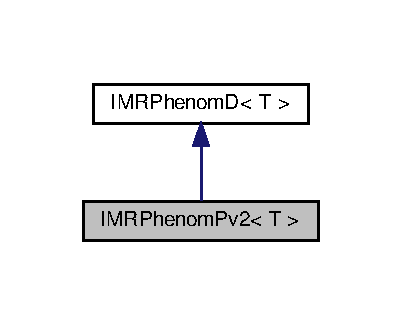
\includegraphics[width=252pt]{classIMRPhenomPv2__inherit__graph}
\end{center}
\end{figure}


Collaboration diagram for I\+M\+R\+Phenom\+Pv2$<$ T $>$\+:
\nopagebreak
\begin{figure}[H]
\begin{center}
\leavevmode
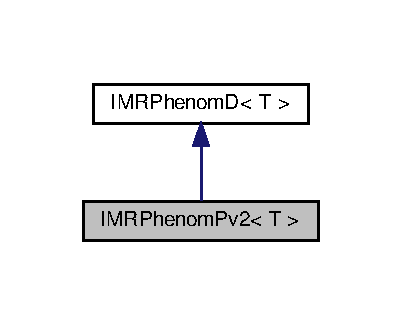
\includegraphics[width=193pt]{classIMRPhenomPv2__coll__graph}
\end{center}
\end{figure}
\doxysubsection*{Public Member Functions}
\begin{DoxyCompactItemize}
\item 
\mbox{\Hypertarget{classIMRPhenomPv2_ae3a484c9f30a94cde0fd996e164e1f7d}\label{classIMRPhenomPv2_ae3a484c9f30a94cde0fd996e164e1f7d}} 
virtual T {\bfseries alpha} (T omega, T q, T chi2l, T chi2)
\item 
\mbox{\Hypertarget{classIMRPhenomPv2_a5fff973809492fa59aff6d7d44a2b37a}\label{classIMRPhenomPv2_a5fff973809492fa59aff6d7d44a2b37a}} 
virtual T {\bfseries epsilon} (T omega, T q, T chi2l, T chi2)
\item 
virtual void \mbox{\hyperlink{classIMRPhenomPv2_afc0f88c773f46ab060482bc530f60115}{calculate\+\_\+euler\+\_\+coeffs}} (\mbox{\hyperlink{structalpha__coeffs}{alpha\+\_\+coeffs}}$<$ T $>$ $\ast$acoeffs, \mbox{\hyperlink{structepsilon__coeffs}{epsilon\+\_\+coeffs}}$<$ T $>$ $\ast$ecoeffs, \mbox{\hyperlink{structsource__parameters}{source\+\_\+parameters}}$<$ T $>$ $\ast$params)
\begin{DoxyCompactList}\small\item\em Pre calculate euler angle coefficients. \end{DoxyCompactList}\item 
\mbox{\Hypertarget{classIMRPhenomPv2_a61b485a13745066477875a4b192dd940}\label{classIMRPhenomPv2_a61b485a13745066477875a4b192dd940}} 
virtual T {\bfseries d} (int l, int mp, int m, T s)
\item 
virtual void \mbox{\hyperlink{classIMRPhenomPv2_a9c81435792ee35948b3e7b3438c1ef1e}{Phenom\+Pv2\+\_\+\+J\+S\+F\+\_\+from\+\_\+params}} (\mbox{\hyperlink{classgen__params__base}{gen\+\_\+params\+\_\+base}}$<$ T $>$ $\ast$params, T $\ast$J\+SF)
\begin{DoxyCompactList}\small\item\em Calculate the unit vector in the direction of the total angular momentum. \end{DoxyCompactList}\item 
virtual int \mbox{\hyperlink{classIMRPhenomPv2_af147bf8756311a9386b3f9bcdefa7dd5}{construct\+\_\+waveform}} (T $\ast$frequencies, int length, std\+::complex$<$ T $>$ $\ast$waveform\+\_\+plus, std\+::complex$<$ T $>$ $\ast$waveform\+\_\+cross, \mbox{\hyperlink{structsource__parameters}{source\+\_\+parameters}}$<$ T $>$ $\ast$params)
\begin{DoxyCompactList}\small\item\em Constructs the waveform for \mbox{\hyperlink{classIMRPhenomPv2}{I\+M\+R\+Phenom\+Pv2}} -\/ uses \mbox{\hyperlink{classIMRPhenomD}{I\+M\+R\+PhenomD}}, then twists up. \end{DoxyCompactList}\item 
virtual int \mbox{\hyperlink{classIMRPhenomPv2_a05877c187dedd47f2479939907b4b2e9}{construct\+\_\+phase}} (T $\ast$frequencies, int length, T $\ast$phase\+\_\+plus, T $\ast$phase\+\_\+cross, \mbox{\hyperlink{structsource__parameters}{source\+\_\+parameters}}$<$ T $>$ $\ast$params)
\begin{DoxyCompactList}\small\item\em Constructs the phase for \mbox{\hyperlink{classIMRPhenomPv2}{I\+M\+R\+Phenom\+Pv2}} -\/ uses \mbox{\hyperlink{classIMRPhenomD}{I\+M\+R\+PhenomD}}, then twists up. \end{DoxyCompactList}\item 
\mbox{\Hypertarget{classIMRPhenomPv2_a326eaa63c365113abfa37830f0a0f42f}\label{classIMRPhenomPv2_a326eaa63c365113abfa37830f0a0f42f}} 
virtual T {\bfseries calculate\+\_\+time\+\_\+shift} (\mbox{\hyperlink{structsource__parameters}{source\+\_\+parameters}}$<$ T $>$ $\ast$params, \mbox{\hyperlink{structuseful__powers}{useful\+\_\+powers}}$<$ T $>$ $\ast$pows, T $\ast$pn\+\_\+phase\+\_\+coeffs, \mbox{\hyperlink{structlambda__parameters}{lambda\+\_\+parameters}}$<$ T $>$ $\ast$lambda)
\item 
\mbox{\Hypertarget{classIMRPhenomPv2_abd66fb1738b26466d28d8f4050d4207c}\label{classIMRPhenomPv2_abd66fb1738b26466d28d8f4050d4207c}} 
virtual void {\bfseries WignerD} (T d2\mbox{[}5\mbox{]}, T dm2\mbox{[}5\mbox{]}, \mbox{\hyperlink{structuseful__powers}{useful\+\_\+powers}}$<$ T $>$ $\ast$pows, \mbox{\hyperlink{structsource__parameters}{source\+\_\+parameters}}$<$ T $>$ $\ast$params)
\item 
\mbox{\Hypertarget{classIMRPhenomPv2_a2f7dc5cbc5451036e15b7eaa3e170f96}\label{classIMRPhenomPv2_a2f7dc5cbc5451036e15b7eaa3e170f96}} 
virtual void {\bfseries calculate\+\_\+twistup} (T alpha, std\+::complex$<$ T $>$ $\ast$hp\+\_\+factor, std\+::complex$<$ T $>$ $\ast$hc\+\_\+factor, T d2\mbox{[}5\mbox{]}, T dm2\mbox{[}5\mbox{]}, \mbox{\hyperlink{structsph__harm}{sph\+\_\+harm}}$<$ T $>$ $\ast$\mbox{\hyperlink{structsph__harm}{sph\+\_\+harm}})
\item 
\mbox{\Hypertarget{classIMRPhenomPv2_aba929d7ceebe4ddbfd13088c1ac0596b}\label{classIMRPhenomPv2_aba929d7ceebe4ddbfd13088c1ac0596b}} 
virtual void {\bfseries calculate\+\_\+euler\+\_\+angles} (T $\ast$alpha, T $\ast$epsilon, \mbox{\hyperlink{structuseful__powers}{useful\+\_\+powers}}$<$ T $>$ $\ast$pows, \mbox{\hyperlink{structalpha__coeffs}{alpha\+\_\+coeffs}}$<$ T $>$ $\ast$acoeffs, \mbox{\hyperlink{structepsilon__coeffs}{epsilon\+\_\+coeffs}}$<$ T $>$ $\ast$ecoeffs)
\item 
virtual void \mbox{\hyperlink{classIMRPhenomPv2_ae8f253a1feebc43995dd5d052c856e05}{Phenom\+Pv2\+\_\+\+Param\+\_\+\+Transform}} (\mbox{\hyperlink{structsource__parameters}{source\+\_\+parameters}}$<$ T $>$ $\ast$params)
\item 
virtual void \mbox{\hyperlink{classIMRPhenomPv2_a684f1bbc22773a72e8000de61c1b6def}{Phenom\+Pv2\+\_\+\+Param\+\_\+\+Transform\+\_\+J}} (\mbox{\hyperlink{structsource__parameters}{source\+\_\+parameters}}$<$ T $>$ $\ast$params)
\item 
virtual void \mbox{\hyperlink{classIMRPhenomPv2_a09917aef3521bd8e3b8d8516930077a0}{Phenom\+Pv2\+\_\+\+Param\+\_\+\+Transform\+\_\+reduced}} (\mbox{\hyperlink{structsource__parameters}{source\+\_\+parameters}}$<$ T $>$ $\ast$params)
\item 
\mbox{\Hypertarget{classIMRPhenomPv2_a5e64520f828d29beccdf5b1e5e18582c}\label{classIMRPhenomPv2_a5e64520f828d29beccdf5b1e5e18582c}} 
virtual T {\bfseries L2\+PN} (T eta, \mbox{\hyperlink{structuseful__powers}{useful\+\_\+powers}}$<$ T $>$ $\ast$pow)
\item 
virtual T \mbox{\hyperlink{classIMRPhenomPv2_a36cbd07ab5b8c1663c7f8c8e75cf4e74}{Final\+Spin\+I\+M\+R\+Phenom\+D\+\_\+all\+\_\+in\+\_\+plane\+\_\+spin\+\_\+on\+\_\+larger\+\_\+\+BH}} (T m1, T m2, T chi1\+\_\+l, T chi2\+\_\+l, T chip)
\item 
\mbox{\Hypertarget{classIMRPhenomPv2_a3d37a40e4d1bce6ca673e6b30e64fe67}\label{classIMRPhenomPv2_a3d37a40e4d1bce6ca673e6b30e64fe67}} 
virtual T {\bfseries final\+\_\+spin} (\mbox{\hyperlink{structsource__parameters}{source\+\_\+parameters}}$<$ T $>$ $\ast$params)
\item 
{\footnotesize template$<$$>$ }\\double \mbox{\hyperlink{classIMRPhenomPv2_a6b27bd676726358b699a35cfbd10fe79}{calculate\+\_\+time\+\_\+shift}} (\mbox{\hyperlink{structsource__parameters}{source\+\_\+parameters}}$<$ double $>$ $\ast$params, \mbox{\hyperlink{structuseful__powers}{useful\+\_\+powers}}$<$ double $>$ $\ast$pows, double $\ast$pn\+\_\+phase\+\_\+coeffs, \mbox{\hyperlink{structlambda__parameters}{lambda\+\_\+parameters}}$<$ double $>$ $\ast$lambda)
\begin{DoxyCompactList}\small\item\em Shifts the time of coalescence to the desired value. \end{DoxyCompactList}\item 
{\footnotesize template$<$$>$ }\\adouble \mbox{\hyperlink{classIMRPhenomPv2_a61ec2bf7f72ec82b5a583e7098b2daab}{calculate\+\_\+time\+\_\+shift}} (\mbox{\hyperlink{structsource__parameters}{source\+\_\+parameters}}$<$ adouble $>$ $\ast$params, \mbox{\hyperlink{structuseful__powers}{useful\+\_\+powers}}$<$ adouble $>$ $\ast$pows, adouble $\ast$pn\+\_\+phase\+\_\+coeffs, \mbox{\hyperlink{structlambda__parameters}{lambda\+\_\+parameters}}$<$ adouble $>$ $\ast$lambda)
\begin{DoxyCompactList}\small\item\em Shifts the time of coalescence to the desired value. \end{DoxyCompactList}\end{DoxyCompactItemize}


\doxysubsection{Member Function Documentation}
\mbox{\Hypertarget{classIMRPhenomPv2_afc0f88c773f46ab060482bc530f60115}\label{classIMRPhenomPv2_afc0f88c773f46ab060482bc530f60115}} 
\index{IMRPhenomPv2$<$ T $>$@{IMRPhenomPv2$<$ T $>$}!calculate\_euler\_coeffs@{calculate\_euler\_coeffs}}
\index{calculate\_euler\_coeffs@{calculate\_euler\_coeffs}!IMRPhenomPv2$<$ T $>$@{IMRPhenomPv2$<$ T $>$}}
\doxysubsubsection{\texorpdfstring{calculate\_euler\_coeffs()}{calculate\_euler\_coeffs()}}
{\footnotesize\ttfamily template$<$class T $>$ \\
void \mbox{\hyperlink{classIMRPhenomPv2}{I\+M\+R\+Phenom\+Pv2}}$<$ T $>$\+::calculate\+\_\+euler\+\_\+coeffs (\begin{DoxyParamCaption}\item[{\mbox{\hyperlink{structalpha__coeffs}{alpha\+\_\+coeffs}}$<$ T $>$ $\ast$}]{acoeffs,  }\item[{\mbox{\hyperlink{structepsilon__coeffs}{epsilon\+\_\+coeffs}}$<$ T $>$ $\ast$}]{ecoeffs,  }\item[{\mbox{\hyperlink{structsource__parameters}{source\+\_\+parameters}}$<$ T $>$ $\ast$}]{params }\end{DoxyParamCaption})\hspace{0.3cm}{\ttfamily [virtual]}}



Pre calculate euler angle coefficients. 

Straight up stolen from L\+A\+Lsuite \mbox{\Hypertarget{classIMRPhenomPv2_a61ec2bf7f72ec82b5a583e7098b2daab}\label{classIMRPhenomPv2_a61ec2bf7f72ec82b5a583e7098b2daab}} 
\index{IMRPhenomPv2$<$ T $>$@{IMRPhenomPv2$<$ T $>$}!calculate\_time\_shift@{calculate\_time\_shift}}
\index{calculate\_time\_shift@{calculate\_time\_shift}!IMRPhenomPv2$<$ T $>$@{IMRPhenomPv2$<$ T $>$}}
\doxysubsubsection{\texorpdfstring{calculate\_time\_shift()}{calculate\_time\_shift()}\hspace{0.1cm}{\footnotesize\ttfamily [1/2]}}
{\footnotesize\ttfamily template$<$$>$ \\
adouble \mbox{\hyperlink{classIMRPhenomPv2}{I\+M\+R\+Phenom\+Pv2}}$<$ adouble $>$\+::calculate\+\_\+time\+\_\+shift (\begin{DoxyParamCaption}\item[{\mbox{\hyperlink{structsource__parameters}{source\+\_\+parameters}}$<$ adouble $>$ $\ast$}]{params,  }\item[{\mbox{\hyperlink{structuseful__powers}{useful\+\_\+powers}}$<$ adouble $>$ $\ast$}]{pows,  }\item[{adouble $\ast$}]{pn\+\_\+phase\+\_\+coeffs,  }\item[{\mbox{\hyperlink{structlambda__parameters}{lambda\+\_\+parameters}}$<$ adouble $>$ $\ast$}]{lambda }\end{DoxyParamCaption})}



Shifts the time of coalescence to the desired value. 

Because G\+SL interpolation must have double (not adouble), the two cases must behandled separately, explicitly. \mbox{\Hypertarget{classIMRPhenomPv2_a6b27bd676726358b699a35cfbd10fe79}\label{classIMRPhenomPv2_a6b27bd676726358b699a35cfbd10fe79}} 
\index{IMRPhenomPv2$<$ T $>$@{IMRPhenomPv2$<$ T $>$}!calculate\_time\_shift@{calculate\_time\_shift}}
\index{calculate\_time\_shift@{calculate\_time\_shift}!IMRPhenomPv2$<$ T $>$@{IMRPhenomPv2$<$ T $>$}}
\doxysubsubsection{\texorpdfstring{calculate\_time\_shift()}{calculate\_time\_shift()}\hspace{0.1cm}{\footnotesize\ttfamily [2/2]}}
{\footnotesize\ttfamily template$<$$>$ \\
double \mbox{\hyperlink{classIMRPhenomPv2}{I\+M\+R\+Phenom\+Pv2}}$<$ double $>$\+::calculate\+\_\+time\+\_\+shift (\begin{DoxyParamCaption}\item[{\mbox{\hyperlink{structsource__parameters}{source\+\_\+parameters}}$<$ double $>$ $\ast$}]{params,  }\item[{\mbox{\hyperlink{structuseful__powers}{useful\+\_\+powers}}$<$ double $>$ $\ast$}]{pows,  }\item[{double $\ast$}]{pn\+\_\+phase\+\_\+coeffs,  }\item[{\mbox{\hyperlink{structlambda__parameters}{lambda\+\_\+parameters}}$<$ double $>$ $\ast$}]{lambda }\end{DoxyParamCaption})}



Shifts the time of coalescence to the desired value. 

Because G\+SL interpolation must have double (not adouble), the two cases must behandled separately, explicitly. \mbox{\Hypertarget{classIMRPhenomPv2_a05877c187dedd47f2479939907b4b2e9}\label{classIMRPhenomPv2_a05877c187dedd47f2479939907b4b2e9}} 
\index{IMRPhenomPv2$<$ T $>$@{IMRPhenomPv2$<$ T $>$}!construct\_phase@{construct\_phase}}
\index{construct\_phase@{construct\_phase}!IMRPhenomPv2$<$ T $>$@{IMRPhenomPv2$<$ T $>$}}
\doxysubsubsection{\texorpdfstring{construct\_phase()}{construct\_phase()}}
{\footnotesize\ttfamily template$<$class T $>$ \\
int \mbox{\hyperlink{classIMRPhenomPv2}{I\+M\+R\+Phenom\+Pv2}}$<$ T $>$\+::construct\+\_\+phase (\begin{DoxyParamCaption}\item[{T $\ast$}]{frequencies,  }\item[{int}]{length,  }\item[{T $\ast$}]{phase\+\_\+plus,  }\item[{T $\ast$}]{phase\+\_\+cross,  }\item[{\mbox{\hyperlink{structsource__parameters}{source\+\_\+parameters}}$<$ T $>$ $\ast$}]{params }\end{DoxyParamCaption})\hspace{0.3cm}{\ttfamily [virtual]}}



Constructs the phase for \mbox{\hyperlink{classIMRPhenomPv2}{I\+M\+R\+Phenom\+Pv2}} -\/ uses \mbox{\hyperlink{classIMRPhenomD}{I\+M\+R\+PhenomD}}, then twists up. 

arguments\+: array of frequencies, length of that array, a complex array for the output waveform, and a \mbox{\hyperlink{structsource__parameters}{source\+\_\+parameters}} structure 
\begin{DoxyParams}{Parameters}
{\em frequencies} & T array of frequencies the waveform is to be evaluated at \\
\hline
{\em length} & integer length of the array of frequencies and the waveform \\
\hline
{\em phase\+\_\+plus} & complex T array for the plus polariaztion waveform to be output \\
\hline
{\em phase\+\_\+cross} & complex T array for the cross polarization waveform to be output \\
\hline
\end{DoxyParams}
\mbox{\Hypertarget{classIMRPhenomPv2_af147bf8756311a9386b3f9bcdefa7dd5}\label{classIMRPhenomPv2_af147bf8756311a9386b3f9bcdefa7dd5}} 
\index{IMRPhenomPv2$<$ T $>$@{IMRPhenomPv2$<$ T $>$}!construct\_waveform@{construct\_waveform}}
\index{construct\_waveform@{construct\_waveform}!IMRPhenomPv2$<$ T $>$@{IMRPhenomPv2$<$ T $>$}}
\doxysubsubsection{\texorpdfstring{construct\_waveform()}{construct\_waveform()}}
{\footnotesize\ttfamily template$<$class T $>$ \\
int \mbox{\hyperlink{classIMRPhenomPv2}{I\+M\+R\+Phenom\+Pv2}}$<$ T $>$\+::construct\+\_\+waveform (\begin{DoxyParamCaption}\item[{T $\ast$}]{frequencies,  }\item[{int}]{length,  }\item[{std\+::complex$<$ T $>$ $\ast$}]{waveform\+\_\+plus,  }\item[{std\+::complex$<$ T $>$ $\ast$}]{waveform\+\_\+cross,  }\item[{\mbox{\hyperlink{structsource__parameters}{source\+\_\+parameters}}$<$ T $>$ $\ast$}]{params }\end{DoxyParamCaption})\hspace{0.3cm}{\ttfamily [virtual]}}



Constructs the waveform for \mbox{\hyperlink{classIMRPhenomPv2}{I\+M\+R\+Phenom\+Pv2}} -\/ uses \mbox{\hyperlink{classIMRPhenomD}{I\+M\+R\+PhenomD}}, then twists up. 

arguments\+: array of frequencies, length of that array, a complex array for the output waveform, and a \mbox{\hyperlink{structsource__parameters}{source\+\_\+parameters}} structure 
\begin{DoxyParams}{Parameters}
{\em frequencies} & T array of frequencies the waveform is to be evaluated at \\
\hline
{\em length} & integer length of the array of frequencies and the waveform \\
\hline
{\em waveform\+\_\+plus} & complex T array for the plus polariaztion waveform to be output \\
\hline
{\em waveform\+\_\+cross} & complex T array for the cross polarization waveform to be output \\
\hline
\end{DoxyParams}
\mbox{\Hypertarget{classIMRPhenomPv2_a36cbd07ab5b8c1663c7f8c8e75cf4e74}\label{classIMRPhenomPv2_a36cbd07ab5b8c1663c7f8c8e75cf4e74}} 
\index{IMRPhenomPv2$<$ T $>$@{IMRPhenomPv2$<$ T $>$}!FinalSpinIMRPhenomD\_all\_in\_plane\_spin\_on\_larger\_BH@{FinalSpinIMRPhenomD\_all\_in\_plane\_spin\_on\_larger\_BH}}
\index{FinalSpinIMRPhenomD\_all\_in\_plane\_spin\_on\_larger\_BH@{FinalSpinIMRPhenomD\_all\_in\_plane\_spin\_on\_larger\_BH}!IMRPhenomPv2$<$ T $>$@{IMRPhenomPv2$<$ T $>$}}
\doxysubsubsection{\texorpdfstring{FinalSpinIMRPhenomD\_all\_in\_plane\_spin\_on\_larger\_BH()}{FinalSpinIMRPhenomD\_all\_in\_plane\_spin\_on\_larger\_BH()}}
{\footnotesize\ttfamily template$<$class T $>$ \\
T \mbox{\hyperlink{classIMRPhenomPv2}{I\+M\+R\+Phenom\+Pv2}}$<$ T $>$\+::Final\+Spin\+I\+M\+R\+Phenom\+D\+\_\+all\+\_\+in\+\_\+plane\+\_\+spin\+\_\+on\+\_\+larger\+\_\+\+BH (\begin{DoxyParamCaption}\item[{T}]{m1,  }\item[{T}]{m2,  }\item[{T}]{chi1\+\_\+l,  }\item[{T}]{chi2\+\_\+l,  }\item[{T}]{chip }\end{DoxyParamCaption})\hspace{0.3cm}{\ttfamily [virtual]}}


\begin{DoxyItemize}
\item Wrapper for final-\/spin formula based on\+:
\begin{DoxyItemize}
\item -\/ \mbox{\hyperlink{classIMRPhenomD}{I\+M\+R\+PhenomD}}\textquotesingle{}s \mbox{\hyperlink{classIMRPhenomD_af638fe3433f2367f9dfe6e2236a6b0ee}{Final\+Spin0815()}} for aligned spins.
\begin{DoxyItemize}
\item 
\begin{DoxyItemize}
\item We use their convention m1$>$m2
\begin{DoxyItemize}
\item and put {\bfseries{all in-\/plane spin on the larger BH}}.
\begin{DoxyItemize}
\item 
\begin{DoxyItemize}
\item In the aligned limit return the Final\+Spin0815 value. 
\end{DoxyItemize}
\end{DoxyItemize}
\end{DoxyItemize}
\end{DoxyItemize}
\end{DoxyItemize}
\end{DoxyItemize}
\end{DoxyItemize}
\begin{DoxyParams}{Parameters}
{\em m1} & Mass of companion 1 (solar masses) \\
\hline
{\em m2} & Mass of companion 2 (solar masses) \\
\hline
{\em chi1\+\_\+l} & Aligned spin of BH 1 \\
\hline
{\em chi2\+\_\+l} & Aligned spin of BH 2 \\
\hline
{\em chip} & Dimensionless spin in the orbital plane \\
\hline
\end{DoxyParams}
\mbox{\Hypertarget{classIMRPhenomPv2_a9c81435792ee35948b3e7b3438c1ef1e}\label{classIMRPhenomPv2_a9c81435792ee35948b3e7b3438c1ef1e}} 
\index{IMRPhenomPv2$<$ T $>$@{IMRPhenomPv2$<$ T $>$}!PhenomPv2\_JSF\_from\_params@{PhenomPv2\_JSF\_from\_params}}
\index{PhenomPv2\_JSF\_from\_params@{PhenomPv2\_JSF\_from\_params}!IMRPhenomPv2$<$ T $>$@{IMRPhenomPv2$<$ T $>$}}
\doxysubsubsection{\texorpdfstring{PhenomPv2\_JSF\_from\_params()}{PhenomPv2\_JSF\_from\_params()}}
{\footnotesize\ttfamily template$<$class T $>$ \\
void \mbox{\hyperlink{classIMRPhenomPv2}{I\+M\+R\+Phenom\+Pv2}}$<$ T $>$\+::Phenom\+Pv2\+\_\+\+J\+S\+F\+\_\+from\+\_\+params (\begin{DoxyParamCaption}\item[{\mbox{\hyperlink{classgen__params__base}{gen\+\_\+params\+\_\+base}}$<$ T $>$ $\ast$}]{params,  }\item[{T $\ast$}]{J\+SF }\end{DoxyParamCaption})\hspace{0.3cm}{\ttfamily [virtual]}}



Calculate the unit vector in the direction of the total angular momentum. 

\mbox{\Hypertarget{classIMRPhenomPv2_ae8f253a1feebc43995dd5d052c856e05}\label{classIMRPhenomPv2_ae8f253a1feebc43995dd5d052c856e05}} 
\index{IMRPhenomPv2$<$ T $>$@{IMRPhenomPv2$<$ T $>$}!PhenomPv2\_Param\_Transform@{PhenomPv2\_Param\_Transform}}
\index{PhenomPv2\_Param\_Transform@{PhenomPv2\_Param\_Transform}!IMRPhenomPv2$<$ T $>$@{IMRPhenomPv2$<$ T $>$}}
\doxysubsubsection{\texorpdfstring{PhenomPv2\_Param\_Transform()}{PhenomPv2\_Param\_Transform()}}
{\footnotesize\ttfamily template$<$class T $>$ \\
void \mbox{\hyperlink{classIMRPhenomPv2}{I\+M\+R\+Phenom\+Pv2}}$<$ T $>$\+::Phenom\+Pv2\+\_\+\+Param\+\_\+\+Transform (\begin{DoxyParamCaption}\item[{\mbox{\hyperlink{structsource__parameters}{source\+\_\+parameters}}$<$ T $>$ $\ast$}]{params }\end{DoxyParamCaption})\hspace{0.3cm}{\ttfamily [virtual]}}

/\+Brief Parameter transformtion to precalculate needed parameters for PhenomP from source parameters

Pretty much stolen verbatim from lalsuite \mbox{\Hypertarget{classIMRPhenomPv2_a684f1bbc22773a72e8000de61c1b6def}\label{classIMRPhenomPv2_a684f1bbc22773a72e8000de61c1b6def}} 
\index{IMRPhenomPv2$<$ T $>$@{IMRPhenomPv2$<$ T $>$}!PhenomPv2\_Param\_Transform\_J@{PhenomPv2\_Param\_Transform\_J}}
\index{PhenomPv2\_Param\_Transform\_J@{PhenomPv2\_Param\_Transform\_J}!IMRPhenomPv2$<$ T $>$@{IMRPhenomPv2$<$ T $>$}}
\doxysubsubsection{\texorpdfstring{PhenomPv2\_Param\_Transform\_J()}{PhenomPv2\_Param\_Transform\_J()}}
{\footnotesize\ttfamily template$<$class T $>$ \\
void \mbox{\hyperlink{classIMRPhenomPv2}{I\+M\+R\+Phenom\+Pv2}}$<$ T $>$\+::Phenom\+Pv2\+\_\+\+Param\+\_\+\+Transform\+\_\+J (\begin{DoxyParamCaption}\item[{\mbox{\hyperlink{structsource__parameters}{source\+\_\+parameters}}$<$ T $>$ $\ast$}]{params }\end{DoxyParamCaption})\hspace{0.3cm}{\ttfamily [virtual]}}

/\+Brief Parameter transformtion to precalculate needed parameters for PhenomP from source parameters -- assumed inclination of total angular momentum J is given, not orbital angular momentum (in source frame (Lhat == zhat)

Pretty much stolen verbatim from lalsuite \mbox{\Hypertarget{classIMRPhenomPv2_a09917aef3521bd8e3b8d8516930077a0}\label{classIMRPhenomPv2_a09917aef3521bd8e3b8d8516930077a0}} 
\index{IMRPhenomPv2$<$ T $>$@{IMRPhenomPv2$<$ T $>$}!PhenomPv2\_Param\_Transform\_reduced@{PhenomPv2\_Param\_Transform\_reduced}}
\index{PhenomPv2\_Param\_Transform\_reduced@{PhenomPv2\_Param\_Transform\_reduced}!IMRPhenomPv2$<$ T $>$@{IMRPhenomPv2$<$ T $>$}}
\doxysubsubsection{\texorpdfstring{PhenomPv2\_Param\_Transform\_reduced()}{PhenomPv2\_Param\_Transform\_reduced()}}
{\footnotesize\ttfamily template$<$class T $>$ \\
void \mbox{\hyperlink{classIMRPhenomPv2}{I\+M\+R\+Phenom\+Pv2}}$<$ T $>$\+::Phenom\+Pv2\+\_\+\+Param\+\_\+\+Transform\+\_\+reduced (\begin{DoxyParamCaption}\item[{\mbox{\hyperlink{structsource__parameters}{source\+\_\+parameters}}$<$ T $>$ $\ast$}]{params }\end{DoxyParamCaption})\hspace{0.3cm}{\ttfamily [virtual]}}

/\+Brief Parameter transformation to pre-\/calculate needed parameters for PhenomP from source parameters

Pretty much stolen verbatim from lalsuite 

The documentation for this class was generated from the following files\+:\begin{DoxyCompactItemize}
\item 
include/gwat/\mbox{\hyperlink{IMRPhenomP_8h}{I\+M\+R\+Phenom\+P.\+h}}\item 
src/\mbox{\hyperlink{IMRPhenomP_8cpp}{I\+M\+R\+Phenom\+P.\+cpp}}\end{DoxyCompactItemize}

\hypertarget{structlambda__parameters}{}\section{lambda\+\_\+parameters$<$ T $>$ Struct Template Reference}
\label{structlambda__parameters}\index{lambda\+\_\+parameters$<$ T $>$@{lambda\+\_\+parameters$<$ T $>$}}


Collaboration diagram for lambda\+\_\+parameters$<$ T $>$\+:\nopagebreak
\begin{figure}[H]
\begin{center}
\leavevmode
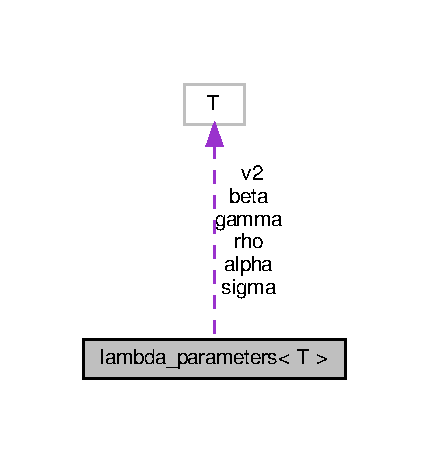
\includegraphics[width=206pt]{structlambda__parameters__coll__graph}
\end{center}
\end{figure}
\subsection*{Public Attributes}
\begin{DoxyCompactItemize}
\item 
\mbox{\Hypertarget{structlambda__parameters_a08f293753fe41b88fdd8a206b593a6c8}\label{structlambda__parameters_a08f293753fe41b88fdd8a206b593a6c8}} 
T {\bfseries rho} \mbox{[}4\mbox{]}
\item 
\mbox{\Hypertarget{structlambda__parameters_a35ec87e1f27de9393a6e94d18cd63c52}\label{structlambda__parameters_a35ec87e1f27de9393a6e94d18cd63c52}} 
T {\bfseries v2}
\item 
\mbox{\Hypertarget{structlambda__parameters_a49db18626c20bd43f25c5c760679ac2a}\label{structlambda__parameters_a49db18626c20bd43f25c5c760679ac2a}} 
T {\bfseries gamma} \mbox{[}4\mbox{]}
\item 
\mbox{\Hypertarget{structlambda__parameters_aefdccc025bcb819ec4b8009b232cf9b2}\label{structlambda__parameters_aefdccc025bcb819ec4b8009b232cf9b2}} 
T {\bfseries sigma} \mbox{[}5\mbox{]}
\item 
\mbox{\Hypertarget{structlambda__parameters_a4aa387f5a44b09541304c5e2f8f3aad6}\label{structlambda__parameters_a4aa387f5a44b09541304c5e2f8f3aad6}} 
T {\bfseries beta} \mbox{[}5\mbox{]}
\item 
\mbox{\Hypertarget{structlambda__parameters_aec862d891bc928fb1faf042aff322802}\label{structlambda__parameters_aec862d891bc928fb1faf042aff322802}} 
T {\bfseries alpha} \mbox{[}7\mbox{]}
\end{DoxyCompactItemize}


The documentation for this struct was generated from the following file\+:\begin{DoxyCompactItemize}
\item 
include/gwat/\hyperlink{IMRPhenomD_8h}{I\+M\+R\+Phenom\+D.\+h}\end{DoxyCompactItemize}

\hypertarget{classppE__IMRPhenomD__IMR}{}\doxysection{pp\+E\+\_\+\+I\+M\+R\+Phenom\+D\+\_\+\+I\+MR$<$ T $>$ Class Template Reference}
\label{classppE__IMRPhenomD__IMR}\index{ppE\_IMRPhenomD\_IMR$<$ T $>$@{ppE\_IMRPhenomD\_IMR$<$ T $>$}}


{\ttfamily \#include $<$pp\+E\+\_\+\+I\+M\+R\+Phenom\+D.\+h$>$}



Inheritance diagram for pp\+E\+\_\+\+I\+M\+R\+Phenom\+D\+\_\+\+I\+MR$<$ T $>$\+:
\nopagebreak
\begin{figure}[H]
\begin{center}
\leavevmode
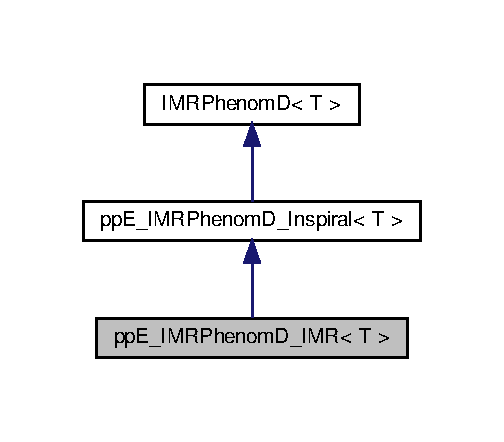
\includegraphics[width=242pt]{classppE__IMRPhenomD__IMR__inherit__graph}
\end{center}
\end{figure}


Collaboration diagram for pp\+E\+\_\+\+I\+M\+R\+Phenom\+D\+\_\+\+I\+MR$<$ T $>$\+:
\nopagebreak
\begin{figure}[H]
\begin{center}
\leavevmode
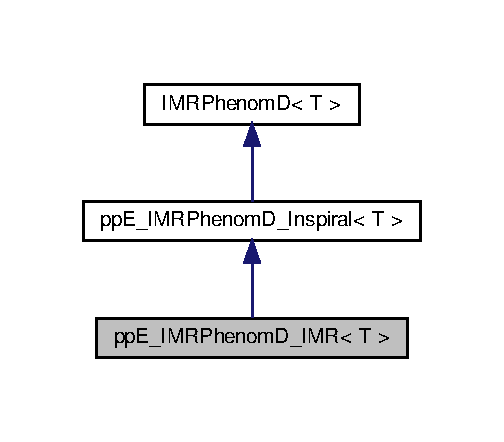
\includegraphics[width=242pt]{classppE__IMRPhenomD__IMR__coll__graph}
\end{center}
\end{figure}
\doxysubsection*{Public Member Functions}
\begin{DoxyCompactItemize}
\item 
virtual T \mbox{\hyperlink{classppE__IMRPhenomD__IMR_a3fa643eca535e7bef26f70bd5ed4cbde}{Dphase\+\_\+mr}} (T f, \mbox{\hyperlink{structsource__parameters}{source\+\_\+parameters}}$<$ T $>$ $\ast$param, \mbox{\hyperlink{structlambda__parameters}{lambda\+\_\+parameters}}$<$ T $>$ $\ast$lambda)
\begin{DoxyCompactList}\small\item\em Calculates the derivative of the merger-\/ringdown phase for frequency f. \end{DoxyCompactList}\item 
virtual T \mbox{\hyperlink{classppE__IMRPhenomD__IMR_a3b64e9bbf566450687bcfaa85c0e493f}{phase\+\_\+mr}} (T f, \mbox{\hyperlink{structsource__parameters}{source\+\_\+parameters}}$<$ T $>$ $\ast$param, \mbox{\hyperlink{structlambda__parameters}{lambda\+\_\+parameters}}$<$ T $>$ $\ast$lambda)
\begin{DoxyCompactList}\small\item\em Calculates the merger-\/ringdown phase for frequency f. \end{DoxyCompactList}\item 
virtual T \mbox{\hyperlink{classppE__IMRPhenomD__IMR_a04dc31c54da6e199db28197665b469a1}{phase\+\_\+int}} (T f, \mbox{\hyperlink{structsource__parameters}{source\+\_\+parameters}}$<$ T $>$ $\ast$param, \mbox{\hyperlink{structlambda__parameters}{lambda\+\_\+parameters}}$<$ T $>$ $\ast$lambda)
\begin{DoxyCompactList}\small\item\em Calculates the intermediate phase for frequency f. \end{DoxyCompactList}\item 
virtual T \mbox{\hyperlink{classppE__IMRPhenomD__IMR_a1625961885f0bf0723d1c12818cca287}{Dphase\+\_\+int}} (T f, \mbox{\hyperlink{structsource__parameters}{source\+\_\+parameters}}$<$ T $>$ $\ast$param, \mbox{\hyperlink{structlambda__parameters}{lambda\+\_\+parameters}}$<$ T $>$ $\ast$lambda)
\begin{DoxyCompactList}\small\item\em Calculates the derivative of the intermediate phase for frequency f. \end{DoxyCompactList}\item 
\mbox{\Hypertarget{classppE__IMRPhenomD__IMR_a698b02b83bfbc22e5ebc0e2e4f2f82fe}\label{classppE__IMRPhenomD__IMR_a698b02b83bfbc22e5ebc0e2e4f2f82fe}} 
virtual void {\bfseries fisher\+\_\+calculation\+\_\+sky\+\_\+averaged} (double $\ast$frequency, int length, \mbox{\hyperlink{classgen__params}{gen\+\_\+params}} $\ast$parameters, double $\ast$$\ast$amplitude\+\_\+deriv, double $\ast$$\ast$phase\+\_\+deriv, double $\ast$amplitude, int $\ast$amp\+\_\+tapes, int $\ast$phase\+\_\+tapes)
\item 
virtual void \mbox{\hyperlink{classppE__IMRPhenomD__IMR_a3119a07c11ed53ae94823b11c5234c4f}{amplitude\+\_\+tape}} (\mbox{\hyperlink{structsource__parameters}{source\+\_\+parameters}}$<$ double $>$ $\ast$input\+\_\+params, int $\ast$tape)
\begin{DoxyCompactList}\small\item\em Creates the tapes for derivatives of the amplitude. \end{DoxyCompactList}\item 
virtual void \mbox{\hyperlink{classppE__IMRPhenomD__IMR_acf2ed8617b3e24ecc273a409ff579ce4}{phase\+\_\+tape}} (\mbox{\hyperlink{structsource__parameters}{source\+\_\+parameters}}$<$ double $>$ $\ast$input\+\_\+params, int $\ast$tape)
\begin{DoxyCompactList}\small\item\em Creates the tapes for derivatives of phase. \end{DoxyCompactList}\item 
virtual void \mbox{\hyperlink{classppE__IMRPhenomD__IMR_a5b80e5ae4dd83da49beb15e6e5f17715}{construct\+\_\+amplitude\+\_\+derivative}} (double $\ast$frequencies, int length, int dimension, double $\ast$$\ast$amplitude\+\_\+derivative, \mbox{\hyperlink{structsource__parameters}{source\+\_\+parameters}}$<$ double $>$ $\ast$input\+\_\+params, int $\ast$tapes=N\+U\+LL)
\begin{DoxyCompactList}\small\item\em Construct the derivative of the amplitude for a given source evaluated by the given frequency. \end{DoxyCompactList}\item 
virtual void \mbox{\hyperlink{classppE__IMRPhenomD__IMR_a78151d1f34693b69cf6ccbc28df4caa6}{construct\+\_\+phase\+\_\+derivative}} (double $\ast$frequencies, int length, int dimension, double $\ast$$\ast$phase\+\_\+derivative, \mbox{\hyperlink{structsource__parameters}{source\+\_\+parameters}}$<$ double $>$ $\ast$input\+\_\+params, int $\ast$tapes=N\+U\+LL)
\begin{DoxyCompactList}\small\item\em Construct the derivative of the phase for a given source evaluated by the given frequency. \end{DoxyCompactList}\end{DoxyCompactItemize}


\doxysubsection{Detailed Description}
\subsubsection*{template$<$class T$>$\newline
class pp\+E\+\_\+\+I\+M\+R\+Phenom\+D\+\_\+\+I\+M\+R$<$ T $>$}

Class that extends the \mbox{\hyperlink{classIMRPhenomD}{I\+M\+R\+PhenomD}} waveform to include non-\/\+GR terms in the full phase. This is an appropriate waveform choice for propagation effects 

\doxysubsection{Member Function Documentation}
\mbox{\Hypertarget{classppE__IMRPhenomD__IMR_a3119a07c11ed53ae94823b11c5234c4f}\label{classppE__IMRPhenomD__IMR_a3119a07c11ed53ae94823b11c5234c4f}} 
\index{ppE\_IMRPhenomD\_IMR$<$ T $>$@{ppE\_IMRPhenomD\_IMR$<$ T $>$}!amplitude\_tape@{amplitude\_tape}}
\index{amplitude\_tape@{amplitude\_tape}!ppE\_IMRPhenomD\_IMR$<$ T $>$@{ppE\_IMRPhenomD\_IMR$<$ T $>$}}
\doxysubsubsection{\texorpdfstring{amplitude\_tape()}{amplitude\_tape()}}
{\footnotesize\ttfamily template$<$class T $>$ \\
void \mbox{\hyperlink{classppE__IMRPhenomD__IMR}{pp\+E\+\_\+\+I\+M\+R\+Phenom\+D\+\_\+\+I\+MR}}$<$ T $>$\+::amplitude\+\_\+tape (\begin{DoxyParamCaption}\item[{\mbox{\hyperlink{structsource__parameters}{source\+\_\+parameters}}$<$ double $>$ $\ast$}]{input\+\_\+params,  }\item[{int $\ast$}]{tape }\end{DoxyParamCaption})\hspace{0.3cm}{\ttfamily [virtual]}}



Creates the tapes for derivatives of the amplitude. 

For efficiency in long runs of large sets of fishers, the tapes can be precomputed and reused 
\begin{DoxyParams}{Parameters}
{\em input\+\_\+params} & source parameters structure of the desired source \\
\hline
{\em tape} & tape ids \\
\hline
\end{DoxyParams}


Reimplemented from \mbox{\hyperlink{classppE__IMRPhenomD__Inspiral_a87474cac9d6086d5625f79e28970b5ed}{pp\+E\+\_\+\+I\+M\+R\+Phenom\+D\+\_\+\+Inspiral$<$ T $>$}}.

\mbox{\Hypertarget{classppE__IMRPhenomD__IMR_a5b80e5ae4dd83da49beb15e6e5f17715}\label{classppE__IMRPhenomD__IMR_a5b80e5ae4dd83da49beb15e6e5f17715}} 
\index{ppE\_IMRPhenomD\_IMR$<$ T $>$@{ppE\_IMRPhenomD\_IMR$<$ T $>$}!construct\_amplitude\_derivative@{construct\_amplitude\_derivative}}
\index{construct\_amplitude\_derivative@{construct\_amplitude\_derivative}!ppE\_IMRPhenomD\_IMR$<$ T $>$@{ppE\_IMRPhenomD\_IMR$<$ T $>$}}
\doxysubsubsection{\texorpdfstring{construct\_amplitude\_derivative()}{construct\_amplitude\_derivative()}}
{\footnotesize\ttfamily template$<$class T $>$ \\
void \mbox{\hyperlink{classppE__IMRPhenomD__IMR}{pp\+E\+\_\+\+I\+M\+R\+Phenom\+D\+\_\+\+I\+MR}}$<$ T $>$\+::construct\+\_\+amplitude\+\_\+derivative (\begin{DoxyParamCaption}\item[{double $\ast$}]{frequencies,  }\item[{int}]{length,  }\item[{int}]{dimension,  }\item[{double $\ast$$\ast$}]{amplitude\+\_\+derivative,  }\item[{\mbox{\hyperlink{structsource__parameters}{source\+\_\+parameters}}$<$ double $>$ $\ast$}]{input\+\_\+params,  }\item[{int $\ast$}]{tapes = {\ttfamily NULL} }\end{DoxyParamCaption})\hspace{0.3cm}{\ttfamily [virtual]}}



Construct the derivative of the amplitude for a given source evaluated by the given frequency. 

Order of output\+: dh/d \textbackslash{}theta \+: \textbackslash{}theta \textbackslash{}el \{A0,tc, phic, chirp mass, eta, symmetric spin, antisymmetric spin\} 
\begin{DoxyParams}{Parameters}
{\em frequencies} & input array of frequency \\
\hline
{\em length} & length of the frequency array \\
\hline
{\em amplitude\+\_\+derivative} & $<$ dimension of the fisher output array for all the derivatives double\mbox{[}dimension\mbox{]}\mbox{[}length\mbox{]} \\
\hline
{\em input\+\_\+params} & Source parameters structure for the source \\
\hline
{\em tapes} & int array of tape ids, if N\+U\+LL, these will be calculated \\
\hline
\end{DoxyParams}


Reimplemented from \mbox{\hyperlink{classppE__IMRPhenomD__Inspiral_a97d35197595f31d6cfbf6a8cf7c9a9ad}{pp\+E\+\_\+\+I\+M\+R\+Phenom\+D\+\_\+\+Inspiral$<$ T $>$}}.

\mbox{\Hypertarget{classppE__IMRPhenomD__IMR_a78151d1f34693b69cf6ccbc28df4caa6}\label{classppE__IMRPhenomD__IMR_a78151d1f34693b69cf6ccbc28df4caa6}} 
\index{ppE\_IMRPhenomD\_IMR$<$ T $>$@{ppE\_IMRPhenomD\_IMR$<$ T $>$}!construct\_phase\_derivative@{construct\_phase\_derivative}}
\index{construct\_phase\_derivative@{construct\_phase\_derivative}!ppE\_IMRPhenomD\_IMR$<$ T $>$@{ppE\_IMRPhenomD\_IMR$<$ T $>$}}
\doxysubsubsection{\texorpdfstring{construct\_phase\_derivative()}{construct\_phase\_derivative()}}
{\footnotesize\ttfamily template$<$class T $>$ \\
void \mbox{\hyperlink{classppE__IMRPhenomD__IMR}{pp\+E\+\_\+\+I\+M\+R\+Phenom\+D\+\_\+\+I\+MR}}$<$ T $>$\+::construct\+\_\+phase\+\_\+derivative (\begin{DoxyParamCaption}\item[{double $\ast$}]{frequencies,  }\item[{int}]{length,  }\item[{int}]{dimension,  }\item[{double $\ast$$\ast$}]{phase\+\_\+derivative,  }\item[{\mbox{\hyperlink{structsource__parameters}{source\+\_\+parameters}}$<$ double $>$ $\ast$}]{input\+\_\+params,  }\item[{int $\ast$}]{tapes = {\ttfamily NULL} }\end{DoxyParamCaption})\hspace{0.3cm}{\ttfamily [virtual]}}



Construct the derivative of the phase for a given source evaluated by the given frequency. 

Order of output\+: dh/d \textbackslash{}theta \+: \textbackslash{}theta \textbackslash{}el \{A0,tc, phic, chirp mass, eta, symmetric spin, antisymmetric spin\} 
\begin{DoxyParams}{Parameters}
{\em frequencies} & input array of frequency \\
\hline
{\em length} & length of the frequency array \\
\hline
{\em phase\+\_\+derivative} & $<$ dimension of the fisher output array for all the derivatives double\mbox{[}dimension\mbox{]}\mbox{[}length\mbox{]} \\
\hline
{\em input\+\_\+params} & Source parameters structure for the source \\
\hline
{\em tapes} & int array of tape ids, if N\+U\+LL, these will be calculated \\
\hline
\end{DoxyParams}


Reimplemented from \mbox{\hyperlink{classppE__IMRPhenomD__Inspiral_a28d189808db2bd204e0d0051a1ed6427}{pp\+E\+\_\+\+I\+M\+R\+Phenom\+D\+\_\+\+Inspiral$<$ T $>$}}.

\mbox{\Hypertarget{classppE__IMRPhenomD__IMR_a1625961885f0bf0723d1c12818cca287}\label{classppE__IMRPhenomD__IMR_a1625961885f0bf0723d1c12818cca287}} 
\index{ppE\_IMRPhenomD\_IMR$<$ T $>$@{ppE\_IMRPhenomD\_IMR$<$ T $>$}!Dphase\_int@{Dphase\_int}}
\index{Dphase\_int@{Dphase\_int}!ppE\_IMRPhenomD\_IMR$<$ T $>$@{ppE\_IMRPhenomD\_IMR$<$ T $>$}}
\doxysubsubsection{\texorpdfstring{Dphase\_int()}{Dphase\_int()}}
{\footnotesize\ttfamily template$<$class T $>$ \\
T \mbox{\hyperlink{classppE__IMRPhenomD__IMR}{pp\+E\+\_\+\+I\+M\+R\+Phenom\+D\+\_\+\+I\+MR}}$<$ T $>$\+::Dphase\+\_\+int (\begin{DoxyParamCaption}\item[{T}]{f,  }\item[{\mbox{\hyperlink{structsource__parameters}{source\+\_\+parameters}}$<$ T $>$ $\ast$}]{param,  }\item[{\mbox{\hyperlink{structlambda__parameters}{lambda\+\_\+parameters}}$<$ T $>$ $\ast$}]{lambda }\end{DoxyParamCaption})\hspace{0.3cm}{\ttfamily [virtual]}}



Calculates the derivative of the intermediate phase for frequency f. 

For phase continuity and smoothness return a T 

Reimplemented from \mbox{\hyperlink{classIMRPhenomD_a8d395e33bd420cdc996a6487302af36a}{I\+M\+R\+Phenom\+D$<$ T $>$}}.

\mbox{\Hypertarget{classppE__IMRPhenomD__IMR_a3fa643eca535e7bef26f70bd5ed4cbde}\label{classppE__IMRPhenomD__IMR_a3fa643eca535e7bef26f70bd5ed4cbde}} 
\index{ppE\_IMRPhenomD\_IMR$<$ T $>$@{ppE\_IMRPhenomD\_IMR$<$ T $>$}!Dphase\_mr@{Dphase\_mr}}
\index{Dphase\_mr@{Dphase\_mr}!ppE\_IMRPhenomD\_IMR$<$ T $>$@{ppE\_IMRPhenomD\_IMR$<$ T $>$}}
\doxysubsubsection{\texorpdfstring{Dphase\_mr()}{Dphase\_mr()}}
{\footnotesize\ttfamily template$<$class T $>$ \\
T \mbox{\hyperlink{classppE__IMRPhenomD__IMR}{pp\+E\+\_\+\+I\+M\+R\+Phenom\+D\+\_\+\+I\+MR}}$<$ T $>$\+::Dphase\+\_\+mr (\begin{DoxyParamCaption}\item[{T}]{f,  }\item[{\mbox{\hyperlink{structsource__parameters}{source\+\_\+parameters}}$<$ T $>$ $\ast$}]{param,  }\item[{\mbox{\hyperlink{structlambda__parameters}{lambda\+\_\+parameters}}$<$ T $>$ $\ast$}]{lambda }\end{DoxyParamCaption})\hspace{0.3cm}{\ttfamily [virtual]}}



Calculates the derivative of the merger-\/ringdown phase for frequency f. 

For phase continuity and smoothness return a T 

Reimplemented from \mbox{\hyperlink{classIMRPhenomD_ab4a74828eacee645bac43b0af2c510e1}{I\+M\+R\+Phenom\+D$<$ T $>$}}.

\mbox{\Hypertarget{classppE__IMRPhenomD__IMR_a04dc31c54da6e199db28197665b469a1}\label{classppE__IMRPhenomD__IMR_a04dc31c54da6e199db28197665b469a1}} 
\index{ppE\_IMRPhenomD\_IMR$<$ T $>$@{ppE\_IMRPhenomD\_IMR$<$ T $>$}!phase\_int@{phase\_int}}
\index{phase\_int@{phase\_int}!ppE\_IMRPhenomD\_IMR$<$ T $>$@{ppE\_IMRPhenomD\_IMR$<$ T $>$}}
\doxysubsubsection{\texorpdfstring{phase\_int()}{phase\_int()}}
{\footnotesize\ttfamily template$<$class T $>$ \\
T \mbox{\hyperlink{classppE__IMRPhenomD__IMR}{pp\+E\+\_\+\+I\+M\+R\+Phenom\+D\+\_\+\+I\+MR}}$<$ T $>$\+::phase\+\_\+int (\begin{DoxyParamCaption}\item[{T}]{f,  }\item[{\mbox{\hyperlink{structsource__parameters}{source\+\_\+parameters}}$<$ T $>$ $\ast$}]{param,  }\item[{\mbox{\hyperlink{structlambda__parameters}{lambda\+\_\+parameters}}$<$ T $>$ $\ast$}]{lambda }\end{DoxyParamCaption})\hspace{0.3cm}{\ttfamily [virtual]}}



Calculates the intermediate phase for frequency f. 

return a T 

Reimplemented from \mbox{\hyperlink{classIMRPhenomD_ad6a8bb9539e7494cad8a91aaa950cf50}{I\+M\+R\+Phenom\+D$<$ T $>$}}.

\mbox{\Hypertarget{classppE__IMRPhenomD__IMR_a3b64e9bbf566450687bcfaa85c0e493f}\label{classppE__IMRPhenomD__IMR_a3b64e9bbf566450687bcfaa85c0e493f}} 
\index{ppE\_IMRPhenomD\_IMR$<$ T $>$@{ppE\_IMRPhenomD\_IMR$<$ T $>$}!phase\_mr@{phase\_mr}}
\index{phase\_mr@{phase\_mr}!ppE\_IMRPhenomD\_IMR$<$ T $>$@{ppE\_IMRPhenomD\_IMR$<$ T $>$}}
\doxysubsubsection{\texorpdfstring{phase\_mr()}{phase\_mr()}}
{\footnotesize\ttfamily template$<$class T $>$ \\
T \mbox{\hyperlink{classppE__IMRPhenomD__IMR}{pp\+E\+\_\+\+I\+M\+R\+Phenom\+D\+\_\+\+I\+MR}}$<$ T $>$\+::phase\+\_\+mr (\begin{DoxyParamCaption}\item[{T}]{f,  }\item[{\mbox{\hyperlink{structsource__parameters}{source\+\_\+parameters}}$<$ T $>$ $\ast$}]{param,  }\item[{\mbox{\hyperlink{structlambda__parameters}{lambda\+\_\+parameters}}$<$ T $>$ $\ast$}]{lambda }\end{DoxyParamCaption})\hspace{0.3cm}{\ttfamily [virtual]}}



Calculates the merger-\/ringdown phase for frequency f. 

return a T 

Reimplemented from \mbox{\hyperlink{classIMRPhenomD_a2c9c226afc991458872e36bba204f395}{I\+M\+R\+Phenom\+D$<$ T $>$}}.

\mbox{\Hypertarget{classppE__IMRPhenomD__IMR_acf2ed8617b3e24ecc273a409ff579ce4}\label{classppE__IMRPhenomD__IMR_acf2ed8617b3e24ecc273a409ff579ce4}} 
\index{ppE\_IMRPhenomD\_IMR$<$ T $>$@{ppE\_IMRPhenomD\_IMR$<$ T $>$}!phase\_tape@{phase\_tape}}
\index{phase\_tape@{phase\_tape}!ppE\_IMRPhenomD\_IMR$<$ T $>$@{ppE\_IMRPhenomD\_IMR$<$ T $>$}}
\doxysubsubsection{\texorpdfstring{phase\_tape()}{phase\_tape()}}
{\footnotesize\ttfamily template$<$class T $>$ \\
void \mbox{\hyperlink{classppE__IMRPhenomD__IMR}{pp\+E\+\_\+\+I\+M\+R\+Phenom\+D\+\_\+\+I\+MR}}$<$ T $>$\+::phase\+\_\+tape (\begin{DoxyParamCaption}\item[{\mbox{\hyperlink{structsource__parameters}{source\+\_\+parameters}}$<$ double $>$ $\ast$}]{input\+\_\+params,  }\item[{int $\ast$}]{tape }\end{DoxyParamCaption})\hspace{0.3cm}{\ttfamily [virtual]}}



Creates the tapes for derivatives of phase. 

For efficiency in long runs of large sets of fishers, the tapes can be precomputed and reused 
\begin{DoxyParams}{Parameters}
{\em input\+\_\+params} & source parameters structure of the desired source \\
\hline
{\em tape} & tape ids \\
\hline
\end{DoxyParams}


Reimplemented from \mbox{\hyperlink{classppE__IMRPhenomD__Inspiral_a2fb1a8fb66e4204dbe397b792933afbe}{pp\+E\+\_\+\+I\+M\+R\+Phenom\+D\+\_\+\+Inspiral$<$ T $>$}}.



The documentation for this class was generated from the following files\+:\begin{DoxyCompactItemize}
\item 
include/gwat/\mbox{\hyperlink{ppE__IMRPhenomD_8h}{pp\+E\+\_\+\+I\+M\+R\+Phenom\+D.\+h}}\item 
src/\mbox{\hyperlink{ppE__IMRPhenomD_8cpp}{pp\+E\+\_\+\+I\+M\+R\+Phenom\+D.\+cpp}}\end{DoxyCompactItemize}

\hypertarget{classppE__IMRPhenomD__Inspiral}{}\doxysection{pp\+E\+\_\+\+I\+M\+R\+Phenom\+D\+\_\+\+Inspiral$<$ T $>$ Class Template Reference}
\label{classppE__IMRPhenomD__Inspiral}\index{ppE\_IMRPhenomD\_Inspiral$<$ T $>$@{ppE\_IMRPhenomD\_Inspiral$<$ T $>$}}


{\ttfamily \#include $<$pp\+E\+\_\+\+I\+M\+R\+Phenom\+D.\+h$>$}



Inheritance diagram for pp\+E\+\_\+\+I\+M\+R\+Phenom\+D\+\_\+\+Inspiral$<$ T $>$\+:
\nopagebreak
\begin{figure}[H]
\begin{center}
\leavevmode
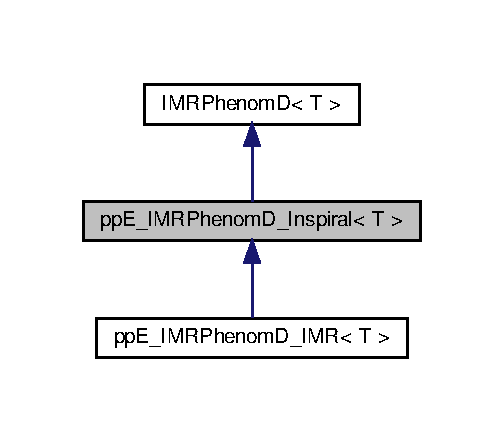
\includegraphics[width=350pt]{classppE__IMRPhenomD__Inspiral__inherit__graph}
\end{center}
\end{figure}


Collaboration diagram for pp\+E\+\_\+\+I\+M\+R\+Phenom\+D\+\_\+\+Inspiral$<$ T $>$\+:
\nopagebreak
\begin{figure}[H]
\begin{center}
\leavevmode
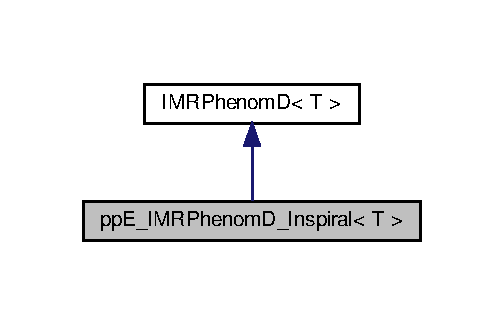
\includegraphics[width=242pt]{classppE__IMRPhenomD__Inspiral__coll__graph}
\end{center}
\end{figure}
\doxysubsection*{Public Member Functions}
\begin{DoxyCompactItemize}
\item 
\mbox{\Hypertarget{classppE__IMRPhenomD__Inspiral_a3187c9dba10e42f0bf20fb1e3bac9a52}\label{classppE__IMRPhenomD__Inspiral_a3187c9dba10e42f0bf20fb1e3bac9a52}} 
virtual T \mbox{\hyperlink{classppE__IMRPhenomD__Inspiral_a3187c9dba10e42f0bf20fb1e3bac9a52}{phase\+\_\+ins}} (T f, \mbox{\hyperlink{structsource__parameters}{source\+\_\+parameters}}$<$ T $>$ $\ast$param, T $\ast$pn\+\_\+coeff, \mbox{\hyperlink{structlambda__parameters}{lambda\+\_\+parameters}}$<$ T $>$ $\ast$lambda, \mbox{\hyperlink{structuseful__powers}{useful\+\_\+powers}}$<$ T $>$ $\ast$pow)
\begin{DoxyCompactList}\small\item\em Overloaded method for the inspiral portion of the phase. \end{DoxyCompactList}\item 
virtual T \mbox{\hyperlink{classppE__IMRPhenomD__Inspiral_ae297c077497d34a2632c55a7dafb9e83}{Dphase\+\_\+ins}} (T f, \mbox{\hyperlink{structsource__parameters}{source\+\_\+parameters}}$<$ T $>$ $\ast$param, T $\ast$pn\+\_\+coeff, \mbox{\hyperlink{structlambda__parameters}{lambda\+\_\+parameters}}$<$ T $>$ $\ast$lambda)
\begin{DoxyCompactList}\small\item\em Calculates the derivative of the inspiral phase for frequency f. \end{DoxyCompactList}\item 
\mbox{\Hypertarget{classppE__IMRPhenomD__Inspiral_ab6fe831f7c11840235dac2433ba14f82}\label{classppE__IMRPhenomD__Inspiral_ab6fe831f7c11840235dac2433ba14f82}} 
virtual void {\bfseries fisher\+\_\+calculation\+\_\+sky\+\_\+averaged} (double $\ast$frequency, int length, \mbox{\hyperlink{classgen__params}{gen\+\_\+params}} $\ast$parameters, double $\ast$$\ast$amplitude\+\_\+deriv, double $\ast$$\ast$phase\+\_\+deriv, double $\ast$amplitude, int $\ast$amp\+\_\+tapes, int $\ast$phase\+\_\+tapes)
\item 
virtual void \mbox{\hyperlink{classppE__IMRPhenomD__Inspiral_a87474cac9d6086d5625f79e28970b5ed}{amplitude\+\_\+tape}} (\mbox{\hyperlink{structsource__parameters}{source\+\_\+parameters}}$<$ double $>$ $\ast$input\+\_\+params, int $\ast$tape)
\begin{DoxyCompactList}\small\item\em Creates the tapes for derivatives of the amplitude. \end{DoxyCompactList}\item 
virtual void \mbox{\hyperlink{classppE__IMRPhenomD__Inspiral_a2fb1a8fb66e4204dbe397b792933afbe}{phase\+\_\+tape}} (\mbox{\hyperlink{structsource__parameters}{source\+\_\+parameters}}$<$ double $>$ $\ast$input\+\_\+params, int $\ast$tape)
\begin{DoxyCompactList}\small\item\em Creates the tapes for derivatives of phase. \end{DoxyCompactList}\item 
virtual void \mbox{\hyperlink{classppE__IMRPhenomD__Inspiral_a97d35197595f31d6cfbf6a8cf7c9a9ad}{construct\+\_\+amplitude\+\_\+derivative}} (double $\ast$frequencies, int length, int dimension, double $\ast$$\ast$amplitude\+\_\+derivative, \mbox{\hyperlink{structsource__parameters}{source\+\_\+parameters}}$<$ double $>$ $\ast$input\+\_\+params, int $\ast$tapes=N\+U\+LL)
\begin{DoxyCompactList}\small\item\em Construct the derivative of the amplitude for a given source evaluated by the given frequency. \end{DoxyCompactList}\item 
virtual void \mbox{\hyperlink{classppE__IMRPhenomD__Inspiral_a28d189808db2bd204e0d0051a1ed6427}{construct\+\_\+phase\+\_\+derivative}} (double $\ast$frequencies, int length, int dimension, double $\ast$$\ast$phase\+\_\+derivative, \mbox{\hyperlink{structsource__parameters}{source\+\_\+parameters}}$<$ double $>$ $\ast$input\+\_\+params, int $\ast$tapes=N\+U\+LL)
\begin{DoxyCompactList}\small\item\em Construct the derivative of the phase for a given source evaluated by the given frequency. \end{DoxyCompactList}\end{DoxyCompactItemize}


\doxysubsection{Detailed Description}
\subsubsection*{template$<$class T$>$\newline
class pp\+E\+\_\+\+I\+M\+R\+Phenom\+D\+\_\+\+Inspiral$<$ T $>$}

Class that extends the \mbox{\hyperlink{classIMRPhenomD}{I\+M\+R\+PhenomD}} waveform to include non-\/\+GR terms in the inspiral portion of the phase. This is an appropriate waveform choice for generation effects, but not necessarily for propagation effects 

\doxysubsection{Member Function Documentation}
\mbox{\Hypertarget{classppE__IMRPhenomD__Inspiral_a87474cac9d6086d5625f79e28970b5ed}\label{classppE__IMRPhenomD__Inspiral_a87474cac9d6086d5625f79e28970b5ed}} 
\index{ppE\_IMRPhenomD\_Inspiral$<$ T $>$@{ppE\_IMRPhenomD\_Inspiral$<$ T $>$}!amplitude\_tape@{amplitude\_tape}}
\index{amplitude\_tape@{amplitude\_tape}!ppE\_IMRPhenomD\_Inspiral$<$ T $>$@{ppE\_IMRPhenomD\_Inspiral$<$ T $>$}}
\doxysubsubsection{\texorpdfstring{amplitude\_tape()}{amplitude\_tape()}}
{\footnotesize\ttfamily template$<$class T $>$ \\
void \mbox{\hyperlink{classppE__IMRPhenomD__Inspiral}{pp\+E\+\_\+\+I\+M\+R\+Phenom\+D\+\_\+\+Inspiral}}$<$ T $>$\+::amplitude\+\_\+tape (\begin{DoxyParamCaption}\item[{\mbox{\hyperlink{structsource__parameters}{source\+\_\+parameters}}$<$ double $>$ $\ast$}]{input\+\_\+params,  }\item[{int $\ast$}]{tape }\end{DoxyParamCaption})\hspace{0.3cm}{\ttfamily [virtual]}}



Creates the tapes for derivatives of the amplitude. 

For efficiency in long runs of large sets of fishers, the tapes can be precomputed and reused 
\begin{DoxyParams}{Parameters}
{\em input\+\_\+params} & source parameters structure of the desired source \\
\hline
{\em tape} & tape ids \\
\hline
\end{DoxyParams}


Reimplemented from \mbox{\hyperlink{classIMRPhenomD_a6fbe3c51ee3eb66d332dc87a9fdf5bd4}{I\+M\+R\+Phenom\+D$<$ T $>$}}.



Reimplemented in \mbox{\hyperlink{classppE__IMRPhenomD__IMR_a3119a07c11ed53ae94823b11c5234c4f}{pp\+E\+\_\+\+I\+M\+R\+Phenom\+D\+\_\+\+I\+M\+R$<$ T $>$}}.

\mbox{\Hypertarget{classppE__IMRPhenomD__Inspiral_a97d35197595f31d6cfbf6a8cf7c9a9ad}\label{classppE__IMRPhenomD__Inspiral_a97d35197595f31d6cfbf6a8cf7c9a9ad}} 
\index{ppE\_IMRPhenomD\_Inspiral$<$ T $>$@{ppE\_IMRPhenomD\_Inspiral$<$ T $>$}!construct\_amplitude\_derivative@{construct\_amplitude\_derivative}}
\index{construct\_amplitude\_derivative@{construct\_amplitude\_derivative}!ppE\_IMRPhenomD\_Inspiral$<$ T $>$@{ppE\_IMRPhenomD\_Inspiral$<$ T $>$}}
\doxysubsubsection{\texorpdfstring{construct\_amplitude\_derivative()}{construct\_amplitude\_derivative()}}
{\footnotesize\ttfamily template$<$class T $>$ \\
void \mbox{\hyperlink{classppE__IMRPhenomD__Inspiral}{pp\+E\+\_\+\+I\+M\+R\+Phenom\+D\+\_\+\+Inspiral}}$<$ T $>$\+::construct\+\_\+amplitude\+\_\+derivative (\begin{DoxyParamCaption}\item[{double $\ast$}]{frequencies,  }\item[{int}]{length,  }\item[{int}]{dimension,  }\item[{double $\ast$$\ast$}]{amplitude\+\_\+derivative,  }\item[{\mbox{\hyperlink{structsource__parameters}{source\+\_\+parameters}}$<$ double $>$ $\ast$}]{input\+\_\+params,  }\item[{int $\ast$}]{tapes = {\ttfamily NULL} }\end{DoxyParamCaption})\hspace{0.3cm}{\ttfamily [virtual]}}



Construct the derivative of the amplitude for a given source evaluated by the given frequency. 

Order of output\+: dh/d \textbackslash{}theta \+: \textbackslash{}theta \textbackslash{}el \{A0,tc, phic, chirp mass, eta, symmetric spin, antisymmetric spin\} 
\begin{DoxyParams}{Parameters}
{\em frequencies} & input array of frequency \\
\hline
{\em length} & length of the frequency array \\
\hline
{\em amplitude\+\_\+derivative} & $<$ dimension of the fisher output array for all the derivatives double\mbox{[}dimension\mbox{]}\mbox{[}length\mbox{]} \\
\hline
{\em input\+\_\+params} & Source parameters structure for the source \\
\hline
{\em tapes} & int array of tape ids, if N\+U\+LL, these will be calculated \\
\hline
\end{DoxyParams}


Reimplemented from \mbox{\hyperlink{classIMRPhenomD_a4142331cc7a6471d13274b1ac8727378}{I\+M\+R\+Phenom\+D$<$ T $>$}}.



Reimplemented in \mbox{\hyperlink{classppE__IMRPhenomD__IMR_a5b80e5ae4dd83da49beb15e6e5f17715}{pp\+E\+\_\+\+I\+M\+R\+Phenom\+D\+\_\+\+I\+M\+R$<$ T $>$}}.

\mbox{\Hypertarget{classppE__IMRPhenomD__Inspiral_a28d189808db2bd204e0d0051a1ed6427}\label{classppE__IMRPhenomD__Inspiral_a28d189808db2bd204e0d0051a1ed6427}} 
\index{ppE\_IMRPhenomD\_Inspiral$<$ T $>$@{ppE\_IMRPhenomD\_Inspiral$<$ T $>$}!construct\_phase\_derivative@{construct\_phase\_derivative}}
\index{construct\_phase\_derivative@{construct\_phase\_derivative}!ppE\_IMRPhenomD\_Inspiral$<$ T $>$@{ppE\_IMRPhenomD\_Inspiral$<$ T $>$}}
\doxysubsubsection{\texorpdfstring{construct\_phase\_derivative()}{construct\_phase\_derivative()}}
{\footnotesize\ttfamily template$<$class T $>$ \\
void \mbox{\hyperlink{classppE__IMRPhenomD__Inspiral}{pp\+E\+\_\+\+I\+M\+R\+Phenom\+D\+\_\+\+Inspiral}}$<$ T $>$\+::construct\+\_\+phase\+\_\+derivative (\begin{DoxyParamCaption}\item[{double $\ast$}]{frequencies,  }\item[{int}]{length,  }\item[{int}]{dimension,  }\item[{double $\ast$$\ast$}]{phase\+\_\+derivative,  }\item[{\mbox{\hyperlink{structsource__parameters}{source\+\_\+parameters}}$<$ double $>$ $\ast$}]{input\+\_\+params,  }\item[{int $\ast$}]{tapes = {\ttfamily NULL} }\end{DoxyParamCaption})\hspace{0.3cm}{\ttfamily [virtual]}}



Construct the derivative of the phase for a given source evaluated by the given frequency. 

Order of output\+: dh/d \textbackslash{}theta \+: \textbackslash{}theta \textbackslash{}el \{A0,tc, phic, chirp mass, eta, symmetric spin, antisymmetric spin\} 
\begin{DoxyParams}{Parameters}
{\em frequencies} & input array of frequency \\
\hline
{\em length} & length of the frequency array \\
\hline
{\em phase\+\_\+derivative} & $<$ dimension of the fisher output array for all the derivatives double\mbox{[}dimension\mbox{]}\mbox{[}length\mbox{]} \\
\hline
{\em input\+\_\+params} & Source parameters structure for the source \\
\hline
{\em tapes} & int array of tape ids, if N\+U\+LL, these will be calculated \\
\hline
\end{DoxyParams}


Reimplemented from \mbox{\hyperlink{classIMRPhenomD_a26da276caf4c148016f558541d6914f6}{I\+M\+R\+Phenom\+D$<$ T $>$}}.



Reimplemented in \mbox{\hyperlink{classppE__IMRPhenomD__IMR_a78151d1f34693b69cf6ccbc28df4caa6}{pp\+E\+\_\+\+I\+M\+R\+Phenom\+D\+\_\+\+I\+M\+R$<$ T $>$}}.

\mbox{\Hypertarget{classppE__IMRPhenomD__Inspiral_ae297c077497d34a2632c55a7dafb9e83}\label{classppE__IMRPhenomD__Inspiral_ae297c077497d34a2632c55a7dafb9e83}} 
\index{ppE\_IMRPhenomD\_Inspiral$<$ T $>$@{ppE\_IMRPhenomD\_Inspiral$<$ T $>$}!Dphase\_ins@{Dphase\_ins}}
\index{Dphase\_ins@{Dphase\_ins}!ppE\_IMRPhenomD\_Inspiral$<$ T $>$@{ppE\_IMRPhenomD\_Inspiral$<$ T $>$}}
\doxysubsubsection{\texorpdfstring{Dphase\_ins()}{Dphase\_ins()}}
{\footnotesize\ttfamily template$<$class T $>$ \\
T \mbox{\hyperlink{classppE__IMRPhenomD__Inspiral}{pp\+E\+\_\+\+I\+M\+R\+Phenom\+D\+\_\+\+Inspiral}}$<$ T $>$\+::Dphase\+\_\+ins (\begin{DoxyParamCaption}\item[{T}]{f,  }\item[{\mbox{\hyperlink{structsource__parameters}{source\+\_\+parameters}}$<$ T $>$ $\ast$}]{param,  }\item[{T $\ast$}]{pn\+\_\+coeff,  }\item[{\mbox{\hyperlink{structlambda__parameters}{lambda\+\_\+parameters}}$<$ T $>$ $\ast$}]{lambda }\end{DoxyParamCaption})\hspace{0.3cm}{\ttfamily [virtual]}}



Calculates the derivative of the inspiral phase for frequency f. 

For phase continuity and smoothness return a T 

Reimplemented from \mbox{\hyperlink{classIMRPhenomD_ab840b052576cde8a9e802c5784d24092}{I\+M\+R\+Phenom\+D$<$ T $>$}}.

\mbox{\Hypertarget{classppE__IMRPhenomD__Inspiral_a2fb1a8fb66e4204dbe397b792933afbe}\label{classppE__IMRPhenomD__Inspiral_a2fb1a8fb66e4204dbe397b792933afbe}} 
\index{ppE\_IMRPhenomD\_Inspiral$<$ T $>$@{ppE\_IMRPhenomD\_Inspiral$<$ T $>$}!phase\_tape@{phase\_tape}}
\index{phase\_tape@{phase\_tape}!ppE\_IMRPhenomD\_Inspiral$<$ T $>$@{ppE\_IMRPhenomD\_Inspiral$<$ T $>$}}
\doxysubsubsection{\texorpdfstring{phase\_tape()}{phase\_tape()}}
{\footnotesize\ttfamily template$<$class T $>$ \\
void \mbox{\hyperlink{classppE__IMRPhenomD__Inspiral}{pp\+E\+\_\+\+I\+M\+R\+Phenom\+D\+\_\+\+Inspiral}}$<$ T $>$\+::phase\+\_\+tape (\begin{DoxyParamCaption}\item[{\mbox{\hyperlink{structsource__parameters}{source\+\_\+parameters}}$<$ double $>$ $\ast$}]{input\+\_\+params,  }\item[{int $\ast$}]{tape }\end{DoxyParamCaption})\hspace{0.3cm}{\ttfamily [virtual]}}



Creates the tapes for derivatives of phase. 

For efficiency in long runs of large sets of fishers, the tapes can be precomputed and reused 
\begin{DoxyParams}{Parameters}
{\em input\+\_\+params} & source parameters structure of the desired source \\
\hline
{\em tape} & tape ids \\
\hline
\end{DoxyParams}


Reimplemented from \mbox{\hyperlink{classIMRPhenomD_ae456c25f87c34487e6e05f9cf5d2d08c}{I\+M\+R\+Phenom\+D$<$ T $>$}}.



Reimplemented in \mbox{\hyperlink{classppE__IMRPhenomD__IMR_acf2ed8617b3e24ecc273a409ff579ce4}{pp\+E\+\_\+\+I\+M\+R\+Phenom\+D\+\_\+\+I\+M\+R$<$ T $>$}}.



The documentation for this class was generated from the following files\+:\begin{DoxyCompactItemize}
\item 
include/gwat/\mbox{\hyperlink{ppE__IMRPhenomD_8h}{pp\+E\+\_\+\+I\+M\+R\+Phenom\+D.\+h}}\item 
src/\mbox{\hyperlink{ppE__IMRPhenomD_8cpp}{pp\+E\+\_\+\+I\+M\+R\+Phenom\+D.\+cpp}}\end{DoxyCompactItemize}

\hypertarget{structsource__parameters}{}\doxysection{source\+\_\+parameters$<$ T $>$ Struct Template Reference}
\label{structsource__parameters}\index{source\_parameters$<$ T $>$@{source\_parameters$<$ T $>$}}
\doxysubsection*{Static Public Member Functions}
\begin{DoxyCompactItemize}
\item 
static \mbox{\hyperlink{structsource__parameters}{source\+\_\+parameters}}$<$ T $>$ \mbox{\hyperlink{structsource__parameters_aa6b0e1aa5122c2887a3db4d40714ac84}{populate\+\_\+source\+\_\+parameters}} (\mbox{\hyperlink{classgen__params__base}{gen\+\_\+params\+\_\+base}}$<$ T $>$ $\ast$param\+\_\+in)
\begin{DoxyCompactList}\small\item\em Builds the structure that shuttles source parameters between functions -\/updated version to incorporate structure argument. \end{DoxyCompactList}\item 
static \mbox{\hyperlink{structsource__parameters}{source\+\_\+parameters}}$<$ T $>$ \mbox{\hyperlink{structsource__parameters_a1b9db2c7d8abf202ca908fd4e58b0949}{populate\+\_\+source\+\_\+parameters\+\_\+old}} (T \mbox{\hyperlink{structsource__parameters_a1a222ddfbc43359da566d085d92e7b72}{mass1}}, T \mbox{\hyperlink{structsource__parameters_a889d5e8ae96cec656504784f19916b5d}{mass2}}, T Luminosity\+\_\+\+Distance, T $\ast$spin1, T $\ast$spin2, T phi\+\_\+c, T t\+\_\+c, bool sky\+\_\+average)
\begin{DoxyCompactList}\small\item\em Builds the structure that shuttles source parameters between functions-\/ outdated in favor of structure argument. \end{DoxyCompactList}\end{DoxyCompactItemize}
\doxysubsection*{Public Attributes}
\begin{DoxyCompactItemize}
\item 
T \mbox{\hyperlink{structsource__parameters_a1a222ddfbc43359da566d085d92e7b72}{mass1}}
\item 
T \mbox{\hyperlink{structsource__parameters_a889d5e8ae96cec656504784f19916b5d}{mass2}}
\item 
T \mbox{\hyperlink{structsource__parameters_a52eefefefdf8c0bc989b64a115aed48a}{M}}
\item 
\mbox{\Hypertarget{structsource__parameters_a5124b374fbac884c79c7d97e2dfad392}\label{structsource__parameters_a5124b374fbac884c79c7d97e2dfad392}} 
T {\bfseries q}
\item 
T \mbox{\hyperlink{structsource__parameters_a4184da329b8db0612133d4202f5f2769}{spin1z}}
\item 
T \mbox{\hyperlink{structsource__parameters_a1dfb782bc530dd8bc64a8a454da4e698}{spin2z}}
\item 
T \mbox{\hyperlink{structsource__parameters_a7112cbffca6f374199399cb2a4676440}{spin1x}}
\item 
T \mbox{\hyperlink{structsource__parameters_ac5278ad7984fb12f6a0c0277d6c6f25e}{spin2x}}
\item 
T \mbox{\hyperlink{structsource__parameters_aee9a22b3a44293741d68b303f0b40c06}{spin1y}}
\item 
T \mbox{\hyperlink{structsource__parameters_a7f457ff3d231ba2f254570a7e09f45f9}{spin2y}}
\item 
T \mbox{\hyperlink{structsource__parameters_a45ed5fee56015020945397cad4090c0b}{chirpmass}}
\item 
T \mbox{\hyperlink{structsource__parameters_ad0c3de98a95860855de219af0e095e81}{eta}}
\item 
T \mbox{\hyperlink{structsource__parameters_a795a4c996933c8096dc507fb4b77660c}{chi\+\_\+s}}
\item 
T \mbox{\hyperlink{structsource__parameters_abb7188532f4129d5b952aa040ca2a68f}{chi\+\_\+a}}
\item 
T \mbox{\hyperlink{structsource__parameters_af76e6fbb66cdb45dc7ce96eb7ff1440c}{chi\+\_\+eff}}
\item 
T \mbox{\hyperlink{structsource__parameters_aa1898ec9379fb825dd3a327292e7466e}{chi\+\_\+pn}}
\item 
T \mbox{\hyperlink{structsource__parameters_a3b63b38f49f875e1d9cc150c5753aa3c}{DL}}
\item 
T \mbox{\hyperlink{structsource__parameters_a6485c9fc5622ab2cd81170ceef81db66}{delta\+\_\+mass}}
\item 
T \mbox{\hyperlink{structsource__parameters_ad221b8f66ef2d9fd878b1c70461b60db}{f\+RD}}
\item 
T \mbox{\hyperlink{structsource__parameters_adf9f63901b2a77eb0b89bba6ff68239e}{fdamp}}
\item 
T \mbox{\hyperlink{structsource__parameters_af053aa1c29b1fae75333ca7ac166e81c}{f1}}
\item 
T \mbox{\hyperlink{structsource__parameters_aea5ffd30832405cf32b6fa4d9fbd3ae6}{f3}}
\item 
T \mbox{\hyperlink{structsource__parameters_a41904030076ceee4599d6f22ff011daa}{f1\+\_\+phase}}
\item 
T \mbox{\hyperlink{structsource__parameters_a5ce4351ddc8a19f02c5475a7bcaa8e8d}{f2\+\_\+phase}}
\item 
T \mbox{\hyperlink{structsource__parameters_a60cbeb524afa4f18cc5c47b0b43c3c18}{phic}}
\item 
T \mbox{\hyperlink{structsource__parameters_ac0c03ead9615b4c9f27d160ad023db70}{tc}}
\item 
\mbox{\Hypertarget{structsource__parameters_a8153a3eb546d1da6d7de74a5b713edd8}\label{structsource__parameters_a8153a3eb546d1da6d7de74a5b713edd8}} 
T {\bfseries A0}
\item 
bool \mbox{\hyperlink{structsource__parameters_aa49fc4d87dfa45e9837ee70d97694882}{shift\+\_\+phase}} = true
\item 
\mbox{\Hypertarget{structsource__parameters_a59da58a808b3f00d8f19acfc3b4aa29f}\label{structsource__parameters_a59da58a808b3f00d8f19acfc3b4aa29f}} 
bool {\bfseries N\+Sflag1}
\item 
\mbox{\Hypertarget{structsource__parameters_a962651040c37f61c5e6d1f5c45a1f41d}\label{structsource__parameters_a962651040c37f61c5e6d1f5c45a1f41d}} 
bool {\bfseries N\+Sflag2}
\item 
\mbox{\Hypertarget{structsource__parameters_a7c6e23c98318c7ab1a4aa59e18cbdbf0}\label{structsource__parameters_a7c6e23c98318c7ab1a4aa59e18cbdbf0}} 
T {\bfseries s}
\item 
\mbox{\Hypertarget{structsource__parameters_aa3ee855a28f38ac92abe1458f4334221}\label{structsource__parameters_aa3ee855a28f38ac92abe1458f4334221}} 
T {\bfseries chil}
\item 
\mbox{\Hypertarget{structsource__parameters_a8c3c8bb7dcb7258e4ddd2dce5f2b633a}\label{structsource__parameters_a8c3c8bb7dcb7258e4ddd2dce5f2b633a}} 
T {\bfseries chip}
\item 
\mbox{\Hypertarget{structsource__parameters_aaab7aa48e3f89cadaa2b1c768f1ab0d1}\label{structsource__parameters_aaab7aa48e3f89cadaa2b1c768f1ab0d1}} 
T {\bfseries phip} = -\/1
\item 
\mbox{\Hypertarget{structsource__parameters_ab8f0e9795b3a39a788c7ff07ea15f370}\label{structsource__parameters_ab8f0e9795b3a39a788c7ff07ea15f370}} 
T {\bfseries f\+\_\+ref} =0
\item 
\mbox{\Hypertarget{structsource__parameters_a0b50846d1e17e9cded5879e3ecc76841}\label{structsource__parameters_a0b50846d1e17e9cded5879e3ecc76841}} 
T {\bfseries phi\+\_\+aligned}
\item 
\mbox{\Hypertarget{structsource__parameters_ac5e4063546d79ec62ff793ec5363b20d}\label{structsource__parameters_ac5e4063546d79ec62ff793ec5363b20d}} 
T {\bfseries incl\+\_\+angle}
\item 
\mbox{\Hypertarget{structsource__parameters_a9f287773c706c559ea190229ff0773b4}\label{structsource__parameters_a9f287773c706c559ea190229ff0773b4}} 
T {\bfseries phi\+Ref}
\item 
\mbox{\Hypertarget{structsource__parameters_aab3eb0a82eb97db0a49aaff255af0d60}\label{structsource__parameters_aab3eb0a82eb97db0a49aaff255af0d60}} 
T {\bfseries alpha0}
\item 
\mbox{\Hypertarget{structsource__parameters_a9ce5feb101d4e4337df905a288f71e0e}\label{structsource__parameters_a9ce5feb101d4e4337df905a288f71e0e}} 
T {\bfseries theta\+JN}
\item 
\mbox{\Hypertarget{structsource__parameters_a7a4c0c4c3847c4e632b5bef3bb32155c}\label{structsource__parameters_a7a4c0c4c3847c4e632b5bef3bb32155c}} 
T {\bfseries zeta\+\_\+polariz}
\item 
\mbox{\Hypertarget{structsource__parameters_a0638be3609f73afa73d95c4db571e8a9}\label{structsource__parameters_a0638be3609f73afa73d95c4db571e8a9}} 
T {\bfseries chi1\+\_\+p} = 0
\item 
\mbox{\Hypertarget{structsource__parameters_a88919e3d60ff1703f3d68073456eeb9d}\label{structsource__parameters_a88919e3d60ff1703f3d68073456eeb9d}} 
T {\bfseries chi2\+\_\+p} = 0
\item 
\mbox{\Hypertarget{structsource__parameters_a4bdb088e6eca1c0a64d055ba75f1eecd}\label{structsource__parameters_a4bdb088e6eca1c0a64d055ba75f1eecd}} 
T {\bfseries chi1\+\_\+l} = 0
\item 
\mbox{\Hypertarget{structsource__parameters_ab5c01e8580cf46bf08d52e7763886b0f}\label{structsource__parameters_ab5c01e8580cf46bf08d52e7763886b0f}} 
T {\bfseries chi2\+\_\+l} = 0
\item 
\mbox{\Hypertarget{structsource__parameters_a6d6642a6ac2b70e0ed5c7a56e3b3372c}\label{structsource__parameters_a6d6642a6ac2b70e0ed5c7a56e3b3372c}} 
T {\bfseries phi\+JL} = 0
\item 
\mbox{\Hypertarget{structsource__parameters_acaead03dd2e7f25d9ccedd1cafc9f336}\label{structsource__parameters_acaead03dd2e7f25d9ccedd1cafc9f336}} 
T {\bfseries theta\+JL} = -\/1
\item 
\mbox{\Hypertarget{structsource__parameters_adce0e179be1c7a14db7c4c852fd6be03}\label{structsource__parameters_adce0e179be1c7a14db7c4c852fd6be03}} 
T $\ast$ {\bfseries betappe}
\item 
\mbox{\Hypertarget{structsource__parameters_a6c7169f21a35abbac204c83606c711a4}\label{structsource__parameters_a6c7169f21a35abbac204c83606c711a4}} 
int $\ast$ {\bfseries bppe}
\item 
int \mbox{\hyperlink{structsource__parameters_a0c0678c3881ae1e62819c685b119d065}{Nmod}}
\item 
\mbox{\Hypertarget{structsource__parameters_ac9b7d9ce563fe8e9241e5b9165746b13}\label{structsource__parameters_ac9b7d9ce563fe8e9241e5b9165746b13}} 
T {\bfseries phi}
\item 
\mbox{\Hypertarget{structsource__parameters_ad396ba7ec20fd6b3a9469b8a78fa2ea4}\label{structsource__parameters_ad396ba7ec20fd6b3a9469b8a78fa2ea4}} 
T {\bfseries theta}
\item 
\mbox{\Hypertarget{structsource__parameters_a3a575130238c416b568689ebfa1c18d5}\label{structsource__parameters_a3a575130238c416b568689ebfa1c18d5}} 
T {\bfseries SP}
\item 
\mbox{\Hypertarget{structsource__parameters_a2199aebd16bde1243d2ca16f02f4a533}\label{structsource__parameters_a2199aebd16bde1243d2ca16f02f4a533}} 
T {\bfseries SL}
\item 
\mbox{\Hypertarget{structsource__parameters_a74e2df5e9bd0e68f5c712a1a0f14f3ef}\label{structsource__parameters_a74e2df5e9bd0e68f5c712a1a0f14f3ef}} 
bool {\bfseries sky\+\_\+average}
\item 
bool \mbox{\hyperlink{structsource__parameters_acc29cebe856d34141837e5c118c31d70}{shift\+\_\+time}} = true
\item 
\mbox{\Hypertarget{structsource__parameters_a490daa8916bb550275f05da618d984b6}\label{structsource__parameters_a490daa8916bb550275f05da618d984b6}} 
gsl\+\_\+spline $\ast$ {\bfseries Z\+\_\+\+D\+L\+\_\+spline\+\_\+ptr} =N\+U\+LL
\item 
\mbox{\Hypertarget{structsource__parameters_ae079ce586d3f1cdeb97c4dc82ca4629c}\label{structsource__parameters_ae079ce586d3f1cdeb97c4dc82ca4629c}} 
gsl\+\_\+interp\+\_\+accel $\ast$ {\bfseries Z\+\_\+\+D\+L\+\_\+accel\+\_\+ptr} =N\+U\+LL
\item 
\mbox{\Hypertarget{structsource__parameters_a4d3dc9f50b809a05b1110d8f9e115945}\label{structsource__parameters_a4d3dc9f50b809a05b1110d8f9e115945}} 
std\+::string {\bfseries cosmology}
\item 
\mbox{\Hypertarget{structsource__parameters_ac5bd295489af2cf3ce84c74521c75a3c}\label{structsource__parameters_ac5bd295489af2cf3ce84c74521c75a3c}} 
int {\bfseries Nmod\+\_\+beta} =0
\item 
\mbox{\Hypertarget{structsource__parameters_ab679f2cef3b07cf30c031e22550f0af5}\label{structsource__parameters_ab679f2cef3b07cf30c031e22550f0af5}} 
int {\bfseries Nmod\+\_\+alpha} =0
\item 
\mbox{\Hypertarget{structsource__parameters_ac5a6acbe627a89efba623d4b4272da45}\label{structsource__parameters_ac5a6acbe627a89efba623d4b4272da45}} 
int {\bfseries Nmod\+\_\+sigma} =0
\item 
\mbox{\Hypertarget{structsource__parameters_a4746d6a950182fede9ee405927219dab}\label{structsource__parameters_a4746d6a950182fede9ee405927219dab}} 
int {\bfseries Nmod\+\_\+phi} =0
\item 
\mbox{\Hypertarget{structsource__parameters_a2805aea47ebccdd6528cc6213191744b}\label{structsource__parameters_a2805aea47ebccdd6528cc6213191744b}} 
int $\ast$ {\bfseries betai}
\item 
\mbox{\Hypertarget{structsource__parameters_a02e8a88049ca3f46462ad2e97a839c9c}\label{structsource__parameters_a02e8a88049ca3f46462ad2e97a839c9c}} 
int $\ast$ {\bfseries alphai}
\item 
\mbox{\Hypertarget{structsource__parameters_ae933bd3784481c21d0614601af68da36}\label{structsource__parameters_ae933bd3784481c21d0614601af68da36}} 
int $\ast$ {\bfseries sigmai}
\item 
\mbox{\Hypertarget{structsource__parameters_a753157760fe4a88dc5550bb3eaad8eba}\label{structsource__parameters_a753157760fe4a88dc5550bb3eaad8eba}} 
int $\ast$ {\bfseries phii}
\item 
\mbox{\Hypertarget{structsource__parameters_aa423ed663aac3bc997e257641f848144}\label{structsource__parameters_aa423ed663aac3bc997e257641f848144}} 
T $\ast$ {\bfseries delta\+\_\+beta}
\item 
\mbox{\Hypertarget{structsource__parameters_a0acf708593c3e0f343736ff7a9bcd0c0}\label{structsource__parameters_a0acf708593c3e0f343736ff7a9bcd0c0}} 
T $\ast$ {\bfseries delta\+\_\+alpha}
\item 
\mbox{\Hypertarget{structsource__parameters_a5252a829be6b042a69259dc94e33d67f}\label{structsource__parameters_a5252a829be6b042a69259dc94e33d67f}} 
T $\ast$ {\bfseries delta\+\_\+sigma}
\item 
\mbox{\Hypertarget{structsource__parameters_aaf22d477f9f74174de6ee4b3ae691b9b}\label{structsource__parameters_aaf22d477f9f74174de6ee4b3ae691b9b}} 
T $\ast$ {\bfseries delta\+\_\+phi}
\end{DoxyCompactItemize}


\doxysubsection{Member Function Documentation}
\mbox{\Hypertarget{structsource__parameters_aa6b0e1aa5122c2887a3db4d40714ac84}\label{structsource__parameters_aa6b0e1aa5122c2887a3db4d40714ac84}} 
\index{source\_parameters$<$ T $>$@{source\_parameters$<$ T $>$}!populate\_source\_parameters@{populate\_source\_parameters}}
\index{populate\_source\_parameters@{populate\_source\_parameters}!source\_parameters$<$ T $>$@{source\_parameters$<$ T $>$}}
\doxysubsubsection{\texorpdfstring{populate\_source\_parameters()}{populate\_source\_parameters()}}
{\footnotesize\ttfamily template$<$class T $>$ \\
\mbox{\hyperlink{structsource__parameters}{source\+\_\+parameters}}$<$ T $>$ \mbox{\hyperlink{structsource__parameters}{source\+\_\+parameters}}$<$ T $>$\+::populate\+\_\+source\+\_\+parameters (\begin{DoxyParamCaption}\item[{\mbox{\hyperlink{classgen__params__base}{gen\+\_\+params\+\_\+base}}$<$ T $>$ $\ast$}]{param\+\_\+in }\end{DoxyParamCaption})\hspace{0.3cm}{\ttfamily [static]}}



Builds the structure that shuttles source parameters between functions -\/updated version to incorporate structure argument. 

Populates the structure that is passed to all generation methods -\/ contains all relavent source parameters

Template type of source parameters and gen\+\_\+parameters must match \mbox{\Hypertarget{structsource__parameters_a1b9db2c7d8abf202ca908fd4e58b0949}\label{structsource__parameters_a1b9db2c7d8abf202ca908fd4e58b0949}} 
\index{source\_parameters$<$ T $>$@{source\_parameters$<$ T $>$}!populate\_source\_parameters\_old@{populate\_source\_parameters\_old}}
\index{populate\_source\_parameters\_old@{populate\_source\_parameters\_old}!source\_parameters$<$ T $>$@{source\_parameters$<$ T $>$}}
\doxysubsubsection{\texorpdfstring{populate\_source\_parameters\_old()}{populate\_source\_parameters\_old()}}
{\footnotesize\ttfamily template$<$class T $>$ \\
\mbox{\hyperlink{structsource__parameters}{source\+\_\+parameters}}$<$ T $>$ \mbox{\hyperlink{structsource__parameters}{source\+\_\+parameters}}$<$ T $>$\+::populate\+\_\+source\+\_\+parameters\+\_\+old (\begin{DoxyParamCaption}\item[{T}]{mass1,  }\item[{T}]{mass2,  }\item[{T}]{Luminosity\+\_\+\+Distance,  }\item[{T $\ast$}]{spin1,  }\item[{T $\ast$}]{spin2,  }\item[{T}]{phi\+\_\+c,  }\item[{T}]{t\+\_\+c,  }\item[{bool}]{sky\+\_\+average }\end{DoxyParamCaption})\hspace{0.3cm}{\ttfamily [static]}}



Builds the structure that shuttles source parameters between functions-\/ outdated in favor of structure argument. 

Populates the structure that is passed to all generation methods -\/ contains all relavent source parameters 
\begin{DoxyParams}{Parameters}
{\em mass1} & mass of the larger body -\/ in Solar Masses \\
\hline
{\em mass2} & mass of the smaller body -\/ in Solar Masses \\
\hline
{\em Luminosity\+\_\+\+Distance} & Luminosity Distance in Mpc \\
\hline
{\em spin2} & spin vector of the larger body \{sx,sy,sz\} \\
\hline
{\em phi\+\_\+c} & spin vector of the smaller body \{sx,sy,sz\} \\
\hline
{\em t\+\_\+c} & coalescence phase \\
\hline
{\em sky\+\_\+average} & coalescence time \\
\hline
\end{DoxyParams}


\doxysubsection{Member Data Documentation}
\mbox{\Hypertarget{structsource__parameters_abb7188532f4129d5b952aa040ca2a68f}\label{structsource__parameters_abb7188532f4129d5b952aa040ca2a68f}} 
\index{source\_parameters$<$ T $>$@{source\_parameters$<$ T $>$}!chi\_a@{chi\_a}}
\index{chi\_a@{chi\_a}!source\_parameters$<$ T $>$@{source\_parameters$<$ T $>$}}
\doxysubsubsection{\texorpdfstring{chi\_a}{chi\_a}}
{\footnotesize\ttfamily template$<$class T$>$ \\
T \mbox{\hyperlink{structsource__parameters}{source\+\_\+parameters}}$<$ T $>$\+::chi\+\_\+a}

Antisymmetric spin combination \mbox{\Hypertarget{structsource__parameters_af76e6fbb66cdb45dc7ce96eb7ff1440c}\label{structsource__parameters_af76e6fbb66cdb45dc7ce96eb7ff1440c}} 
\index{source\_parameters$<$ T $>$@{source\_parameters$<$ T $>$}!chi\_eff@{chi\_eff}}
\index{chi\_eff@{chi\_eff}!source\_parameters$<$ T $>$@{source\_parameters$<$ T $>$}}
\doxysubsubsection{\texorpdfstring{chi\_eff}{chi\_eff}}
{\footnotesize\ttfamily template$<$class T$>$ \\
T \mbox{\hyperlink{structsource__parameters}{source\+\_\+parameters}}$<$ T $>$\+::chi\+\_\+eff}

Effective spin \mbox{\Hypertarget{structsource__parameters_aa1898ec9379fb825dd3a327292e7466e}\label{structsource__parameters_aa1898ec9379fb825dd3a327292e7466e}} 
\index{source\_parameters$<$ T $>$@{source\_parameters$<$ T $>$}!chi\_pn@{chi\_pn}}
\index{chi\_pn@{chi\_pn}!source\_parameters$<$ T $>$@{source\_parameters$<$ T $>$}}
\doxysubsubsection{\texorpdfstring{chi\_pn}{chi\_pn}}
{\footnotesize\ttfamily template$<$class T$>$ \\
T \mbox{\hyperlink{structsource__parameters}{source\+\_\+parameters}}$<$ T $>$\+::chi\+\_\+pn}

PN spin \mbox{\Hypertarget{structsource__parameters_a795a4c996933c8096dc507fb4b77660c}\label{structsource__parameters_a795a4c996933c8096dc507fb4b77660c}} 
\index{source\_parameters$<$ T $>$@{source\_parameters$<$ T $>$}!chi\_s@{chi\_s}}
\index{chi\_s@{chi\_s}!source\_parameters$<$ T $>$@{source\_parameters$<$ T $>$}}
\doxysubsubsection{\texorpdfstring{chi\_s}{chi\_s}}
{\footnotesize\ttfamily template$<$class T$>$ \\
T \mbox{\hyperlink{structsource__parameters}{source\+\_\+parameters}}$<$ T $>$\+::chi\+\_\+s}

Symmetric spin combination \mbox{\Hypertarget{structsource__parameters_a45ed5fee56015020945397cad4090c0b}\label{structsource__parameters_a45ed5fee56015020945397cad4090c0b}} 
\index{source\_parameters$<$ T $>$@{source\_parameters$<$ T $>$}!chirpmass@{chirpmass}}
\index{chirpmass@{chirpmass}!source\_parameters$<$ T $>$@{source\_parameters$<$ T $>$}}
\doxysubsubsection{\texorpdfstring{chirpmass}{chirpmass}}
{\footnotesize\ttfamily template$<$class T$>$ \\
T \mbox{\hyperlink{structsource__parameters}{source\+\_\+parameters}}$<$ T $>$\+::chirpmass}

Chirp mass of the binary \mbox{\Hypertarget{structsource__parameters_a6485c9fc5622ab2cd81170ceef81db66}\label{structsource__parameters_a6485c9fc5622ab2cd81170ceef81db66}} 
\index{source\_parameters$<$ T $>$@{source\_parameters$<$ T $>$}!delta\_mass@{delta\_mass}}
\index{delta\_mass@{delta\_mass}!source\_parameters$<$ T $>$@{source\_parameters$<$ T $>$}}
\doxysubsubsection{\texorpdfstring{delta\_mass}{delta\_mass}}
{\footnotesize\ttfamily template$<$class T$>$ \\
T \mbox{\hyperlink{structsource__parameters}{source\+\_\+parameters}}$<$ T $>$\+::delta\+\_\+mass}

Delta mass comibination \mbox{\Hypertarget{structsource__parameters_a3b63b38f49f875e1d9cc150c5753aa3c}\label{structsource__parameters_a3b63b38f49f875e1d9cc150c5753aa3c}} 
\index{source\_parameters$<$ T $>$@{source\_parameters$<$ T $>$}!DL@{DL}}
\index{DL@{DL}!source\_parameters$<$ T $>$@{source\_parameters$<$ T $>$}}
\doxysubsubsection{\texorpdfstring{DL}{DL}}
{\footnotesize\ttfamily template$<$class T$>$ \\
T \mbox{\hyperlink{structsource__parameters}{source\+\_\+parameters}}$<$ T $>$\+::DL}

Luminoisity Distance \mbox{\Hypertarget{structsource__parameters_ad0c3de98a95860855de219af0e095e81}\label{structsource__parameters_ad0c3de98a95860855de219af0e095e81}} 
\index{source\_parameters$<$ T $>$@{source\_parameters$<$ T $>$}!eta@{eta}}
\index{eta@{eta}!source\_parameters$<$ T $>$@{source\_parameters$<$ T $>$}}
\doxysubsubsection{\texorpdfstring{eta}{eta}}
{\footnotesize\ttfamily template$<$class T$>$ \\
T \mbox{\hyperlink{structsource__parameters}{source\+\_\+parameters}}$<$ T $>$\+::eta}

Symmetric mass ratio \mbox{\Hypertarget{structsource__parameters_af053aa1c29b1fae75333ca7ac166e81c}\label{structsource__parameters_af053aa1c29b1fae75333ca7ac166e81c}} 
\index{source\_parameters$<$ T $>$@{source\_parameters$<$ T $>$}!f1@{f1}}
\index{f1@{f1}!source\_parameters$<$ T $>$@{source\_parameters$<$ T $>$}}
\doxysubsubsection{\texorpdfstring{f1}{f1}}
{\footnotesize\ttfamily template$<$class T$>$ \\
T \mbox{\hyperlink{structsource__parameters}{source\+\_\+parameters}}$<$ T $>$\+::f1}

Transition Frequency 1 for the amplitude \mbox{\Hypertarget{structsource__parameters_a41904030076ceee4599d6f22ff011daa}\label{structsource__parameters_a41904030076ceee4599d6f22ff011daa}} 
\index{source\_parameters$<$ T $>$@{source\_parameters$<$ T $>$}!f1\_phase@{f1\_phase}}
\index{f1\_phase@{f1\_phase}!source\_parameters$<$ T $>$@{source\_parameters$<$ T $>$}}
\doxysubsubsection{\texorpdfstring{f1\_phase}{f1\_phase}}
{\footnotesize\ttfamily template$<$class T$>$ \\
T \mbox{\hyperlink{structsource__parameters}{source\+\_\+parameters}}$<$ T $>$\+::f1\+\_\+phase}

Transition frequency 1 for the phase \mbox{\Hypertarget{structsource__parameters_a5ce4351ddc8a19f02c5475a7bcaa8e8d}\label{structsource__parameters_a5ce4351ddc8a19f02c5475a7bcaa8e8d}} 
\index{source\_parameters$<$ T $>$@{source\_parameters$<$ T $>$}!f2\_phase@{f2\_phase}}
\index{f2\_phase@{f2\_phase}!source\_parameters$<$ T $>$@{source\_parameters$<$ T $>$}}
\doxysubsubsection{\texorpdfstring{f2\_phase}{f2\_phase}}
{\footnotesize\ttfamily template$<$class T$>$ \\
T \mbox{\hyperlink{structsource__parameters}{source\+\_\+parameters}}$<$ T $>$\+::f2\+\_\+phase}

Transition frequency 2 for the phase \mbox{\Hypertarget{structsource__parameters_aea5ffd30832405cf32b6fa4d9fbd3ae6}\label{structsource__parameters_aea5ffd30832405cf32b6fa4d9fbd3ae6}} 
\index{source\_parameters$<$ T $>$@{source\_parameters$<$ T $>$}!f3@{f3}}
\index{f3@{f3}!source\_parameters$<$ T $>$@{source\_parameters$<$ T $>$}}
\doxysubsubsection{\texorpdfstring{f3}{f3}}
{\footnotesize\ttfamily template$<$class T$>$ \\
T \mbox{\hyperlink{structsource__parameters}{source\+\_\+parameters}}$<$ T $>$\+::f3}

Transition Frequency 2 for the amplitude \mbox{\Hypertarget{structsource__parameters_adf9f63901b2a77eb0b89bba6ff68239e}\label{structsource__parameters_adf9f63901b2a77eb0b89bba6ff68239e}} 
\index{source\_parameters$<$ T $>$@{source\_parameters$<$ T $>$}!fdamp@{fdamp}}
\index{fdamp@{fdamp}!source\_parameters$<$ T $>$@{source\_parameters$<$ T $>$}}
\doxysubsubsection{\texorpdfstring{fdamp}{fdamp}}
{\footnotesize\ttfamily template$<$class T$>$ \\
T \mbox{\hyperlink{structsource__parameters}{source\+\_\+parameters}}$<$ T $>$\+::fdamp}

Dampening frequency after merger \mbox{\Hypertarget{structsource__parameters_ad221b8f66ef2d9fd878b1c70461b60db}\label{structsource__parameters_ad221b8f66ef2d9fd878b1c70461b60db}} 
\index{source\_parameters$<$ T $>$@{source\_parameters$<$ T $>$}!fRD@{fRD}}
\index{fRD@{fRD}!source\_parameters$<$ T $>$@{source\_parameters$<$ T $>$}}
\doxysubsubsection{\texorpdfstring{fRD}{fRD}}
{\footnotesize\ttfamily template$<$class T$>$ \\
T \mbox{\hyperlink{structsource__parameters}{source\+\_\+parameters}}$<$ T $>$\+::f\+RD}

Ringdown frequency after merger \mbox{\Hypertarget{structsource__parameters_a52eefefefdf8c0bc989b64a115aed48a}\label{structsource__parameters_a52eefefefdf8c0bc989b64a115aed48a}} 
\index{source\_parameters$<$ T $>$@{source\_parameters$<$ T $>$}!M@{M}}
\index{M@{M}!source\_parameters$<$ T $>$@{source\_parameters$<$ T $>$}}
\doxysubsubsection{\texorpdfstring{M}{M}}
{\footnotesize\ttfamily template$<$class T$>$ \\
T \mbox{\hyperlink{structsource__parameters}{source\+\_\+parameters}}$<$ T $>$\+::M}

Total mass \mbox{\Hypertarget{structsource__parameters_a1a222ddfbc43359da566d085d92e7b72}\label{structsource__parameters_a1a222ddfbc43359da566d085d92e7b72}} 
\index{source\_parameters$<$ T $>$@{source\_parameters$<$ T $>$}!mass1@{mass1}}
\index{mass1@{mass1}!source\_parameters$<$ T $>$@{source\_parameters$<$ T $>$}}
\doxysubsubsection{\texorpdfstring{mass1}{mass1}}
{\footnotesize\ttfamily template$<$class T$>$ \\
T \mbox{\hyperlink{structsource__parameters}{source\+\_\+parameters}}$<$ T $>$\+::mass1}

mass of the larger component \mbox{\Hypertarget{structsource__parameters_a889d5e8ae96cec656504784f19916b5d}\label{structsource__parameters_a889d5e8ae96cec656504784f19916b5d}} 
\index{source\_parameters$<$ T $>$@{source\_parameters$<$ T $>$}!mass2@{mass2}}
\index{mass2@{mass2}!source\_parameters$<$ T $>$@{source\_parameters$<$ T $>$}}
\doxysubsubsection{\texorpdfstring{mass2}{mass2}}
{\footnotesize\ttfamily template$<$class T$>$ \\
T \mbox{\hyperlink{structsource__parameters}{source\+\_\+parameters}}$<$ T $>$\+::mass2}

mass of the smaller component \mbox{\Hypertarget{structsource__parameters_a0c0678c3881ae1e62819c685b119d065}\label{structsource__parameters_a0c0678c3881ae1e62819c685b119d065}} 
\index{source\_parameters$<$ T $>$@{source\_parameters$<$ T $>$}!Nmod@{Nmod}}
\index{Nmod@{Nmod}!source\_parameters$<$ T $>$@{source\_parameters$<$ T $>$}}
\doxysubsubsection{\texorpdfstring{Nmod}{Nmod}}
{\footnotesize\ttfamily template$<$class T$>$ \\
int \mbox{\hyperlink{structsource__parameters}{source\+\_\+parameters}}$<$ T $>$\+::Nmod}

Number of modifications to phase \mbox{\Hypertarget{structsource__parameters_a60cbeb524afa4f18cc5c47b0b43c3c18}\label{structsource__parameters_a60cbeb524afa4f18cc5c47b0b43c3c18}} 
\index{source\_parameters$<$ T $>$@{source\_parameters$<$ T $>$}!phic@{phic}}
\index{phic@{phic}!source\_parameters$<$ T $>$@{source\_parameters$<$ T $>$}}
\doxysubsubsection{\texorpdfstring{phic}{phic}}
{\footnotesize\ttfamily template$<$class T$>$ \\
T \mbox{\hyperlink{structsource__parameters}{source\+\_\+parameters}}$<$ T $>$\+::phic}

Coalescence phase \mbox{\Hypertarget{structsource__parameters_aa49fc4d87dfa45e9837ee70d97694882}\label{structsource__parameters_aa49fc4d87dfa45e9837ee70d97694882}} 
\index{source\_parameters$<$ T $>$@{source\_parameters$<$ T $>$}!shift\_phase@{shift\_phase}}
\index{shift\_phase@{shift\_phase}!source\_parameters$<$ T $>$@{source\_parameters$<$ T $>$}}
\doxysubsubsection{\texorpdfstring{shift\_phase}{shift\_phase}}
{\footnotesize\ttfamily template$<$class T$>$ \\
bool \mbox{\hyperlink{structsource__parameters}{source\+\_\+parameters}}$<$ T $>$\+::shift\+\_\+phase = true}

Shift time detemines if phic or phi\+Ref is used \mbox{\Hypertarget{structsource__parameters_acc29cebe856d34141837e5c118c31d70}\label{structsource__parameters_acc29cebe856d34141837e5c118c31d70}} 
\index{source\_parameters$<$ T $>$@{source\_parameters$<$ T $>$}!shift\_time@{shift\_time}}
\index{shift\_time@{shift\_time}!source\_parameters$<$ T $>$@{source\_parameters$<$ T $>$}}
\doxysubsubsection{\texorpdfstring{shift\_time}{shift\_time}}
{\footnotesize\ttfamily template$<$class T$>$ \\
bool \mbox{\hyperlink{structsource__parameters}{source\+\_\+parameters}}$<$ T $>$\+::shift\+\_\+time = true}

Boolean -- shift time to 0 before shifting to tc or not \mbox{\Hypertarget{structsource__parameters_a7112cbffca6f374199399cb2a4676440}\label{structsource__parameters_a7112cbffca6f374199399cb2a4676440}} 
\index{source\_parameters$<$ T $>$@{source\_parameters$<$ T $>$}!spin1x@{spin1x}}
\index{spin1x@{spin1x}!source\_parameters$<$ T $>$@{source\_parameters$<$ T $>$}}
\doxysubsubsection{\texorpdfstring{spin1x}{spin1x}}
{\footnotesize\ttfamily template$<$class T$>$ \\
T \mbox{\hyperlink{structsource__parameters}{source\+\_\+parameters}}$<$ T $>$\+::spin1x}

x-\/\+Spin component of the larger body \mbox{\Hypertarget{structsource__parameters_aee9a22b3a44293741d68b303f0b40c06}\label{structsource__parameters_aee9a22b3a44293741d68b303f0b40c06}} 
\index{source\_parameters$<$ T $>$@{source\_parameters$<$ T $>$}!spin1y@{spin1y}}
\index{spin1y@{spin1y}!source\_parameters$<$ T $>$@{source\_parameters$<$ T $>$}}
\doxysubsubsection{\texorpdfstring{spin1y}{spin1y}}
{\footnotesize\ttfamily template$<$class T$>$ \\
T \mbox{\hyperlink{structsource__parameters}{source\+\_\+parameters}}$<$ T $>$\+::spin1y}

y-\/\+Spin component of the larger body \mbox{\Hypertarget{structsource__parameters_a4184da329b8db0612133d4202f5f2769}\label{structsource__parameters_a4184da329b8db0612133d4202f5f2769}} 
\index{source\_parameters$<$ T $>$@{source\_parameters$<$ T $>$}!spin1z@{spin1z}}
\index{spin1z@{spin1z}!source\_parameters$<$ T $>$@{source\_parameters$<$ T $>$}}
\doxysubsubsection{\texorpdfstring{spin1z}{spin1z}}
{\footnotesize\ttfamily template$<$class T$>$ \\
T \mbox{\hyperlink{structsource__parameters}{source\+\_\+parameters}}$<$ T $>$\+::spin1z}

z-\/\+Spin component of the larger body \mbox{\Hypertarget{structsource__parameters_ac5278ad7984fb12f6a0c0277d6c6f25e}\label{structsource__parameters_ac5278ad7984fb12f6a0c0277d6c6f25e}} 
\index{source\_parameters$<$ T $>$@{source\_parameters$<$ T $>$}!spin2x@{spin2x}}
\index{spin2x@{spin2x}!source\_parameters$<$ T $>$@{source\_parameters$<$ T $>$}}
\doxysubsubsection{\texorpdfstring{spin2x}{spin2x}}
{\footnotesize\ttfamily template$<$class T$>$ \\
T \mbox{\hyperlink{structsource__parameters}{source\+\_\+parameters}}$<$ T $>$\+::spin2x}

x-\/\+Spin component of the smaller body \mbox{\Hypertarget{structsource__parameters_a7f457ff3d231ba2f254570a7e09f45f9}\label{structsource__parameters_a7f457ff3d231ba2f254570a7e09f45f9}} 
\index{source\_parameters$<$ T $>$@{source\_parameters$<$ T $>$}!spin2y@{spin2y}}
\index{spin2y@{spin2y}!source\_parameters$<$ T $>$@{source\_parameters$<$ T $>$}}
\doxysubsubsection{\texorpdfstring{spin2y}{spin2y}}
{\footnotesize\ttfamily template$<$class T$>$ \\
T \mbox{\hyperlink{structsource__parameters}{source\+\_\+parameters}}$<$ T $>$\+::spin2y}

y-\/\+Spin component of the smaller body \mbox{\Hypertarget{structsource__parameters_a1dfb782bc530dd8bc64a8a454da4e698}\label{structsource__parameters_a1dfb782bc530dd8bc64a8a454da4e698}} 
\index{source\_parameters$<$ T $>$@{source\_parameters$<$ T $>$}!spin2z@{spin2z}}
\index{spin2z@{spin2z}!source\_parameters$<$ T $>$@{source\_parameters$<$ T $>$}}
\doxysubsubsection{\texorpdfstring{spin2z}{spin2z}}
{\footnotesize\ttfamily template$<$class T$>$ \\
T \mbox{\hyperlink{structsource__parameters}{source\+\_\+parameters}}$<$ T $>$\+::spin2z}

z-\/\+Spin component of the smaller body \mbox{\Hypertarget{structsource__parameters_ac0c03ead9615b4c9f27d160ad023db70}\label{structsource__parameters_ac0c03ead9615b4c9f27d160ad023db70}} 
\index{source\_parameters$<$ T $>$@{source\_parameters$<$ T $>$}!tc@{tc}}
\index{tc@{tc}!source\_parameters$<$ T $>$@{source\_parameters$<$ T $>$}}
\doxysubsubsection{\texorpdfstring{tc}{tc}}
{\footnotesize\ttfamily template$<$class T$>$ \\
T \mbox{\hyperlink{structsource__parameters}{source\+\_\+parameters}}$<$ T $>$\+::tc}

Coalescence time 

The documentation for this struct was generated from the following files\+:\begin{DoxyCompactItemize}
\item 
include/gwat/\mbox{\hyperlink{util_8h}{util.\+h}}\item 
src/\mbox{\hyperlink{util_8cpp}{util.\+cpp}}\end{DoxyCompactItemize}

\hypertarget{structuseful__powers}{}\section{useful\+\_\+powers$<$ T $>$ Struct Template Reference}
\label{structuseful__powers}\index{useful\+\_\+powers$<$ T $>$@{useful\+\_\+powers$<$ T $>$}}


To speed up calculations within the for loops, we pre-\/calculate reoccuring powers of M$\ast$F and Pi, since the pow() function is prohibatively slow.  




{\ttfamily \#include $<$util.\+h$>$}

\subsection*{Public Attributes}
\begin{DoxyCompactItemize}
\item 
\mbox{\Hypertarget{structuseful__powers_aa8b9ac1852ce3da063fa854b4c815e1f}\label{structuseful__powers_aa8b9ac1852ce3da063fa854b4c815e1f}} 
T {\bfseries M\+Fthird}
\item 
\mbox{\Hypertarget{structuseful__powers_a88101060465e48188fa729d3114951a7}\label{structuseful__powers_a88101060465e48188fa729d3114951a7}} 
T {\bfseries M\+Fsixth}
\item 
\mbox{\Hypertarget{structuseful__powers_a3a763d2cc229ab9f708c75447ee9cdf2}\label{structuseful__powers_a3a763d2cc229ab9f708c75447ee9cdf2}} 
T {\bfseries M\+F7sixth}
\item 
\mbox{\Hypertarget{structuseful__powers_a9929d4baac3bf8fe621202064ffa0d82}\label{structuseful__powers_a9929d4baac3bf8fe621202064ffa0d82}} 
T {\bfseries M\+F2third}
\item 
\mbox{\Hypertarget{structuseful__powers_a2d71c66517b49313e78fe71c63a279c0}\label{structuseful__powers_a2d71c66517b49313e78fe71c63a279c0}} 
T {\bfseries M\+F4third}
\item 
\mbox{\Hypertarget{structuseful__powers_a33f702a991361dc89966ce97bd87b855}\label{structuseful__powers_a33f702a991361dc89966ce97bd87b855}} 
T {\bfseries M\+F5third}
\item 
\mbox{\Hypertarget{structuseful__powers_ab94972df0a2af6417e92214baa02bf08}\label{structuseful__powers_ab94972df0a2af6417e92214baa02bf08}} 
T {\bfseries M\+Fsquare}
\item 
\mbox{\Hypertarget{structuseful__powers_ace3dd7ac047c4d4c1962f3e0fb9ee22f}\label{structuseful__powers_ace3dd7ac047c4d4c1962f3e0fb9ee22f}} 
T {\bfseries M\+F7third}
\item 
\mbox{\Hypertarget{structuseful__powers_a8f1b657d0bc29739d9f0a6b57347a605}\label{structuseful__powers_a8f1b657d0bc29739d9f0a6b57347a605}} 
T {\bfseries M\+F8third}
\item 
\mbox{\Hypertarget{structuseful__powers_acfcb3477b631f8cdc767cccf0cff0c87}\label{structuseful__powers_acfcb3477b631f8cdc767cccf0cff0c87}} 
T {\bfseries M\+Fcube}
\item 
\mbox{\Hypertarget{structuseful__powers_a03cc4eaa07be77b91dec7cc49bb74d37}\label{structuseful__powers_a03cc4eaa07be77b91dec7cc49bb74d37}} 
T {\bfseries M\+Fminus\+\_\+5third}
\item 
\mbox{\Hypertarget{structuseful__powers_ab1a613f9533efdad50a379f1a50f80a1}\label{structuseful__powers_ab1a613f9533efdad50a379f1a50f80a1}} 
T {\bfseries M\+F3fourth}
\item 
\mbox{\Hypertarget{structuseful__powers_a17019be1f43fc88a0a8906c0b0c86179}\label{structuseful__powers_a17019be1f43fc88a0a8906c0b0c86179}} 
double {\bfseries P\+Isquare}
\item 
\mbox{\Hypertarget{structuseful__powers_abf93d647fb55848266bfa179a6118c22}\label{structuseful__powers_abf93d647fb55848266bfa179a6118c22}} 
double {\bfseries P\+Icube}
\item 
\mbox{\Hypertarget{structuseful__powers_a4b48e36e3acf84d91a81fe1cc8d9a7a7}\label{structuseful__powers_a4b48e36e3acf84d91a81fe1cc8d9a7a7}} 
double {\bfseries P\+Ithird}
\item 
\mbox{\Hypertarget{structuseful__powers_acb8ebe3afa5700faabee08772532f11e}\label{structuseful__powers_acb8ebe3afa5700faabee08772532f11e}} 
double {\bfseries P\+I2third}
\item 
\mbox{\Hypertarget{structuseful__powers_ab980b3eea9af1225b75450837c6da7ab}\label{structuseful__powers_ab980b3eea9af1225b75450837c6da7ab}} 
double {\bfseries P\+I4third}
\item 
\mbox{\Hypertarget{structuseful__powers_a844f8ca2f137bdd2bd51bcacb8a11fd0}\label{structuseful__powers_a844f8ca2f137bdd2bd51bcacb8a11fd0}} 
double {\bfseries P\+I5third}
\item 
\mbox{\Hypertarget{structuseful__powers_a398b4320fabb77a71a6cfb942ccf4fb8}\label{structuseful__powers_a398b4320fabb77a71a6cfb942ccf4fb8}} 
double {\bfseries P\+I7third}
\item 
\mbox{\Hypertarget{structuseful__powers_a4053c92711daa53f53a1e46d239cf19e}\label{structuseful__powers_a4053c92711daa53f53a1e46d239cf19e}} 
double {\bfseries P\+Iminus\+\_\+5third}
\end{DoxyCompactItemize}


\subsection{Detailed Description}
\subsubsection*{template$<$class T$>$\newline
struct useful\+\_\+powers$<$ T $>$}

To speed up calculations within the for loops, we pre-\/calculate reoccuring powers of M$\ast$F and Pi, since the pow() function is prohibatively slow. 

Powers of PI are initialized once, and powers of MF need to be calculated once per for loop (if in the inspiral portion).

use the functions precalc\+\_\+powers\+\_\+ins\+\_\+amp, precalc\+\_\+powers\+\_\+ins\+\_\+phase, precalc\+\_\+powers\+\_\+pi to initialize 

The documentation for this struct was generated from the following file\+:\begin{DoxyCompactItemize}
\item 
include/gwat/\hyperlink{util_8h}{util.\+h}\end{DoxyCompactItemize}

\chapter{File Documentation}
\hypertarget{fisher_8h}{}\doxysection{include/gwat/fisher.h File Reference}
\label{fisher_8h}\index{include/gwat/fisher.h@{include/gwat/fisher.h}}
{\ttfamily \#include \char`\"{}util.\+h\char`\"{}}\newline
{\ttfamily \#include $<$string$>$}\newline
Include dependency graph for fisher.\+h\+:
% FIG 0
This graph shows which files directly or indirectly include this file\+:
% FIG 1
\doxysubsection*{Classes}
\begin{DoxyCompactItemize}
\item 
struct \mbox{\hyperlink{structgsl__subroutine}{gsl\+\_\+subroutine}}
\end{DoxyCompactItemize}
\doxysubsection*{Functions}
\begin{DoxyCompactItemize}
\item 
\mbox{\Hypertarget{fisher_8h_ad76283082e8f4a45365dda6c58f25e3f}\label{fisher_8h_ad76283082e8f4a45365dda6c58f25e3f}} 
void {\bfseries tape\+\_\+waveform\+\_\+gsl\+\_\+subroutine} (\mbox{\hyperlink{structgsl__subroutine}{gsl\+\_\+subroutine}} $\ast$params\+\_\+packed)
\item 
\mbox{\Hypertarget{fisher_8h_a447ef9a0bb4954bab835f418932ce61d}\label{fisher_8h_a447ef9a0bb4954bab835f418932ce61d}} 
void {\bfseries tape\+\_\+time\+\_\+gsl\+\_\+subroutine} (\mbox{\hyperlink{structgsl__subroutine}{gsl\+\_\+subroutine}} $\ast$params\+\_\+packed)
\item 
\mbox{\Hypertarget{fisher_8h_ae8560e6f0a861ee30845613592e70b7c}\label{fisher_8h_ae8560e6f0a861ee30845613592e70b7c}} 
void {\bfseries tape\+\_\+phase\+\_\+gsl\+\_\+subroutine} (\mbox{\hyperlink{structgsl__subroutine}{gsl\+\_\+subroutine}} $\ast$params\+\_\+packed)
\item 
\mbox{\Hypertarget{fisher_8h_a06005d743a31e704ea51c2e1b2f7d69b}\label{fisher_8h_a06005d743a31e704ea51c2e1b2f7d69b}} 
void {\bfseries prep\+\_\+gsl\+\_\+subroutine} (\mbox{\hyperlink{structgsl__subroutine}{gsl\+\_\+subroutine}} $\ast$params\+\_\+packed)
\item 
void \mbox{\hyperlink{fisher_8h_aa09e52ceab4e19f05f4aa0bc17d01235}{fisher\+\_\+numerical}} (double $\ast$frequency, int length, string generation\+\_\+method, string detector, double $\ast$$\ast$output, int dimension, \mbox{\hyperlink{classgen__params__base}{gen\+\_\+params\+\_\+base}}$<$ double $>$ $\ast$parameters, int order, int $\ast$amp\+\_\+tapes=N\+U\+LL, int $\ast$phase\+\_\+tapes=N\+U\+LL, double $\ast$noise=N\+U\+LL)
\begin{DoxyCompactList}\small\item\em Calculates the fisher matrix for the given arguments. \end{DoxyCompactList}\item 
\mbox{\Hypertarget{fisher_8h_a8da03c0eee5317e59d67f85dd6358494}\label{fisher_8h_a8da03c0eee5317e59d67f85dd6358494}} 
void {\bfseries calculate\+\_\+fisher\+\_\+elements} (double $\ast$frequency, int length, int dimension, std\+::complex$<$ double $>$ $\ast$$\ast$response\+\_\+deriv, double $\ast$$\ast$output, double $\ast$psd)
\item 
void \mbox{\hyperlink{fisher_8h_acae7abfd22bc80580996b8f677be9156}{calculate\+\_\+fisher\+\_\+elements\+\_\+batch}} (double $\ast$frequency, int length, int base\+\_\+dimension, int full\+\_\+dimension, std\+::complex$<$ double $>$ $\ast$$\ast$response\+\_\+deriv, double $\ast$$\ast$output, double $\ast$psd)
\begin{DoxyCompactList}\small\item\em Subroutine to calculate fisher elements for a subset of the fisher. \end{DoxyCompactList}\item 
\mbox{\Hypertarget{fisher_8h_a0e8bac46d59b2f9e40c199557b57ebd6}\label{fisher_8h_a0e8bac46d59b2f9e40c199557b57ebd6}} 
void {\bfseries calculate\+\_\+derivatives} (std\+::complex$<$ double $>$ $\ast$$\ast$response\+\_\+deriv, double $\ast$frequencies, int length, int dimension, string detector, string gen\+\_\+method, \mbox{\hyperlink{classgen__params__base}{gen\+\_\+params\+\_\+base}}$<$ double $>$ $\ast$parameters, int order)
\item 
\mbox{\Hypertarget{fisher_8h_a56b731662e3cdac4246a6dd3218ae8ff}\label{fisher_8h_a56b731662e3cdac4246a6dd3218ae8ff}} 
void {\bfseries fisher\+\_\+autodiff} (double $\ast$frequency, int length, string generation\+\_\+method, string detector, double $\ast$$\ast$output, int dimension, \mbox{\hyperlink{classgen__params}{gen\+\_\+params}} $\ast$parameters, int $\ast$amp\+\_\+tapes=N\+U\+LL, int $\ast$phase\+\_\+tapes=N\+U\+LL, double $\ast$noise=N\+U\+LL)
\item 
\mbox{\Hypertarget{fisher_8h_a53c2f9a5f9e04790377ecaee23f56d47}\label{fisher_8h_a53c2f9a5f9e04790377ecaee23f56d47}} 
void {\bfseries fisher\+\_\+autodiff\+\_\+interp} (double $\ast$frequency, int length, string generation\+\_\+method, string detector, double $\ast$$\ast$output, int dimension, \mbox{\hyperlink{classgen__params}{gen\+\_\+params}} $\ast$parameters, int downsampling\+\_\+factor, int $\ast$amp\+\_\+tapes=N\+U\+LL, int $\ast$phase\+\_\+tapes=N\+U\+LL, double $\ast$noise=N\+U\+LL)
\item 
\mbox{\Hypertarget{fisher_8h_a010726afe37626d2c678c76d841a906c}\label{fisher_8h_a010726afe37626d2c678c76d841a906c}} 
void {\bfseries fisher\+\_\+autodiff\+\_\+batch\+\_\+mod} (double $\ast$frequency, int length, string generation\+\_\+method, string detector, double $\ast$$\ast$output, int base\+\_\+dimension, int full\+\_\+dimension, \mbox{\hyperlink{classgen__params}{gen\+\_\+params}} $\ast$parameters, int $\ast$amp\+\_\+tapes=N\+U\+LL, int $\ast$phase\+\_\+tapes=N\+U\+LL, double $\ast$noise=N\+U\+LL)
\item 
\mbox{\Hypertarget{fisher_8h_ac16fd5c6296dd496e81c51ab67fcc983}\label{fisher_8h_ac16fd5c6296dd496e81c51ab67fcc983}} 
void {\bfseries Phenom\+P\+\_\+fisher} (double $\ast$frequency, int length, \mbox{\hyperlink{classgen__params}{gen\+\_\+params}} $\ast$parameters, std\+::complex$<$ double $>$ $\ast$$\ast$waveform\+\_\+derivative, int $\ast$amp\+\_\+tapes, int $\ast$phase\+\_\+tapes, std\+::string detector)
\item 
\mbox{\Hypertarget{fisher_8h_a15b0abe98fd48389109099d6ac58c9a6}\label{fisher_8h_a15b0abe98fd48389109099d6ac58c9a6}} 
void {\bfseries construct\+\_\+waveform\+\_\+derivative} (double $\ast$frequency, int length, int dimension, std\+::complex$<$ double $>$ $\ast$$\ast$waveform\+\_\+deriv, \mbox{\hyperlink{structsource__parameters}{source\+\_\+parameters}}$<$ double $>$ $\ast$input\+\_\+params, int $\ast$waveform\+\_\+tapes)
\item 
void \mbox{\hyperlink{fisher_8h_ab8feb32ace0a3f96caa05a3ebe36741c}{calculate\+\_\+derivatives\+\_\+autodiff}} (double $\ast$frequency, int length, int dimension, std\+::string generation\+\_\+method, \mbox{\hyperlink{classgen__params}{gen\+\_\+params}} $\ast$parameters, std\+::complex$<$ double $>$ $\ast$$\ast$waveform\+\_\+deriv, int $\ast$waveform\+\_\+tapes, std\+::string detector)
\begin{DoxyCompactList}\small\item\em Calculates the derivatives of the detector response using automatic differentiation. \end{DoxyCompactList}\item 
void \mbox{\hyperlink{fisher_8h_ab3566a9d2c5776b7769f1452bf3f80f3}{time\+\_\+phase\+\_\+corrected\+\_\+derivative\+\_\+autodiff\+\_\+full\+\_\+hess}} (double $\ast$$\ast$dt, int length, double $\ast$frequencies, \mbox{\hyperlink{classgen__params__base}{gen\+\_\+params\+\_\+base}}$<$ double $>$ $\ast$params, std\+::string generation\+\_\+method, int dimension, bool correct\+\_\+time)
\begin{DoxyCompactList}\small\item\em Computes the derivative of the phase w.\+r.\+t. source parameters AS D\+E\+F\+I\+N\+ED BY F\+I\+S\+H\+ER F\+I\+LE -- hessian of the phase. \end{DoxyCompactList}\item 
void \mbox{\hyperlink{fisher_8h_ae6b5ad58c5308a1311a93a58f2169e40}{time\+\_\+phase\+\_\+corrected\+\_\+derivative\+\_\+autodiff}} (double $\ast$$\ast$dt, int length, double $\ast$frequencies, \mbox{\hyperlink{classgen__params__base}{gen\+\_\+params\+\_\+base}}$<$ double $>$ $\ast$params, std\+::string generation\+\_\+method, int dimension, bool correct\+\_\+time)
\begin{DoxyCompactList}\small\item\em Computes the derivative of the phase w.\+r.\+t. source parameters AS D\+E\+F\+I\+N\+ED BY F\+I\+S\+H\+ER F\+I\+LE -- hessian of the phase. \end{DoxyCompactList}\item 
{\footnotesize template$<$class T $>$ }\\void \mbox{\hyperlink{fisher_8h_a430217adb3e9baf50041ab7fbbd9b2b9}{time\+\_\+phase\+\_\+corrected\+\_\+derivative\+\_\+numerical}} (T $\ast$$\ast$dt, int length, T $\ast$frequencies, \mbox{\hyperlink{classgen__params__base}{gen\+\_\+params\+\_\+base}}$<$ T $>$ $\ast$params, std\+::string generation\+\_\+method, int dimension, bool correct\+\_\+time)
\begin{DoxyCompactList}\small\item\em Computes the derivative of the phase w.\+r.\+t. source parameters AS D\+E\+F\+I\+N\+ED BY F\+I\+S\+H\+ER F\+I\+LE -- hessian of the phase -- numerical. \end{DoxyCompactList}\item 
void \mbox{\hyperlink{fisher_8h_a98ccb5fbfa7dde9dc8d7fb1f38ef5e16}{time\+\_\+phase\+\_\+corrected\+\_\+derivative\+\_\+autodiff\+\_\+numerical}} (double $\ast$$\ast$dt, int length, double $\ast$frequencies, \mbox{\hyperlink{classgen__params__base}{gen\+\_\+params\+\_\+base}}$<$ double $>$ $\ast$params, std\+::string generation\+\_\+method, int dimension, bool correct\+\_\+time)
\begin{DoxyCompactList}\small\item\em Computes the derivative of the phase w.\+r.\+t. source parameters AS D\+E\+F\+I\+N\+ED BY F\+I\+S\+H\+ER F\+I\+LE -- hessian of the phase. \end{DoxyCompactList}\item 
std\+::string \mbox{\hyperlink{fisher_8h_ad64b3163d121d715a0eaa22a039ffbe1}{local\+\_\+generation\+\_\+method}} (std\+::string generation\+\_\+method)
\begin{DoxyCompactList}\small\item\em Utility for mapping generation method string to one accepted by the waveform\+\_\+generation routines. \end{DoxyCompactList}\item 
\mbox{\Hypertarget{fisher_8h_a889b2789fdd2c018b72544a3ad05c921}\label{fisher_8h_a889b2789fdd2c018b72544a3ad05c921}} 
void {\bfseries prep\+\_\+fisher\+\_\+calculation} (double $\ast$parameters, bool $\ast$, double $\ast$, double $\ast$, int, \mbox{\hyperlink{classgen__params__base}{gen\+\_\+params\+\_\+base}}$<$ double $>$ $\ast$input\+\_\+params, std\+::string generation\+\_\+method, int dim)
\item 
void \mbox{\hyperlink{fisher_8h_af071af4a0f6f8ab05c1cdc76a275cd49}{detect\+\_\+adjust\+\_\+parameters}} (double $\ast$freq\+\_\+boundaries, double $\ast$grad\+\_\+freqs, int $\ast$boundary\+\_\+num, \mbox{\hyperlink{classgen__params__base}{gen\+\_\+params\+\_\+base}}$<$ double $>$ $\ast$input\+\_\+params, std\+::string generation\+\_\+method, std\+::string detector, int dim)
\begin{DoxyCompactList}\small\item\em Adjust parameters for detector specific configurations (namely, L\+I\+SA introduces extra transitions that needs to be accounted for) \end{DoxyCompactList}\item 
\mbox{\Hypertarget{fisher_8h_abc06575e6f7b404a56d9c5fa8041ddf5}\label{fisher_8h_abc06575e6f7b404a56d9c5fa8041ddf5}} 
void \mbox{\hyperlink{fisher_8h_abc06575e6f7b404a56d9c5fa8041ddf5}{unpack\+\_\+parameters}} (double $\ast$parameters, \mbox{\hyperlink{classgen__params__base}{gen\+\_\+params\+\_\+base}}$<$ double $>$ $\ast$input\+\_\+params, std\+::string generation\+\_\+method, int dimension, bool $\ast$log\+\_\+factors)
\begin{DoxyCompactList}\small\item\em Unpacks the input \mbox{\hyperlink{classgen__params}{gen\+\_\+params}} object into a double array for use with the fisher routines. \end{DoxyCompactList}\item 
{\footnotesize template$<$class T $>$ }\\void \mbox{\hyperlink{fisher_8h_ae9abf5e34ebefb45c534eacd8c6d408b}{repack\+\_\+parameters}} (T $\ast$avec\+\_\+parameters, \mbox{\hyperlink{classgen__params__base}{gen\+\_\+params\+\_\+base}}$<$ T $>$ $\ast$a\+\_\+params, std\+::string generation\+\_\+method, int dim, \mbox{\hyperlink{classgen__params__base}{gen\+\_\+params\+\_\+base}}$<$ double $>$ $\ast$original\+\_\+params)
\begin{DoxyCompactList}\small\item\em Repack the parameters from an adouble vector to a gen\+\_\+params\+\_\+base$<$adouble$>$ object and freqeuncy. \end{DoxyCompactList}\item 
{\footnotesize template$<$class T $>$ }\\void \mbox{\hyperlink{fisher_8h_a92eebd80a98aa7fb1872bb8700702f77}{repack\+\_\+non\+\_\+parameter\+\_\+options}} (\mbox{\hyperlink{classgen__params__base}{gen\+\_\+params\+\_\+base}}$<$ T $>$ $\ast$waveform\+\_\+params, \mbox{\hyperlink{classgen__params__base}{gen\+\_\+params\+\_\+base}}$<$ double $>$ $\ast$input\+\_\+params, std\+::string gen\+\_\+method)
\begin{DoxyCompactList}\small\item\em Utilitiy to transfer non-\/parameter options from one \mbox{\hyperlink{classgen__params}{gen\+\_\+params}} structure to another. \end{DoxyCompactList}\item 
\mbox{\Hypertarget{fisher_8h_aaf636e94d93a8afa6e1849af23147f11}\label{fisher_8h_aaf636e94d93a8afa6e1849af23147f11}} 
{\footnotesize template$<$class T $>$ }\\void {\bfseries deallocate\+\_\+non\+\_\+param\+\_\+options} (\mbox{\hyperlink{classgen__params__base}{gen\+\_\+params\+\_\+base}}$<$ T $>$ $\ast$waveform\+\_\+params, \mbox{\hyperlink{classgen__params__base}{gen\+\_\+params\+\_\+base}}$<$ double $>$ $\ast$input\+\_\+params, std\+::string gen\+\_\+method)
\item 
double \mbox{\hyperlink{fisher_8h_a0483f09b0c7a53ae7b65d3dff7385697}{calculate\+\_\+integrand\+\_\+autodiff\+\_\+gsl\+\_\+subroutine}} (double frequency, void $\ast$params\+\_\+in)
\begin{DoxyCompactList}\small\item\em Calculates the derivatives of the detector response using automatic differentiation -- one frequency for gsl\+\_\+integration. \end{DoxyCompactList}\item 
void \mbox{\hyperlink{fisher_8h_a0c6379dc95a9280ff960f5ebd8eacba0}{fisher\+\_\+autodiff\+\_\+gsl\+\_\+integration}} (double $\ast$frequency\+\_\+bounds, string generation\+\_\+method, string sensitivity\+\_\+curve, string detector, double $\ast$$\ast$output, double $\ast$$\ast$error, int dimension, \mbox{\hyperlink{classgen__params}{gen\+\_\+params}} $\ast$parameters, double abserr, double relerr)
\begin{DoxyCompactList}\small\item\em Routine that implements G\+SL numerical integration to calculate the Fishers. \end{DoxyCompactList}\item 
void \mbox{\hyperlink{fisher_8h_af62f3397f996f468b5d78780df8a3167}{fisher\+\_\+autodiff\+\_\+gsl\+\_\+integration}} (double $\ast$frequency\+\_\+bounds, string generation\+\_\+method, string sensitivity\+\_\+curve, string detector, double $\ast$$\ast$output, double $\ast$$\ast$error, int dimension, \mbox{\hyperlink{classgen__params}{gen\+\_\+params}} $\ast$parameters, double abserr, double relerr, std\+::string error\+\_\+log, bool logerr)
\begin{DoxyCompactList}\small\item\em Routine that implements G\+SL numerical integration to calculate the Fishers. \end{DoxyCompactList}\item 
void \mbox{\hyperlink{fisher_8h_a51ec10cb30ab1ca997e3c501d9927c1a}{fisher\+\_\+autodiff\+\_\+gsl\+\_\+integration\+\_\+batch\+\_\+mod}} (double $\ast$frequency\+\_\+bounds, string generation\+\_\+method, string sensitivity\+\_\+curve, string detector, double $\ast$$\ast$output, double $\ast$$\ast$error, int base\+\_\+dimension, int full\+\_\+dimension, \mbox{\hyperlink{classgen__params}{gen\+\_\+params}} $\ast$parameters, double abserr, double relerr)
\begin{DoxyCompactList}\small\item\em Routine that implements G\+SL numerical integration to calculate the Fishers -- batch modifications version. \end{DoxyCompactList}\item 
void \mbox{\hyperlink{fisher_8h_a00c44f9e3bf774c7230d972c64b81326}{fisher\+\_\+autodiff\+\_\+gsl\+\_\+integration\+\_\+batch\+\_\+mod}} (double $\ast$frequency\+\_\+bounds, string generation\+\_\+method, string sensitivity\+\_\+curve, string detector, double $\ast$$\ast$output, double $\ast$$\ast$error, int base\+\_\+dimension, int full\+\_\+dimension, \mbox{\hyperlink{classgen__params}{gen\+\_\+params}} $\ast$parameters, double abserr, double relerr, std\+::string error\+\_\+log, bool logerr)
\begin{DoxyCompactList}\small\item\em Routine that implements G\+SL numerical integration to calculate the Fishers -- batch modifications version. \end{DoxyCompactList}\end{DoxyCompactItemize}


\doxysubsection{Function Documentation}
\mbox{\Hypertarget{fisher_8h_ab8feb32ace0a3f96caa05a3ebe36741c}\label{fisher_8h_ab8feb32ace0a3f96caa05a3ebe36741c}} 
\index{fisher.h@{fisher.h}!calculate\_derivatives\_autodiff@{calculate\_derivatives\_autodiff}}
\index{calculate\_derivatives\_autodiff@{calculate\_derivatives\_autodiff}!fisher.h@{fisher.h}}
\doxysubsubsection{\texorpdfstring{calculate\_derivatives\_autodiff()}{calculate\_derivatives\_autodiff()}}
{\footnotesize\ttfamily void calculate\+\_\+derivatives\+\_\+autodiff (\begin{DoxyParamCaption}\item[{double $\ast$}]{frequency,  }\item[{int}]{length,  }\item[{int}]{dimension,  }\item[{std\+::string}]{generation\+\_\+method,  }\item[{\mbox{\hyperlink{classgen__params}{gen\+\_\+params}} $\ast$}]{parameters,  }\item[{std\+::complex$<$ double $>$ $\ast$$\ast$}]{waveform\+\_\+deriv,  }\item[{int $\ast$}]{waveform\+\_\+tapes,  }\item[{std\+::string}]{detector }\end{DoxyParamCaption})}



Calculates the derivatives of the detector response using automatic differentiation. 

Possibly slower than the numerical derivative, but not susceptible to truncation error from finite difference

Higher dimensional fishers actually could be faster

N\+O\+TE\+: dimension parameter A\+L\+W\+A\+YS refers to the dimension of the fisher (ie the length of the source parameter vector), even though the derivatives are computed wrt dimension +1 or dimension + 2 -- the +1(+2) are for the frequency deriv(time deriv) \mbox{\Hypertarget{fisher_8h_acae7abfd22bc80580996b8f677be9156}\label{fisher_8h_acae7abfd22bc80580996b8f677be9156}} 
\index{fisher.h@{fisher.h}!calculate\_fisher\_elements\_batch@{calculate\_fisher\_elements\_batch}}
\index{calculate\_fisher\_elements\_batch@{calculate\_fisher\_elements\_batch}!fisher.h@{fisher.h}}
\doxysubsubsection{\texorpdfstring{calculate\_fisher\_elements\_batch()}{calculate\_fisher\_elements\_batch()}}
{\footnotesize\ttfamily void calculate\+\_\+fisher\+\_\+elements\+\_\+batch (\begin{DoxyParamCaption}\item[{double $\ast$}]{frequency,  }\item[{int}]{length,  }\item[{int}]{base\+\_\+dimension,  }\item[{int}]{full\+\_\+dimension,  }\item[{std\+::complex$<$ double $>$ $\ast$$\ast$}]{response\+\_\+deriv,  }\item[{double $\ast$$\ast$}]{output,  }\item[{double $\ast$}]{psd }\end{DoxyParamCaption})}



Subroutine to calculate fisher elements for a subset of the fisher. 

Skips elements that have dimensions (i,j) for i!=j \&\& i$>$base\+\_\+dim \&\& j$>$base\+\_\+dim

Sets non-\/computed elements to zero \mbox{\Hypertarget{fisher_8h_a0483f09b0c7a53ae7b65d3dff7385697}\label{fisher_8h_a0483f09b0c7a53ae7b65d3dff7385697}} 
\index{fisher.h@{fisher.h}!calculate\_integrand\_autodiff\_gsl\_subroutine@{calculate\_integrand\_autodiff\_gsl\_subroutine}}
\index{calculate\_integrand\_autodiff\_gsl\_subroutine@{calculate\_integrand\_autodiff\_gsl\_subroutine}!fisher.h@{fisher.h}}
\doxysubsubsection{\texorpdfstring{calculate\_integrand\_autodiff\_gsl\_subroutine()}{calculate\_integrand\_autodiff\_gsl\_subroutine()}}
{\footnotesize\ttfamily double calculate\+\_\+integrand\+\_\+autodiff\+\_\+gsl\+\_\+subroutine (\begin{DoxyParamCaption}\item[{double}]{frequency,  }\item[{void $\ast$}]{params\+\_\+in }\end{DoxyParamCaption})}



Calculates the derivatives of the detector response using automatic differentiation -- one frequency for gsl\+\_\+integration. 

Possibly slower than the numerical derivative, but not susceptible to truncation error from finite difference

Higher dimensional fishers actually could be faster

N\+O\+TE\+: dimension parameter A\+L\+W\+A\+YS refers to the dimension of the fisher (ie the length of the source parameter vector), even though the derivatives are computed wrt dimension +1 or dimension + 2 -- the +1(+2) are for the frequency deriv(time deriv) \mbox{\Hypertarget{fisher_8h_af071af4a0f6f8ab05c1cdc76a275cd49}\label{fisher_8h_af071af4a0f6f8ab05c1cdc76a275cd49}} 
\index{fisher.h@{fisher.h}!detect\_adjust\_parameters@{detect\_adjust\_parameters}}
\index{detect\_adjust\_parameters@{detect\_adjust\_parameters}!fisher.h@{fisher.h}}
\doxysubsubsection{\texorpdfstring{detect\_adjust\_parameters()}{detect\_adjust\_parameters()}}
{\footnotesize\ttfamily void detect\+\_\+adjust\+\_\+parameters (\begin{DoxyParamCaption}\item[{double $\ast$}]{freq\+\_\+boundaries,  }\item[{double $\ast$}]{grad\+\_\+freqs,  }\item[{int $\ast$}]{boundary\+\_\+num,  }\item[{\mbox{\hyperlink{classgen__params__base}{gen\+\_\+params\+\_\+base}}$<$ double $>$ $\ast$}]{input\+\_\+params,  }\item[{std\+::string}]{generation\+\_\+method,  }\item[{std\+::string}]{detector,  }\item[{int}]{dim }\end{DoxyParamCaption})}



Adjust parameters for detector specific configurations (namely, L\+I\+SA introduces extra transitions that needs to be accounted for) 

This is kept separate to improve the modularity of the code. Waveform specific parameters are taken care of in prep\+\_\+fisher\+\_\+calculation and detector specific parameters are taken care of here. \mbox{\Hypertarget{fisher_8h_a0c6379dc95a9280ff960f5ebd8eacba0}\label{fisher_8h_a0c6379dc95a9280ff960f5ebd8eacba0}} 
\index{fisher.h@{fisher.h}!fisher\_autodiff\_gsl\_integration@{fisher\_autodiff\_gsl\_integration}}
\index{fisher\_autodiff\_gsl\_integration@{fisher\_autodiff\_gsl\_integration}!fisher.h@{fisher.h}}
\doxysubsubsection{\texorpdfstring{fisher\_autodiff\_gsl\_integration()}{fisher\_autodiff\_gsl\_integration()}\hspace{0.1cm}{\footnotesize\ttfamily [1/2]}}
{\footnotesize\ttfamily void fisher\+\_\+autodiff\+\_\+gsl\+\_\+integration (\begin{DoxyParamCaption}\item[{double $\ast$}]{frequency\+\_\+bounds,  }\item[{string}]{generation\+\_\+method,  }\item[{string}]{sensitivity\+\_\+curve,  }\item[{string}]{detector,  }\item[{double $\ast$$\ast$}]{output,  }\item[{double $\ast$$\ast$}]{error,  }\item[{int}]{dimension,  }\item[{\mbox{\hyperlink{classgen__params}{gen\+\_\+params}} $\ast$}]{parameters,  }\item[{double}]{abserr,  }\item[{double}]{relerr }\end{DoxyParamCaption})}



Routine that implements G\+SL numerical integration to calculate the Fishers. 

This can be faster than brute force calculations in fisher\+\_\+autodiff, but that depends

Trade offs\+:

Every element is calculated independently, so no information is retained between elements. In the brute force calculation, there is information reused.

However, time can be saved by spending less time on trivial elements (identically 0 elements, etc) and better spent on complicated elements

Does not have a direct interpretation in terms of integration time, as the scheme is adaptative. Sampling frequency and integration time are \`{}`as good as they need to be'\textquotesingle{} to calculate the fisher

Implements (G\+S\+L\+\_\+\+I\+N\+T\+E\+G\+\_\+\+G\+A\+U\+S\+S15) 
\begin{DoxyParams}[1]{Parameters}
 & {\em frequency\+\_\+bounds} & Bounds of integration in fourier space \\
\hline
 & {\em generation\+\_\+method} & Method of waveform generation \\
\hline
 & {\em sensitivity\+\_\+curve} & Sensitivity curve to be used for the P\+SD -\/-\/ M\+U\+ST BE A\+N\+A\+L\+Y\+T\+IC \\
\hline
 & {\em detector} & Detector to use for the response function \\
\hline
\mbox{\texttt{ out}}  & {\em output} & Output Fisher -\/-\/ must be preallocated -\/-\/ shape \mbox{[}dimension\mbox{]}\mbox{[}dimension\mbox{]} \\
\hline
\mbox{\texttt{ out}}  & {\em error} & Estimated error, as specified by G\+SL\textquotesingle{}s integration -\/-\/ must be preallocated -\/-\/ shape \mbox{[}dimension\mbox{]}\mbox{[}dimension\mbox{]} \\
\hline
 & {\em dimension} & Dimension of the Fisher \\
\hline
 & {\em parameters} & Generation parameters specifying source parameters and waveform options \\
\hline
 & {\em abserr} & Target absolute error (0 if this should be ignored -\/-\/ O\+NE type of error must be specified) \\
\hline
 & {\em relerr} & Target relative error (0 if this should be ignored -\/-\/ O\+NE type of error must be specified) \\
\hline
\end{DoxyParams}
\mbox{\Hypertarget{fisher_8h_af62f3397f996f468b5d78780df8a3167}\label{fisher_8h_af62f3397f996f468b5d78780df8a3167}} 
\index{fisher.h@{fisher.h}!fisher\_autodiff\_gsl\_integration@{fisher\_autodiff\_gsl\_integration}}
\index{fisher\_autodiff\_gsl\_integration@{fisher\_autodiff\_gsl\_integration}!fisher.h@{fisher.h}}
\doxysubsubsection{\texorpdfstring{fisher\_autodiff\_gsl\_integration()}{fisher\_autodiff\_gsl\_integration()}\hspace{0.1cm}{\footnotesize\ttfamily [2/2]}}
{\footnotesize\ttfamily void fisher\+\_\+autodiff\+\_\+gsl\+\_\+integration (\begin{DoxyParamCaption}\item[{double $\ast$}]{frequency\+\_\+bounds,  }\item[{string}]{generation\+\_\+method,  }\item[{string}]{sensitivity\+\_\+curve,  }\item[{string}]{detector,  }\item[{double $\ast$$\ast$}]{output,  }\item[{double $\ast$$\ast$}]{error,  }\item[{int}]{dimension,  }\item[{\mbox{\hyperlink{classgen__params}{gen\+\_\+params}} $\ast$}]{parameters,  }\item[{double}]{abserr,  }\item[{double}]{relerr,  }\item[{std\+::string}]{error\+\_\+log,  }\item[{bool}]{logerr }\end{DoxyParamCaption})}



Routine that implements G\+SL numerical integration to calculate the Fishers. 

This can be faster than brute force calculations in fisher\+\_\+autodiff, but that depends

Trade offs\+:

Every element is calculated independently, so no information is retained between elements. In the brute force calculation, there is information reused.

However, time can be saved by spending less time on trivial elements (identically 0 elements, etc) and better spent on complicated elements

Does not have a direct interpretation in terms of integration time, as the scheme is adaptative. Sampling frequency and integration time are \`{}`as good as they need to be'\textquotesingle{} to calculate the fisher

Implements (G\+S\+L\+\_\+\+I\+N\+T\+E\+G\+\_\+\+G\+A\+U\+S\+S15)

Now includes option to log error instead of ending program for certain types of errors 
\begin{DoxyParams}[1]{Parameters}
 & {\em frequency\+\_\+bounds} & Bounds of integration in fourier space \\
\hline
 & {\em generation\+\_\+method} & Method of waveform generation \\
\hline
 & {\em sensitivity\+\_\+curve} & Sensitivity curve to be used for the P\+SD -\/-\/ M\+U\+ST BE A\+N\+A\+L\+Y\+T\+IC \\
\hline
 & {\em detector} & Detector to use for the response function \\
\hline
\mbox{\texttt{ out}}  & {\em output} & Output Fisher -\/-\/ must be preallocated -\/-\/ shape \mbox{[}dimension\mbox{]}\mbox{[}dimension\mbox{]} \\
\hline
\mbox{\texttt{ out}}  & {\em error} & Estimated error, as specified by G\+SL\textquotesingle{}s integration -\/-\/ must be preallocated -\/-\/ shape \mbox{[}dimension\mbox{]}\mbox{[}dimension\mbox{]} \\
\hline
 & {\em dimension} & Dimension of the Fisher \\
\hline
 & {\em parameters} & Generation parameters specifying source parameters and waveform options \\
\hline
 & {\em abserr} & Target absolute error (0 if this should be ignored -\/-\/ O\+NE type of error must be specified) \\
\hline
 & {\em relerr} & Target relative error (0 if this should be ignored -\/-\/ O\+NE type of error must be specified) \\
\hline
 & {\em error\+\_\+log} & File to write non-\/critical error codes to (roundoff error) \\
\hline
 & {\em logerr} & Whether or not to end program with certain error codes, or to log them and continue \\
\hline
\end{DoxyParams}
\mbox{\Hypertarget{fisher_8h_a51ec10cb30ab1ca997e3c501d9927c1a}\label{fisher_8h_a51ec10cb30ab1ca997e3c501d9927c1a}} 
\index{fisher.h@{fisher.h}!fisher\_autodiff\_gsl\_integration\_batch\_mod@{fisher\_autodiff\_gsl\_integration\_batch\_mod}}
\index{fisher\_autodiff\_gsl\_integration\_batch\_mod@{fisher\_autodiff\_gsl\_integration\_batch\_mod}!fisher.h@{fisher.h}}
\doxysubsubsection{\texorpdfstring{fisher\_autodiff\_gsl\_integration\_batch\_mod()}{fisher\_autodiff\_gsl\_integration\_batch\_mod()}\hspace{0.1cm}{\footnotesize\ttfamily [1/2]}}
{\footnotesize\ttfamily void fisher\+\_\+autodiff\+\_\+gsl\+\_\+integration\+\_\+batch\+\_\+mod (\begin{DoxyParamCaption}\item[{double $\ast$}]{frequency\+\_\+bounds,  }\item[{string}]{generation\+\_\+method,  }\item[{string}]{sensitivity\+\_\+curve,  }\item[{string}]{detector,  }\item[{double $\ast$$\ast$}]{output,  }\item[{double $\ast$$\ast$}]{error,  }\item[{int}]{base\+\_\+dimension,  }\item[{int}]{full\+\_\+dimension,  }\item[{\mbox{\hyperlink{classgen__params}{gen\+\_\+params}} $\ast$}]{parameters,  }\item[{double}]{abserr,  }\item[{double}]{relerr }\end{DoxyParamCaption})}



Routine that implements G\+SL numerical integration to calculate the Fishers -- batch modifications version. 

Calculates Fisher for multiple modifications at a time, neglecting covariance between modifications (set to 0 in Fisher)

Modifications M\+U\+ST BE evaluated at 0 for this routine to calculate correct results

This can be faster than brute force calculations in fisher\+\_\+autodiff, but that depends

Trade offs\+:

Every element is calculated independently, so no information is retained between elements. In the brute force calculation, there is information reused.

However, time can be saved by spending less time on trivial elements (identically 0 elements, etc) and better spent on complicated elements

Does not have a direct interpretation in terms of integration time, as the scheme is adaptative. Sampling frequency and integration time are \`{}`as good as they need to be'\textquotesingle{} to calculate the fisher

Implements (G\+S\+L\+\_\+\+I\+N\+T\+E\+G\+\_\+\+G\+A\+U\+S\+S15) 
\begin{DoxyParams}[1]{Parameters}
 & {\em frequency\+\_\+bounds} & Bounds of integration in fourier space \\
\hline
 & {\em generation\+\_\+method} & Method of waveform generation \\
\hline
 & {\em sensitivity\+\_\+curve} & Sensitivity curve to be used for the P\+SD -\/-\/ M\+U\+ST BE A\+N\+A\+L\+Y\+T\+IC \\
\hline
 & {\em detector} & Detector to use for the response function \\
\hline
\mbox{\texttt{ out}}  & {\em output} & Output Fisher -\/-\/ must be preallocated -\/-\/ shape \mbox{[}full\+\_\+dimension\mbox{]}\mbox{[}full\+\_\+dimension\mbox{]} \\
\hline
\mbox{\texttt{ out}}  & {\em error} & Estimated error, as specified by G\+SL\textquotesingle{}s integration -\/-\/ must be preallocated -\/-\/ shape \mbox{[}full\+\_\+dimension\mbox{]}\mbox{[}full\+\_\+dimension\mbox{]} \\
\hline
 & {\em base\+\_\+dimension} & Dimension of base model (ie GR dimension) \\
\hline
 & {\em full\+\_\+dimension} & Full dimension (GR dimension + Nmod) \\
\hline
 & {\em parameters} & Generation parameters specifying source parameters and waveform options \\
\hline
 & {\em abserr} & Target absolute error (0 if this should be ignored -\/-\/ O\+NE type of error must be specified) \\
\hline
 & {\em relerr} & Target relative error (0 if this should be ignored -\/-\/ O\+NE type of error must be specified) \\
\hline
\end{DoxyParams}
\mbox{\Hypertarget{fisher_8h_a00c44f9e3bf774c7230d972c64b81326}\label{fisher_8h_a00c44f9e3bf774c7230d972c64b81326}} 
\index{fisher.h@{fisher.h}!fisher\_autodiff\_gsl\_integration\_batch\_mod@{fisher\_autodiff\_gsl\_integration\_batch\_mod}}
\index{fisher\_autodiff\_gsl\_integration\_batch\_mod@{fisher\_autodiff\_gsl\_integration\_batch\_mod}!fisher.h@{fisher.h}}
\doxysubsubsection{\texorpdfstring{fisher\_autodiff\_gsl\_integration\_batch\_mod()}{fisher\_autodiff\_gsl\_integration\_batch\_mod()}\hspace{0.1cm}{\footnotesize\ttfamily [2/2]}}
{\footnotesize\ttfamily void fisher\+\_\+autodiff\+\_\+gsl\+\_\+integration\+\_\+batch\+\_\+mod (\begin{DoxyParamCaption}\item[{double $\ast$}]{frequency\+\_\+bounds,  }\item[{string}]{generation\+\_\+method,  }\item[{string}]{sensitivity\+\_\+curve,  }\item[{string}]{detector,  }\item[{double $\ast$$\ast$}]{output,  }\item[{double $\ast$$\ast$}]{error,  }\item[{int}]{base\+\_\+dimension,  }\item[{int}]{full\+\_\+dimension,  }\item[{\mbox{\hyperlink{classgen__params}{gen\+\_\+params}} $\ast$}]{parameters,  }\item[{double}]{abserr,  }\item[{double}]{relerr,  }\item[{std\+::string}]{error\+\_\+log,  }\item[{bool}]{logerr }\end{DoxyParamCaption})}



Routine that implements G\+SL numerical integration to calculate the Fishers -- batch modifications version. 

Calculates Fisher for multiple modifications at a time, neglecting covariance between modifications (set to 0 in Fisher)

Modifications M\+U\+ST BE evaluated at 0 for this routine to calculate correct results

This can be faster than brute force calculations in fisher\+\_\+autodiff, but that depends

Trade offs\+:

Every element is calculated independently, so no information is retained between elements. In the brute force calculation, there is information reused.

However, time can be saved by spending less time on trivial elements (identically 0 elements, etc) and better spent on complicated elements

Does not have a direct interpretation in terms of integration time, as the scheme is adaptative. Sampling frequency and integration time are \`{}`as good as they need to be'\textquotesingle{} to calculate the fisher

Implements (G\+S\+L\+\_\+\+I\+N\+T\+E\+G\+\_\+\+G\+A\+U\+S\+S15)

Now includes option to log error instead of ending program for certain types of errors 
\begin{DoxyParams}[1]{Parameters}
 & {\em frequency\+\_\+bounds} & Bounds of integration in fourier space \\
\hline
 & {\em generation\+\_\+method} & Method of waveform generation \\
\hline
 & {\em sensitivity\+\_\+curve} & Sensitivity curve to be used for the P\+SD -\/-\/ M\+U\+ST BE A\+N\+A\+L\+Y\+T\+IC \\
\hline
 & {\em detector} & Detector to use for the response function \\
\hline
\mbox{\texttt{ out}}  & {\em output} & Output Fisher -\/-\/ must be preallocated -\/-\/ shape \mbox{[}full\+\_\+dimension\mbox{]}\mbox{[}full\+\_\+dimension\mbox{]} \\
\hline
\mbox{\texttt{ out}}  & {\em error} & Estimated error, as specified by G\+SL\textquotesingle{}s integration -\/-\/ must be preallocated -\/-\/ shape \mbox{[}full\+\_\+dimension\mbox{]}\mbox{[}full\+\_\+dimension\mbox{]} \\
\hline
 & {\em base\+\_\+dimension} & Dimension of base model (ie GR dimension) \\
\hline
 & {\em full\+\_\+dimension} & Full dimension (GR dimension + Nmod) \\
\hline
 & {\em parameters} & Generation parameters specifying source parameters and waveform options \\
\hline
 & {\em abserr} & Target absolute error (0 if this should be ignored -\/-\/ O\+NE type of error must be specified) \\
\hline
 & {\em relerr} & Target relative error (0 if this should be ignored -\/-\/ O\+NE type of error must be specified) \\
\hline
 & {\em error\+\_\+log} & File to write non-\/critical error codes to (roundoff error) \\
\hline
 & {\em logerr} & Whether or not to end program with certain error codes, or to log them and continue \\
\hline
\end{DoxyParams}
\mbox{\Hypertarget{fisher_8h_aa09e52ceab4e19f05f4aa0bc17d01235}\label{fisher_8h_aa09e52ceab4e19f05f4aa0bc17d01235}} 
\index{fisher.h@{fisher.h}!fisher\_numerical@{fisher\_numerical}}
\index{fisher\_numerical@{fisher\_numerical}!fisher.h@{fisher.h}}
\doxysubsubsection{\texorpdfstring{fisher\_numerical()}{fisher\_numerical()}}
{\footnotesize\ttfamily void fisher\+\_\+numerical (\begin{DoxyParamCaption}\item[{double $\ast$}]{frequency,  }\item[{int}]{length,  }\item[{string}]{generation\+\_\+method,  }\item[{string}]{detector,  }\item[{double $\ast$$\ast$}]{output,  }\item[{int}]{dimension,  }\item[{\mbox{\hyperlink{classgen__params__base}{gen\+\_\+params\+\_\+base}}$<$ double $>$ $\ast$}]{parameters,  }\item[{int}]{order,  }\item[{int $\ast$}]{amp\+\_\+tapes,  }\item[{int $\ast$}]{phase\+\_\+tapes,  }\item[{double $\ast$}]{noise }\end{DoxyParamCaption})}



Calculates the fisher matrix for the given arguments. 

Utilizes numerical derivatives -- non-\/skyaveraged supports up to 4th order finite difference (sky averaged supports second order only) 
\begin{DoxyParams}{Parameters}
{\em length} & if 0, standard frequency range for the detector is used \\
\hline
{\em output} & double \mbox{[}dimension\mbox{]}\mbox{[}dimension\mbox{]} \\
\hline
{\em order} & Order of the numerical derivative (2 or 4)$\ast$ \\
\hline
{\em amp\+\_\+tapes} & if speed is required, precomputed tapes can be used -\/ assumed the user knows what they\textquotesingle{}re doing, no checks done here to make sure that the number of tapes matches the requirement by the generation\+\_\+method -\/-\/ if using numerical derivatives or speed isn\textquotesingle{}t that important, just set to N\+U\+LL \\
\hline
{\em phase\+\_\+tapes} & if speed is required, precomputed tapes can be used -\/ assumed the user knows what they\textquotesingle{}re doing, no checks done here to make sure that the number of tapes matches the requirement by the generation\+\_\+method \\
\hline
\end{DoxyParams}
\mbox{\Hypertarget{fisher_8h_ad64b3163d121d715a0eaa22a039ffbe1}\label{fisher_8h_ad64b3163d121d715a0eaa22a039ffbe1}} 
\index{fisher.h@{fisher.h}!local\_generation\_method@{local\_generation\_method}}
\index{local\_generation\_method@{local\_generation\_method}!fisher.h@{fisher.h}}
\doxysubsubsection{\texorpdfstring{local\_generation\_method()}{local\_generation\_method()}}
{\footnotesize\ttfamily std\+::string local\+\_\+generation\+\_\+method (\begin{DoxyParamCaption}\item[{std\+::string}]{generation\+\_\+method }\end{DoxyParamCaption})}



Utility for mapping generation method string to one accepted by the waveform\+\_\+generation routines. 

Certain combinations of parameters are labeled by generation method strings not under the waveform\+\_\+generation routines, so a transformation is needed \mbox{\Hypertarget{fisher_8h_a92eebd80a98aa7fb1872bb8700702f77}\label{fisher_8h_a92eebd80a98aa7fb1872bb8700702f77}} 
\index{fisher.h@{fisher.h}!repack\_non\_parameter\_options@{repack\_non\_parameter\_options}}
\index{repack\_non\_parameter\_options@{repack\_non\_parameter\_options}!fisher.h@{fisher.h}}
\doxysubsubsection{\texorpdfstring{repack\_non\_parameter\_options()}{repack\_non\_parameter\_options()}}
{\footnotesize\ttfamily template$<$class T $>$ \\
void repack\+\_\+non\+\_\+parameter\+\_\+options (\begin{DoxyParamCaption}\item[{\mbox{\hyperlink{classgen__params__base}{gen\+\_\+params\+\_\+base}}$<$ T $>$ $\ast$}]{waveform\+\_\+params,  }\item[{\mbox{\hyperlink{classgen__params__base}{gen\+\_\+params\+\_\+base}}$<$ double $>$ $\ast$}]{input\+\_\+params,  }\item[{std\+::string}]{gen\+\_\+method }\end{DoxyParamCaption})}



Utilitiy to transfer non-\/parameter options from one \mbox{\hyperlink{classgen__params}{gen\+\_\+params}} structure to another. 

If ppE waveform A\+L\+L\+O\+C\+A\+T\+ES M\+E\+M\+O\+RY -- M\+U\+ST be deallocated \mbox{\Hypertarget{fisher_8h_ae9abf5e34ebefb45c534eacd8c6d408b}\label{fisher_8h_ae9abf5e34ebefb45c534eacd8c6d408b}} 
\index{fisher.h@{fisher.h}!repack\_parameters@{repack\_parameters}}
\index{repack\_parameters@{repack\_parameters}!fisher.h@{fisher.h}}
\doxysubsubsection{\texorpdfstring{repack\_parameters()}{repack\_parameters()}}
{\footnotesize\ttfamily template$<$class T $>$ \\
void repack\+\_\+parameters (\begin{DoxyParamCaption}\item[{T $\ast$}]{avec\+\_\+parameters,  }\item[{\mbox{\hyperlink{classgen__params__base}{gen\+\_\+params\+\_\+base}}$<$ T $>$ $\ast$}]{a\+\_\+params,  }\item[{std\+::string}]{generation\+\_\+method,  }\item[{int}]{dim,  }\item[{\mbox{\hyperlink{classgen__params__base}{gen\+\_\+params\+\_\+base}}$<$ double $>$ $\ast$}]{original\+\_\+params }\end{DoxyParamCaption})}



Repack the parameters from an adouble vector to a gen\+\_\+params\+\_\+base$<$adouble$>$ object and freqeuncy. 

This is one of the places where the generation-\/method/dimension/sky\+\_\+average specific modifications should go \mbox{\Hypertarget{fisher_8h_ae6b5ad58c5308a1311a93a58f2169e40}\label{fisher_8h_ae6b5ad58c5308a1311a93a58f2169e40}} 
\index{fisher.h@{fisher.h}!time\_phase\_corrected\_derivative\_autodiff@{time\_phase\_corrected\_derivative\_autodiff}}
\index{time\_phase\_corrected\_derivative\_autodiff@{time\_phase\_corrected\_derivative\_autodiff}!fisher.h@{fisher.h}}
\doxysubsubsection{\texorpdfstring{time\_phase\_corrected\_derivative\_autodiff()}{time\_phase\_corrected\_derivative\_autodiff()}}
{\footnotesize\ttfamily void time\+\_\+phase\+\_\+corrected\+\_\+derivative\+\_\+autodiff (\begin{DoxyParamCaption}\item[{double $\ast$$\ast$}]{dt,  }\item[{int}]{length,  }\item[{double $\ast$}]{frequencies,  }\item[{\mbox{\hyperlink{classgen__params__base}{gen\+\_\+params\+\_\+base}}$<$ double $>$ $\ast$}]{params,  }\item[{std\+::string}]{generation\+\_\+method,  }\item[{int}]{dimension,  }\item[{bool}]{correct\+\_\+time }\end{DoxyParamCaption})}



Computes the derivative of the phase w.\+r.\+t. source parameters AS D\+E\+F\+I\+N\+ED BY F\+I\+S\+H\+ER F\+I\+LE -- hessian of the phase. 

If specific derivatives need to taken, take this routine as a template and write it yourself.

The dt array has shape \mbox{[}dimension+1\mbox{]}\mbox{[}length\mbox{]} (dimension + 1 for the frequency derivative, so dimension should only include the source parameters) \mbox{\Hypertarget{fisher_8h_ab3566a9d2c5776b7769f1452bf3f80f3}\label{fisher_8h_ab3566a9d2c5776b7769f1452bf3f80f3}} 
\index{fisher.h@{fisher.h}!time\_phase\_corrected\_derivative\_autodiff\_full\_hess@{time\_phase\_corrected\_derivative\_autodiff\_full\_hess}}
\index{time\_phase\_corrected\_derivative\_autodiff\_full\_hess@{time\_phase\_corrected\_derivative\_autodiff\_full\_hess}!fisher.h@{fisher.h}}
\doxysubsubsection{\texorpdfstring{time\_phase\_corrected\_derivative\_autodiff\_full\_hess()}{time\_phase\_corrected\_derivative\_autodiff\_full\_hess()}}
{\footnotesize\ttfamily void time\+\_\+phase\+\_\+corrected\+\_\+derivative\+\_\+autodiff\+\_\+full\+\_\+hess (\begin{DoxyParamCaption}\item[{double $\ast$$\ast$}]{dt,  }\item[{int}]{length,  }\item[{double $\ast$}]{frequencies,  }\item[{\mbox{\hyperlink{classgen__params__base}{gen\+\_\+params\+\_\+base}}$<$ double $>$ $\ast$}]{params,  }\item[{std\+::string}]{generation\+\_\+method,  }\item[{int}]{dimension,  }\item[{bool}]{correct\+\_\+time }\end{DoxyParamCaption})}



Computes the derivative of the phase w.\+r.\+t. source parameters AS D\+E\+F\+I\+N\+ED BY F\+I\+S\+H\+ER F\+I\+LE -- hessian of the phase. 

If specific derivatives need to taken, take this routine as a template and write it yourself.

The dt array has shape \mbox{[}dimension+1\mbox{]}\mbox{[}length\mbox{]} (dimension + 1 for the frequency derivative, so dimension should only include the source parameters) \mbox{\Hypertarget{fisher_8h_a98ccb5fbfa7dde9dc8d7fb1f38ef5e16}\label{fisher_8h_a98ccb5fbfa7dde9dc8d7fb1f38ef5e16}} 
\index{fisher.h@{fisher.h}!time\_phase\_corrected\_derivative\_autodiff\_numerical@{time\_phase\_corrected\_derivative\_autodiff\_numerical}}
\index{time\_phase\_corrected\_derivative\_autodiff\_numerical@{time\_phase\_corrected\_derivative\_autodiff\_numerical}!fisher.h@{fisher.h}}
\doxysubsubsection{\texorpdfstring{time\_phase\_corrected\_derivative\_autodiff\_numerical()}{time\_phase\_corrected\_derivative\_autodiff\_numerical()}}
{\footnotesize\ttfamily void time\+\_\+phase\+\_\+corrected\+\_\+derivative\+\_\+autodiff\+\_\+numerical (\begin{DoxyParamCaption}\item[{double $\ast$$\ast$}]{dt,  }\item[{int}]{length,  }\item[{double $\ast$}]{frequencies,  }\item[{\mbox{\hyperlink{classgen__params__base}{gen\+\_\+params\+\_\+base}}$<$ double $>$ $\ast$}]{params,  }\item[{std\+::string}]{generation\+\_\+method,  }\item[{int}]{dimension,  }\item[{bool}]{correct\+\_\+time }\end{DoxyParamCaption})}



Computes the derivative of the phase w.\+r.\+t. source parameters AS D\+E\+F\+I\+N\+ED BY F\+I\+S\+H\+ER F\+I\+LE -- hessian of the phase. 

If specific derivatives need to taken, take this routine as a template and write it yourself.

The dt array has shape \mbox{[}dimension+1\mbox{]}\mbox{[}length\mbox{]} (dimension + 1 for the frequency derivative, so dimension should only include the source parameters)

This takes the autodiff derivative wrt source parameters, and a numerical derivative for the frequency \mbox{\Hypertarget{fisher_8h_a430217adb3e9baf50041ab7fbbd9b2b9}\label{fisher_8h_a430217adb3e9baf50041ab7fbbd9b2b9}} 
\index{fisher.h@{fisher.h}!time\_phase\_corrected\_derivative\_numerical@{time\_phase\_corrected\_derivative\_numerical}}
\index{time\_phase\_corrected\_derivative\_numerical@{time\_phase\_corrected\_derivative\_numerical}!fisher.h@{fisher.h}}
\doxysubsubsection{\texorpdfstring{time\_phase\_corrected\_derivative\_numerical()}{time\_phase\_corrected\_derivative\_numerical()}}
{\footnotesize\ttfamily template$<$class T $>$ \\
void time\+\_\+phase\+\_\+corrected\+\_\+derivative\+\_\+numerical (\begin{DoxyParamCaption}\item[{T $\ast$$\ast$}]{dt,  }\item[{int}]{length,  }\item[{T $\ast$}]{frequencies,  }\item[{\mbox{\hyperlink{classgen__params__base}{gen\+\_\+params\+\_\+base}}$<$ T $>$ $\ast$}]{params,  }\item[{std\+::string}]{generation\+\_\+method,  }\item[{int}]{dimension,  }\item[{bool}]{correct\+\_\+time }\end{DoxyParamCaption})}



Computes the derivative of the phase w.\+r.\+t. source parameters AS D\+E\+F\+I\+N\+ED BY F\+I\+S\+H\+ER F\+I\+LE -- hessian of the phase -- numerical. 

IN P\+R\+O\+G\+R\+E\+SS -- DO N\+OT U\+SE

If specific derivatives need to taken, take this routine as a template and write it yourself.

The dt array has shape \mbox{[}dimension+1\mbox{]}\mbox{[}length\mbox{]} (dimension + 1 for the frequency derivative, so dimension should only include the (full) source parameters) 
\hypertarget{IMRPhenomD_8h}{}\doxysection{include/gwat/\+I\+M\+R\+PhenomD.h File Reference}
\label{IMRPhenomD_8h}\index{include/gwat/IMRPhenomD.h@{include/gwat/IMRPhenomD.h}}
{\ttfamily \#include $<$math.\+h$>$}\newline
{\ttfamily \#include $<$gsl/gsl\+\_\+const\+\_\+mksa.\+h$>$}\newline
{\ttfamily \#include $<$complex$>$}\newline
{\ttfamily \#include \char`\"{}util.\+h\char`\"{}}\newline
Include dependency graph for I\+M\+R\+Phenom\+D.\+h\+:
\nopagebreak
\begin{figure}[H]
\begin{center}
\leavevmode
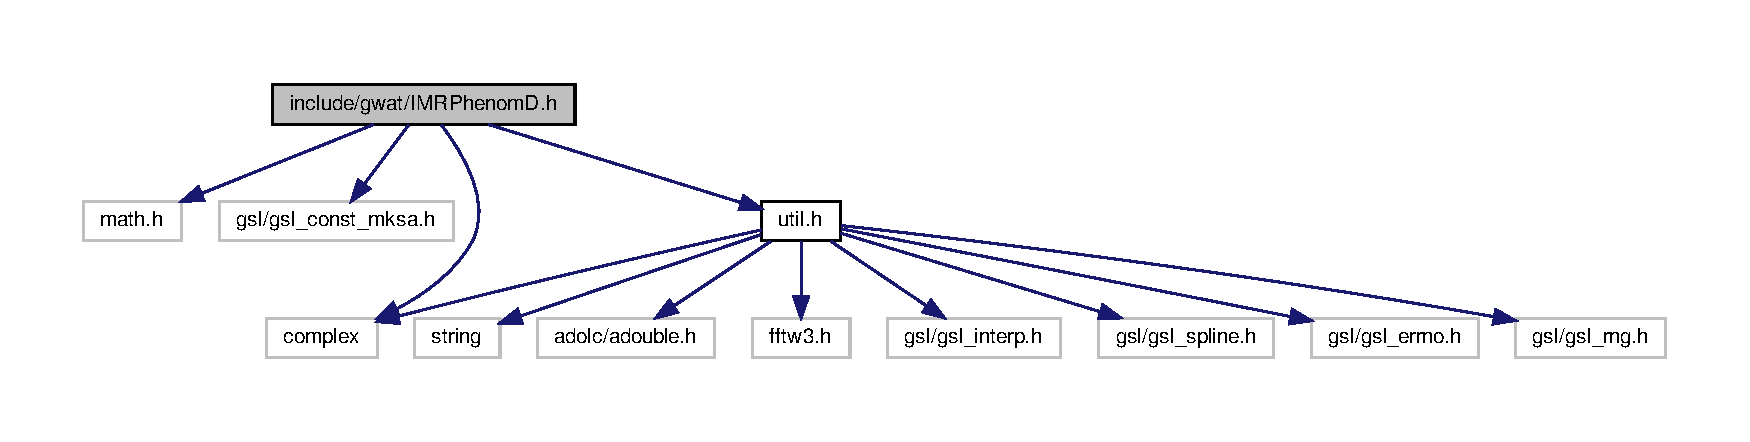
\includegraphics[width=350pt]{IMRPhenomD_8h__incl}
\end{center}
\end{figure}
This graph shows which files directly or indirectly include this file\+:
\nopagebreak
\begin{figure}[H]
\begin{center}
\leavevmode
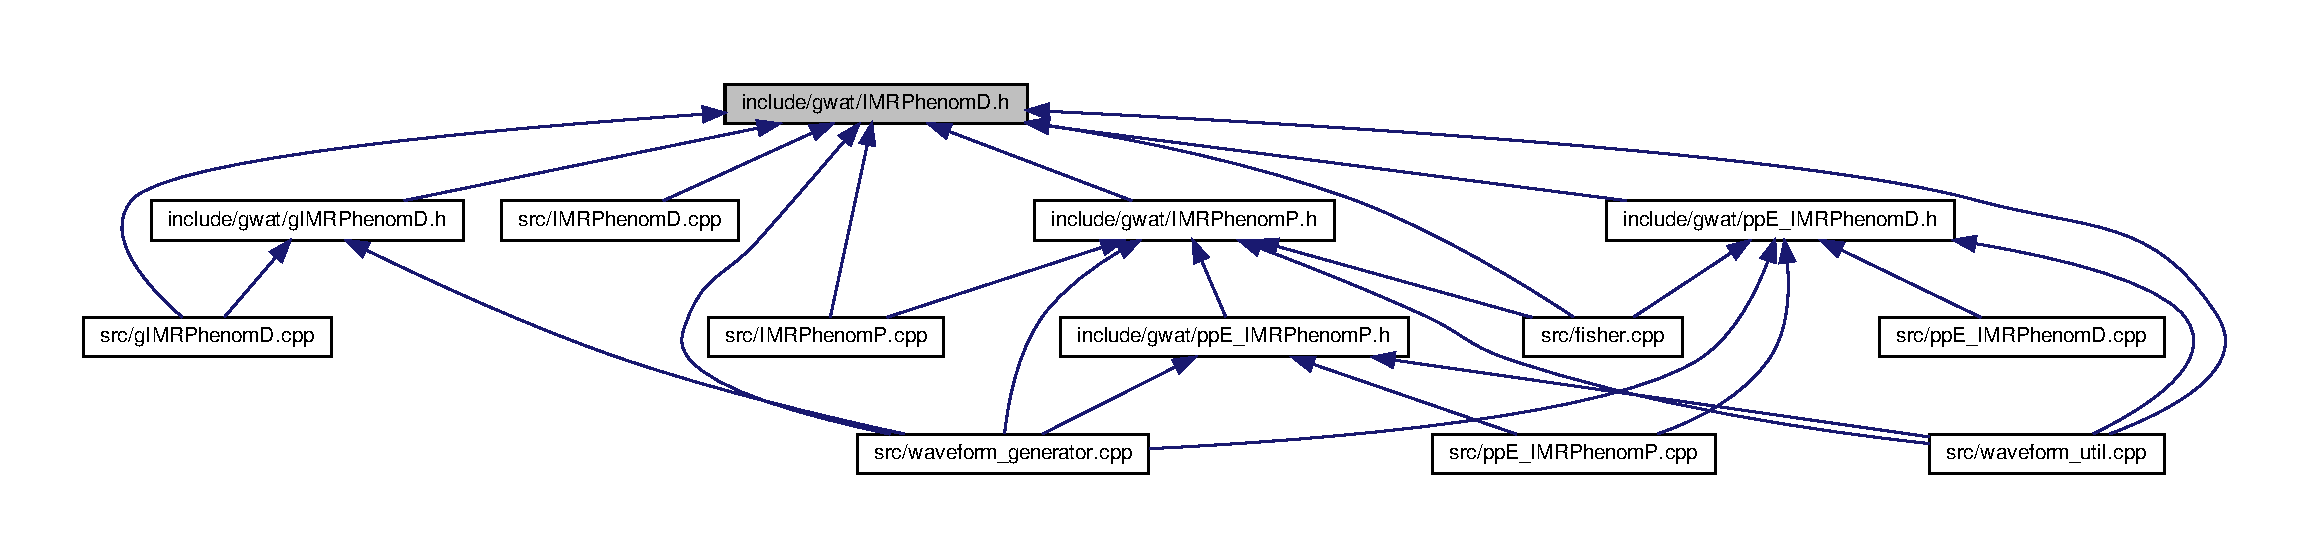
\includegraphics[width=350pt]{IMRPhenomD_8h__dep__incl}
\end{center}
\end{figure}
\doxysubsection*{Classes}
\begin{DoxyCompactItemize}
\item 
struct \mbox{\hyperlink{structlambda__parameters}{lambda\+\_\+parameters$<$ T $>$}}
\item 
class \mbox{\hyperlink{classIMRPhenomD}{I\+M\+R\+Phenom\+D$<$ T $>$}}
\end{DoxyCompactItemize}
\doxysubsection*{Variables}
\begin{DoxyCompactItemize}
\item 
const double \mbox{\hyperlink{IMRPhenomD_8h_ab4244995783dcaa1f99791db55aeb118}{lambda\+\_\+num\+\_\+params}} \mbox{[}19\mbox{]}\mbox{[}11\mbox{]}
\end{DoxyCompactItemize}


\doxysubsection{Detailed Description}
Header file for utilities 

\doxysubsection{Variable Documentation}
\mbox{\Hypertarget{IMRPhenomD_8h_ab4244995783dcaa1f99791db55aeb118}\label{IMRPhenomD_8h_ab4244995783dcaa1f99791db55aeb118}} 
\index{IMRPhenomD.h@{IMRPhenomD.h}!lambda\_num\_params@{lambda\_num\_params}}
\index{lambda\_num\_params@{lambda\_num\_params}!IMRPhenomD.h@{IMRPhenomD.h}}
\doxysubsubsection{\texorpdfstring{lambda\_num\_params}{lambda\_num\_params}}
{\footnotesize\ttfamily const double lambda\+\_\+num\+\_\+params\mbox{[}19\mbox{]}\mbox{[}11\mbox{]}}

Numerically calibrated parameters from ar\+Xiv\+:1508.\+07253 see the table in the data directory for labeled version from lalsuite 
\hypertarget{mcmc__routines_8h}{}\section{include/mcmc\+\_\+routines.h File Reference}
\label{mcmc__routines_8h}\index{include/mcmc\+\_\+routines.\+h@{include/mcmc\+\_\+routines.\+h}}
{\ttfamily \#include $<$complex$>$}\newline
{\ttfamily \#include $<$fftw3.\+h$>$}\newline
Include dependency graph for mcmc\+\_\+routines.\+h\+:\nopagebreak
\begin{figure}[H]
\begin{center}
\leavevmode
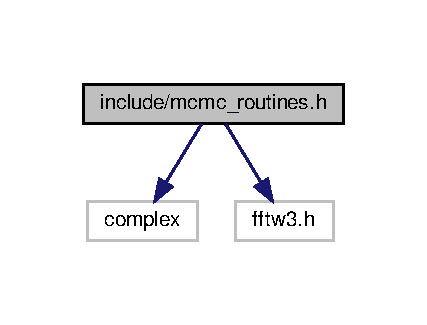
\includegraphics[width=205pt]{mcmc__routines_8h__incl}
\end{center}
\end{figure}
This graph shows which files directly or indirectly include this file\+:\nopagebreak
\begin{figure}[H]
\begin{center}
\leavevmode
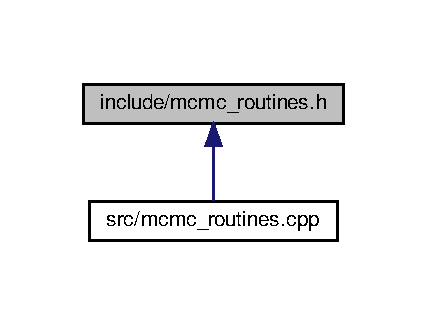
\includegraphics[width=205pt]{mcmc__routines_8h__dep__incl}
\end{center}
\end{figure}
\subsection*{Classes}
\begin{DoxyCompactItemize}
\item 
struct \hyperlink{structfftw__outline}{fftw\+\_\+outline}
\end{DoxyCompactItemize}
\subsection*{Functions}
\begin{DoxyCompactItemize}
\item 
double \hyperlink{mcmc__routines_8h_abd627450e43bf7ef683d875d804b7503}{maximized\+\_\+coal\+\_\+log\+\_\+likelihood\+\_\+\+I\+M\+R\+PhenomD} (double $\ast$frequencies, int length, std\+::complex$<$ double $>$ $\ast$data, double $\ast$noise, double S\+NR, double chirpmass, double symmetric\+\_\+mass\+\_\+ratio, double spin1, double spin2, bool N\+Sflag, \hyperlink{structfftw__outline}{fftw\+\_\+outline} $\ast$plan)
\begin{DoxyCompactList}\small\item\em Function to calculate the log Likelihood as defined by -\/1/2 (d-\/h$\vert$d-\/h) maximized over the extrinsic parameters phic and tc. \end{DoxyCompactList}\item 
double \hyperlink{mcmc__routines_8h_ae78896f8e8acd8dfaff6ff33a732284a}{maximized\+\_\+coal\+\_\+log\+\_\+likelihood\+\_\+\+I\+M\+R\+PhenomD} (double $\ast$frequencies, size\+\_\+t length, double $\ast$real\+\_\+data, double $\ast$imag\+\_\+data, double $\ast$noise, double S\+NR, double chirpmass, double symmetric\+\_\+mass\+\_\+ratio, double spin1, double spin2, bool N\+Sflag)
\item 
double \hyperlink{mcmc__routines_8h_a2635acb06ca0e448854aaab3fd7037c3}{maximized\+\_\+coal\+\_\+log\+\_\+likelihood\+\_\+\+I\+M\+R\+PhenomD} (double $\ast$frequencies, size\+\_\+t length, double $\ast$real\+\_\+data, double $\ast$imag\+\_\+data, double $\ast$noise, double S\+NR, double chirpmass, double symmetric\+\_\+mass\+\_\+ratio, double spin1, double spin2, bool N\+Sflag, \hyperlink{structfftw__outline}{fftw\+\_\+outline} $\ast$plan)
\item 
double \hyperlink{mcmc__routines_8h_ac66db6fc5c75ee33b84a48724b4738ef}{maximized\+\_\+coal\+\_\+log\+\_\+likelihood\+\_\+\+I\+M\+R\+Phenom\+D\+\_\+\+Full\+\_\+\+Param} (double $\ast$frequencies, int length, std\+::complex$<$ double $>$ $\ast$data, double $\ast$noise, double chirpmass, double symmetric\+\_\+mass\+\_\+ratio, double spin1, double spin2, double Luminosity\+\_\+\+Distance, double theta, double phi, double iota, bool N\+Sflag, \hyperlink{structfftw__outline}{fftw\+\_\+outline} $\ast$plan)
\item 
double \hyperlink{mcmc__routines_8h_a2322ab4b42380145e742ad564c643874}{maximized\+\_\+coal\+\_\+log\+\_\+likelihood\+\_\+\+I\+M\+R\+Phenom\+D\+\_\+\+Full\+\_\+\+Param} (double $\ast$frequencies, size\+\_\+t length, double $\ast$real\+\_\+data, double $\ast$imag\+\_\+data, double $\ast$noise, double chirpmass, double symmetric\+\_\+mass\+\_\+ratio, double spin1, double spin2, double Luminosity\+\_\+\+Distance, double theta, double phi, double iota, bool N\+Sflag)
\item 
double \hyperlink{mcmc__routines_8h_a3fbdbcf0651bad5541eb6e366c62de23}{maximized\+\_\+coal\+\_\+log\+\_\+likelihood\+\_\+\+I\+M\+R\+Phenom\+D\+\_\+\+Full\+\_\+\+Param} (double $\ast$frequencies, size\+\_\+t length, double $\ast$real\+\_\+data, double $\ast$imag\+\_\+data, double $\ast$noise, double chirpmass, double symmetric\+\_\+mass\+\_\+ratio, double spin1, double spin2, double Luminosity\+\_\+\+Distance, double theta, double phi, double iota, bool N\+Sflag, \hyperlink{structfftw__outline}{fftw\+\_\+outline} $\ast$plan)
\item 
\mbox{\Hypertarget{mcmc__routines_8h_a1599f89f2f16fbd3d5e95f87f48f88a0}\label{mcmc__routines_8h_a1599f89f2f16fbd3d5e95f87f48f88a0}} 
void {\bfseries initiate\+\_\+likelihood\+\_\+function} (\hyperlink{structfftw__outline}{fftw\+\_\+outline} $\ast$plan, int length)
\item 
\mbox{\Hypertarget{mcmc__routines_8h_a1433ee87cc1dd700874c1db0b1740d7c}\label{mcmc__routines_8h_a1433ee87cc1dd700874c1db0b1740d7c}} 
void {\bfseries deactivate\+\_\+likelihood\+\_\+function} (\hyperlink{structfftw__outline}{fftw\+\_\+outline} $\ast$plan)
\end{DoxyCompactItemize}


\subsection{Function Documentation}
\mbox{\Hypertarget{mcmc__routines_8h_abd627450e43bf7ef683d875d804b7503}\label{mcmc__routines_8h_abd627450e43bf7ef683d875d804b7503}} 
\index{mcmc\+\_\+routines.\+h@{mcmc\+\_\+routines.\+h}!maximized\+\_\+coal\+\_\+log\+\_\+likelihood\+\_\+\+I\+M\+R\+PhenomD@{maximized\+\_\+coal\+\_\+log\+\_\+likelihood\+\_\+\+I\+M\+R\+PhenomD}}
\index{maximized\+\_\+coal\+\_\+log\+\_\+likelihood\+\_\+\+I\+M\+R\+PhenomD@{maximized\+\_\+coal\+\_\+log\+\_\+likelihood\+\_\+\+I\+M\+R\+PhenomD}!mcmc\+\_\+routines.\+h@{mcmc\+\_\+routines.\+h}}
\subsubsection{\texorpdfstring{maximized\+\_\+coal\+\_\+log\+\_\+likelihood\+\_\+\+I\+M\+R\+Phenom\+D()}{maximized\_coal\_log\_likelihood\_IMRPhenomD()}\hspace{0.1cm}{\footnotesize\ttfamily [1/3]}}
{\footnotesize\ttfamily double maximized\+\_\+coal\+\_\+log\+\_\+likelihood\+\_\+\+I\+M\+R\+PhenomD (\begin{DoxyParamCaption}\item[{double $\ast$}]{frequencies,  }\item[{int}]{length,  }\item[{std\+::complex$<$ double $>$ $\ast$}]{data,  }\item[{double $\ast$}]{noise,  }\item[{double}]{S\+NR,  }\item[{double}]{chirpmass,  }\item[{double}]{symmetric\+\_\+mass\+\_\+ratio,  }\item[{double}]{spin1,  }\item[{double}]{spin2,  }\item[{bool}]{N\+Sflag,  }\item[{\hyperlink{structfftw__outline}{fftw\+\_\+outline} $\ast$}]{plan }\end{DoxyParamCaption})}



Function to calculate the log Likelihood as defined by -\/1/2 (d-\/h$\vert$d-\/h) maximized over the extrinsic parameters phic and tc. 

frequency array must be uniform spacing -\/ this shouldn\textquotesingle{}t be a problem when working with real data as D\+FT return uniform spacing 
\begin{DoxyParams}{Parameters}
{\em chirpmass} & in solar masses \\
\hline
\end{DoxyParams}
\mbox{\Hypertarget{mcmc__routines_8h_ae78896f8e8acd8dfaff6ff33a732284a}\label{mcmc__routines_8h_ae78896f8e8acd8dfaff6ff33a732284a}} 
\index{mcmc\+\_\+routines.\+h@{mcmc\+\_\+routines.\+h}!maximized\+\_\+coal\+\_\+log\+\_\+likelihood\+\_\+\+I\+M\+R\+PhenomD@{maximized\+\_\+coal\+\_\+log\+\_\+likelihood\+\_\+\+I\+M\+R\+PhenomD}}
\index{maximized\+\_\+coal\+\_\+log\+\_\+likelihood\+\_\+\+I\+M\+R\+PhenomD@{maximized\+\_\+coal\+\_\+log\+\_\+likelihood\+\_\+\+I\+M\+R\+PhenomD}!mcmc\+\_\+routines.\+h@{mcmc\+\_\+routines.\+h}}
\subsubsection{\texorpdfstring{maximized\+\_\+coal\+\_\+log\+\_\+likelihood\+\_\+\+I\+M\+R\+Phenom\+D()}{maximized\_coal\_log\_likelihood\_IMRPhenomD()}\hspace{0.1cm}{\footnotesize\ttfamily [2/3]}}
{\footnotesize\ttfamily double maximized\+\_\+coal\+\_\+log\+\_\+likelihood\+\_\+\+I\+M\+R\+PhenomD (\begin{DoxyParamCaption}\item[{double $\ast$}]{frequencies,  }\item[{size\+\_\+t}]{length,  }\item[{double $\ast$}]{real\+\_\+data,  }\item[{double $\ast$}]{imag\+\_\+data,  }\item[{double $\ast$}]{noise,  }\item[{double}]{S\+NR,  }\item[{double}]{chirpmass,  }\item[{double}]{symmetric\+\_\+mass\+\_\+ratio,  }\item[{double}]{spin1,  }\item[{double}]{spin2,  }\item[{bool}]{N\+Sflag }\end{DoxyParamCaption})}


\begin{DoxyParams}{Parameters}
{\em chirpmass} & in solar masses \\
\hline
\end{DoxyParams}
\mbox{\Hypertarget{mcmc__routines_8h_a2635acb06ca0e448854aaab3fd7037c3}\label{mcmc__routines_8h_a2635acb06ca0e448854aaab3fd7037c3}} 
\index{mcmc\+\_\+routines.\+h@{mcmc\+\_\+routines.\+h}!maximized\+\_\+coal\+\_\+log\+\_\+likelihood\+\_\+\+I\+M\+R\+PhenomD@{maximized\+\_\+coal\+\_\+log\+\_\+likelihood\+\_\+\+I\+M\+R\+PhenomD}}
\index{maximized\+\_\+coal\+\_\+log\+\_\+likelihood\+\_\+\+I\+M\+R\+PhenomD@{maximized\+\_\+coal\+\_\+log\+\_\+likelihood\+\_\+\+I\+M\+R\+PhenomD}!mcmc\+\_\+routines.\+h@{mcmc\+\_\+routines.\+h}}
\subsubsection{\texorpdfstring{maximized\+\_\+coal\+\_\+log\+\_\+likelihood\+\_\+\+I\+M\+R\+Phenom\+D()}{maximized\_coal\_log\_likelihood\_IMRPhenomD()}\hspace{0.1cm}{\footnotesize\ttfamily [3/3]}}
{\footnotesize\ttfamily double maximized\+\_\+coal\+\_\+log\+\_\+likelihood\+\_\+\+I\+M\+R\+PhenomD (\begin{DoxyParamCaption}\item[{double $\ast$}]{frequencies,  }\item[{size\+\_\+t}]{length,  }\item[{double $\ast$}]{real\+\_\+data,  }\item[{double $\ast$}]{imag\+\_\+data,  }\item[{double $\ast$}]{noise,  }\item[{double}]{S\+NR,  }\item[{double}]{chirpmass,  }\item[{double}]{symmetric\+\_\+mass\+\_\+ratio,  }\item[{double}]{spin1,  }\item[{double}]{spin2,  }\item[{bool}]{N\+Sflag,  }\item[{\hyperlink{structfftw__outline}{fftw\+\_\+outline} $\ast$}]{plan }\end{DoxyParamCaption})}


\begin{DoxyParams}{Parameters}
{\em chirpmass} & in solar masses \\
\hline
\end{DoxyParams}
\mbox{\Hypertarget{mcmc__routines_8h_ac66db6fc5c75ee33b84a48724b4738ef}\label{mcmc__routines_8h_ac66db6fc5c75ee33b84a48724b4738ef}} 
\index{mcmc\+\_\+routines.\+h@{mcmc\+\_\+routines.\+h}!maximized\+\_\+coal\+\_\+log\+\_\+likelihood\+\_\+\+I\+M\+R\+Phenom\+D\+\_\+\+Full\+\_\+\+Param@{maximized\+\_\+coal\+\_\+log\+\_\+likelihood\+\_\+\+I\+M\+R\+Phenom\+D\+\_\+\+Full\+\_\+\+Param}}
\index{maximized\+\_\+coal\+\_\+log\+\_\+likelihood\+\_\+\+I\+M\+R\+Phenom\+D\+\_\+\+Full\+\_\+\+Param@{maximized\+\_\+coal\+\_\+log\+\_\+likelihood\+\_\+\+I\+M\+R\+Phenom\+D\+\_\+\+Full\+\_\+\+Param}!mcmc\+\_\+routines.\+h@{mcmc\+\_\+routines.\+h}}
\subsubsection{\texorpdfstring{maximized\+\_\+coal\+\_\+log\+\_\+likelihood\+\_\+\+I\+M\+R\+Phenom\+D\+\_\+\+Full\+\_\+\+Param()}{maximized\_coal\_log\_likelihood\_IMRPhenomD\_Full\_Param()}\hspace{0.1cm}{\footnotesize\ttfamily [1/3]}}
{\footnotesize\ttfamily double maximized\+\_\+coal\+\_\+log\+\_\+likelihood\+\_\+\+I\+M\+R\+Phenom\+D\+\_\+\+Full\+\_\+\+Param (\begin{DoxyParamCaption}\item[{double $\ast$}]{frequencies,  }\item[{int}]{length,  }\item[{std\+::complex$<$ double $>$ $\ast$}]{data,  }\item[{double $\ast$}]{noise,  }\item[{double}]{chirpmass,  }\item[{double}]{symmetric\+\_\+mass\+\_\+ratio,  }\item[{double}]{spin1,  }\item[{double}]{spin2,  }\item[{double}]{Luminosity\+\_\+\+Distance,  }\item[{double}]{theta,  }\item[{double}]{phi,  }\item[{double}]{iota,  }\item[{bool}]{N\+Sflag,  }\item[{\hyperlink{structfftw__outline}{fftw\+\_\+outline} $\ast$}]{plan }\end{DoxyParamCaption})}


\begin{DoxyParams}{Parameters}
{\em chirpmass} & in solar masses \\
\hline
\end{DoxyParams}
\mbox{\Hypertarget{mcmc__routines_8h_a2322ab4b42380145e742ad564c643874}\label{mcmc__routines_8h_a2322ab4b42380145e742ad564c643874}} 
\index{mcmc\+\_\+routines.\+h@{mcmc\+\_\+routines.\+h}!maximized\+\_\+coal\+\_\+log\+\_\+likelihood\+\_\+\+I\+M\+R\+Phenom\+D\+\_\+\+Full\+\_\+\+Param@{maximized\+\_\+coal\+\_\+log\+\_\+likelihood\+\_\+\+I\+M\+R\+Phenom\+D\+\_\+\+Full\+\_\+\+Param}}
\index{maximized\+\_\+coal\+\_\+log\+\_\+likelihood\+\_\+\+I\+M\+R\+Phenom\+D\+\_\+\+Full\+\_\+\+Param@{maximized\+\_\+coal\+\_\+log\+\_\+likelihood\+\_\+\+I\+M\+R\+Phenom\+D\+\_\+\+Full\+\_\+\+Param}!mcmc\+\_\+routines.\+h@{mcmc\+\_\+routines.\+h}}
\subsubsection{\texorpdfstring{maximized\+\_\+coal\+\_\+log\+\_\+likelihood\+\_\+\+I\+M\+R\+Phenom\+D\+\_\+\+Full\+\_\+\+Param()}{maximized\_coal\_log\_likelihood\_IMRPhenomD\_Full\_Param()}\hspace{0.1cm}{\footnotesize\ttfamily [2/3]}}
{\footnotesize\ttfamily double maximized\+\_\+coal\+\_\+log\+\_\+likelihood\+\_\+\+I\+M\+R\+Phenom\+D\+\_\+\+Full\+\_\+\+Param (\begin{DoxyParamCaption}\item[{double $\ast$}]{frequencies,  }\item[{size\+\_\+t}]{length,  }\item[{double $\ast$}]{real\+\_\+data,  }\item[{double $\ast$}]{imag\+\_\+data,  }\item[{double $\ast$}]{noise,  }\item[{double}]{chirpmass,  }\item[{double}]{symmetric\+\_\+mass\+\_\+ratio,  }\item[{double}]{spin1,  }\item[{double}]{spin2,  }\item[{double}]{Luminosity\+\_\+\+Distance,  }\item[{double}]{theta,  }\item[{double}]{phi,  }\item[{double}]{iota,  }\item[{bool}]{N\+Sflag }\end{DoxyParamCaption})}


\begin{DoxyParams}{Parameters}
{\em chirpmass} & in solar masses \\
\hline
\end{DoxyParams}
\mbox{\Hypertarget{mcmc__routines_8h_a3fbdbcf0651bad5541eb6e366c62de23}\label{mcmc__routines_8h_a3fbdbcf0651bad5541eb6e366c62de23}} 
\index{mcmc\+\_\+routines.\+h@{mcmc\+\_\+routines.\+h}!maximized\+\_\+coal\+\_\+log\+\_\+likelihood\+\_\+\+I\+M\+R\+Phenom\+D\+\_\+\+Full\+\_\+\+Param@{maximized\+\_\+coal\+\_\+log\+\_\+likelihood\+\_\+\+I\+M\+R\+Phenom\+D\+\_\+\+Full\+\_\+\+Param}}
\index{maximized\+\_\+coal\+\_\+log\+\_\+likelihood\+\_\+\+I\+M\+R\+Phenom\+D\+\_\+\+Full\+\_\+\+Param@{maximized\+\_\+coal\+\_\+log\+\_\+likelihood\+\_\+\+I\+M\+R\+Phenom\+D\+\_\+\+Full\+\_\+\+Param}!mcmc\+\_\+routines.\+h@{mcmc\+\_\+routines.\+h}}
\subsubsection{\texorpdfstring{maximized\+\_\+coal\+\_\+log\+\_\+likelihood\+\_\+\+I\+M\+R\+Phenom\+D\+\_\+\+Full\+\_\+\+Param()}{maximized\_coal\_log\_likelihood\_IMRPhenomD\_Full\_Param()}\hspace{0.1cm}{\footnotesize\ttfamily [3/3]}}
{\footnotesize\ttfamily double maximized\+\_\+coal\+\_\+log\+\_\+likelihood\+\_\+\+I\+M\+R\+Phenom\+D\+\_\+\+Full\+\_\+\+Param (\begin{DoxyParamCaption}\item[{double $\ast$}]{frequencies,  }\item[{size\+\_\+t}]{length,  }\item[{double $\ast$}]{real\+\_\+data,  }\item[{double $\ast$}]{imag\+\_\+data,  }\item[{double $\ast$}]{noise,  }\item[{double}]{chirpmass,  }\item[{double}]{symmetric\+\_\+mass\+\_\+ratio,  }\item[{double}]{spin1,  }\item[{double}]{spin2,  }\item[{double}]{Luminosity\+\_\+\+Distance,  }\item[{double}]{theta,  }\item[{double}]{phi,  }\item[{double}]{iota,  }\item[{bool}]{N\+Sflag,  }\item[{\hyperlink{structfftw__outline}{fftw\+\_\+outline} $\ast$}]{plan }\end{DoxyParamCaption})}


\begin{DoxyParams}{Parameters}
{\em chirpmass} & in solar masses \\
\hline
\end{DoxyParams}

\hypertarget{noise__util_8h}{}\section{include/noise\+\_\+util.h File Reference}
\label{noise__util_8h}\index{include/noise\+\_\+util.\+h@{include/noise\+\_\+util.\+h}}
{\ttfamily \#include $<$string$>$}\newline
Include dependency graph for noise\+\_\+util.\+h\+:\nopagebreak
\begin{figure}[H]
\begin{center}
\leavevmode
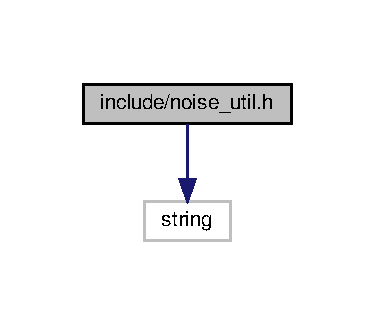
\includegraphics[width=180pt]{noise__util_8h__incl}
\end{center}
\end{figure}
This graph shows which files directly or indirectly include this file\+:\nopagebreak
\begin{figure}[H]
\begin{center}
\leavevmode
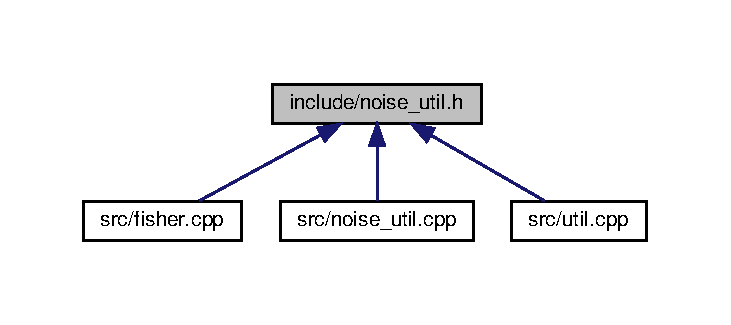
\includegraphics[width=350pt]{noise__util_8h__dep__incl}
\end{center}
\end{figure}
\subsection*{Functions}
\begin{DoxyCompactItemize}
\item 
void \hyperlink{noise__util_8h_a551c603f441283ca3fe5d415d47bdc4d}{populate\+\_\+noise} (double $\ast$frequencies, std\+::string detector, double $\ast$noise\+\_\+root, int length=0)
\begin{DoxyCompactList}\small\item\em Function to populate the squareroot of the noise curve for various detectors. \end{DoxyCompactList}\item 
\mbox{\Hypertarget{noise__util_8h_a6e657285283899f91aa3b7ec7963c120}\label{noise__util_8h_a6e657285283899f91aa3b7ec7963c120}} 
double {\bfseries a\+L\+I\+G\+O\+\_\+analytic} (double f)
\item 
\mbox{\Hypertarget{noise__util_8h_a2e29bfa3018d037af4d1b52cabe47d39}\label{noise__util_8h_a2e29bfa3018d037af4d1b52cabe47d39}} 
double {\bfseries Hanford\+\_\+\+O1\+\_\+fitted} (double f)
\end{DoxyCompactItemize}


\subsection{Function Documentation}
\mbox{\Hypertarget{noise__util_8h_a551c603f441283ca3fe5d415d47bdc4d}\label{noise__util_8h_a551c603f441283ca3fe5d415d47bdc4d}} 
\index{noise\+\_\+util.\+h@{noise\+\_\+util.\+h}!populate\+\_\+noise@{populate\+\_\+noise}}
\index{populate\+\_\+noise@{populate\+\_\+noise}!noise\+\_\+util.\+h@{noise\+\_\+util.\+h}}
\subsubsection{\texorpdfstring{populate\+\_\+noise()}{populate\_noise()}}
{\footnotesize\ttfamily void populate\+\_\+noise (\begin{DoxyParamCaption}\item[{double $\ast$}]{frequencies,  }\item[{std\+::string}]{detector,  }\item[{double $\ast$}]{noise\+\_\+root,  }\item[{int}]{length }\end{DoxyParamCaption})}



Function to populate the squareroot of the noise curve for various detectors. 

If frequencies are left as N\+U\+LL, standard frequency spacing is applied and the frequencies are returned, in which case the frequencies argument becomes an output array

Detector names must be spelled exactly

Detectors include\+: a\+L\+I\+G\+O\+\_\+analytic, Hanford\+\_\+\+O1\+\_\+fitted 
\begin{DoxyParams}{Parameters}
{\em frequencies} & double array of frquencies (N\+U\+LL) \\
\hline
{\em detector} & String to designate the detector noise curve to be used \\
\hline
{\em noise\+\_\+root} & ouptput double array for the square root of the P\+SD of the noise of the specified detector \\
\hline
{\em length} & integer length of the output and input arrays \\
\hline
\end{DoxyParams}

\hypertarget{ppE__IMRPhenomD_8h}{}\doxysection{include/gwat/pp\+E\+\_\+\+I\+M\+R\+PhenomD.h File Reference}
\label{ppE__IMRPhenomD_8h}\index{include/gwat/ppE\_IMRPhenomD.h@{include/gwat/ppE\_IMRPhenomD.h}}
{\ttfamily \#include \char`\"{}I\+M\+R\+Phenom\+D.\+h\char`\"{}}\newline
{\ttfamily \#include \char`\"{}util.\+h\char`\"{}}\newline
Include dependency graph for pp\+E\+\_\+\+I\+M\+R\+Phenom\+D.\+h\+:
% FIG 0
This graph shows which files directly or indirectly include this file\+:
% FIG 1
\doxysubsection*{Classes}
\begin{DoxyCompactItemize}
\item 
class \mbox{\hyperlink{classppE__IMRPhenomD__Inspiral}{pp\+E\+\_\+\+I\+M\+R\+Phenom\+D\+\_\+\+Inspiral$<$ T $>$}}
\item 
class \mbox{\hyperlink{classppE__IMRPhenomD__IMR}{pp\+E\+\_\+\+I\+M\+R\+Phenom\+D\+\_\+\+I\+M\+R$<$ T $>$}}
\item 
class \mbox{\hyperlink{classdCS__IMRPhenomD__log}{d\+C\+S\+\_\+\+I\+M\+R\+Phenom\+D\+\_\+log$<$ T $>$}}
\item 
class \mbox{\hyperlink{classdCS__IMRPhenomD}{d\+C\+S\+\_\+\+I\+M\+R\+Phenom\+D$<$ T $>$}}
\item 
class \mbox{\hyperlink{classEdGB__IMRPhenomD__log}{Ed\+G\+B\+\_\+\+I\+M\+R\+Phenom\+D\+\_\+log$<$ T $>$}}
\item 
class \mbox{\hyperlink{classEdGB__IMRPhenomD}{Ed\+G\+B\+\_\+\+I\+M\+R\+Phenom\+D$<$ T $>$}}
\end{DoxyCompactItemize}

\hypertarget{util_8h}{}\section{include/util.h File Reference}
\label{util_8h}\index{include/util.\+h@{include/util.\+h}}
{\ttfamily \#include $<$string$>$}\newline
{\ttfamily \#include $<$complex$>$}\newline
{\ttfamily \#include $<$adolc/adouble.\+h$>$}\newline
Include dependency graph for util.\+h\+:\nopagebreak
\begin{figure}[H]
\begin{center}
\leavevmode
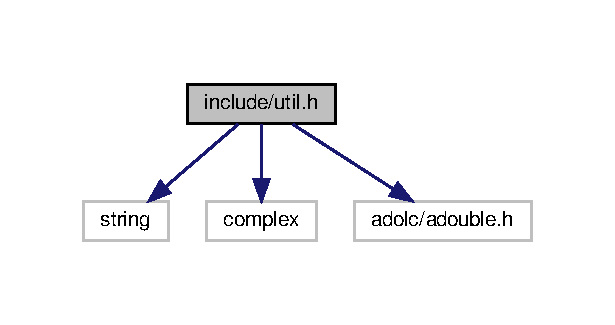
\includegraphics[width=295pt]{util_8h__incl}
\end{center}
\end{figure}
This graph shows which files directly or indirectly include this file\+:\nopagebreak
\begin{figure}[H]
\begin{center}
\leavevmode
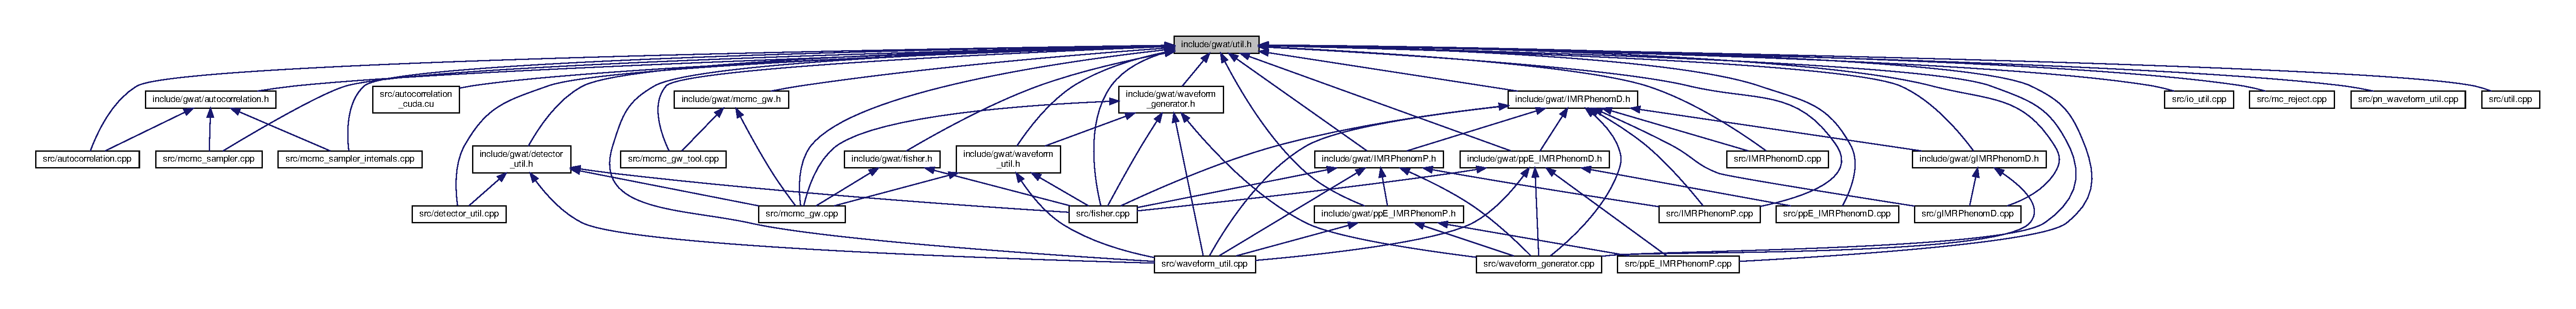
\includegraphics[width=350pt]{util_8h__dep__incl}
\end{center}
\end{figure}
\subsection*{Classes}
\begin{DoxyCompactItemize}
\item 
struct \hyperlink{structgen__params}{gen\+\_\+params}
\item 
struct \hyperlink{structuseful__powers}{useful\+\_\+powers$<$ T $>$}
\begin{DoxyCompactList}\small\item\em To speed up calculations within the for loops, we pre-\/calculate reoccuring powers of M$\ast$F and Pi, since the pow() function is prohibatively slow. \end{DoxyCompactList}\item 
struct \hyperlink{structsource__parameters}{source\+\_\+parameters$<$ T $>$}
\end{DoxyCompactItemize}
\subsection*{Functions}
\begin{DoxyCompactItemize}
\item 
\mbox{\Hypertarget{util_8h_a06ffbad5fe4daa3872db626f90556202}\label{util_8h_a06ffbad5fe4daa3872db626f90556202}} 
double \hyperlink{util_8h_a06ffbad5fe4daa3872db626f90556202}{calculate\+\_\+eta} (double mass1, double mass2)
\begin{DoxyCompactList}\small\item\em Calculates the symmetric mass ration from the two component masses. \end{DoxyCompactList}\item 
\mbox{\Hypertarget{util_8h_adc4391c722f94cb17f0e0275a0930fa9}\label{util_8h_adc4391c722f94cb17f0e0275a0930fa9}} 
adouble {\bfseries calculate\+\_\+eta} (adouble mass1, adouble mass2)
\item 
double \hyperlink{util_8h_af7aeeebcf190ab70c667a478a51ce435}{calculate\+\_\+chirpmass} (double mass1, double mass2)
\begin{DoxyCompactList}\small\item\em Calculates the chirp mass from the two component masses. \end{DoxyCompactList}\item 
\mbox{\Hypertarget{util_8h_a0a7a0da86013d639bf8689c9a01d8583}\label{util_8h_a0a7a0da86013d639bf8689c9a01d8583}} 
adouble {\bfseries calculate\+\_\+chirpmass} (adouble mass1, adouble mass2)
\item 
double \hyperlink{util_8h_a85a0fc50a6f06dd519a18a6d273a0b4a}{calculate\+\_\+mass1} (double chirpmass, double eta)
\begin{DoxyCompactList}\small\item\em Calculates the larger mass given a chirp mass and symmetric mass ratio. \end{DoxyCompactList}\item 
\mbox{\Hypertarget{util_8h_a663f11702648d9a84c9b573e9ab76f09}\label{util_8h_a663f11702648d9a84c9b573e9ab76f09}} 
adouble {\bfseries calculate\+\_\+mass1} (adouble chirpmass, adouble eta)
\item 
double \hyperlink{util_8h_a5f62f4a7c1011180080d72e0032cef1b}{calculate\+\_\+mass2} (double chirpmass, double eta)
\begin{DoxyCompactList}\small\item\em Calculates the smaller mass given a chirp mass and symmetric mass ratio. \end{DoxyCompactList}\item 
\mbox{\Hypertarget{util_8h_adb85ce9fbb2e3a438dd41a35c38a3237}\label{util_8h_adb85ce9fbb2e3a438dd41a35c38a3237}} 
adouble {\bfseries calculate\+\_\+mass2} (adouble chirpmass, adouble eta)
\item 
{\footnotesize template$<$class T $>$ }\\T \hyperlink{util_8h_a185f5ce6420f94f03d77915d94b06f4f}{trapezoidal\+\_\+sum\+\_\+uniform} (double delta\+\_\+x, int length, T $\ast$integrand)
\begin{DoxyCompactList}\small\item\em Trapezoidal sum rule to approximate discrete integral -\/ Uniform spacing. \end{DoxyCompactList}\item 
{\footnotesize template$<$class T $>$ }\\T \hyperlink{util_8h_ab7d3ff0c020ec0ffbe56f4271f425d68}{trapezoidal\+\_\+sum} (double $\ast$delta\+\_\+x, int length, T $\ast$integrand)
\begin{DoxyCompactList}\small\item\em Trapezoidal sum rule to approximate discrete integral -\/ Non-\/\+Uniform spacing. \end{DoxyCompactList}\item 
{\footnotesize template$<$class T $>$ }\\T \hyperlink{util_8h_ad77170ec9220ef33a32f2540e9184e31}{simpsons\+\_\+sum} (double delta\+\_\+x, int length, T $\ast$integrand)
\begin{DoxyCompactList}\small\item\em Simpsons sum rule to approximate discrete integral -\/ Uniform spacing. \end{DoxyCompactList}\item 
\mbox{\Hypertarget{util_8h_ae40cc3f267c33745a8a2485638d5db55}\label{util_8h_ae40cc3f267c33745a8a2485638d5db55}} 
long {\bfseries factorial} (long num)
\end{DoxyCompactItemize}
\subsection*{Variables}
\begin{DoxyCompactItemize}
\item 
const double \hyperlink{util_8h_ae35ccfea47f0da0a31cf1d13c80f3c58}{gamma\+\_\+E} = 0.\+5772156649015328606065120900824024310421
\item 
const double \hyperlink{util_8h_a8fc6defe4e499b1b9b9c275689e44352}{c} = 299792458.
\item 
const double \hyperlink{util_8h_ab97e4616d23ed4c2961295010c1afc3c}{G} =6.\+674e-\/11$\ast$(1.\+98855e30)
\item 
const double \hyperlink{util_8h_a498f9210d23417e309c01ad5cb9a635b}{M\+S\+O\+L\+\_\+\+S\+EC} =492549095.e-\/14
\item 
const double \hyperlink{util_8h_a47be806b6c8a58bd030f167ca91ed201}{M\+P\+C\+\_\+\+S\+EC} = 3085677581.e13/\hyperlink{util_8h_a8fc6defe4e499b1b9b9c275689e44352}{c}
\end{DoxyCompactItemize}


\subsection{Detailed Description}
General utilities (functions and structures) independent of modelling method 

\subsection{Function Documentation}
\mbox{\Hypertarget{util_8h_af7aeeebcf190ab70c667a478a51ce435}\label{util_8h_af7aeeebcf190ab70c667a478a51ce435}} 
\index{util.\+h@{util.\+h}!calculate\+\_\+chirpmass@{calculate\+\_\+chirpmass}}
\index{calculate\+\_\+chirpmass@{calculate\+\_\+chirpmass}!util.\+h@{util.\+h}}
\subsubsection{\texorpdfstring{calculate\+\_\+chirpmass()}{calculate\_chirpmass()}}
{\footnotesize\ttfamily double calculate\+\_\+chirpmass (\begin{DoxyParamCaption}\item[{double}]{mass1,  }\item[{double}]{mass2 }\end{DoxyParamCaption})}



Calculates the chirp mass from the two component masses. 

The output units are whatever units the input masses are \mbox{\Hypertarget{util_8h_a85a0fc50a6f06dd519a18a6d273a0b4a}\label{util_8h_a85a0fc50a6f06dd519a18a6d273a0b4a}} 
\index{util.\+h@{util.\+h}!calculate\+\_\+mass1@{calculate\+\_\+mass1}}
\index{calculate\+\_\+mass1@{calculate\+\_\+mass1}!util.\+h@{util.\+h}}
\subsubsection{\texorpdfstring{calculate\+\_\+mass1()}{calculate\_mass1()}}
{\footnotesize\ttfamily double calculate\+\_\+mass1 (\begin{DoxyParamCaption}\item[{double}]{chirpmass,  }\item[{double}]{eta }\end{DoxyParamCaption})}



Calculates the larger mass given a chirp mass and symmetric mass ratio. 

Units of the output match the units of the input chirp mass \mbox{\Hypertarget{util_8h_a5f62f4a7c1011180080d72e0032cef1b}\label{util_8h_a5f62f4a7c1011180080d72e0032cef1b}} 
\index{util.\+h@{util.\+h}!calculate\+\_\+mass2@{calculate\+\_\+mass2}}
\index{calculate\+\_\+mass2@{calculate\+\_\+mass2}!util.\+h@{util.\+h}}
\subsubsection{\texorpdfstring{calculate\+\_\+mass2()}{calculate\_mass2()}}
{\footnotesize\ttfamily double calculate\+\_\+mass2 (\begin{DoxyParamCaption}\item[{double}]{chirpmass,  }\item[{double}]{eta }\end{DoxyParamCaption})}



Calculates the smaller mass given a chirp mass and symmetric mass ratio. 

Units of the output match the units of the input chirp mass \mbox{\Hypertarget{util_8h_ad77170ec9220ef33a32f2540e9184e31}\label{util_8h_ad77170ec9220ef33a32f2540e9184e31}} 
\index{util.\+h@{util.\+h}!simpsons\+\_\+sum@{simpsons\+\_\+sum}}
\index{simpsons\+\_\+sum@{simpsons\+\_\+sum}!util.\+h@{util.\+h}}
\subsubsection{\texorpdfstring{simpsons\+\_\+sum()}{simpsons\_sum()}}
{\footnotesize\ttfamily template$<$class T $>$ \\
T simpsons\+\_\+sum (\begin{DoxyParamCaption}\item[{double}]{delta\+\_\+x,  }\item[{int}]{length,  }\item[{T $\ast$}]{integrand }\end{DoxyParamCaption})}



Simpsons sum rule to approximate discrete integral -\/ Uniform spacing. 

More accurate than the trapezoidal rule, but must be uniform \mbox{\Hypertarget{util_8h_ab7d3ff0c020ec0ffbe56f4271f425d68}\label{util_8h_ab7d3ff0c020ec0ffbe56f4271f425d68}} 
\index{util.\+h@{util.\+h}!trapezoidal\+\_\+sum@{trapezoidal\+\_\+sum}}
\index{trapezoidal\+\_\+sum@{trapezoidal\+\_\+sum}!util.\+h@{util.\+h}}
\subsubsection{\texorpdfstring{trapezoidal\+\_\+sum()}{trapezoidal\_sum()}}
{\footnotesize\ttfamily template$<$class T $>$ \\
T trapezoidal\+\_\+sum (\begin{DoxyParamCaption}\item[{double $\ast$}]{delta\+\_\+x,  }\item[{int}]{length,  }\item[{T $\ast$}]{integrand }\end{DoxyParamCaption})}



Trapezoidal sum rule to approximate discrete integral -\/ Non-\/\+Uniform spacing. 

This version is slower than the uniform version, but will handle non-\/uniform spacing \mbox{\Hypertarget{util_8h_a185f5ce6420f94f03d77915d94b06f4f}\label{util_8h_a185f5ce6420f94f03d77915d94b06f4f}} 
\index{util.\+h@{util.\+h}!trapezoidal\+\_\+sum\+\_\+uniform@{trapezoidal\+\_\+sum\+\_\+uniform}}
\index{trapezoidal\+\_\+sum\+\_\+uniform@{trapezoidal\+\_\+sum\+\_\+uniform}!util.\+h@{util.\+h}}
\subsubsection{\texorpdfstring{trapezoidal\+\_\+sum\+\_\+uniform()}{trapezoidal\_sum\_uniform()}}
{\footnotesize\ttfamily template$<$class T $>$ \\
T trapezoidal\+\_\+sum\+\_\+uniform (\begin{DoxyParamCaption}\item[{double}]{delta\+\_\+x,  }\item[{int}]{length,  }\item[{T $\ast$}]{integrand }\end{DoxyParamCaption})}



Trapezoidal sum rule to approximate discrete integral -\/ Uniform spacing. 

This version is faster than the general version, as it has half the function calls

Something may be wrong with this function -\/ had an overall offset for real data that was fixed by using the simpsons rule -\/ not sure if this was because of a boost in accuracy or because something is off with the trapezoidal sum 

\subsection{Variable Documentation}
\mbox{\Hypertarget{util_8h_a8fc6defe4e499b1b9b9c275689e44352}\label{util_8h_a8fc6defe4e499b1b9b9c275689e44352}} 
\index{util.\+h@{util.\+h}!c@{c}}
\index{c@{c}!util.\+h@{util.\+h}}
\subsubsection{\texorpdfstring{c}{c}}
{\footnotesize\ttfamily const double c = 299792458.}

Speed of light m/s \mbox{\Hypertarget{util_8h_ab97e4616d23ed4c2961295010c1afc3c}\label{util_8h_ab97e4616d23ed4c2961295010c1afc3c}} 
\index{util.\+h@{util.\+h}!G@{G}}
\index{G@{G}!util.\+h@{util.\+h}}
\subsubsection{\texorpdfstring{G}{G}}
{\footnotesize\ttfamily const double G =6.\+674e-\/11$\ast$(1.\+98855e30)}

Gravitational constant in m$\ast$$\ast$3/(s$\ast$$\ast$2 Sol\+Mass) \mbox{\Hypertarget{util_8h_ae35ccfea47f0da0a31cf1d13c80f3c58}\label{util_8h_ae35ccfea47f0da0a31cf1d13c80f3c58}} 
\index{util.\+h@{util.\+h}!gamma\+\_\+E@{gamma\+\_\+E}}
\index{gamma\+\_\+E@{gamma\+\_\+E}!util.\+h@{util.\+h}}
\subsubsection{\texorpdfstring{gamma\+\_\+E}{gamma\_E}}
{\footnotesize\ttfamily const double gamma\+\_\+E = 0.\+5772156649015328606065120900824024310421}

Euler number \mbox{\Hypertarget{util_8h_a47be806b6c8a58bd030f167ca91ed201}\label{util_8h_a47be806b6c8a58bd030f167ca91ed201}} 
\index{util.\+h@{util.\+h}!M\+P\+C\+\_\+\+S\+EC@{M\+P\+C\+\_\+\+S\+EC}}
\index{M\+P\+C\+\_\+\+S\+EC@{M\+P\+C\+\_\+\+S\+EC}!util.\+h@{util.\+h}}
\subsubsection{\texorpdfstring{M\+P\+C\+\_\+\+S\+EC}{MPC\_SEC}}
{\footnotesize\ttfamily const double M\+P\+C\+\_\+\+S\+EC = 3085677581.e13/\hyperlink{util_8h_a8fc6defe4e499b1b9b9c275689e44352}{c}}

consts.\+kpc.\+to(\textquotesingle{}m\textquotesingle{})$\ast$1000/c Mpc in sec \mbox{\Hypertarget{util_8h_a498f9210d23417e309c01ad5cb9a635b}\label{util_8h_a498f9210d23417e309c01ad5cb9a635b}} 
\index{util.\+h@{util.\+h}!M\+S\+O\+L\+\_\+\+S\+EC@{M\+S\+O\+L\+\_\+\+S\+EC}}
\index{M\+S\+O\+L\+\_\+\+S\+EC@{M\+S\+O\+L\+\_\+\+S\+EC}!util.\+h@{util.\+h}}
\subsubsection{\texorpdfstring{M\+S\+O\+L\+\_\+\+S\+EC}{MSOL\_SEC}}
{\footnotesize\ttfamily const double M\+S\+O\+L\+\_\+\+S\+EC =492549095.e-\/14}

G/c$\ast$$\ast$3 seconds per solar mass 
\hypertarget{waveform__generator_8h}{}\doxysection{include/gwat/waveform\+\_\+generator.h File Reference}
\label{waveform__generator_8h}\index{include/gwat/waveform\_generator.h@{include/gwat/waveform\_generator.h}}
{\ttfamily \#include $<$math.\+h$>$}\newline
{\ttfamily \#include \char`\"{}util.\+h\char`\"{}}\newline
{\ttfamily \#include $<$complex$>$}\newline
{\ttfamily \#include $<$string$>$}\newline
Include dependency graph for waveform\+\_\+generator.\+h\+:
\nopagebreak
\begin{figure}[H]
\begin{center}
\leavevmode
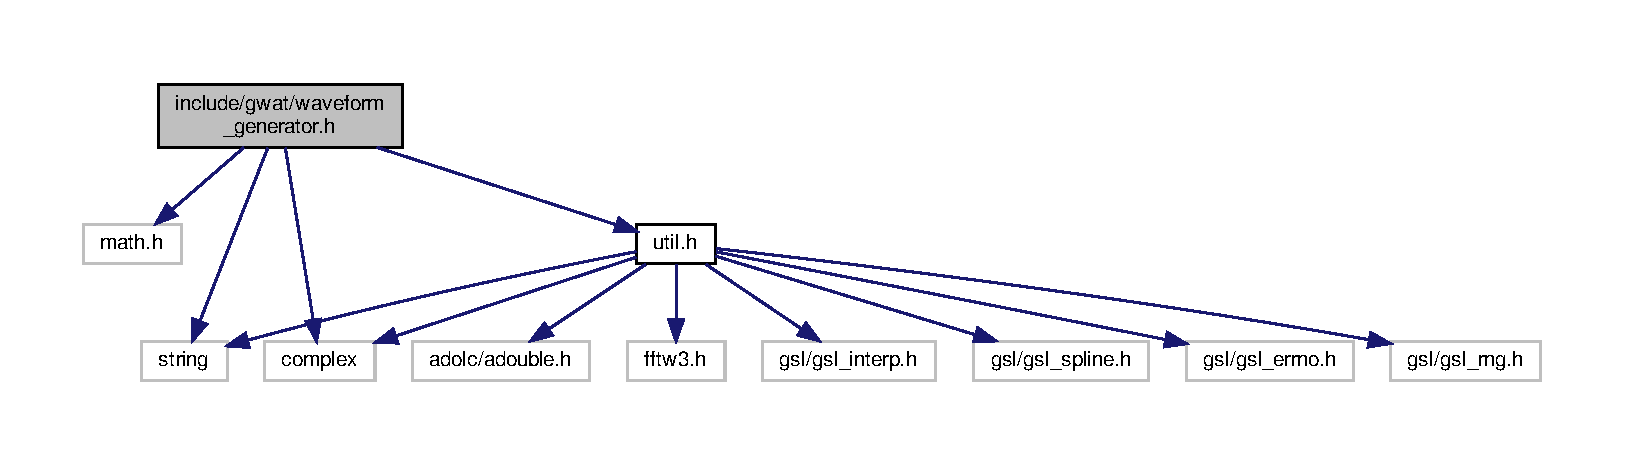
\includegraphics[width=350pt]{waveform__generator_8h__incl}
\end{center}
\end{figure}
This graph shows which files directly or indirectly include this file\+:
\nopagebreak
\begin{figure}[H]
\begin{center}
\leavevmode
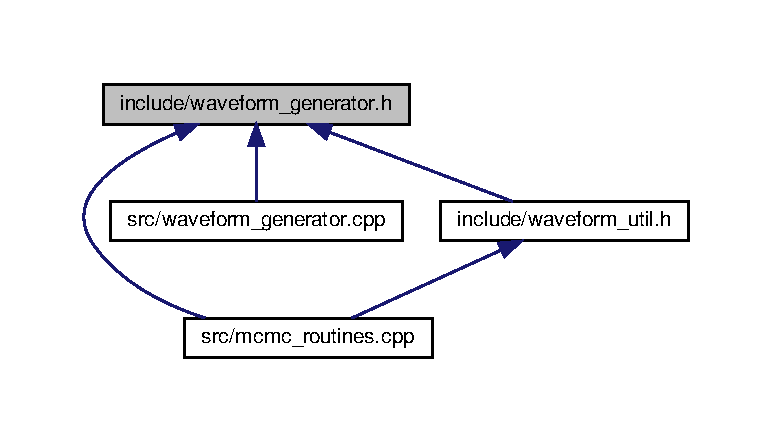
\includegraphics[width=350pt]{waveform__generator_8h__dep__incl}
\end{center}
\end{figure}
\doxysubsection*{Functions}
\begin{DoxyCompactItemize}
\item 
\mbox{\Hypertarget{waveform__generator_8h_a06574718b86529ab0480a6a673ada3f6}\label{waveform__generator_8h_a06574718b86529ab0480a6a673ada3f6}} 
{\footnotesize template$<$class T $>$ }\\int {\bfseries fourier\+\_\+waveform} (T $\ast$frequencies, int length, std\+::complex$<$ T $>$ $\ast$waveform\+\_\+plus, std\+::complex$<$ T $>$ $\ast$waveform\+\_\+cross, std\+::string generation\+\_\+method, \mbox{\hyperlink{classgen__params__base}{gen\+\_\+params\+\_\+base}}$<$ T $>$ $\ast$parameters)
\item 
\mbox{\Hypertarget{waveform__generator_8h_aab7ecf30458b3577aa1391c464bbe671}\label{waveform__generator_8h_aab7ecf30458b3577aa1391c464bbe671}} 
int {\bfseries fourier\+\_\+waveform} (double $\ast$frequencies, int length, double $\ast$waveform\+\_\+plus\+\_\+real, double $\ast$waveform\+\_\+plus\+\_\+imag, double $\ast$waveform\+\_\+cross\+\_\+real, double $\ast$waveform\+\_\+cross\+\_\+imag, std\+::string generation\+\_\+method, \mbox{\hyperlink{classgen__params}{gen\+\_\+params}} $\ast$parameters)
\item 
\mbox{\Hypertarget{waveform__generator_8h_ace521e7a8e3747632121ceabf6eaa305}\label{waveform__generator_8h_ace521e7a8e3747632121ceabf6eaa305}} 
int {\bfseries fourier\+\_\+waveform} (double $\ast$frequencies, int length, std\+::complex$<$ double $>$ $\ast$waveform, std\+::string generation\+\_\+method, \mbox{\hyperlink{classgen__params}{gen\+\_\+params}} $\ast$parameters)
\item 
\mbox{\Hypertarget{waveform__generator_8h_a3f551caee9adc33674e4b74daa6bbb54}\label{waveform__generator_8h_a3f551caee9adc33674e4b74daa6bbb54}} 
int {\bfseries fourier\+\_\+waveform} (double $\ast$frequencies, int length, double $\ast$waveform\+\_\+real, double $\ast$waveform\+\_\+imag, std\+::string generation\+\_\+method, \mbox{\hyperlink{classgen__params}{gen\+\_\+params}} $\ast$parameters)
\item 
\mbox{\Hypertarget{waveform__generator_8h_a0c791c00bc1552f2f70cadfbdff73a06}\label{waveform__generator_8h_a0c791c00bc1552f2f70cadfbdff73a06}} 
{\footnotesize template$<$class T $>$ }\\int {\bfseries fourier\+\_\+amplitude} (T $\ast$frequencies, int length, T $\ast$amplitude, std\+::string generation\+\_\+method, \mbox{\hyperlink{classgen__params__base}{gen\+\_\+params\+\_\+base}}$<$ T $>$ $\ast$parameters)
\item 
\mbox{\Hypertarget{waveform__generator_8h_a68aef1d43c5333493d165d32b6f11685}\label{waveform__generator_8h_a68aef1d43c5333493d165d32b6f11685}} 
{\footnotesize template$<$class T $>$ }\\int {\bfseries fourier\+\_\+phase} (T $\ast$frequencies, int length, T $\ast$phase, std\+::string generation\+\_\+method, \mbox{\hyperlink{classgen__params__base}{gen\+\_\+params\+\_\+base}}$<$ T $>$ $\ast$parameters)
\item 
\mbox{\Hypertarget{waveform__generator_8h_ae0fa91d4261e2c39116cf2be47fd5724}\label{waveform__generator_8h_ae0fa91d4261e2c39116cf2be47fd5724}} 
{\footnotesize template$<$class T $>$ }\\int {\bfseries fourier\+\_\+phase} (T $\ast$frequencies, int length, T $\ast$phase\+\_\+plus, T $\ast$phase\+\_\+cross, std\+::string generation\+\_\+method, \mbox{\hyperlink{classgen__params__base}{gen\+\_\+params\+\_\+base}}$<$ T $>$ $\ast$parameters)
\end{DoxyCompactItemize}

\hypertarget{README_8dox}{}\section{R\+E\+A\+D\+M\+E.\+dox File Reference}
\label{README_8dox}\index{R\+E\+A\+D\+M\+E.\+dox@{R\+E\+A\+D\+M\+E.\+dox}}

\hypertarget{fisher_8cpp}{}\doxysection{src/fisher.cpp File Reference}
\label{fisher_8cpp}\index{src/fisher.cpp@{src/fisher.cpp}}
{\ttfamily \#include $<$fisher.\+h$>$}\newline
{\ttfamily \#include $<$adolc/adouble.\+h$>$}\newline
{\ttfamily \#include $<$adolc/adolc.\+h$>$}\newline
{\ttfamily \#include $<$adolc/drivers/drivers.\+h$>$}\newline
{\ttfamily \#include $<$adolc/taping.\+h$>$}\newline
{\ttfamily \#include $<$adolc/adolc\+\_\+sparse.\+h$>$}\newline
{\ttfamily \#include $<$math.\+h$>$}\newline
{\ttfamily \#include $<$string$>$}\newline
{\ttfamily \#include \char`\"{}util.\+h\char`\"{}}\newline
{\ttfamily \#include \char`\"{}detector\+\_\+util.\+h\char`\"{}}\newline
{\ttfamily \#include \char`\"{}I\+M\+R\+Phenom\+D.\+h\char`\"{}}\newline
{\ttfamily \#include \char`\"{}I\+M\+R\+Phenom\+P.\+h\char`\"{}}\newline
{\ttfamily \#include \char`\"{}pp\+E\+\_\+\+I\+M\+R\+Phenom\+D.\+h\char`\"{}}\newline
{\ttfamily \#include \char`\"{}waveform\+\_\+generator.\+h\char`\"{}}\newline
{\ttfamily \#include \char`\"{}waveform\+\_\+util.\+h\char`\"{}}\newline
{\ttfamily \#include $<$gsl/gsl\+\_\+interp.\+h$>$}\newline
{\ttfamily \#include $<$gsl/gsl\+\_\+errno.\+h$>$}\newline
{\ttfamily \#include $<$gsl/gsl\+\_\+spline.\+h$>$}\newline
{\ttfamily \#include $<$gsl/gsl\+\_\+integration.\+h$>$}\newline
{\ttfamily \#include $<$time.\+h$>$}\newline
{\ttfamily \#include $<$fstream$>$}\newline
Include dependency graph for fisher.\+cpp\+:
% FIG 0
\doxysubsection*{Functions}
\begin{DoxyCompactItemize}
\item 
void \mbox{\hyperlink{fisher_8cpp_a9794311b4c41baa77ce1975de890115a}{fisher\+\_\+numerical}} (double $\ast$frequency, int length, string generation\+\_\+method, string detector, double $\ast$$\ast$output, int dimension, \mbox{\hyperlink{classgen__params__base}{gen\+\_\+params\+\_\+base}}$<$ double $>$ $\ast$parameters, int order, int $\ast$amp\+\_\+tapes, int $\ast$phase\+\_\+tapes, double $\ast$noise)
\begin{DoxyCompactList}\small\item\em Calculates the fisher matrix for the given arguments. \end{DoxyCompactList}\item 
\mbox{\Hypertarget{fisher_8cpp_a0e8bac46d59b2f9e40c199557b57ebd6}\label{fisher_8cpp_a0e8bac46d59b2f9e40c199557b57ebd6}} 
void {\bfseries calculate\+\_\+derivatives} (std\+::complex$<$ double $>$ $\ast$$\ast$response\+\_\+deriv, double $\ast$frequencies, int length, int dimension, string detector, string gen\+\_\+method, \mbox{\hyperlink{classgen__params__base}{gen\+\_\+params\+\_\+base}}$<$ double $>$ $\ast$parameters, int order)
\item 
void \mbox{\hyperlink{fisher_8cpp_a91ee1eb7de2af646ec16426c9660f7e9}{fisher\+\_\+autodiff\+\_\+batch\+\_\+mod}} (double $\ast$frequency, int length, std\+::string generation\+\_\+method, std\+::string detector, double $\ast$$\ast$output, int base\+\_\+dimension, int full\+\_\+dimension, \mbox{\hyperlink{classgen__params}{gen\+\_\+params}} $\ast$parameters, int $\ast$amp\+\_\+tapes, int $\ast$phase\+\_\+tapes, double $\ast$noise)
\begin{DoxyCompactList}\small\item\em Calculates the fisher matrix for the given arguments to within numerical error using automatic differention in \`{}`batch'\textquotesingle{} mode for modifications to GR. \end{DoxyCompactList}\item 
void \mbox{\hyperlink{fisher_8cpp_a3d084e6f4a371edfc51b6e2a1324d970}{fisher\+\_\+autodiff\+\_\+interp}} (double $\ast$frequency, int length, std\+::string generation\+\_\+method, std\+::string detector, double $\ast$$\ast$output, int dimension, \mbox{\hyperlink{classgen__params}{gen\+\_\+params}} $\ast$parameters, int downsampling\+\_\+factor, int $\ast$amp\+\_\+tapes, int $\ast$phase\+\_\+tapes, double $\ast$noise)
\begin{DoxyCompactList}\small\item\em Calculates the fisher matrix for the given arguments to within numerical error using automatic differention -\/ slower than the numerical version. \end{DoxyCompactList}\item 
void \mbox{\hyperlink{fisher_8cpp_a32601e9b8b1e1e36905da85a4acc5d43}{fisher\+\_\+autodiff}} (double $\ast$frequency, int length, std\+::string generation\+\_\+method, std\+::string detector, double $\ast$$\ast$output, int dimension, \mbox{\hyperlink{classgen__params}{gen\+\_\+params}} $\ast$parameters, int $\ast$amp\+\_\+tapes, int $\ast$phase\+\_\+tapes, double $\ast$noise)
\begin{DoxyCompactList}\small\item\em Calculates the fisher matrix for the given arguments to within numerical error using automatic differention -\/ slower than the numerical version. \end{DoxyCompactList}\item 
void \mbox{\hyperlink{fisher_8cpp_ab8feb32ace0a3f96caa05a3ebe36741c}{calculate\+\_\+derivatives\+\_\+autodiff}} (double $\ast$frequency, int length, int dimension, std\+::string generation\+\_\+method, \mbox{\hyperlink{classgen__params}{gen\+\_\+params}} $\ast$parameters, std\+::complex$<$ double $>$ $\ast$$\ast$waveform\+\_\+deriv, int $\ast$waveform\+\_\+tapes, std\+::string detector)
\begin{DoxyCompactList}\small\item\em Calculates the derivatives of the detector response using automatic differentiation. \end{DoxyCompactList}\item 
\mbox{\Hypertarget{fisher_8cpp_ad08ddae761a3005399569df9dd80d261}\label{fisher_8cpp_ad08ddae761a3005399569df9dd80d261}} 
void {\bfseries num\+\_\+src\+\_\+params} (int $\ast$N\+\_\+src\+\_\+params, std\+::string generation\+\_\+method, \mbox{\hyperlink{classgen__params__base}{gen\+\_\+params\+\_\+base}}$<$ double $>$ $\ast$params)
\item 
\mbox{\Hypertarget{fisher_8cpp_aada801108b3d850efe063d91c2d43176}\label{fisher_8cpp_aada801108b3d850efe063d91c2d43176}} 
void {\bfseries reduce\+\_\+extrinsic} (int $\ast$src\+\_\+params, int N\+\_\+src\+\_\+params, std\+::string generation\+\_\+method, \mbox{\hyperlink{classgen__params__base}{gen\+\_\+params\+\_\+base}}$<$ double $>$ $\ast$params)
\item 
void \mbox{\hyperlink{fisher_8cpp_a98ccb5fbfa7dde9dc8d7fb1f38ef5e16}{time\+\_\+phase\+\_\+corrected\+\_\+derivative\+\_\+autodiff\+\_\+numerical}} (double $\ast$$\ast$dt, int length, double $\ast$frequencies, \mbox{\hyperlink{classgen__params__base}{gen\+\_\+params\+\_\+base}}$<$ double $>$ $\ast$params, std\+::string generation\+\_\+method, int dimension, bool correct\+\_\+time)
\begin{DoxyCompactList}\small\item\em Computes the derivative of the phase w.\+r.\+t. source parameters AS D\+E\+F\+I\+N\+ED BY F\+I\+S\+H\+ER F\+I\+LE -- hessian of the phase. \end{DoxyCompactList}\item 
void \mbox{\hyperlink{fisher_8cpp_ae6b5ad58c5308a1311a93a58f2169e40}{time\+\_\+phase\+\_\+corrected\+\_\+derivative\+\_\+autodiff}} (double $\ast$$\ast$dt, int length, double $\ast$frequencies, \mbox{\hyperlink{classgen__params__base}{gen\+\_\+params\+\_\+base}}$<$ double $>$ $\ast$params, std\+::string generation\+\_\+method, int dimension, bool correct\+\_\+time)
\begin{DoxyCompactList}\small\item\em Computes the derivative of the phase w.\+r.\+t. source parameters AS D\+E\+F\+I\+N\+ED BY F\+I\+S\+H\+ER F\+I\+LE -- hessian of the phase. \end{DoxyCompactList}\item 
void \mbox{\hyperlink{fisher_8cpp_a093a18b5f2d85ddd1cd37cc22137ae92}{time\+\_\+phase\+\_\+corrected\+\_\+derivative\+\_\+autodiff\+\_\+sparse}} (double $\ast$$\ast$dt, int length, double $\ast$frequencies, \mbox{\hyperlink{classgen__params__base}{gen\+\_\+params\+\_\+base}}$<$ double $>$ $\ast$params, std\+::string generation\+\_\+method, int dimension, bool correct\+\_\+time)
\begin{DoxyCompactList}\small\item\em Computes the derivative of the phase w.\+r.\+t. source parameters AS D\+E\+F\+I\+N\+ED BY F\+I\+S\+H\+ER F\+I\+LE -- hessian of the phase. \end{DoxyCompactList}\item 
void \mbox{\hyperlink{fisher_8cpp_ab3566a9d2c5776b7769f1452bf3f80f3}{time\+\_\+phase\+\_\+corrected\+\_\+derivative\+\_\+autodiff\+\_\+full\+\_\+hess}} (double $\ast$$\ast$dt, int length, double $\ast$frequencies, \mbox{\hyperlink{classgen__params__base}{gen\+\_\+params\+\_\+base}}$<$ double $>$ $\ast$params, std\+::string generation\+\_\+method, int dimension, bool correct\+\_\+time)
\begin{DoxyCompactList}\small\item\em Computes the derivative of the phase w.\+r.\+t. source parameters AS D\+E\+F\+I\+N\+ED BY F\+I\+S\+H\+ER F\+I\+LE -- hessian of the phase. \end{DoxyCompactList}\item 
{\footnotesize template$<$class T $>$ }\\void \mbox{\hyperlink{fisher_8cpp_a430217adb3e9baf50041ab7fbbd9b2b9}{time\+\_\+phase\+\_\+corrected\+\_\+derivative\+\_\+numerical}} (T $\ast$$\ast$dt, int length, T $\ast$frequencies, \mbox{\hyperlink{classgen__params__base}{gen\+\_\+params\+\_\+base}}$<$ T $>$ $\ast$params, std\+::string generation\+\_\+method, int dimension, bool correct\+\_\+time)
\begin{DoxyCompactList}\small\item\em Computes the derivative of the phase w.\+r.\+t. source parameters AS D\+E\+F\+I\+N\+ED BY F\+I\+S\+H\+ER F\+I\+LE -- hessian of the phase -- numerical. \end{DoxyCompactList}\item 
\mbox{\Hypertarget{fisher_8cpp_ad46b2d580bf50b5de9c7eb8bf9d361d1}\label{fisher_8cpp_ad46b2d580bf50b5de9c7eb8bf9d361d1}} 
template void {\bfseries time\+\_\+phase\+\_\+corrected\+\_\+derivative\+\_\+numerical$<$ double $>$} (double $\ast$$\ast$, int, double $\ast$, \mbox{\hyperlink{classgen__params__base}{gen\+\_\+params\+\_\+base}}$<$ double $>$ $\ast$, std\+::string, int, bool)
\item 
std\+::string \mbox{\hyperlink{fisher_8cpp_ad64b3163d121d715a0eaa22a039ffbe1}{local\+\_\+generation\+\_\+method}} (std\+::string generation\+\_\+method)
\begin{DoxyCompactList}\small\item\em Utility for mapping generation method string to one accepted by the waveform\+\_\+generation routines. \end{DoxyCompactList}\item 
void \mbox{\hyperlink{fisher_8cpp_af071af4a0f6f8ab05c1cdc76a275cd49}{detect\+\_\+adjust\+\_\+parameters}} (double $\ast$freq\+\_\+boundaries, double $\ast$grad\+\_\+freqs, int $\ast$boundary\+\_\+num, \mbox{\hyperlink{classgen__params__base}{gen\+\_\+params\+\_\+base}}$<$ double $>$ $\ast$input\+\_\+params, std\+::string generation\+\_\+method, std\+::string detector, int dim)
\begin{DoxyCompactList}\small\item\em Adjust parameters for detector specific configurations (namely, L\+I\+SA introduces extra transitions that needs to be accounted for) \end{DoxyCompactList}\item 
\mbox{\Hypertarget{fisher_8cpp_abc06575e6f7b404a56d9c5fa8041ddf5}\label{fisher_8cpp_abc06575e6f7b404a56d9c5fa8041ddf5}} 
void \mbox{\hyperlink{fisher_8cpp_abc06575e6f7b404a56d9c5fa8041ddf5}{unpack\+\_\+parameters}} (double $\ast$parameters, \mbox{\hyperlink{classgen__params__base}{gen\+\_\+params\+\_\+base}}$<$ double $>$ $\ast$input\+\_\+params, std\+::string generation\+\_\+method, int dimension, bool $\ast$log\+\_\+factors)
\begin{DoxyCompactList}\small\item\em Unpacks the input \mbox{\hyperlink{classgen__params}{gen\+\_\+params}} object into a double array for use with the fisher routines. \end{DoxyCompactList}\item 
{\footnotesize template$<$class T $>$ }\\void \mbox{\hyperlink{fisher_8cpp_ae9abf5e34ebefb45c534eacd8c6d408b}{repack\+\_\+parameters}} (T $\ast$avec\+\_\+parameters, \mbox{\hyperlink{classgen__params__base}{gen\+\_\+params\+\_\+base}}$<$ T $>$ $\ast$a\+\_\+params, std\+::string generation\+\_\+method, int dim, \mbox{\hyperlink{classgen__params__base}{gen\+\_\+params\+\_\+base}}$<$ double $>$ $\ast$original\+\_\+params)
\begin{DoxyCompactList}\small\item\em Repack the parameters from an adouble vector to a gen\+\_\+params\+\_\+base$<$adouble$>$ object and freqeuncy. \end{DoxyCompactList}\item 
{\footnotesize template$<$class T $>$ }\\void \mbox{\hyperlink{fisher_8cpp_a92eebd80a98aa7fb1872bb8700702f77}{repack\+\_\+non\+\_\+parameter\+\_\+options}} (\mbox{\hyperlink{classgen__params__base}{gen\+\_\+params\+\_\+base}}$<$ T $>$ $\ast$waveform\+\_\+params, \mbox{\hyperlink{classgen__params__base}{gen\+\_\+params\+\_\+base}}$<$ double $>$ $\ast$input\+\_\+params, std\+::string gen\+\_\+method)
\begin{DoxyCompactList}\small\item\em Utilitiy to transfer non-\/parameter options from one \mbox{\hyperlink{classgen__params}{gen\+\_\+params}} structure to another. \end{DoxyCompactList}\item 
\mbox{\Hypertarget{fisher_8cpp_adcafe56ca448601bb2b04f5228181742}\label{fisher_8cpp_adcafe56ca448601bb2b04f5228181742}} 
template void {\bfseries repack\+\_\+non\+\_\+parameter\+\_\+options$<$ double $>$} (\mbox{\hyperlink{classgen__params__base}{gen\+\_\+params\+\_\+base}}$<$ double $>$ $\ast$, \mbox{\hyperlink{classgen__params__base}{gen\+\_\+params\+\_\+base}}$<$ double $>$ $\ast$, std\+::string)
\item 
\mbox{\Hypertarget{fisher_8cpp_ab1145b36a382264d5a39f79facf8f9be}\label{fisher_8cpp_ab1145b36a382264d5a39f79facf8f9be}} 
template void {\bfseries repack\+\_\+non\+\_\+parameter\+\_\+options$<$ adouble $>$} (\mbox{\hyperlink{classgen__params__base}{gen\+\_\+params\+\_\+base}}$<$ adouble $>$ $\ast$, \mbox{\hyperlink{classgen__params__base}{gen\+\_\+params\+\_\+base}}$<$ double $>$ $\ast$, std\+::string)
\item 
\mbox{\Hypertarget{fisher_8cpp_aaf636e94d93a8afa6e1849af23147f11}\label{fisher_8cpp_aaf636e94d93a8afa6e1849af23147f11}} 
{\footnotesize template$<$class T $>$ }\\void {\bfseries deallocate\+\_\+non\+\_\+param\+\_\+options} (\mbox{\hyperlink{classgen__params__base}{gen\+\_\+params\+\_\+base}}$<$ T $>$ $\ast$waveform\+\_\+params, \mbox{\hyperlink{classgen__params__base}{gen\+\_\+params\+\_\+base}}$<$ double $>$ $\ast$input\+\_\+params, std\+::string gen\+\_\+method)
\item 
\mbox{\Hypertarget{fisher_8cpp_a40e9b01d2120925528a0152d1d1de598}\label{fisher_8cpp_a40e9b01d2120925528a0152d1d1de598}} 
template void {\bfseries deallocate\+\_\+non\+\_\+param\+\_\+options$<$ double $>$} (\mbox{\hyperlink{classgen__params__base}{gen\+\_\+params\+\_\+base}}$<$ double $>$ $\ast$, \mbox{\hyperlink{classgen__params__base}{gen\+\_\+params\+\_\+base}}$<$ double $>$ $\ast$, std\+::string)
\item 
\mbox{\Hypertarget{fisher_8cpp_ad3a33f43298311988222599b47d4b992}\label{fisher_8cpp_ad3a33f43298311988222599b47d4b992}} 
template void {\bfseries deallocate\+\_\+non\+\_\+param\+\_\+options$<$ adouble $>$} (\mbox{\hyperlink{classgen__params__base}{gen\+\_\+params\+\_\+base}}$<$ adouble $>$ $\ast$, \mbox{\hyperlink{classgen__params__base}{gen\+\_\+params\+\_\+base}}$<$ double $>$ $\ast$, std\+::string)
\item 
void \mbox{\hyperlink{fisher_8cpp_acae7abfd22bc80580996b8f677be9156}{calculate\+\_\+fisher\+\_\+elements\+\_\+batch}} (double $\ast$frequency, int length, int base\+\_\+dimension, int full\+\_\+dimension, std\+::complex$<$ double $>$ $\ast$$\ast$response\+\_\+deriv, double $\ast$$\ast$output, double $\ast$psd)
\begin{DoxyCompactList}\small\item\em Subroutine to calculate fisher elements for a subset of the fisher. \end{DoxyCompactList}\item 
\mbox{\Hypertarget{fisher_8cpp_a8da03c0eee5317e59d67f85dd6358494}\label{fisher_8cpp_a8da03c0eee5317e59d67f85dd6358494}} 
void {\bfseries calculate\+\_\+fisher\+\_\+elements} (double $\ast$frequency, int length, int dimension, std\+::complex$<$ double $>$ $\ast$$\ast$response\+\_\+deriv, double $\ast$$\ast$output, double $\ast$psd)
\item 
\mbox{\Hypertarget{fisher_8cpp_a35526714c92028b3083eee115558984a}\label{fisher_8cpp_a35526714c92028b3083eee115558984a}} 
template void {\bfseries repack\+\_\+parameters$<$ adouble $>$} (adouble $\ast$, \mbox{\hyperlink{classgen__params__base}{gen\+\_\+params\+\_\+base}}$<$ adouble $>$ $\ast$, std\+::string, int, \mbox{\hyperlink{classgen__params__base}{gen\+\_\+params\+\_\+base}}$<$ double $>$ $\ast$)
\item 
\mbox{\Hypertarget{fisher_8cpp_a339139bedbb1eb4a31f068d0e635bc8a}\label{fisher_8cpp_a339139bedbb1eb4a31f068d0e635bc8a}} 
template void {\bfseries repack\+\_\+parameters$<$ double $>$} (double $\ast$, \mbox{\hyperlink{classgen__params__base}{gen\+\_\+params\+\_\+base}}$<$ double $>$ $\ast$, std\+::string, int, \mbox{\hyperlink{classgen__params__base}{gen\+\_\+params\+\_\+base}}$<$ double $>$ $\ast$)
\item 
\mbox{\Hypertarget{fisher_8cpp_a06005d743a31e704ea51c2e1b2f7d69b}\label{fisher_8cpp_a06005d743a31e704ea51c2e1b2f7d69b}} 
void {\bfseries prep\+\_\+gsl\+\_\+subroutine} (\mbox{\hyperlink{structgsl__subroutine}{gsl\+\_\+subroutine}} $\ast$params\+\_\+packed)
\item 
\mbox{\Hypertarget{fisher_8cpp_ae8560e6f0a861ee30845613592e70b7c}\label{fisher_8cpp_ae8560e6f0a861ee30845613592e70b7c}} 
void {\bfseries tape\+\_\+phase\+\_\+gsl\+\_\+subroutine} (\mbox{\hyperlink{structgsl__subroutine}{gsl\+\_\+subroutine}} $\ast$params\+\_\+packed)
\item 
\mbox{\Hypertarget{fisher_8cpp_a447ef9a0bb4954bab835f418932ce61d}\label{fisher_8cpp_a447ef9a0bb4954bab835f418932ce61d}} 
void {\bfseries tape\+\_\+time\+\_\+gsl\+\_\+subroutine} (\mbox{\hyperlink{structgsl__subroutine}{gsl\+\_\+subroutine}} $\ast$params\+\_\+packed)
\item 
\mbox{\Hypertarget{fisher_8cpp_ad76283082e8f4a45365dda6c58f25e3f}\label{fisher_8cpp_ad76283082e8f4a45365dda6c58f25e3f}} 
void {\bfseries tape\+\_\+waveform\+\_\+gsl\+\_\+subroutine} (\mbox{\hyperlink{structgsl__subroutine}{gsl\+\_\+subroutine}} $\ast$params\+\_\+packed)
\item 
void \mbox{\hyperlink{fisher_8cpp_a0c6379dc95a9280ff960f5ebd8eacba0}{fisher\+\_\+autodiff\+\_\+gsl\+\_\+integration}} (double $\ast$frequency\+\_\+bounds, string generation\+\_\+method, string sensitivity\+\_\+curve, string detector, double $\ast$$\ast$output, double $\ast$$\ast$error, int dimension, \mbox{\hyperlink{classgen__params}{gen\+\_\+params}} $\ast$parameters, double abserr, double relerr)
\begin{DoxyCompactList}\small\item\em Routine that implements G\+SL numerical integration to calculate the Fishers. \end{DoxyCompactList}\item 
void \mbox{\hyperlink{fisher_8cpp_af62f3397f996f468b5d78780df8a3167}{fisher\+\_\+autodiff\+\_\+gsl\+\_\+integration}} (double $\ast$frequency\+\_\+bounds, string generation\+\_\+method, string sensitivity\+\_\+curve, string detector, double $\ast$$\ast$output, double $\ast$$\ast$error, int dimension, \mbox{\hyperlink{classgen__params}{gen\+\_\+params}} $\ast$parameters, double abserr, double relerr, std\+::string error\+\_\+log, bool logerr)
\begin{DoxyCompactList}\small\item\em Routine that implements G\+SL numerical integration to calculate the Fishers. \end{DoxyCompactList}\item 
void \mbox{\hyperlink{fisher_8cpp_a51ec10cb30ab1ca997e3c501d9927c1a}{fisher\+\_\+autodiff\+\_\+gsl\+\_\+integration\+\_\+batch\+\_\+mod}} (double $\ast$frequency\+\_\+bounds, string generation\+\_\+method, string sensitivity\+\_\+curve, string detector, double $\ast$$\ast$output, double $\ast$$\ast$error, int base\+\_\+dimension, int full\+\_\+dimension, \mbox{\hyperlink{classgen__params}{gen\+\_\+params}} $\ast$parameters, double abserr, double relerr)
\begin{DoxyCompactList}\small\item\em Routine that implements G\+SL numerical integration to calculate the Fishers -- batch modifications version. \end{DoxyCompactList}\item 
void \mbox{\hyperlink{fisher_8cpp_a00c44f9e3bf774c7230d972c64b81326}{fisher\+\_\+autodiff\+\_\+gsl\+\_\+integration\+\_\+batch\+\_\+mod}} (double $\ast$frequency\+\_\+bounds, string generation\+\_\+method, string sensitivity\+\_\+curve, string detector, double $\ast$$\ast$output, double $\ast$$\ast$error, int base\+\_\+dimension, int full\+\_\+dimension, \mbox{\hyperlink{classgen__params}{gen\+\_\+params}} $\ast$parameters, double abserr, double relerr, std\+::string error\+\_\+log, bool logerr)
\begin{DoxyCompactList}\small\item\em Routine that implements G\+SL numerical integration to calculate the Fishers -- batch modifications version. \end{DoxyCompactList}\item 
double \mbox{\hyperlink{fisher_8cpp_a0483f09b0c7a53ae7b65d3dff7385697}{calculate\+\_\+integrand\+\_\+autodiff\+\_\+gsl\+\_\+subroutine}} (double frequency, void $\ast$params\+\_\+in)
\begin{DoxyCompactList}\small\item\em Calculates the derivatives of the detector response using automatic differentiation -- one frequency for gsl\+\_\+integration. \end{DoxyCompactList}\end{DoxyCompactItemize}


\doxysubsection{Function Documentation}
\mbox{\Hypertarget{fisher_8cpp_ab8feb32ace0a3f96caa05a3ebe36741c}\label{fisher_8cpp_ab8feb32ace0a3f96caa05a3ebe36741c}} 
\index{fisher.cpp@{fisher.cpp}!calculate\_derivatives\_autodiff@{calculate\_derivatives\_autodiff}}
\index{calculate\_derivatives\_autodiff@{calculate\_derivatives\_autodiff}!fisher.cpp@{fisher.cpp}}
\doxysubsubsection{\texorpdfstring{calculate\_derivatives\_autodiff()}{calculate\_derivatives\_autodiff()}}
{\footnotesize\ttfamily void calculate\+\_\+derivatives\+\_\+autodiff (\begin{DoxyParamCaption}\item[{double $\ast$}]{frequency,  }\item[{int}]{length,  }\item[{int}]{dimension,  }\item[{std\+::string}]{generation\+\_\+method,  }\item[{\mbox{\hyperlink{classgen__params}{gen\+\_\+params}} $\ast$}]{parameters,  }\item[{std\+::complex$<$ double $>$ $\ast$$\ast$}]{waveform\+\_\+deriv,  }\item[{int $\ast$}]{waveform\+\_\+tapes,  }\item[{std\+::string}]{detector }\end{DoxyParamCaption})}



Calculates the derivatives of the detector response using automatic differentiation. 

Possibly slower than the numerical derivative, but not susceptible to truncation error from finite difference

Higher dimensional fishers actually could be faster

N\+O\+TE\+: dimension parameter A\+L\+W\+A\+YS refers to the dimension of the fisher (ie the length of the source parameter vector), even though the derivatives are computed wrt dimension +1 or dimension + 2 -- the +1(+2) are for the frequency deriv(time deriv) \mbox{\Hypertarget{fisher_8cpp_acae7abfd22bc80580996b8f677be9156}\label{fisher_8cpp_acae7abfd22bc80580996b8f677be9156}} 
\index{fisher.cpp@{fisher.cpp}!calculate\_fisher\_elements\_batch@{calculate\_fisher\_elements\_batch}}
\index{calculate\_fisher\_elements\_batch@{calculate\_fisher\_elements\_batch}!fisher.cpp@{fisher.cpp}}
\doxysubsubsection{\texorpdfstring{calculate\_fisher\_elements\_batch()}{calculate\_fisher\_elements\_batch()}}
{\footnotesize\ttfamily void calculate\+\_\+fisher\+\_\+elements\+\_\+batch (\begin{DoxyParamCaption}\item[{double $\ast$}]{frequency,  }\item[{int}]{length,  }\item[{int}]{base\+\_\+dimension,  }\item[{int}]{full\+\_\+dimension,  }\item[{std\+::complex$<$ double $>$ $\ast$$\ast$}]{response\+\_\+deriv,  }\item[{double $\ast$$\ast$}]{output,  }\item[{double $\ast$}]{psd }\end{DoxyParamCaption})}



Subroutine to calculate fisher elements for a subset of the fisher. 

Skips elements that have dimensions (i,j) for i!=j \&\& i$>$base\+\_\+dim \&\& j$>$base\+\_\+dim

Sets non-\/computed elements to zero \mbox{\Hypertarget{fisher_8cpp_a0483f09b0c7a53ae7b65d3dff7385697}\label{fisher_8cpp_a0483f09b0c7a53ae7b65d3dff7385697}} 
\index{fisher.cpp@{fisher.cpp}!calculate\_integrand\_autodiff\_gsl\_subroutine@{calculate\_integrand\_autodiff\_gsl\_subroutine}}
\index{calculate\_integrand\_autodiff\_gsl\_subroutine@{calculate\_integrand\_autodiff\_gsl\_subroutine}!fisher.cpp@{fisher.cpp}}
\doxysubsubsection{\texorpdfstring{calculate\_integrand\_autodiff\_gsl\_subroutine()}{calculate\_integrand\_autodiff\_gsl\_subroutine()}}
{\footnotesize\ttfamily double calculate\+\_\+integrand\+\_\+autodiff\+\_\+gsl\+\_\+subroutine (\begin{DoxyParamCaption}\item[{double}]{frequency,  }\item[{void $\ast$}]{params\+\_\+in }\end{DoxyParamCaption})}



Calculates the derivatives of the detector response using automatic differentiation -- one frequency for gsl\+\_\+integration. 

Possibly slower than the numerical derivative, but not susceptible to truncation error from finite difference

Higher dimensional fishers actually could be faster

N\+O\+TE\+: dimension parameter A\+L\+W\+A\+YS refers to the dimension of the fisher (ie the length of the source parameter vector), even though the derivatives are computed wrt dimension +1 or dimension + 2 -- the +1(+2) are for the frequency deriv(time deriv) \mbox{\Hypertarget{fisher_8cpp_af071af4a0f6f8ab05c1cdc76a275cd49}\label{fisher_8cpp_af071af4a0f6f8ab05c1cdc76a275cd49}} 
\index{fisher.cpp@{fisher.cpp}!detect\_adjust\_parameters@{detect\_adjust\_parameters}}
\index{detect\_adjust\_parameters@{detect\_adjust\_parameters}!fisher.cpp@{fisher.cpp}}
\doxysubsubsection{\texorpdfstring{detect\_adjust\_parameters()}{detect\_adjust\_parameters()}}
{\footnotesize\ttfamily void detect\+\_\+adjust\+\_\+parameters (\begin{DoxyParamCaption}\item[{double $\ast$}]{freq\+\_\+boundaries,  }\item[{double $\ast$}]{grad\+\_\+freqs,  }\item[{int $\ast$}]{boundary\+\_\+num,  }\item[{\mbox{\hyperlink{classgen__params__base}{gen\+\_\+params\+\_\+base}}$<$ double $>$ $\ast$}]{input\+\_\+params,  }\item[{std\+::string}]{generation\+\_\+method,  }\item[{std\+::string}]{detector,  }\item[{int}]{dim }\end{DoxyParamCaption})}



Adjust parameters for detector specific configurations (namely, L\+I\+SA introduces extra transitions that needs to be accounted for) 

This is kept separate to improve the modularity of the code. Waveform specific parameters are taken care of in prep\+\_\+fisher\+\_\+calculation and detector specific parameters are taken care of here. \mbox{\Hypertarget{fisher_8cpp_a32601e9b8b1e1e36905da85a4acc5d43}\label{fisher_8cpp_a32601e9b8b1e1e36905da85a4acc5d43}} 
\index{fisher.cpp@{fisher.cpp}!fisher\_autodiff@{fisher\_autodiff}}
\index{fisher\_autodiff@{fisher\_autodiff}!fisher.cpp@{fisher.cpp}}
\doxysubsubsection{\texorpdfstring{fisher\_autodiff()}{fisher\_autodiff()}}
{\footnotesize\ttfamily void fisher\+\_\+autodiff (\begin{DoxyParamCaption}\item[{double $\ast$}]{frequency,  }\item[{int}]{length,  }\item[{std\+::string}]{generation\+\_\+method,  }\item[{std\+::string}]{detector,  }\item[{double $\ast$$\ast$}]{output,  }\item[{int}]{dimension,  }\item[{\mbox{\hyperlink{classgen__params}{gen\+\_\+params}} $\ast$}]{parameters,  }\item[{int $\ast$}]{amp\+\_\+tapes,  }\item[{int $\ast$}]{phase\+\_\+tapes,  }\item[{double $\ast$}]{noise }\end{DoxyParamCaption})}



Calculates the fisher matrix for the given arguments to within numerical error using automatic differention -\/ slower than the numerical version. 

Build around A\+D\+O\+L-\/C -- A. Walther und A. Griewank\+: Getting started with A\+D\+O\+L-\/C. In U. Naumann und O. Schenk, Combinatorial Scientific Computing, Chapman-\/\+Hall C\+RC Computational Science, pp. 181-\/202 (2012). 
\begin{DoxyParams}{Parameters}
{\em length} & if 0, standard frequency range for the detector is used \\
\hline
{\em output} & double \mbox{[}dimension\mbox{]}\mbox{[}dimension\mbox{]} \\
\hline
{\em amp\+\_\+tapes} & if speed is required, precomputed tapes can be used -\/ assumed the user knows what they\textquotesingle{}re doing, no checks done here to make sure that the number of tapes matches the requirement by the generation\+\_\+method \\
\hline
{\em phase\+\_\+tapes} & if speed is required, precomputed tapes can be used -\/ assumed the user knows what they\textquotesingle{}re doing, no checks done here to make sure that the number of tapes matches the requirement by the generation\+\_\+method \\
\hline
\end{DoxyParams}
\mbox{\Hypertarget{fisher_8cpp_a91ee1eb7de2af646ec16426c9660f7e9}\label{fisher_8cpp_a91ee1eb7de2af646ec16426c9660f7e9}} 
\index{fisher.cpp@{fisher.cpp}!fisher\_autodiff\_batch\_mod@{fisher\_autodiff\_batch\_mod}}
\index{fisher\_autodiff\_batch\_mod@{fisher\_autodiff\_batch\_mod}!fisher.cpp@{fisher.cpp}}
\doxysubsubsection{\texorpdfstring{fisher\_autodiff\_batch\_mod()}{fisher\_autodiff\_batch\_mod()}}
{\footnotesize\ttfamily void fisher\+\_\+autodiff\+\_\+batch\+\_\+mod (\begin{DoxyParamCaption}\item[{double $\ast$}]{frequency,  }\item[{int}]{length,  }\item[{std\+::string}]{generation\+\_\+method,  }\item[{std\+::string}]{detector,  }\item[{double $\ast$$\ast$}]{output,  }\item[{int}]{base\+\_\+dimension,  }\item[{int}]{full\+\_\+dimension,  }\item[{\mbox{\hyperlink{classgen__params}{gen\+\_\+params}} $\ast$}]{parameters,  }\item[{int $\ast$}]{amp\+\_\+tapes,  }\item[{int $\ast$}]{phase\+\_\+tapes,  }\item[{double $\ast$}]{noise }\end{DoxyParamCaption})}



Calculates the fisher matrix for the given arguments to within numerical error using automatic differention in \`{}`batch'\textquotesingle{} mode for modifications to GR. 

Built around A\+D\+O\+L-\/C -- A. Walther und A. Griewank\+: Getting started with A\+D\+O\+L-\/C. In U. Naumann und O. Schenk, Combinatorial Scientific Computing, Chapman-\/\+Hall C\+RC Computational Science, pp. 181-\/202 (2012).

This constructs the fisher for a list of modifications in the usual way, but skips elements of the fisher that correspond to (mod, mod) elements. Specifically, it calculates all the fisher elements except (i, j ) i$>$G\+R\+\_\+dimension \&\& j $>$ G\+R\+\_\+dimension \&\& i!=j.

To find the fisher for one of the modifications, simply remove all the other dimensions associated with the extra modifications using rm\+\_\+fisher\+\_\+dim in \mbox{\hyperlink{util_8h}{util.\+h}}

!\+N\+O\+T\+E!\+:This routine only works as intended when GR is the injected value, that is all the betas are evaluated at 0. And since the covariances between modifications are not computed, this should only be used to look at one modification at a time. 
\begin{DoxyParams}{Parameters}
{\em length} & if 0, standard frequency range for the detector is used \\
\hline
{\em output} & double \mbox{[}dimension\mbox{]}\mbox{[}dimension\mbox{]} \\
\hline
{\em base\+\_\+dimension} & GR dimensionality \\
\hline
{\em full\+\_\+dimension} & Total dimension of the output fisher (ie G\+R\+\_\+dimension + Nmod) \\
\hline
{\em amp\+\_\+tapes} & if speed is required, precomputed tapes can be used -\/ assumed the user knows what they\textquotesingle{}re doing, no checks done here to make sure that the number of tapes matches the requirement by the generation\+\_\+method \\
\hline
{\em phase\+\_\+tapes} & if speed is required, precomputed tapes can be used -\/ assumed the user knows what they\textquotesingle{}re doing, no checks done here to make sure that the number of tapes matches the requirement by the generation\+\_\+method \\
\hline
\end{DoxyParams}
\mbox{\Hypertarget{fisher_8cpp_a0c6379dc95a9280ff960f5ebd8eacba0}\label{fisher_8cpp_a0c6379dc95a9280ff960f5ebd8eacba0}} 
\index{fisher.cpp@{fisher.cpp}!fisher\_autodiff\_gsl\_integration@{fisher\_autodiff\_gsl\_integration}}
\index{fisher\_autodiff\_gsl\_integration@{fisher\_autodiff\_gsl\_integration}!fisher.cpp@{fisher.cpp}}
\doxysubsubsection{\texorpdfstring{fisher\_autodiff\_gsl\_integration()}{fisher\_autodiff\_gsl\_integration()}\hspace{0.1cm}{\footnotesize\ttfamily [1/2]}}
{\footnotesize\ttfamily void fisher\+\_\+autodiff\+\_\+gsl\+\_\+integration (\begin{DoxyParamCaption}\item[{double $\ast$}]{frequency\+\_\+bounds,  }\item[{string}]{generation\+\_\+method,  }\item[{string}]{sensitivity\+\_\+curve,  }\item[{string}]{detector,  }\item[{double $\ast$$\ast$}]{output,  }\item[{double $\ast$$\ast$}]{error,  }\item[{int}]{dimension,  }\item[{\mbox{\hyperlink{classgen__params}{gen\+\_\+params}} $\ast$}]{parameters,  }\item[{double}]{abserr,  }\item[{double}]{relerr }\end{DoxyParamCaption})}



Routine that implements G\+SL numerical integration to calculate the Fishers. 

This can be faster than brute force calculations in fisher\+\_\+autodiff, but that depends

Trade offs\+:

Every element is calculated independently, so no information is retained between elements. In the brute force calculation, there is information reused.

However, time can be saved by spending less time on trivial elements (identically 0 elements, etc) and better spent on complicated elements

Does not have a direct interpretation in terms of integration time, as the scheme is adaptative. Sampling frequency and integration time are \`{}`as good as they need to be'\textquotesingle{} to calculate the fisher

Implements (G\+S\+L\+\_\+\+I\+N\+T\+E\+G\+\_\+\+G\+A\+U\+S\+S15) 
\begin{DoxyParams}[1]{Parameters}
 & {\em frequency\+\_\+bounds} & Bounds of integration in fourier space \\
\hline
 & {\em generation\+\_\+method} & Method of waveform generation \\
\hline
 & {\em sensitivity\+\_\+curve} & Sensitivity curve to be used for the P\+SD -\/-\/ M\+U\+ST BE A\+N\+A\+L\+Y\+T\+IC \\
\hline
 & {\em detector} & Detector to use for the response function \\
\hline
\mbox{\texttt{ out}}  & {\em output} & Output Fisher -\/-\/ must be preallocated -\/-\/ shape \mbox{[}dimension\mbox{]}\mbox{[}dimension\mbox{]} \\
\hline
\mbox{\texttt{ out}}  & {\em error} & Estimated error, as specified by G\+SL\textquotesingle{}s integration -\/-\/ must be preallocated -\/-\/ shape \mbox{[}dimension\mbox{]}\mbox{[}dimension\mbox{]} \\
\hline
 & {\em dimension} & Dimension of the Fisher \\
\hline
 & {\em parameters} & Generation parameters specifying source parameters and waveform options \\
\hline
 & {\em abserr} & Target absolute error (0 if this should be ignored -\/-\/ O\+NE type of error must be specified) \\
\hline
 & {\em relerr} & Target relative error (0 if this should be ignored -\/-\/ O\+NE type of error must be specified) \\
\hline
\end{DoxyParams}
\mbox{\Hypertarget{fisher_8cpp_af62f3397f996f468b5d78780df8a3167}\label{fisher_8cpp_af62f3397f996f468b5d78780df8a3167}} 
\index{fisher.cpp@{fisher.cpp}!fisher\_autodiff\_gsl\_integration@{fisher\_autodiff\_gsl\_integration}}
\index{fisher\_autodiff\_gsl\_integration@{fisher\_autodiff\_gsl\_integration}!fisher.cpp@{fisher.cpp}}
\doxysubsubsection{\texorpdfstring{fisher\_autodiff\_gsl\_integration()}{fisher\_autodiff\_gsl\_integration()}\hspace{0.1cm}{\footnotesize\ttfamily [2/2]}}
{\footnotesize\ttfamily void fisher\+\_\+autodiff\+\_\+gsl\+\_\+integration (\begin{DoxyParamCaption}\item[{double $\ast$}]{frequency\+\_\+bounds,  }\item[{string}]{generation\+\_\+method,  }\item[{string}]{sensitivity\+\_\+curve,  }\item[{string}]{detector,  }\item[{double $\ast$$\ast$}]{output,  }\item[{double $\ast$$\ast$}]{error,  }\item[{int}]{dimension,  }\item[{\mbox{\hyperlink{classgen__params}{gen\+\_\+params}} $\ast$}]{parameters,  }\item[{double}]{abserr,  }\item[{double}]{relerr,  }\item[{std\+::string}]{error\+\_\+log,  }\item[{bool}]{logerr }\end{DoxyParamCaption})}



Routine that implements G\+SL numerical integration to calculate the Fishers. 

This can be faster than brute force calculations in fisher\+\_\+autodiff, but that depends

Trade offs\+:

Every element is calculated independently, so no information is retained between elements. In the brute force calculation, there is information reused.

However, time can be saved by spending less time on trivial elements (identically 0 elements, etc) and better spent on complicated elements

Does not have a direct interpretation in terms of integration time, as the scheme is adaptative. Sampling frequency and integration time are \`{}`as good as they need to be'\textquotesingle{} to calculate the fisher

Implements (G\+S\+L\+\_\+\+I\+N\+T\+E\+G\+\_\+\+G\+A\+U\+S\+S15)

Now includes option to log error instead of ending program for certain types of errors 
\begin{DoxyParams}[1]{Parameters}
 & {\em frequency\+\_\+bounds} & Bounds of integration in fourier space \\
\hline
 & {\em generation\+\_\+method} & Method of waveform generation \\
\hline
 & {\em sensitivity\+\_\+curve} & Sensitivity curve to be used for the P\+SD -\/-\/ M\+U\+ST BE A\+N\+A\+L\+Y\+T\+IC \\
\hline
 & {\em detector} & Detector to use for the response function \\
\hline
\mbox{\texttt{ out}}  & {\em output} & Output Fisher -\/-\/ must be preallocated -\/-\/ shape \mbox{[}dimension\mbox{]}\mbox{[}dimension\mbox{]} \\
\hline
\mbox{\texttt{ out}}  & {\em error} & Estimated error, as specified by G\+SL\textquotesingle{}s integration -\/-\/ must be preallocated -\/-\/ shape \mbox{[}dimension\mbox{]}\mbox{[}dimension\mbox{]} \\
\hline
 & {\em dimension} & Dimension of the Fisher \\
\hline
 & {\em parameters} & Generation parameters specifying source parameters and waveform options \\
\hline
 & {\em abserr} & Target absolute error (0 if this should be ignored -\/-\/ O\+NE type of error must be specified) \\
\hline
 & {\em relerr} & Target relative error (0 if this should be ignored -\/-\/ O\+NE type of error must be specified) \\
\hline
 & {\em error\+\_\+log} & File to write non-\/critical error codes to (roundoff error) \\
\hline
 & {\em logerr} & Whether or not to end program with certain error codes, or to log them and continue \\
\hline
\end{DoxyParams}
\mbox{\Hypertarget{fisher_8cpp_a51ec10cb30ab1ca997e3c501d9927c1a}\label{fisher_8cpp_a51ec10cb30ab1ca997e3c501d9927c1a}} 
\index{fisher.cpp@{fisher.cpp}!fisher\_autodiff\_gsl\_integration\_batch\_mod@{fisher\_autodiff\_gsl\_integration\_batch\_mod}}
\index{fisher\_autodiff\_gsl\_integration\_batch\_mod@{fisher\_autodiff\_gsl\_integration\_batch\_mod}!fisher.cpp@{fisher.cpp}}
\doxysubsubsection{\texorpdfstring{fisher\_autodiff\_gsl\_integration\_batch\_mod()}{fisher\_autodiff\_gsl\_integration\_batch\_mod()}\hspace{0.1cm}{\footnotesize\ttfamily [1/2]}}
{\footnotesize\ttfamily void fisher\+\_\+autodiff\+\_\+gsl\+\_\+integration\+\_\+batch\+\_\+mod (\begin{DoxyParamCaption}\item[{double $\ast$}]{frequency\+\_\+bounds,  }\item[{string}]{generation\+\_\+method,  }\item[{string}]{sensitivity\+\_\+curve,  }\item[{string}]{detector,  }\item[{double $\ast$$\ast$}]{output,  }\item[{double $\ast$$\ast$}]{error,  }\item[{int}]{base\+\_\+dimension,  }\item[{int}]{full\+\_\+dimension,  }\item[{\mbox{\hyperlink{classgen__params}{gen\+\_\+params}} $\ast$}]{parameters,  }\item[{double}]{abserr,  }\item[{double}]{relerr }\end{DoxyParamCaption})}



Routine that implements G\+SL numerical integration to calculate the Fishers -- batch modifications version. 

Calculates Fisher for multiple modifications at a time, neglecting covariance between modifications (set to 0 in Fisher)

Modifications M\+U\+ST BE evaluated at 0 for this routine to calculate correct results

This can be faster than brute force calculations in fisher\+\_\+autodiff, but that depends

Trade offs\+:

Every element is calculated independently, so no information is retained between elements. In the brute force calculation, there is information reused.

However, time can be saved by spending less time on trivial elements (identically 0 elements, etc) and better spent on complicated elements

Does not have a direct interpretation in terms of integration time, as the scheme is adaptative. Sampling frequency and integration time are \`{}`as good as they need to be'\textquotesingle{} to calculate the fisher

Implements (G\+S\+L\+\_\+\+I\+N\+T\+E\+G\+\_\+\+G\+A\+U\+S\+S15) 
\begin{DoxyParams}[1]{Parameters}
 & {\em frequency\+\_\+bounds} & Bounds of integration in fourier space \\
\hline
 & {\em generation\+\_\+method} & Method of waveform generation \\
\hline
 & {\em sensitivity\+\_\+curve} & Sensitivity curve to be used for the P\+SD -\/-\/ M\+U\+ST BE A\+N\+A\+L\+Y\+T\+IC \\
\hline
 & {\em detector} & Detector to use for the response function \\
\hline
\mbox{\texttt{ out}}  & {\em output} & Output Fisher -\/-\/ must be preallocated -\/-\/ shape \mbox{[}full\+\_\+dimension\mbox{]}\mbox{[}full\+\_\+dimension\mbox{]} \\
\hline
\mbox{\texttt{ out}}  & {\em error} & Estimated error, as specified by G\+SL\textquotesingle{}s integration -\/-\/ must be preallocated -\/-\/ shape \mbox{[}full\+\_\+dimension\mbox{]}\mbox{[}full\+\_\+dimension\mbox{]} \\
\hline
 & {\em base\+\_\+dimension} & Dimension of base model (ie GR dimension) \\
\hline
 & {\em full\+\_\+dimension} & Full dimension (GR dimension + Nmod) \\
\hline
 & {\em parameters} & Generation parameters specifying source parameters and waveform options \\
\hline
 & {\em abserr} & Target absolute error (0 if this should be ignored -\/-\/ O\+NE type of error must be specified) \\
\hline
 & {\em relerr} & Target relative error (0 if this should be ignored -\/-\/ O\+NE type of error must be specified) \\
\hline
\end{DoxyParams}
\mbox{\Hypertarget{fisher_8cpp_a00c44f9e3bf774c7230d972c64b81326}\label{fisher_8cpp_a00c44f9e3bf774c7230d972c64b81326}} 
\index{fisher.cpp@{fisher.cpp}!fisher\_autodiff\_gsl\_integration\_batch\_mod@{fisher\_autodiff\_gsl\_integration\_batch\_mod}}
\index{fisher\_autodiff\_gsl\_integration\_batch\_mod@{fisher\_autodiff\_gsl\_integration\_batch\_mod}!fisher.cpp@{fisher.cpp}}
\doxysubsubsection{\texorpdfstring{fisher\_autodiff\_gsl\_integration\_batch\_mod()}{fisher\_autodiff\_gsl\_integration\_batch\_mod()}\hspace{0.1cm}{\footnotesize\ttfamily [2/2]}}
{\footnotesize\ttfamily void fisher\+\_\+autodiff\+\_\+gsl\+\_\+integration\+\_\+batch\+\_\+mod (\begin{DoxyParamCaption}\item[{double $\ast$}]{frequency\+\_\+bounds,  }\item[{string}]{generation\+\_\+method,  }\item[{string}]{sensitivity\+\_\+curve,  }\item[{string}]{detector,  }\item[{double $\ast$$\ast$}]{output,  }\item[{double $\ast$$\ast$}]{error,  }\item[{int}]{base\+\_\+dimension,  }\item[{int}]{full\+\_\+dimension,  }\item[{\mbox{\hyperlink{classgen__params}{gen\+\_\+params}} $\ast$}]{parameters,  }\item[{double}]{abserr,  }\item[{double}]{relerr,  }\item[{std\+::string}]{error\+\_\+log,  }\item[{bool}]{logerr }\end{DoxyParamCaption})}



Routine that implements G\+SL numerical integration to calculate the Fishers -- batch modifications version. 

Calculates Fisher for multiple modifications at a time, neglecting covariance between modifications (set to 0 in Fisher)

Modifications M\+U\+ST BE evaluated at 0 for this routine to calculate correct results

This can be faster than brute force calculations in fisher\+\_\+autodiff, but that depends

Trade offs\+:

Every element is calculated independently, so no information is retained between elements. In the brute force calculation, there is information reused.

However, time can be saved by spending less time on trivial elements (identically 0 elements, etc) and better spent on complicated elements

Does not have a direct interpretation in terms of integration time, as the scheme is adaptative. Sampling frequency and integration time are \`{}`as good as they need to be'\textquotesingle{} to calculate the fisher

Implements (G\+S\+L\+\_\+\+I\+N\+T\+E\+G\+\_\+\+G\+A\+U\+S\+S15)

Now includes option to log error instead of ending program for certain types of errors 
\begin{DoxyParams}[1]{Parameters}
 & {\em frequency\+\_\+bounds} & Bounds of integration in fourier space \\
\hline
 & {\em generation\+\_\+method} & Method of waveform generation \\
\hline
 & {\em sensitivity\+\_\+curve} & Sensitivity curve to be used for the P\+SD -\/-\/ M\+U\+ST BE A\+N\+A\+L\+Y\+T\+IC \\
\hline
 & {\em detector} & Detector to use for the response function \\
\hline
\mbox{\texttt{ out}}  & {\em output} & Output Fisher -\/-\/ must be preallocated -\/-\/ shape \mbox{[}full\+\_\+dimension\mbox{]}\mbox{[}full\+\_\+dimension\mbox{]} \\
\hline
\mbox{\texttt{ out}}  & {\em error} & Estimated error, as specified by G\+SL\textquotesingle{}s integration -\/-\/ must be preallocated -\/-\/ shape \mbox{[}full\+\_\+dimension\mbox{]}\mbox{[}full\+\_\+dimension\mbox{]} \\
\hline
 & {\em base\+\_\+dimension} & Dimension of base model (ie GR dimension) \\
\hline
 & {\em full\+\_\+dimension} & Full dimension (GR dimension + Nmod) \\
\hline
 & {\em parameters} & Generation parameters specifying source parameters and waveform options \\
\hline
 & {\em abserr} & Target absolute error (0 if this should be ignored -\/-\/ O\+NE type of error must be specified) \\
\hline
 & {\em relerr} & Target relative error (0 if this should be ignored -\/-\/ O\+NE type of error must be specified) \\
\hline
 & {\em error\+\_\+log} & File to write non-\/critical error codes to (roundoff error) \\
\hline
 & {\em logerr} & Whether or not to end program with certain error codes, or to log them and continue \\
\hline
\end{DoxyParams}
\mbox{\Hypertarget{fisher_8cpp_a3d084e6f4a371edfc51b6e2a1324d970}\label{fisher_8cpp_a3d084e6f4a371edfc51b6e2a1324d970}} 
\index{fisher.cpp@{fisher.cpp}!fisher\_autodiff\_interp@{fisher\_autodiff\_interp}}
\index{fisher\_autodiff\_interp@{fisher\_autodiff\_interp}!fisher.cpp@{fisher.cpp}}
\doxysubsubsection{\texorpdfstring{fisher\_autodiff\_interp()}{fisher\_autodiff\_interp()}}
{\footnotesize\ttfamily void fisher\+\_\+autodiff\+\_\+interp (\begin{DoxyParamCaption}\item[{double $\ast$}]{frequency,  }\item[{int}]{length,  }\item[{std\+::string}]{generation\+\_\+method,  }\item[{std\+::string}]{detector,  }\item[{double $\ast$$\ast$}]{output,  }\item[{int}]{dimension,  }\item[{\mbox{\hyperlink{classgen__params}{gen\+\_\+params}} $\ast$}]{parameters,  }\item[{int}]{downsampling\+\_\+factor,  }\item[{int $\ast$}]{amp\+\_\+tapes,  }\item[{int $\ast$}]{phase\+\_\+tapes,  }\item[{double $\ast$}]{noise }\end{DoxyParamCaption})}



Calculates the fisher matrix for the given arguments to within numerical error using automatic differention -\/ slower than the numerical version. 

Build around A\+D\+O\+L-\/C -- A. Walther und A. Griewank\+: Getting started with A\+D\+O\+L-\/C. In U. Naumann und O. Schenk, Combinatorial Scientific Computing, Chapman-\/\+Hall C\+RC Computational Science, pp. 181-\/202 (2012). 
\begin{DoxyParams}{Parameters}
{\em length} & if 0, standard frequency range for the detector is used \\
\hline
{\em output} & double \mbox{[}dimension\mbox{]}\mbox{[}dimension\mbox{]} \\
\hline
{\em amp\+\_\+tapes} & if speed is required, precomputed tapes can be used -\/ assumed the user knows what they\textquotesingle{}re doing, no checks done here to make sure that the number of tapes matches the requirement by the generation\+\_\+method \\
\hline
{\em phase\+\_\+tapes} & if speed is required, precomputed tapes can be used -\/ assumed the user knows what they\textquotesingle{}re doing, no checks done here to make sure that the number of tapes matches the requirement by the generation\+\_\+method \\
\hline
\end{DoxyParams}
\mbox{\Hypertarget{fisher_8cpp_a9794311b4c41baa77ce1975de890115a}\label{fisher_8cpp_a9794311b4c41baa77ce1975de890115a}} 
\index{fisher.cpp@{fisher.cpp}!fisher\_numerical@{fisher\_numerical}}
\index{fisher\_numerical@{fisher\_numerical}!fisher.cpp@{fisher.cpp}}
\doxysubsubsection{\texorpdfstring{fisher\_numerical()}{fisher\_numerical()}}
{\footnotesize\ttfamily void fisher\+\_\+numerical (\begin{DoxyParamCaption}\item[{double $\ast$}]{frequency,  }\item[{int}]{length,  }\item[{string}]{generation\+\_\+method,  }\item[{string}]{detector,  }\item[{double $\ast$$\ast$}]{output,  }\item[{int}]{dimension,  }\item[{\mbox{\hyperlink{classgen__params__base}{gen\+\_\+params\+\_\+base}}$<$ double $>$ $\ast$}]{parameters,  }\item[{int}]{order,  }\item[{int $\ast$}]{amp\+\_\+tapes,  }\item[{int $\ast$}]{phase\+\_\+tapes,  }\item[{double $\ast$}]{noise }\end{DoxyParamCaption})}



Calculates the fisher matrix for the given arguments. 

Utilizes numerical derivatives -- non-\/skyaveraged supports up to 4th order finite difference (sky averaged supports second order only) 
\begin{DoxyParams}{Parameters}
{\em length} & if 0, standard frequency range for the detector is used \\
\hline
{\em output} & double \mbox{[}dimension\mbox{]}\mbox{[}dimension\mbox{]} \\
\hline
{\em order} & Order of the numerical derivative (2 or 4)$\ast$ \\
\hline
{\em amp\+\_\+tapes} & if speed is required, precomputed tapes can be used -\/ assumed the user knows what they\textquotesingle{}re doing, no checks done here to make sure that the number of tapes matches the requirement by the generation\+\_\+method -\/-\/ if using numerical derivatives or speed isn\textquotesingle{}t that important, just set to N\+U\+LL \\
\hline
{\em phase\+\_\+tapes} & if speed is required, precomputed tapes can be used -\/ assumed the user knows what they\textquotesingle{}re doing, no checks done here to make sure that the number of tapes matches the requirement by the generation\+\_\+method \\
\hline
\end{DoxyParams}
\mbox{\Hypertarget{fisher_8cpp_ad64b3163d121d715a0eaa22a039ffbe1}\label{fisher_8cpp_ad64b3163d121d715a0eaa22a039ffbe1}} 
\index{fisher.cpp@{fisher.cpp}!local\_generation\_method@{local\_generation\_method}}
\index{local\_generation\_method@{local\_generation\_method}!fisher.cpp@{fisher.cpp}}
\doxysubsubsection{\texorpdfstring{local\_generation\_method()}{local\_generation\_method()}}
{\footnotesize\ttfamily std\+::string local\+\_\+generation\+\_\+method (\begin{DoxyParamCaption}\item[{std\+::string}]{generation\+\_\+method }\end{DoxyParamCaption})}



Utility for mapping generation method string to one accepted by the waveform\+\_\+generation routines. 

Certain combinations of parameters are labeled by generation method strings not under the waveform\+\_\+generation routines, so a transformation is needed \mbox{\Hypertarget{fisher_8cpp_a92eebd80a98aa7fb1872bb8700702f77}\label{fisher_8cpp_a92eebd80a98aa7fb1872bb8700702f77}} 
\index{fisher.cpp@{fisher.cpp}!repack\_non\_parameter\_options@{repack\_non\_parameter\_options}}
\index{repack\_non\_parameter\_options@{repack\_non\_parameter\_options}!fisher.cpp@{fisher.cpp}}
\doxysubsubsection{\texorpdfstring{repack\_non\_parameter\_options()}{repack\_non\_parameter\_options()}}
{\footnotesize\ttfamily template$<$class T $>$ \\
void repack\+\_\+non\+\_\+parameter\+\_\+options (\begin{DoxyParamCaption}\item[{\mbox{\hyperlink{classgen__params__base}{gen\+\_\+params\+\_\+base}}$<$ T $>$ $\ast$}]{waveform\+\_\+params,  }\item[{\mbox{\hyperlink{classgen__params__base}{gen\+\_\+params\+\_\+base}}$<$ double $>$ $\ast$}]{input\+\_\+params,  }\item[{std\+::string}]{gen\+\_\+method }\end{DoxyParamCaption})}



Utilitiy to transfer non-\/parameter options from one \mbox{\hyperlink{classgen__params}{gen\+\_\+params}} structure to another. 

If ppE waveform A\+L\+L\+O\+C\+A\+T\+ES M\+E\+M\+O\+RY -- M\+U\+ST be deallocated \mbox{\Hypertarget{fisher_8cpp_ae9abf5e34ebefb45c534eacd8c6d408b}\label{fisher_8cpp_ae9abf5e34ebefb45c534eacd8c6d408b}} 
\index{fisher.cpp@{fisher.cpp}!repack\_parameters@{repack\_parameters}}
\index{repack\_parameters@{repack\_parameters}!fisher.cpp@{fisher.cpp}}
\doxysubsubsection{\texorpdfstring{repack\_parameters()}{repack\_parameters()}}
{\footnotesize\ttfamily template$<$class T $>$ \\
void repack\+\_\+parameters (\begin{DoxyParamCaption}\item[{T $\ast$}]{avec\+\_\+parameters,  }\item[{\mbox{\hyperlink{classgen__params__base}{gen\+\_\+params\+\_\+base}}$<$ T $>$ $\ast$}]{a\+\_\+params,  }\item[{std\+::string}]{generation\+\_\+method,  }\item[{int}]{dim,  }\item[{\mbox{\hyperlink{classgen__params__base}{gen\+\_\+params\+\_\+base}}$<$ double $>$ $\ast$}]{original\+\_\+params }\end{DoxyParamCaption})}



Repack the parameters from an adouble vector to a gen\+\_\+params\+\_\+base$<$adouble$>$ object and freqeuncy. 

This is one of the places where the generation-\/method/dimension/sky\+\_\+average specific modifications should go \mbox{\Hypertarget{fisher_8cpp_ae6b5ad58c5308a1311a93a58f2169e40}\label{fisher_8cpp_ae6b5ad58c5308a1311a93a58f2169e40}} 
\index{fisher.cpp@{fisher.cpp}!time\_phase\_corrected\_derivative\_autodiff@{time\_phase\_corrected\_derivative\_autodiff}}
\index{time\_phase\_corrected\_derivative\_autodiff@{time\_phase\_corrected\_derivative\_autodiff}!fisher.cpp@{fisher.cpp}}
\doxysubsubsection{\texorpdfstring{time\_phase\_corrected\_derivative\_autodiff()}{time\_phase\_corrected\_derivative\_autodiff()}}
{\footnotesize\ttfamily void time\+\_\+phase\+\_\+corrected\+\_\+derivative\+\_\+autodiff (\begin{DoxyParamCaption}\item[{double $\ast$$\ast$}]{dt,  }\item[{int}]{length,  }\item[{double $\ast$}]{frequencies,  }\item[{\mbox{\hyperlink{classgen__params__base}{gen\+\_\+params\+\_\+base}}$<$ double $>$ $\ast$}]{params,  }\item[{std\+::string}]{generation\+\_\+method,  }\item[{int}]{dimension,  }\item[{bool}]{correct\+\_\+time }\end{DoxyParamCaption})}



Computes the derivative of the phase w.\+r.\+t. source parameters AS D\+E\+F\+I\+N\+ED BY F\+I\+S\+H\+ER F\+I\+LE -- hessian of the phase. 

If specific derivatives need to taken, take this routine as a template and write it yourself.

The dt array has shape \mbox{[}dimension+1\mbox{]}\mbox{[}length\mbox{]} (dimension + 1 for the frequency derivative, so dimension should only include the source parameters) \mbox{\Hypertarget{fisher_8cpp_ab3566a9d2c5776b7769f1452bf3f80f3}\label{fisher_8cpp_ab3566a9d2c5776b7769f1452bf3f80f3}} 
\index{fisher.cpp@{fisher.cpp}!time\_phase\_corrected\_derivative\_autodiff\_full\_hess@{time\_phase\_corrected\_derivative\_autodiff\_full\_hess}}
\index{time\_phase\_corrected\_derivative\_autodiff\_full\_hess@{time\_phase\_corrected\_derivative\_autodiff\_full\_hess}!fisher.cpp@{fisher.cpp}}
\doxysubsubsection{\texorpdfstring{time\_phase\_corrected\_derivative\_autodiff\_full\_hess()}{time\_phase\_corrected\_derivative\_autodiff\_full\_hess()}}
{\footnotesize\ttfamily void time\+\_\+phase\+\_\+corrected\+\_\+derivative\+\_\+autodiff\+\_\+full\+\_\+hess (\begin{DoxyParamCaption}\item[{double $\ast$$\ast$}]{dt,  }\item[{int}]{length,  }\item[{double $\ast$}]{frequencies,  }\item[{\mbox{\hyperlink{classgen__params__base}{gen\+\_\+params\+\_\+base}}$<$ double $>$ $\ast$}]{params,  }\item[{std\+::string}]{generation\+\_\+method,  }\item[{int}]{dimension,  }\item[{bool}]{correct\+\_\+time }\end{DoxyParamCaption})}



Computes the derivative of the phase w.\+r.\+t. source parameters AS D\+E\+F\+I\+N\+ED BY F\+I\+S\+H\+ER F\+I\+LE -- hessian of the phase. 

If specific derivatives need to taken, take this routine as a template and write it yourself.

The dt array has shape \mbox{[}dimension+1\mbox{]}\mbox{[}length\mbox{]} (dimension + 1 for the frequency derivative, so dimension should only include the source parameters) \mbox{\Hypertarget{fisher_8cpp_a98ccb5fbfa7dde9dc8d7fb1f38ef5e16}\label{fisher_8cpp_a98ccb5fbfa7dde9dc8d7fb1f38ef5e16}} 
\index{fisher.cpp@{fisher.cpp}!time\_phase\_corrected\_derivative\_autodiff\_numerical@{time\_phase\_corrected\_derivative\_autodiff\_numerical}}
\index{time\_phase\_corrected\_derivative\_autodiff\_numerical@{time\_phase\_corrected\_derivative\_autodiff\_numerical}!fisher.cpp@{fisher.cpp}}
\doxysubsubsection{\texorpdfstring{time\_phase\_corrected\_derivative\_autodiff\_numerical()}{time\_phase\_corrected\_derivative\_autodiff\_numerical()}}
{\footnotesize\ttfamily void time\+\_\+phase\+\_\+corrected\+\_\+derivative\+\_\+autodiff\+\_\+numerical (\begin{DoxyParamCaption}\item[{double $\ast$$\ast$}]{dt,  }\item[{int}]{length,  }\item[{double $\ast$}]{frequencies,  }\item[{\mbox{\hyperlink{classgen__params__base}{gen\+\_\+params\+\_\+base}}$<$ double $>$ $\ast$}]{params,  }\item[{std\+::string}]{generation\+\_\+method,  }\item[{int}]{dimension,  }\item[{bool}]{correct\+\_\+time }\end{DoxyParamCaption})}



Computes the derivative of the phase w.\+r.\+t. source parameters AS D\+E\+F\+I\+N\+ED BY F\+I\+S\+H\+ER F\+I\+LE -- hessian of the phase. 

If specific derivatives need to taken, take this routine as a template and write it yourself.

The dt array has shape \mbox{[}dimension+1\mbox{]}\mbox{[}length\mbox{]} (dimension + 1 for the frequency derivative, so dimension should only include the source parameters)

This takes the autodiff derivative wrt source parameters, and a numerical derivative for the frequency \mbox{\Hypertarget{fisher_8cpp_a093a18b5f2d85ddd1cd37cc22137ae92}\label{fisher_8cpp_a093a18b5f2d85ddd1cd37cc22137ae92}} 
\index{fisher.cpp@{fisher.cpp}!time\_phase\_corrected\_derivative\_autodiff\_sparse@{time\_phase\_corrected\_derivative\_autodiff\_sparse}}
\index{time\_phase\_corrected\_derivative\_autodiff\_sparse@{time\_phase\_corrected\_derivative\_autodiff\_sparse}!fisher.cpp@{fisher.cpp}}
\doxysubsubsection{\texorpdfstring{time\_phase\_corrected\_derivative\_autodiff\_sparse()}{time\_phase\_corrected\_derivative\_autodiff\_sparse()}}
{\footnotesize\ttfamily void time\+\_\+phase\+\_\+corrected\+\_\+derivative\+\_\+autodiff\+\_\+sparse (\begin{DoxyParamCaption}\item[{double $\ast$$\ast$}]{dt,  }\item[{int}]{length,  }\item[{double $\ast$}]{frequencies,  }\item[{\mbox{\hyperlink{classgen__params__base}{gen\+\_\+params\+\_\+base}}$<$ double $>$ $\ast$}]{params,  }\item[{std\+::string}]{generation\+\_\+method,  }\item[{int}]{dimension,  }\item[{bool}]{correct\+\_\+time }\end{DoxyParamCaption})}



Computes the derivative of the phase w.\+r.\+t. source parameters AS D\+E\+F\+I\+N\+ED BY F\+I\+S\+H\+ER F\+I\+LE -- hessian of the phase. 

If specific derivatives need to taken, take this routine as a template and write it yourself.

The dt array has shape \mbox{[}dimension+1\mbox{]}\mbox{[}length\mbox{]} (dimension + 1 for the frequency derivative, so dimension should only include the source parameters) \mbox{\Hypertarget{fisher_8cpp_a430217adb3e9baf50041ab7fbbd9b2b9}\label{fisher_8cpp_a430217adb3e9baf50041ab7fbbd9b2b9}} 
\index{fisher.cpp@{fisher.cpp}!time\_phase\_corrected\_derivative\_numerical@{time\_phase\_corrected\_derivative\_numerical}}
\index{time\_phase\_corrected\_derivative\_numerical@{time\_phase\_corrected\_derivative\_numerical}!fisher.cpp@{fisher.cpp}}
\doxysubsubsection{\texorpdfstring{time\_phase\_corrected\_derivative\_numerical()}{time\_phase\_corrected\_derivative\_numerical()}}
{\footnotesize\ttfamily template$<$class T $>$ \\
void time\+\_\+phase\+\_\+corrected\+\_\+derivative\+\_\+numerical (\begin{DoxyParamCaption}\item[{T $\ast$$\ast$}]{dt,  }\item[{int}]{length,  }\item[{T $\ast$}]{frequencies,  }\item[{\mbox{\hyperlink{classgen__params__base}{gen\+\_\+params\+\_\+base}}$<$ T $>$ $\ast$}]{params,  }\item[{std\+::string}]{generation\+\_\+method,  }\item[{int}]{dimension,  }\item[{bool}]{correct\+\_\+time }\end{DoxyParamCaption})}



Computes the derivative of the phase w.\+r.\+t. source parameters AS D\+E\+F\+I\+N\+ED BY F\+I\+S\+H\+ER F\+I\+LE -- hessian of the phase -- numerical. 

IN P\+R\+O\+G\+R\+E\+SS -- DO N\+OT U\+SE

If specific derivatives need to taken, take this routine as a template and write it yourself.

The dt array has shape \mbox{[}dimension+1\mbox{]}\mbox{[}length\mbox{]} (dimension + 1 for the frequency derivative, so dimension should only include the (full) source parameters) 
\hypertarget{IMRPhenomD_8cpp}{}\doxysection{src/\+I\+M\+R\+PhenomD.cpp File Reference}
\label{IMRPhenomD_8cpp}\index{src/IMRPhenomD.cpp@{src/IMRPhenomD.cpp}}
{\ttfamily \#include \char`\"{}I\+M\+R\+Phenom\+D.\+h\char`\"{}}\newline
{\ttfamily \#include \char`\"{}Q\+N\+M\+\_\+data.\+h\char`\"{}}\newline
{\ttfamily \#include \char`\"{}util.\+h\char`\"{}}\newline
{\ttfamily \#include $<$math.\+h$>$}\newline
{\ttfamily \#include $<$iostream$>$}\newline
{\ttfamily \#include $<$complex$>$}\newline
{\ttfamily \#include $<$cmath$>$}\newline
{\ttfamily \#include $<$adolc/adouble.\+h$>$}\newline
{\ttfamily \#include $<$adolc/taping.\+h$>$}\newline
{\ttfamily \#include $<$adolc/drivers/drivers.\+h$>$}\newline
{\ttfamily \#include $<$typeinfo$>$}\newline
{\ttfamily \#include $<$omp.\+h$>$}\newline
{\ttfamily \#include $<$gsl/gsl\+\_\+interp.\+h$>$}\newline
{\ttfamily \#include $<$gsl/gsl\+\_\+spline.\+h$>$}\newline
Include dependency graph for I\+M\+R\+Phenom\+D.\+cpp\+:
\nopagebreak
\begin{figure}[H]
\begin{center}
\leavevmode
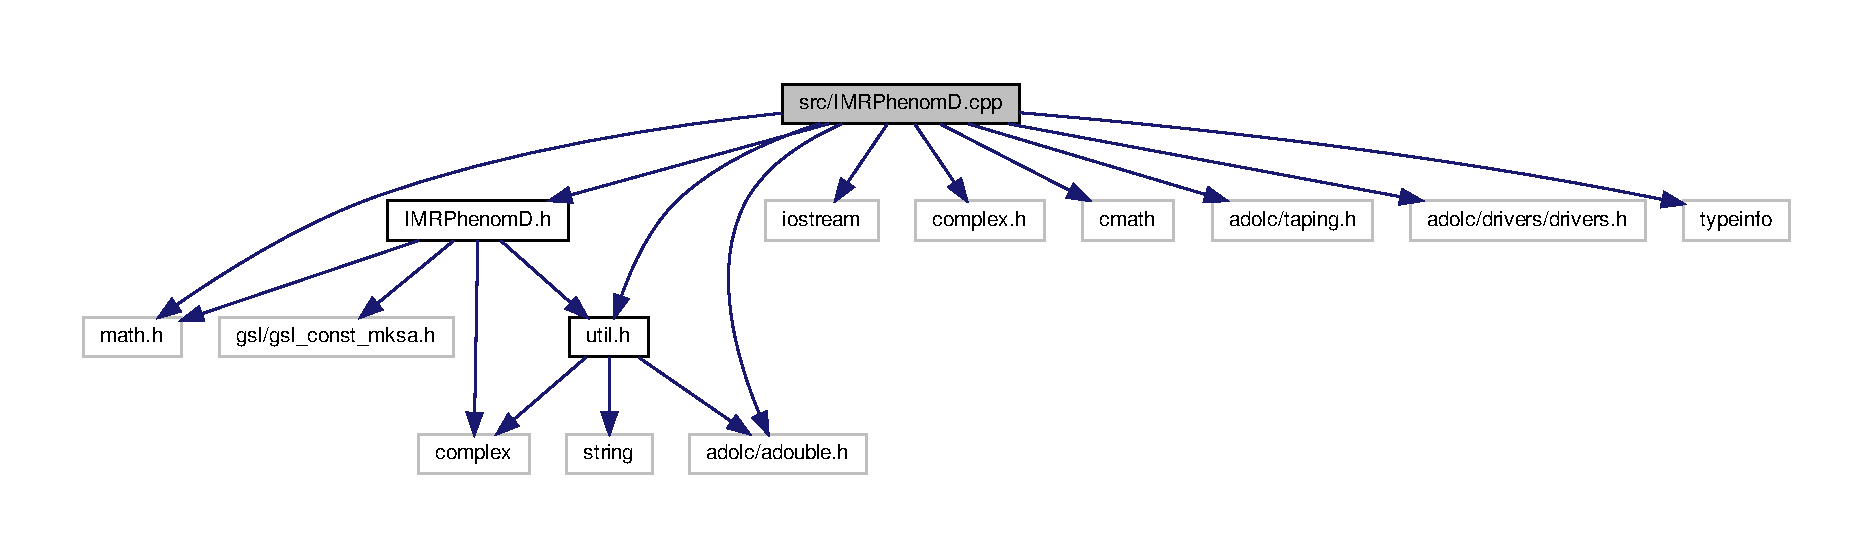
\includegraphics[width=350pt]{IMRPhenomD_8cpp__incl}
\end{center}
\end{figure}
\doxysubsection*{Macros}
\begin{DoxyCompactItemize}
\item 
\mbox{\Hypertarget{IMRPhenomD_8cpp_a71a771d0580911cb2c5fe43e369c744a}\label{IMRPhenomD_8cpp_a71a771d0580911cb2c5fe43e369c744a}} 
\#define {\bfseries omp}~ignore
\end{DoxyCompactItemize}
\doxysubsection*{Variables}
\begin{DoxyCompactItemize}
\item 
\mbox{\Hypertarget{IMRPhenomD_8cpp_a444656d90e803dcd8c71afc8d27898dd}\label{IMRPhenomD_8cpp_a444656d90e803dcd8c71afc8d27898dd}} 
double {\bfseries log\+\_\+64} = 4.\+15888308336
\end{DoxyCompactItemize}


\doxysubsection{Detailed Description}
File that includes all the low level functions that go into constructing the waveform

Matches L\+A\+Lsuite -- 2019\+\_\+09\+\_\+25

Two versions of Q\+NM fitting -- one matches L\+A\+L\+Suites\textquotesingle{} implementation, and is probably more accuate, but involves G\+SL fitting (ie not A\+D\+O\+LC friendly). The other version ensures A\+D\+O\+LC and numerical versions match -- for testing -- just comment out one option if testing (only f\+RD and fdamp) 
\hypertarget{mcmc__routines_8cpp}{}\section{src/mcmc\+\_\+routines.cpp File Reference}
\label{mcmc__routines_8cpp}\index{src/mcmc\+\_\+routines.\+cpp@{src/mcmc\+\_\+routines.\+cpp}}
{\ttfamily \#include \char`\"{}mcmc\+\_\+routines.\+h\char`\"{}}\newline
{\ttfamily \#include \char`\"{}waveform\+\_\+generator.\+h\char`\"{}}\newline
{\ttfamily \#include \char`\"{}util.\+h\char`\"{}}\newline
{\ttfamily \#include \char`\"{}waveform\+\_\+util.\+h\char`\"{}}\newline
{\ttfamily \#include $<$iostream$>$}\newline
{\ttfamily \#include $<$vector$>$}\newline
{\ttfamily \#include $<$complex$>$}\newline
{\ttfamily \#include $<$fftw3.\+h$>$}\newline
{\ttfamily \#include $<$algorithm$>$}\newline
Include dependency graph for mcmc\+\_\+routines.\+cpp\+:\nopagebreak
\begin{figure}[H]
\begin{center}
\leavevmode
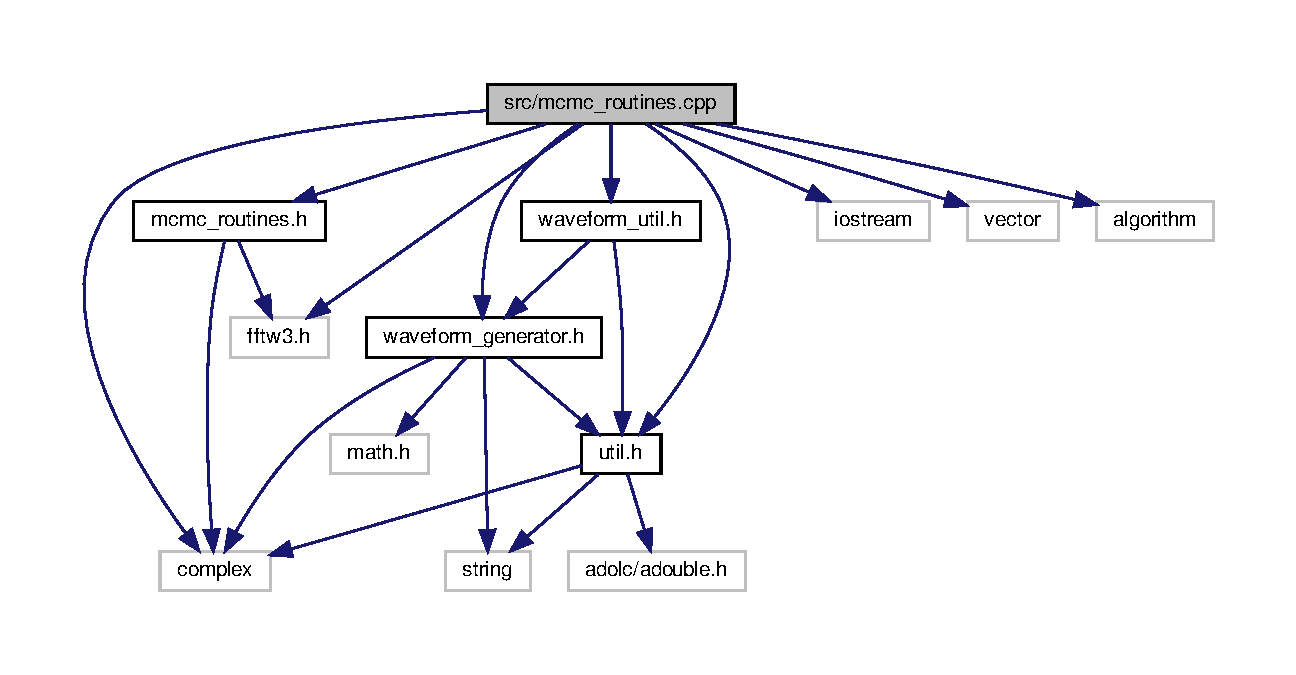
\includegraphics[width=350pt]{mcmc__routines_8cpp__incl}
\end{center}
\end{figure}
\subsection*{Functions}
\begin{DoxyCompactItemize}
\item 
double \hyperlink{mcmc__routines_8cpp_abd627450e43bf7ef683d875d804b7503}{maximized\+\_\+coal\+\_\+log\+\_\+likelihood\+\_\+\+I\+M\+R\+PhenomD} (double $\ast$frequencies, int length, std\+::complex$<$ double $>$ $\ast$data, double $\ast$noise, double S\+NR, double chirpmass, double symmetric\+\_\+mass\+\_\+ratio, double spin1, double spin2, bool N\+Sflag, \hyperlink{structfftw__outline}{fftw\+\_\+outline} $\ast$plan)
\begin{DoxyCompactList}\small\item\em Function to calculate the log Likelihood as defined by -\/1/2 (d-\/h$\vert$d-\/h) maximized over the extrinsic parameters phic and tc. \end{DoxyCompactList}\item 
double \hyperlink{mcmc__routines_8cpp_ae78896f8e8acd8dfaff6ff33a732284a}{maximized\+\_\+coal\+\_\+log\+\_\+likelihood\+\_\+\+I\+M\+R\+PhenomD} (double $\ast$frequencies, size\+\_\+t length, double $\ast$real\+\_\+data, double $\ast$imag\+\_\+data, double $\ast$noise, double S\+NR, double chirpmass, double symmetric\+\_\+mass\+\_\+ratio, double spin1, double spin2, bool N\+Sflag)
\item 
double \hyperlink{mcmc__routines_8cpp_a2635acb06ca0e448854aaab3fd7037c3}{maximized\+\_\+coal\+\_\+log\+\_\+likelihood\+\_\+\+I\+M\+R\+PhenomD} (double $\ast$frequencies, size\+\_\+t length, double $\ast$real\+\_\+data, double $\ast$imag\+\_\+data, double $\ast$noise, double S\+NR, double chirpmass, double symmetric\+\_\+mass\+\_\+ratio, double spin1, double spin2, bool N\+Sflag, \hyperlink{structfftw__outline}{fftw\+\_\+outline} $\ast$plan)
\item 
double \hyperlink{mcmc__routines_8cpp_ac66db6fc5c75ee33b84a48724b4738ef}{maximized\+\_\+coal\+\_\+log\+\_\+likelihood\+\_\+\+I\+M\+R\+Phenom\+D\+\_\+\+Full\+\_\+\+Param} (double $\ast$frequencies, int length, std\+::complex$<$ double $>$ $\ast$data, double $\ast$noise, double chirpmass, double symmetric\+\_\+mass\+\_\+ratio, double spin1, double spin2, double Luminosity\+\_\+\+Distance, double theta, double phi, double iota, bool N\+Sflag, \hyperlink{structfftw__outline}{fftw\+\_\+outline} $\ast$plan)
\item 
double \hyperlink{mcmc__routines_8cpp_a2322ab4b42380145e742ad564c643874}{maximized\+\_\+coal\+\_\+log\+\_\+likelihood\+\_\+\+I\+M\+R\+Phenom\+D\+\_\+\+Full\+\_\+\+Param} (double $\ast$frequencies, size\+\_\+t length, double $\ast$real\+\_\+data, double $\ast$imag\+\_\+data, double $\ast$noise, double chirpmass, double symmetric\+\_\+mass\+\_\+ratio, double spin1, double spin2, double Luminosity\+\_\+\+Distance, double theta, double phi, double iota, bool N\+Sflag)
\item 
double \hyperlink{mcmc__routines_8cpp_a3fbdbcf0651bad5541eb6e366c62de23}{maximized\+\_\+coal\+\_\+log\+\_\+likelihood\+\_\+\+I\+M\+R\+Phenom\+D\+\_\+\+Full\+\_\+\+Param} (double $\ast$frequencies, size\+\_\+t length, double $\ast$real\+\_\+data, double $\ast$imag\+\_\+data, double $\ast$noise, double chirpmass, double symmetric\+\_\+mass\+\_\+ratio, double spin1, double spin2, double Luminosity\+\_\+\+Distance, double theta, double phi, double iota, bool N\+Sflag, \hyperlink{structfftw__outline}{fftw\+\_\+outline} $\ast$plan)
\item 
\mbox{\Hypertarget{mcmc__routines_8cpp_a1599f89f2f16fbd3d5e95f87f48f88a0}\label{mcmc__routines_8cpp_a1599f89f2f16fbd3d5e95f87f48f88a0}} 
void {\bfseries initiate\+\_\+likelihood\+\_\+function} (\hyperlink{structfftw__outline}{fftw\+\_\+outline} $\ast$plan, int length)
\item 
\mbox{\Hypertarget{mcmc__routines_8cpp_a1433ee87cc1dd700874c1db0b1740d7c}\label{mcmc__routines_8cpp_a1433ee87cc1dd700874c1db0b1740d7c}} 
void {\bfseries deactivate\+\_\+likelihood\+\_\+function} (\hyperlink{structfftw__outline}{fftw\+\_\+outline} $\ast$plan)
\end{DoxyCompactItemize}


\subsection{Detailed Description}
Routines for implementation in M\+C\+MC algorithms 

\subsection{Function Documentation}
\mbox{\Hypertarget{mcmc__routines_8cpp_abd627450e43bf7ef683d875d804b7503}\label{mcmc__routines_8cpp_abd627450e43bf7ef683d875d804b7503}} 
\index{mcmc\+\_\+routines.\+cpp@{mcmc\+\_\+routines.\+cpp}!maximized\+\_\+coal\+\_\+log\+\_\+likelihood\+\_\+\+I\+M\+R\+PhenomD@{maximized\+\_\+coal\+\_\+log\+\_\+likelihood\+\_\+\+I\+M\+R\+PhenomD}}
\index{maximized\+\_\+coal\+\_\+log\+\_\+likelihood\+\_\+\+I\+M\+R\+PhenomD@{maximized\+\_\+coal\+\_\+log\+\_\+likelihood\+\_\+\+I\+M\+R\+PhenomD}!mcmc\+\_\+routines.\+cpp@{mcmc\+\_\+routines.\+cpp}}
\subsubsection{\texorpdfstring{maximized\+\_\+coal\+\_\+log\+\_\+likelihood\+\_\+\+I\+M\+R\+Phenom\+D()}{maximized\_coal\_log\_likelihood\_IMRPhenomD()}\hspace{0.1cm}{\footnotesize\ttfamily [1/3]}}
{\footnotesize\ttfamily double maximized\+\_\+coal\+\_\+log\+\_\+likelihood\+\_\+\+I\+M\+R\+PhenomD (\begin{DoxyParamCaption}\item[{double $\ast$}]{frequencies,  }\item[{int}]{length,  }\item[{std\+::complex$<$ double $>$ $\ast$}]{data,  }\item[{double $\ast$}]{noise,  }\item[{double}]{S\+NR,  }\item[{double}]{chirpmass,  }\item[{double}]{symmetric\+\_\+mass\+\_\+ratio,  }\item[{double}]{spin1,  }\item[{double}]{spin2,  }\item[{bool}]{N\+Sflag,  }\item[{\hyperlink{structfftw__outline}{fftw\+\_\+outline} $\ast$}]{plan }\end{DoxyParamCaption})}



Function to calculate the log Likelihood as defined by -\/1/2 (d-\/h$\vert$d-\/h) maximized over the extrinsic parameters phic and tc. 

frequency array must be uniform spacing -\/ this shouldn\textquotesingle{}t be a problem when working with real data as D\+FT return uniform spacing 
\begin{DoxyParams}{Parameters}
{\em chirpmass} & in solar masses \\
\hline
\end{DoxyParams}
\mbox{\Hypertarget{mcmc__routines_8cpp_ae78896f8e8acd8dfaff6ff33a732284a}\label{mcmc__routines_8cpp_ae78896f8e8acd8dfaff6ff33a732284a}} 
\index{mcmc\+\_\+routines.\+cpp@{mcmc\+\_\+routines.\+cpp}!maximized\+\_\+coal\+\_\+log\+\_\+likelihood\+\_\+\+I\+M\+R\+PhenomD@{maximized\+\_\+coal\+\_\+log\+\_\+likelihood\+\_\+\+I\+M\+R\+PhenomD}}
\index{maximized\+\_\+coal\+\_\+log\+\_\+likelihood\+\_\+\+I\+M\+R\+PhenomD@{maximized\+\_\+coal\+\_\+log\+\_\+likelihood\+\_\+\+I\+M\+R\+PhenomD}!mcmc\+\_\+routines.\+cpp@{mcmc\+\_\+routines.\+cpp}}
\subsubsection{\texorpdfstring{maximized\+\_\+coal\+\_\+log\+\_\+likelihood\+\_\+\+I\+M\+R\+Phenom\+D()}{maximized\_coal\_log\_likelihood\_IMRPhenomD()}\hspace{0.1cm}{\footnotesize\ttfamily [2/3]}}
{\footnotesize\ttfamily double maximized\+\_\+coal\+\_\+log\+\_\+likelihood\+\_\+\+I\+M\+R\+PhenomD (\begin{DoxyParamCaption}\item[{double $\ast$}]{frequencies,  }\item[{size\+\_\+t}]{length,  }\item[{double $\ast$}]{real\+\_\+data,  }\item[{double $\ast$}]{imag\+\_\+data,  }\item[{double $\ast$}]{noise,  }\item[{double}]{S\+NR,  }\item[{double}]{chirpmass,  }\item[{double}]{symmetric\+\_\+mass\+\_\+ratio,  }\item[{double}]{spin1,  }\item[{double}]{spin2,  }\item[{bool}]{N\+Sflag }\end{DoxyParamCaption})}


\begin{DoxyParams}{Parameters}
{\em chirpmass} & in solar masses \\
\hline
\end{DoxyParams}
\mbox{\Hypertarget{mcmc__routines_8cpp_a2635acb06ca0e448854aaab3fd7037c3}\label{mcmc__routines_8cpp_a2635acb06ca0e448854aaab3fd7037c3}} 
\index{mcmc\+\_\+routines.\+cpp@{mcmc\+\_\+routines.\+cpp}!maximized\+\_\+coal\+\_\+log\+\_\+likelihood\+\_\+\+I\+M\+R\+PhenomD@{maximized\+\_\+coal\+\_\+log\+\_\+likelihood\+\_\+\+I\+M\+R\+PhenomD}}
\index{maximized\+\_\+coal\+\_\+log\+\_\+likelihood\+\_\+\+I\+M\+R\+PhenomD@{maximized\+\_\+coal\+\_\+log\+\_\+likelihood\+\_\+\+I\+M\+R\+PhenomD}!mcmc\+\_\+routines.\+cpp@{mcmc\+\_\+routines.\+cpp}}
\subsubsection{\texorpdfstring{maximized\+\_\+coal\+\_\+log\+\_\+likelihood\+\_\+\+I\+M\+R\+Phenom\+D()}{maximized\_coal\_log\_likelihood\_IMRPhenomD()}\hspace{0.1cm}{\footnotesize\ttfamily [3/3]}}
{\footnotesize\ttfamily double maximized\+\_\+coal\+\_\+log\+\_\+likelihood\+\_\+\+I\+M\+R\+PhenomD (\begin{DoxyParamCaption}\item[{double $\ast$}]{frequencies,  }\item[{size\+\_\+t}]{length,  }\item[{double $\ast$}]{real\+\_\+data,  }\item[{double $\ast$}]{imag\+\_\+data,  }\item[{double $\ast$}]{noise,  }\item[{double}]{S\+NR,  }\item[{double}]{chirpmass,  }\item[{double}]{symmetric\+\_\+mass\+\_\+ratio,  }\item[{double}]{spin1,  }\item[{double}]{spin2,  }\item[{bool}]{N\+Sflag,  }\item[{\hyperlink{structfftw__outline}{fftw\+\_\+outline} $\ast$}]{plan }\end{DoxyParamCaption})}


\begin{DoxyParams}{Parameters}
{\em chirpmass} & in solar masses \\
\hline
\end{DoxyParams}
\mbox{\Hypertarget{mcmc__routines_8cpp_ac66db6fc5c75ee33b84a48724b4738ef}\label{mcmc__routines_8cpp_ac66db6fc5c75ee33b84a48724b4738ef}} 
\index{mcmc\+\_\+routines.\+cpp@{mcmc\+\_\+routines.\+cpp}!maximized\+\_\+coal\+\_\+log\+\_\+likelihood\+\_\+\+I\+M\+R\+Phenom\+D\+\_\+\+Full\+\_\+\+Param@{maximized\+\_\+coal\+\_\+log\+\_\+likelihood\+\_\+\+I\+M\+R\+Phenom\+D\+\_\+\+Full\+\_\+\+Param}}
\index{maximized\+\_\+coal\+\_\+log\+\_\+likelihood\+\_\+\+I\+M\+R\+Phenom\+D\+\_\+\+Full\+\_\+\+Param@{maximized\+\_\+coal\+\_\+log\+\_\+likelihood\+\_\+\+I\+M\+R\+Phenom\+D\+\_\+\+Full\+\_\+\+Param}!mcmc\+\_\+routines.\+cpp@{mcmc\+\_\+routines.\+cpp}}
\subsubsection{\texorpdfstring{maximized\+\_\+coal\+\_\+log\+\_\+likelihood\+\_\+\+I\+M\+R\+Phenom\+D\+\_\+\+Full\+\_\+\+Param()}{maximized\_coal\_log\_likelihood\_IMRPhenomD\_Full\_Param()}\hspace{0.1cm}{\footnotesize\ttfamily [1/3]}}
{\footnotesize\ttfamily double maximized\+\_\+coal\+\_\+log\+\_\+likelihood\+\_\+\+I\+M\+R\+Phenom\+D\+\_\+\+Full\+\_\+\+Param (\begin{DoxyParamCaption}\item[{double $\ast$}]{frequencies,  }\item[{int}]{length,  }\item[{std\+::complex$<$ double $>$ $\ast$}]{data,  }\item[{double $\ast$}]{noise,  }\item[{double}]{chirpmass,  }\item[{double}]{symmetric\+\_\+mass\+\_\+ratio,  }\item[{double}]{spin1,  }\item[{double}]{spin2,  }\item[{double}]{Luminosity\+\_\+\+Distance,  }\item[{double}]{theta,  }\item[{double}]{phi,  }\item[{double}]{iota,  }\item[{bool}]{N\+Sflag,  }\item[{\hyperlink{structfftw__outline}{fftw\+\_\+outline} $\ast$}]{plan }\end{DoxyParamCaption})}


\begin{DoxyParams}{Parameters}
{\em chirpmass} & in solar masses \\
\hline
\end{DoxyParams}
\mbox{\Hypertarget{mcmc__routines_8cpp_a2322ab4b42380145e742ad564c643874}\label{mcmc__routines_8cpp_a2322ab4b42380145e742ad564c643874}} 
\index{mcmc\+\_\+routines.\+cpp@{mcmc\+\_\+routines.\+cpp}!maximized\+\_\+coal\+\_\+log\+\_\+likelihood\+\_\+\+I\+M\+R\+Phenom\+D\+\_\+\+Full\+\_\+\+Param@{maximized\+\_\+coal\+\_\+log\+\_\+likelihood\+\_\+\+I\+M\+R\+Phenom\+D\+\_\+\+Full\+\_\+\+Param}}
\index{maximized\+\_\+coal\+\_\+log\+\_\+likelihood\+\_\+\+I\+M\+R\+Phenom\+D\+\_\+\+Full\+\_\+\+Param@{maximized\+\_\+coal\+\_\+log\+\_\+likelihood\+\_\+\+I\+M\+R\+Phenom\+D\+\_\+\+Full\+\_\+\+Param}!mcmc\+\_\+routines.\+cpp@{mcmc\+\_\+routines.\+cpp}}
\subsubsection{\texorpdfstring{maximized\+\_\+coal\+\_\+log\+\_\+likelihood\+\_\+\+I\+M\+R\+Phenom\+D\+\_\+\+Full\+\_\+\+Param()}{maximized\_coal\_log\_likelihood\_IMRPhenomD\_Full\_Param()}\hspace{0.1cm}{\footnotesize\ttfamily [2/3]}}
{\footnotesize\ttfamily double maximized\+\_\+coal\+\_\+log\+\_\+likelihood\+\_\+\+I\+M\+R\+Phenom\+D\+\_\+\+Full\+\_\+\+Param (\begin{DoxyParamCaption}\item[{double $\ast$}]{frequencies,  }\item[{size\+\_\+t}]{length,  }\item[{double $\ast$}]{real\+\_\+data,  }\item[{double $\ast$}]{imag\+\_\+data,  }\item[{double $\ast$}]{noise,  }\item[{double}]{chirpmass,  }\item[{double}]{symmetric\+\_\+mass\+\_\+ratio,  }\item[{double}]{spin1,  }\item[{double}]{spin2,  }\item[{double}]{Luminosity\+\_\+\+Distance,  }\item[{double}]{theta,  }\item[{double}]{phi,  }\item[{double}]{iota,  }\item[{bool}]{N\+Sflag }\end{DoxyParamCaption})}


\begin{DoxyParams}{Parameters}
{\em chirpmass} & in solar masses \\
\hline
\end{DoxyParams}
\mbox{\Hypertarget{mcmc__routines_8cpp_a3fbdbcf0651bad5541eb6e366c62de23}\label{mcmc__routines_8cpp_a3fbdbcf0651bad5541eb6e366c62de23}} 
\index{mcmc\+\_\+routines.\+cpp@{mcmc\+\_\+routines.\+cpp}!maximized\+\_\+coal\+\_\+log\+\_\+likelihood\+\_\+\+I\+M\+R\+Phenom\+D\+\_\+\+Full\+\_\+\+Param@{maximized\+\_\+coal\+\_\+log\+\_\+likelihood\+\_\+\+I\+M\+R\+Phenom\+D\+\_\+\+Full\+\_\+\+Param}}
\index{maximized\+\_\+coal\+\_\+log\+\_\+likelihood\+\_\+\+I\+M\+R\+Phenom\+D\+\_\+\+Full\+\_\+\+Param@{maximized\+\_\+coal\+\_\+log\+\_\+likelihood\+\_\+\+I\+M\+R\+Phenom\+D\+\_\+\+Full\+\_\+\+Param}!mcmc\+\_\+routines.\+cpp@{mcmc\+\_\+routines.\+cpp}}
\subsubsection{\texorpdfstring{maximized\+\_\+coal\+\_\+log\+\_\+likelihood\+\_\+\+I\+M\+R\+Phenom\+D\+\_\+\+Full\+\_\+\+Param()}{maximized\_coal\_log\_likelihood\_IMRPhenomD\_Full\_Param()}\hspace{0.1cm}{\footnotesize\ttfamily [3/3]}}
{\footnotesize\ttfamily double maximized\+\_\+coal\+\_\+log\+\_\+likelihood\+\_\+\+I\+M\+R\+Phenom\+D\+\_\+\+Full\+\_\+\+Param (\begin{DoxyParamCaption}\item[{double $\ast$}]{frequencies,  }\item[{size\+\_\+t}]{length,  }\item[{double $\ast$}]{real\+\_\+data,  }\item[{double $\ast$}]{imag\+\_\+data,  }\item[{double $\ast$}]{noise,  }\item[{double}]{chirpmass,  }\item[{double}]{symmetric\+\_\+mass\+\_\+ratio,  }\item[{double}]{spin1,  }\item[{double}]{spin2,  }\item[{double}]{Luminosity\+\_\+\+Distance,  }\item[{double}]{theta,  }\item[{double}]{phi,  }\item[{double}]{iota,  }\item[{bool}]{N\+Sflag,  }\item[{\hyperlink{structfftw__outline}{fftw\+\_\+outline} $\ast$}]{plan }\end{DoxyParamCaption})}


\begin{DoxyParams}{Parameters}
{\em chirpmass} & in solar masses \\
\hline
\end{DoxyParams}

\hypertarget{noise__util_8cpp}{}\section{src/noise\+\_\+util.cpp File Reference}
\label{noise__util_8cpp}\index{src/noise\+\_\+util.\+cpp@{src/noise\+\_\+util.\+cpp}}
{\ttfamily \#include \char`\"{}noise\+\_\+util.\+h\char`\"{}}\newline
{\ttfamily \#include $<$fstream$>$}\newline
{\ttfamily \#include $<$iostream$>$}\newline
{\ttfamily \#include $<$string$>$}\newline
{\ttfamily \#include $<$math.\+h$>$}\newline
Include dependency graph for noise\+\_\+util.\+cpp\+:\nopagebreak
\begin{figure}[H]
\begin{center}
\leavevmode
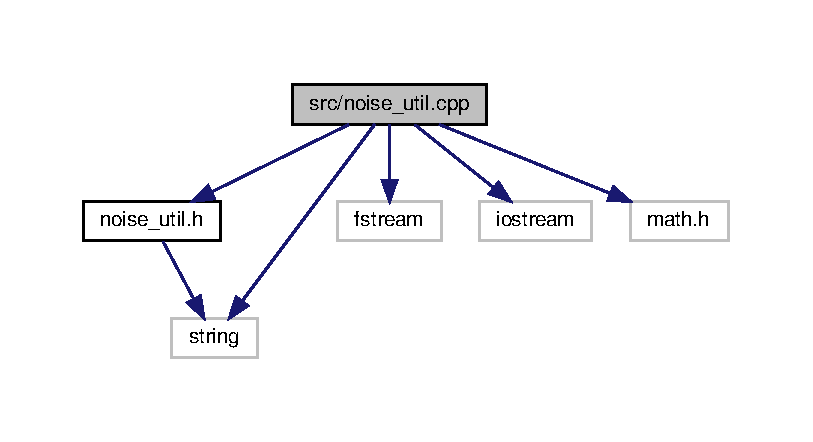
\includegraphics[width=350pt]{noise__util_8cpp__incl}
\end{center}
\end{figure}
\subsection*{Functions}
\begin{DoxyCompactItemize}
\item 
void \hyperlink{noise__util_8cpp_ac7de9bc27fe8b7bc13e4c0a356d3b18d}{populate\+\_\+noise} (double $\ast$frequencies, std\+::string detector, double $\ast$noise\+\_\+root, int length)
\begin{DoxyCompactList}\small\item\em Function to populate the squareroot of the noise curve for various detectors. \end{DoxyCompactList}\item 
\mbox{\Hypertarget{noise__util_8cpp_a6e657285283899f91aa3b7ec7963c120}\label{noise__util_8cpp_a6e657285283899f91aa3b7ec7963c120}} 
double {\bfseries a\+L\+I\+G\+O\+\_\+analytic} (double f)
\item 
\mbox{\Hypertarget{noise__util_8cpp_a2e29bfa3018d037af4d1b52cabe47d39}\label{noise__util_8cpp_a2e29bfa3018d037af4d1b52cabe47d39}} 
double {\bfseries Hanford\+\_\+\+O1\+\_\+fitted} (double f)
\end{DoxyCompactItemize}


\subsection{Detailed Description}
Routines to construct noise curves for various detectors 

\subsection{Function Documentation}
\mbox{\Hypertarget{noise__util_8cpp_ac7de9bc27fe8b7bc13e4c0a356d3b18d}\label{noise__util_8cpp_ac7de9bc27fe8b7bc13e4c0a356d3b18d}} 
\index{noise\+\_\+util.\+cpp@{noise\+\_\+util.\+cpp}!populate\+\_\+noise@{populate\+\_\+noise}}
\index{populate\+\_\+noise@{populate\+\_\+noise}!noise\+\_\+util.\+cpp@{noise\+\_\+util.\+cpp}}
\subsubsection{\texorpdfstring{populate\+\_\+noise()}{populate\_noise()}}
{\footnotesize\ttfamily void populate\+\_\+noise (\begin{DoxyParamCaption}\item[{double $\ast$}]{frequencies,  }\item[{std\+::string}]{detector,  }\item[{double $\ast$}]{noise\+\_\+root,  }\item[{int}]{length }\end{DoxyParamCaption})}



Function to populate the squareroot of the noise curve for various detectors. 

If frequencies are left as N\+U\+LL, standard frequency spacing is applied and the frequencies are returned, in which case the frequencies argument becomes an output array

Detector names must be spelled exactly

Detectors include\+: a\+L\+I\+G\+O\+\_\+analytic, Hanford\+\_\+\+O1\+\_\+fitted 
\begin{DoxyParams}{Parameters}
{\em frequencies} & double array of frquencies (N\+U\+LL) \\
\hline
{\em detector} & String to designate the detector noise curve to be used \\
\hline
{\em noise\+\_\+root} & ouptput double array for the square root of the P\+SD of the noise of the specified detector \\
\hline
{\em length} & integer length of the output and input arrays \\
\hline
\end{DoxyParams}

\hypertarget{ppE__IMRPhenomD_8cpp}{}\section{src/pp\+E\+\_\+\+I\+M\+R\+PhenomD.cpp File Reference}
\label{ppE__IMRPhenomD_8cpp}\index{src/pp\+E\+\_\+\+I\+M\+R\+Phenom\+D.\+cpp@{src/pp\+E\+\_\+\+I\+M\+R\+Phenom\+D.\+cpp}}
{\ttfamily \#include \char`\"{}pp\+E\+\_\+\+I\+M\+R\+Phenom\+D.\+h\char`\"{}}\newline
{\ttfamily \#include $<$math.\+h$>$}\newline
{\ttfamily \#include $<$adolc/adouble.\+h$>$}\newline
{\ttfamily \#include $<$adolc/taping.\+h$>$}\newline
{\ttfamily \#include $<$adolc/drivers/drivers.\+h$>$}\newline
{\ttfamily \#include $<$iostream$>$}\newline
{\ttfamily \#include $<$cmath$>$}\newline
{\ttfamily \#include $<$complex$>$}\newline
{\ttfamily \#include \char`\"{}util.\+h\char`\"{}}\newline
Include dependency graph for pp\+E\+\_\+\+I\+M\+R\+Phenom\+D.\+cpp\+:\nopagebreak
\begin{figure}[H]
\begin{center}
\leavevmode
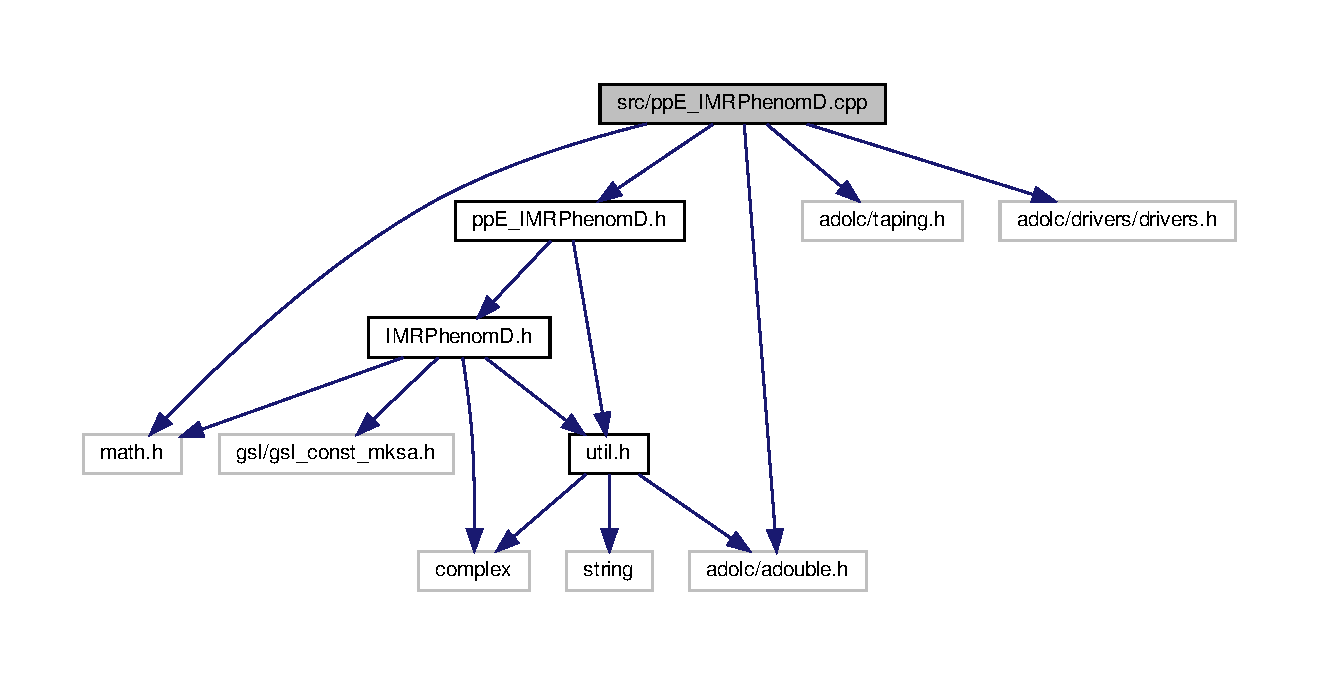
\includegraphics[width=350pt]{ppE__IMRPhenomD_8cpp__incl}
\end{center}
\end{figure}


\subsection{Detailed Description}
File for the implementation of the ppE formalism for testing GR

Extends the \hyperlink{classIMRPhenomD}{I\+M\+R\+PhenomD} template to include non-\/\+GR phase terms

Supported waveforms\+: ppE Inspiral, ppE I\+MR, d\+CS, Ed\+GB 
\hypertarget{util_8cpp}{}\doxysection{src/util.cpp File Reference}
\label{util_8cpp}\index{src/util.cpp@{src/util.cpp}}
{\ttfamily \#include \char`\"{}util.\+h\char`\"{}}\newline
{\ttfamily \#include \char`\"{}G\+W\+A\+T\+Config.\+h\char`\"{}}\newline
{\ttfamily \#include \char`\"{}D\+\_\+\+Z\+\_\+\+Config.\+h\char`\"{}}\newline
{\ttfamily \#include $<$math.\+h$>$}\newline
{\ttfamily \#include $<$string$>$}\newline
{\ttfamily \#include $<$string.\+h$>$}\newline
{\ttfamily \#include $<$complex$>$}\newline
{\ttfamily \#include $<$iostream$>$}\newline
{\ttfamily \#include $<$stdio.\+h$>$}\newline
{\ttfamily \#include $<$fstream$>$}\newline
{\ttfamily \#include $<$adolc/adouble.\+h$>$}\newline
{\ttfamily \#include $<$gsl/gsl\+\_\+interp.\+h$>$}\newline
{\ttfamily \#include $<$gsl/gsl\+\_\+spline.\+h$>$}\newline
{\ttfamily \#include $<$gsl/gsl\+\_\+errno.\+h$>$}\newline
{\ttfamily \#include $<$gsl/gsl\+\_\+matrix\+\_\+double.\+h$>$}\newline
{\ttfamily \#include $<$gsl/gsl\+\_\+linalg.\+h$>$}\newline
{\ttfamily \#include $<$gsl/gsl\+\_\+rng.\+h$>$}\newline
{\ttfamily \#include $<$gsl/gsl\+\_\+randist.\+h$>$}\newline
Include dependency graph for util.\+cpp\+:
\nopagebreak
\begin{figure}[H]
\begin{center}
\leavevmode
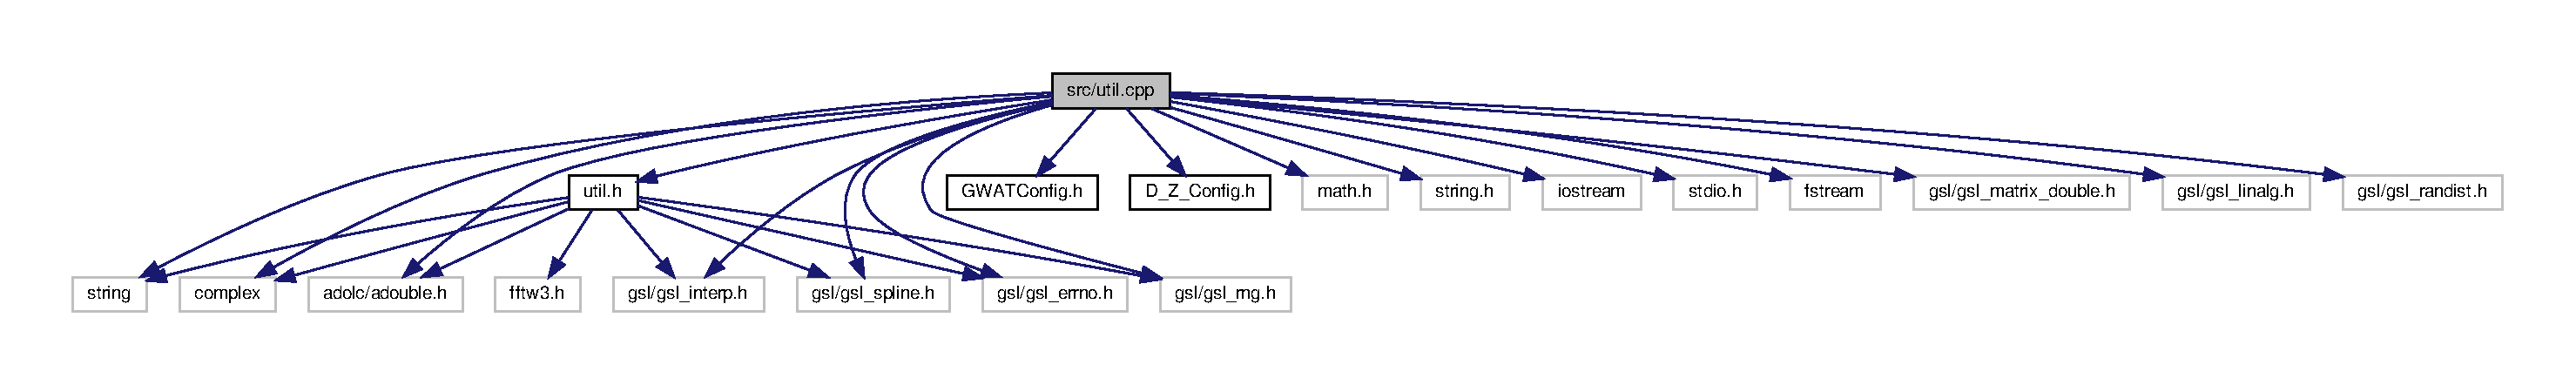
\includegraphics[width=350pt]{util_8cpp__incl}
\end{center}
\end{figure}
\doxysubsection*{Functions}
\begin{DoxyCompactItemize}
\item 
void \mbox{\hyperlink{util_8cpp_abd99f3492eda3805283a6a6c1161f61f}{initiate\+\_\+\+Lum\+D\+\_\+\+Z\+\_\+interp}} (gsl\+\_\+interp\+\_\+accel $\ast$$\ast$Z\+\_\+\+D\+L\+\_\+accel\+\_\+ptr, gsl\+\_\+spline $\ast$$\ast$Z\+\_\+\+D\+L\+\_\+spline\+\_\+ptr)
\begin{DoxyCompactList}\small\item\em Function that uses the G\+SL libraries to interpolate pre-\/calculated Z-\/\+D\+\_\+L data. \end{DoxyCompactList}\item 
\mbox{\Hypertarget{util_8cpp_a9ec71fbb0a133a3099b570e6cfe4c116}\label{util_8cpp_a9ec71fbb0a133a3099b570e6cfe4c116}} 
void \mbox{\hyperlink{util_8cpp_a9ec71fbb0a133a3099b570e6cfe4c116}{free\+\_\+\+Lum\+D\+\_\+\+Z\+\_\+interp}} (gsl\+\_\+interp\+\_\+accel $\ast$$\ast$Z\+\_\+\+D\+L\+\_\+accel\+\_\+ptr, gsl\+\_\+spline $\ast$$\ast$Z\+\_\+\+D\+L\+\_\+spline\+\_\+ptr)
\begin{DoxyCompactList}\small\item\em Frees the allocated interpolation function. \end{DoxyCompactList}\item 
adouble \mbox{\hyperlink{util_8cpp_aec48ba6d02ebe433a684e09884e6a31b}{Z\+\_\+from\+\_\+\+D\+L\+\_\+interp}} (adouble DL, gsl\+\_\+interp\+\_\+accel $\ast$Z\+\_\+\+D\+L\+\_\+accel\+\_\+ptr, gsl\+\_\+spline $\ast$Z\+\_\+\+D\+L\+\_\+spline\+\_\+ptr)
\item 
double \mbox{\hyperlink{util_8cpp_a8d080a588955cc9cb0a4efc831187936}{Z\+\_\+from\+\_\+\+D\+L\+\_\+interp}} (double DL, gsl\+\_\+interp\+\_\+accel $\ast$Z\+\_\+\+D\+L\+\_\+accel\+\_\+ptr, gsl\+\_\+spline $\ast$Z\+\_\+\+D\+L\+\_\+spline\+\_\+ptr)
\item 
double \mbox{\hyperlink{util_8cpp_a415ef00e103efe73c8eabc235b202b12}{Z\+\_\+from\+\_\+\+DL}} (double DL, std\+::string cosmology)
\begin{DoxyCompactList}\small\item\em Calculates the redshift given the luminosity distance. \end{DoxyCompactList}\item 
\mbox{\Hypertarget{util_8cpp_a15f9dbddbe35da0c1b39ea0f7ce6870e}\label{util_8cpp_a15f9dbddbe35da0c1b39ea0f7ce6870e}} 
adouble \mbox{\hyperlink{util_8cpp_a15f9dbddbe35da0c1b39ea0f7ce6870e}{Z\+\_\+from\+\_\+\+DL}} (adouble DL, std\+::string cosmology)
\begin{DoxyCompactList}\small\item\em Calculates the redshift given the luminosity distance adouble version for A\+D\+O\+L-\/C implementation. \end{DoxyCompactList}\item 
double \mbox{\hyperlink{util_8cpp_a88960e6947432b203d2c7ebb436e1984}{D\+L\+\_\+from\+\_\+Z}} (double Z, std\+::string cosmology)
\begin{DoxyCompactList}\small\item\em Calculates the luminosity distance given the redshift. \end{DoxyCompactList}\item 
\mbox{\Hypertarget{util_8cpp_ac5495a177f2316ca6dc0904f3643b7f1}\label{util_8cpp_ac5495a177f2316ca6dc0904f3643b7f1}} 
adouble \mbox{\hyperlink{util_8cpp_ac5495a177f2316ca6dc0904f3643b7f1}{D\+L\+\_\+from\+\_\+Z}} (adouble Z, std\+::string cosmology)
\begin{DoxyCompactList}\small\item\em Calculates the luminosity distance given the redshift adouble version for A\+D\+O\+L-\/C implementation. \end{DoxyCompactList}\item 
double \mbox{\hyperlink{util_8cpp_afc70040a4b2855ffc42c1f8b91e87fc2}{cosmology\+\_\+interpolation\+\_\+function}} (double x, double $\ast$coeffs, int interp\+\_\+degree)
\begin{DoxyCompactList}\small\item\em Custom interpolation function used in the cosmology calculations. \end{DoxyCompactList}\item 
\mbox{\Hypertarget{util_8cpp_a89c3042d0c813fd58dcb6a433d26eaa4}\label{util_8cpp_a89c3042d0c813fd58dcb6a433d26eaa4}} 
adouble \mbox{\hyperlink{util_8cpp_a89c3042d0c813fd58dcb6a433d26eaa4}{cosmology\+\_\+interpolation\+\_\+function}} (adouble x, double $\ast$coeffs, int interp\+\_\+degree)
\begin{DoxyCompactList}\small\item\em Custom interpolation function used in the cosmology calculations adouble version for A\+D\+O\+L-\/C. \end{DoxyCompactList}\item 
\mbox{\Hypertarget{util_8cpp_afda1342d7215e52bcbb8f483ca576524}\label{util_8cpp_afda1342d7215e52bcbb8f483ca576524}} 
double \mbox{\hyperlink{util_8cpp_afda1342d7215e52bcbb8f483ca576524}{cosmology\+\_\+lookup}} (std\+::string cosmology)
\begin{DoxyCompactList}\small\item\em Helper function for mapping cosmology name to an internal index. \end{DoxyCompactList}\item 
double \mbox{\hyperlink{util_8cpp_aa82ab145d4f623214c1492589e4327bf}{gsl\+\_\+maxwell\+\_\+boltzmann\+\_\+distribution}} (double sigma, gsl\+\_\+rng $\ast$r)
\begin{DoxyCompactList}\small\item\em Calculates a random number from the Maxwell-\/\+Boltzmann distribution using 3 gaussian random numbers. \end{DoxyCompactList}\item 
\mbox{\Hypertarget{util_8cpp_a588d05c5e239cff9b87a31d20bb6aa78}\label{util_8cpp_a588d05c5e239cff9b87a31d20bb6aa78}} 
{\footnotesize template$<$class T $>$ }\\T {\bfseries copysign\+\_\+internal} (T val, T sign)
\item 
\mbox{\Hypertarget{util_8cpp_a4e97ada4e992cd5ba6ff9eec3e60deed}\label{util_8cpp_a4e97ada4e992cd5ba6ff9eec3e60deed}} 
template double {\bfseries copysign\+\_\+internal$<$ double $>$} (double, double)
\item 
\mbox{\Hypertarget{util_8cpp_a14378a26cefa05a8e718ee0c11b35189}\label{util_8cpp_a14378a26cefa05a8e718ee0c11b35189}} 
template adouble {\bfseries copysign\+\_\+internal$<$ adouble $>$} (adouble, adouble)
\item 
void \mbox{\hyperlink{util_8cpp_aa3b3e1ddc0801e2dcfa09d5683936817}{rm\+\_\+fisher\+\_\+dim}} (double $\ast$$\ast$input, int full\+\_\+dim, double $\ast$$\ast$output, int reduced\+\_\+dim, int $\ast$removed\+\_\+dims)
\begin{DoxyCompactList}\small\item\em Removes a dimension from a matrix (made with fishers in mind, but this is general) \end{DoxyCompactList}\item 
{\footnotesize template$<$class T $>$ }\\void \mbox{\hyperlink{util_8cpp_a9d0768e0355feef9d4d9681e6eed27b4}{list\+\_\+intersect\+\_\+ptrs}} (T $\ast$$\ast$A, int lenA, T $\ast$$\ast$B, int lenB, T $\ast$$\ast$C, int $\ast$lenC)
\begin{DoxyCompactList}\small\item\em Custom list-\/interesction implementation for sorted lists. \end{DoxyCompactList}\item 
\mbox{\Hypertarget{util_8cpp_a27374164e2005c1ca170f7586817e66a}\label{util_8cpp_a27374164e2005c1ca170f7586817e66a}} 
template void {\bfseries list\+\_\+intersect\+\_\+ptrs$<$ double $>$} (double $\ast$$\ast$, int, double $\ast$$\ast$, int, double $\ast$$\ast$, int $\ast$)
\item 
\mbox{\Hypertarget{util_8cpp_a60d139eb80a03e095f710aa1c887af39}\label{util_8cpp_a60d139eb80a03e095f710aa1c887af39}} 
template void {\bfseries list\+\_\+intersect\+\_\+ptrs$<$ adouble $>$} (adouble $\ast$$\ast$, int, adouble $\ast$$\ast$, int, adouble $\ast$$\ast$, int $\ast$)
\item 
\mbox{\Hypertarget{util_8cpp_a456f6392ae12f52dcf78b4fea952940a}\label{util_8cpp_a456f6392ae12f52dcf78b4fea952940a}} 
template void {\bfseries list\+\_\+intersect\+\_\+ptrs$<$ int $>$} (int $\ast$$\ast$, int, int $\ast$$\ast$, int, int $\ast$$\ast$, int $\ast$)
\item 
{\footnotesize template$<$class T $>$ }\\void \mbox{\hyperlink{util_8cpp_a6a20a9cb79b3c847fc75f3e3eb45f933}{list\+\_\+intersect}} (T $\ast$A, int lenA, T $\ast$B, int lenB, T $\ast$$\ast$C, int $\ast$lenC)
\begin{DoxyCompactList}\small\item\em Custom list-\/interesction implementation for sorted lists. \end{DoxyCompactList}\item 
\mbox{\Hypertarget{util_8cpp_a599977e7f7dc2531edd0c6685926e4b8}\label{util_8cpp_a599977e7f7dc2531edd0c6685926e4b8}} 
template void {\bfseries list\+\_\+intersect$<$ double $>$} (double $\ast$, int, double $\ast$, int, double $\ast$$\ast$, int $\ast$)
\item 
\mbox{\Hypertarget{util_8cpp_acf288d7230f786abf3b98eab3bf1b451}\label{util_8cpp_acf288d7230f786abf3b98eab3bf1b451}} 
template void {\bfseries list\+\_\+intersect$<$ adouble $>$} (adouble $\ast$, int, adouble $\ast$, int, adouble $\ast$$\ast$, int $\ast$)
\item 
\mbox{\Hypertarget{util_8cpp_a79c2688dc6d09b4aee47618cd5340819}\label{util_8cpp_a79c2688dc6d09b4aee47618cd5340819}} 
template void {\bfseries list\+\_\+intersect$<$ int $>$} (int $\ast$, int, int $\ast$, int, int $\ast$$\ast$, int $\ast$)
\item 
{\footnotesize template$<$class T $>$ }\\bool \mbox{\hyperlink{util_8cpp_a9631c2bd8b5493af4df2528a44886fc6}{check\+\_\+list}} (T j, T $\ast$list, int length)
\begin{DoxyCompactList}\small\item\em Just a quick utility to see if an item is in a list. \end{DoxyCompactList}\item 
\mbox{\Hypertarget{util_8cpp_a7a29532c684375047abca8ad29d2290c}\label{util_8cpp_a7a29532c684375047abca8ad29d2290c}} 
template bool {\bfseries check\+\_\+list$<$ int $>$} (int, int $\ast$, int)
\item 
\mbox{\Hypertarget{util_8cpp_abcd981405b40454bda795d30ce1fc180}\label{util_8cpp_abcd981405b40454bda795d30ce1fc180}} 
template bool {\bfseries check\+\_\+list$<$ double $>$} (double, double $\ast$, int)
\item 
{\footnotesize template$<$class T $>$ }\\int \mbox{\hyperlink{util_8cpp_af81850392cb5ff136ea8d334952844e0}{check\+\_\+list\+\_\+id}} (T j, T $\ast$list, int length)
\begin{DoxyCompactList}\small\item\em Just a quick utility to see if an item is in a list. \end{DoxyCompactList}\item 
\mbox{\Hypertarget{util_8cpp_a81db2a61b2881d4fe2b7fd12800e077e}\label{util_8cpp_a81db2a61b2881d4fe2b7fd12800e077e}} 
template int {\bfseries check\+\_\+list\+\_\+id$<$ int $>$} (int, int $\ast$, int)
\item 
\mbox{\Hypertarget{util_8cpp_a66acb2ab31057167bc82b7031e7a7b0b}\label{util_8cpp_a66acb2ab31057167bc82b7031e7a7b0b}} 
template int {\bfseries check\+\_\+list\+\_\+id$<$ double $>$} (double, double $\ast$, int)
\item 
\mbox{\Hypertarget{util_8cpp_a11145d2a037fa94ed58393c6f9b7eb6d}\label{util_8cpp_a11145d2a037fa94ed58393c6f9b7eb6d}} 
{\footnotesize template$<$class T $>$ }\\void {\bfseries gsl\+\_\+\+L\+U\+\_\+matrix\+\_\+invert} (T $\ast$$\ast$input, T $\ast$$\ast$inverse, int dim)
\item 
\mbox{\Hypertarget{util_8cpp_aea0c76d4acae4a1c3064a7310b63c0a8}\label{util_8cpp_aea0c76d4acae4a1c3064a7310b63c0a8}} 
template void {\bfseries gsl\+\_\+\+L\+U\+\_\+matrix\+\_\+invert$<$ double $>$} (double $\ast$$\ast$, double $\ast$$\ast$, int)
\item 
\mbox{\Hypertarget{util_8cpp_aba892910f0cef251be3ba7c561290761}\label{util_8cpp_aba892910f0cef251be3ba7c561290761}} 
int {\bfseries gsl\+\_\+cholesky\+\_\+matrix\+\_\+invert} (double $\ast$$\ast$input, double $\ast$$\ast$inverse, int dim)
\item 
int \mbox{\hyperlink{util_8cpp_a8289e1ab34de59220846f1114dd9f667}{normalized\+\_\+gsl\+\_\+cholesky\+\_\+matrix\+\_\+invert}} (double $\ast$$\ast$input, double $\ast$$\ast$inverse, int dim)
\begin{DoxyCompactList}\small\item\em Normalize the Fisher matrix before inversion to try and tame singularity issues\+: \end{DoxyCompactList}\item 
double \mbox{\hyperlink{util_8cpp_a132fb8304c25ab9a2e18327cfc65b013}{std\+\_\+omega}} (double RA, double std\+\_\+\+RA, double std\+\_\+\+D\+EC, double cov\+\_\+\+R\+A\+\_\+\+D\+EC)
\begin{DoxyCompactList}\small\item\em map the error on RA and D\+EC to error on solid angle \textbackslash{}\+Omega \end{DoxyCompactList}\item 
void \mbox{\hyperlink{util_8cpp_a9d3b483a858efb84ce776bed255b6dd6}{print\+Progress}} (double percentage)
\begin{DoxyCompactList}\small\item\em routine to print the progress of a process to the terminal as a progress bar \end{DoxyCompactList}\item 
\mbox{\Hypertarget{util_8cpp_a9d87eefd2881f9d512458bdcb05c9480}\label{util_8cpp_a9d87eefd2881f9d512458bdcb05c9480}} 
void \mbox{\hyperlink{util_8cpp_a9d87eefd2881f9d512458bdcb05c9480}{allocate\+\_\+\+F\+F\+T\+W\+\_\+mem\+\_\+forward}} (\mbox{\hyperlink{structfftw__outline}{fftw\+\_\+outline}} $\ast$plan, int length)
\begin{DoxyCompactList}\small\item\em Allocate memory for F\+F\+T\+W3 methods used in a lot of inner products input is a locally defined structure that houses all the pertinent data. \end{DoxyCompactList}\item 
\mbox{\Hypertarget{util_8cpp_abfb132a88c05af083194d8ee163c6dcd}\label{util_8cpp_abfb132a88c05af083194d8ee163c6dcd}} 
void \mbox{\hyperlink{util_8cpp_abfb132a88c05af083194d8ee163c6dcd}{allocate\+\_\+\+F\+F\+T\+W\+\_\+mem\+\_\+reverse}} (\mbox{\hyperlink{structfftw__outline}{fftw\+\_\+outline}} $\ast$plan, int length)
\begin{DoxyCompactList}\small\item\em Allocate memory for F\+F\+T\+W3 methods used in a lot of inner products --I\+N\+V\+E\+R\+SE input is a locally defined structure that houses all the pertinent data. \end{DoxyCompactList}\item 
\mbox{\Hypertarget{util_8cpp_a564ceafac6d45bfc46b9960ff363be94}\label{util_8cpp_a564ceafac6d45bfc46b9960ff363be94}} 
void \mbox{\hyperlink{util_8cpp_a564ceafac6d45bfc46b9960ff363be94}{deallocate\+\_\+\+F\+F\+T\+W\+\_\+mem}} (\mbox{\hyperlink{structfftw__outline}{fftw\+\_\+outline}} $\ast$plan)
\begin{DoxyCompactList}\small\item\em deallocates the memory used for F\+F\+TW routines \end{DoxyCompactList}\item 
{\footnotesize template$<$class T , class U $>$ }\\void \mbox{\hyperlink{util_8cpp_a168fd7e5d1d20a344c7bc5e6ced76763}{transform\+\_\+parameters}} (\mbox{\hyperlink{classgen__params__base}{gen\+\_\+params\+\_\+base}}$<$ T $>$ $\ast$param\+\_\+in, \mbox{\hyperlink{classgen__params__base}{gen\+\_\+params\+\_\+base}}$<$ U $>$ $\ast$param\+\_\+out)
\begin{DoxyCompactList}\small\item\em Simple utility to copy the members of param\+\_\+in to param\+\_\+out, for whatever types those are. \end{DoxyCompactList}\item 
\mbox{\Hypertarget{util_8cpp_a44e97e344b2c1bce3ec660f34eef801d}\label{util_8cpp_a44e97e344b2c1bce3ec660f34eef801d}} 
bool {\bfseries check\+\_\+mod} (std\+::string generation\+\_\+method)
\item 
\mbox{\Hypertarget{util_8cpp_ac198de6bb481026200d3e7905c6c9e94}\label{util_8cpp_ac198de6bb481026200d3e7905c6c9e94}} 
template void {\bfseries transform\+\_\+parameters$<$ double, adouble $>$} (\mbox{\hyperlink{classgen__params__base}{gen\+\_\+params\+\_\+base}}$<$ double $>$ $\ast$, \mbox{\hyperlink{classgen__params__base}{gen\+\_\+params\+\_\+base}}$<$ adouble $>$ $\ast$)
\item 
{\footnotesize template$<$class T $>$ }\\T \mbox{\hyperlink{util_8cpp_a178bf529eadac2d4e27e6919f322734a}{A0\+\_\+from\+\_\+\+DL}} (T chirpmass, T DL, bool sky\+\_\+average)
\begin{DoxyCompactList}\small\item\em Transforms between chirpmass and DL to overall amplitude factor A0. \end{DoxyCompactList}\item 
\mbox{\Hypertarget{util_8cpp_aa5fc941f2fac67667eabac3b18a0fc1d}\label{util_8cpp_aa5fc941f2fac67667eabac3b18a0fc1d}} 
template double {\bfseries A0\+\_\+from\+\_\+\+D\+L$<$ double $>$} (double, double, bool)
\item 
\mbox{\Hypertarget{util_8cpp_ad2aeb1394d2a4ed95a67b25c45675412}\label{util_8cpp_ad2aeb1394d2a4ed95a67b25c45675412}} 
template adouble {\bfseries A0\+\_\+from\+\_\+\+D\+L$<$ adouble $>$} (adouble, adouble, bool)
\item 
{\footnotesize template$<$class T $>$ }\\T \mbox{\hyperlink{util_8cpp_aa66116cc2ddd8ba609a68a4c0cdca635}{D\+L\+\_\+from\+\_\+\+A0}} (T chirpmass, T A0, bool sky\+\_\+average)
\begin{DoxyCompactList}\small\item\em Transforms between amplitude factor A0 and chirpmass to DL. \end{DoxyCompactList}\item 
\mbox{\Hypertarget{util_8cpp_aad613c8a47427621db992b314cc2c718}\label{util_8cpp_aad613c8a47427621db992b314cc2c718}} 
template double {\bfseries D\+L\+\_\+from\+\_\+\+A0$<$ double $>$} (double, double, bool)
\item 
\mbox{\Hypertarget{util_8cpp_ac98e9aeb37a666bf12e2690faa79c2d9}\label{util_8cpp_ac98e9aeb37a666bf12e2690faa79c2d9}} 
template adouble {\bfseries D\+L\+\_\+from\+\_\+\+A0$<$ adouble $>$} (adouble, adouble, bool)
\item 
{\footnotesize template$<$class T $>$ }\\void \mbox{\hyperlink{util_8cpp_a969645fb30ec69bccd7848afe7ecef1f}{terr\+\_\+pol\+\_\+iota\+\_\+from\+\_\+equat\+\_\+sph}} (T RA, T D\+EC, T thetaj, T phij, T $\ast$pol, T $\ast$iota)
\begin{DoxyCompactList}\small\item\em Routine to transform from the equatorial coordinate system spherical polar description of the total angular momentum to the detector specific polarization angle and inclination angle (of the total angular momentum) \end{DoxyCompactList}\item 
\mbox{\Hypertarget{util_8cpp_a749fbf318dbfe6bc620068ae49916525}\label{util_8cpp_a749fbf318dbfe6bc620068ae49916525}} 
template void {\bfseries terr\+\_\+pol\+\_\+iota\+\_\+from\+\_\+equat\+\_\+sph$<$ double $>$} (double, double, double, double, double $\ast$, double $\ast$)
\item 
\mbox{\Hypertarget{util_8cpp_a316e44f1267a5ed8d3d73b8d6f6aac18}\label{util_8cpp_a316e44f1267a5ed8d3d73b8d6f6aac18}} 
template void {\bfseries terr\+\_\+pol\+\_\+iota\+\_\+from\+\_\+equat\+\_\+sph$<$ adouble $>$} (adouble, adouble, adouble, adouble, adouble $\ast$, adouble $\ast$)
\item 
{\footnotesize template$<$class T $>$ }\\void \mbox{\hyperlink{util_8cpp_afdfcd17d8243226898e2fbaa72f8112c}{ecl\+\_\+from\+\_\+eq}} (T theta\+\_\+eq, T phi\+\_\+eq, T $\ast$theta\+\_\+ecl, T $\ast$phi\+\_\+ecl)
\begin{DoxyCompactList}\small\item\em transform spherical angles from equatorial to ecliptic \end{DoxyCompactList}\item 
\mbox{\Hypertarget{util_8cpp_a0a2c463be7dd25e38f7e96eb8f9203d9}\label{util_8cpp_a0a2c463be7dd25e38f7e96eb8f9203d9}} 
template void {\bfseries ecl\+\_\+from\+\_\+eq$<$ double $>$} (double, double, double $\ast$, double $\ast$)
\item 
\mbox{\Hypertarget{util_8cpp_acd7a1bca789f41c107b49dc5fcae7940}\label{util_8cpp_acd7a1bca789f41c107b49dc5fcae7940}} 
template void {\bfseries ecl\+\_\+from\+\_\+eq$<$ adouble $>$} (adouble, adouble, adouble $\ast$, adouble $\ast$)
\item 
{\footnotesize template$<$class T $>$ }\\void \mbox{\hyperlink{util_8cpp_a63dca51c4dc6a81a582bb5ae69cb325d}{equatorial\+\_\+from\+\_\+\+SF}} (T $\ast$S\+Fvec, T thetal, T phil, T thetas, T phis, T iota, T phi\+\_\+ref, T $\ast$E\+Qvec)
\begin{DoxyCompactList}\small\item\em Utility to map source frame vectors to equatorial frame vectors. \end{DoxyCompactList}\item 
\mbox{\Hypertarget{util_8cpp_a9eeef7ea247181a5395068513e93d33c}\label{util_8cpp_a9eeef7ea247181a5395068513e93d33c}} 
template void {\bfseries equatorial\+\_\+from\+\_\+\+S\+F$<$ double $>$} (double $\ast$, double, double, double, double, double, double, double $\ast$)
\item 
\mbox{\Hypertarget{util_8cpp_aa177abba1d7afd534af6bf5aa129285d}\label{util_8cpp_aa177abba1d7afd534af6bf5aa129285d}} 
template void {\bfseries equatorial\+\_\+from\+\_\+\+S\+F$<$ adouble $>$} (adouble $\ast$, adouble, adouble, adouble, adouble, adouble, adouble, adouble $\ast$)
\item 
double \mbox{\hyperlink{util_8cpp_af7aeeebcf190ab70c667a478a51ce435}{calculate\+\_\+chirpmass}} (double mass1, double mass2)
\begin{DoxyCompactList}\small\item\em Calculates the chirp mass from the two component masses. \end{DoxyCompactList}\item 
\mbox{\Hypertarget{util_8cpp_a0a7a0da86013d639bf8689c9a01d8583}\label{util_8cpp_a0a7a0da86013d639bf8689c9a01d8583}} 
adouble {\bfseries calculate\+\_\+chirpmass} (adouble mass1, adouble mass2)
\item 
\mbox{\Hypertarget{util_8cpp_a06ffbad5fe4daa3872db626f90556202}\label{util_8cpp_a06ffbad5fe4daa3872db626f90556202}} 
double \mbox{\hyperlink{util_8cpp_a06ffbad5fe4daa3872db626f90556202}{calculate\+\_\+eta}} (double mass1, double mass2)
\begin{DoxyCompactList}\small\item\em Calculates the symmetric mass ration from the two component masses. \end{DoxyCompactList}\item 
\mbox{\Hypertarget{util_8cpp_adc4391c722f94cb17f0e0275a0930fa9}\label{util_8cpp_adc4391c722f94cb17f0e0275a0930fa9}} 
adouble {\bfseries calculate\+\_\+eta} (adouble mass1, adouble mass2)
\item 
double \mbox{\hyperlink{util_8cpp_a85a0fc50a6f06dd519a18a6d273a0b4a}{calculate\+\_\+mass1}} (double chirpmass, double eta)
\begin{DoxyCompactList}\small\item\em Calculates the larger mass given a chirp mass and symmetric mass ratio. \end{DoxyCompactList}\item 
\mbox{\Hypertarget{util_8cpp_a663f11702648d9a84c9b573e9ab76f09}\label{util_8cpp_a663f11702648d9a84c9b573e9ab76f09}} 
adouble {\bfseries calculate\+\_\+mass1} (adouble chirpmass, adouble eta)
\item 
double \mbox{\hyperlink{util_8cpp_a5f62f4a7c1011180080d72e0032cef1b}{calculate\+\_\+mass2}} (double chirpmass, double eta)
\begin{DoxyCompactList}\small\item\em Calculates the smaller mass given a chirp mass and symmetric mass ratio. \end{DoxyCompactList}\item 
\mbox{\Hypertarget{util_8cpp_adb85ce9fbb2e3a438dd41a35c38a3237}\label{util_8cpp_adb85ce9fbb2e3a438dd41a35c38a3237}} 
adouble {\bfseries calculate\+\_\+mass2} (adouble chirpmass, adouble eta)
\item 
\mbox{\Hypertarget{util_8cpp_ae40cc3f267c33745a8a2485638d5db55}\label{util_8cpp_ae40cc3f267c33745a8a2485638d5db55}} 
long \mbox{\hyperlink{util_8cpp_ae40cc3f267c33745a8a2485638d5db55}{factorial}} (long num)
\begin{DoxyCompactList}\small\item\em Local function to calculate a factorial. \end{DoxyCompactList}\item 
double \mbox{\hyperlink{util_8cpp_a362581f25c83753aefac698e977cb73e}{pow\+\_\+int}} (double base, int power)
\begin{DoxyCompactList}\small\item\em Local power function, specifically for integer powers. \end{DoxyCompactList}\item 
\mbox{\Hypertarget{util_8cpp_a2777502ea85828774e2a331576db996d}\label{util_8cpp_a2777502ea85828774e2a331576db996d}} 
adouble {\bfseries pow\+\_\+int} (adouble base, int power)
\item 
\mbox{\Hypertarget{util_8cpp_a9e568dd0950bb2aa1ae125c8153b8f4e}\label{util_8cpp_a9e568dd0950bb2aa1ae125c8153b8f4e}} 
double \mbox{\hyperlink{util_8cpp_a9e568dd0950bb2aa1ae125c8153b8f4e}{cbrt\+\_\+internal}} (double base)
\begin{DoxyCompactList}\small\item\em Fucntion that just returns the cuberoot. \end{DoxyCompactList}\item 
\mbox{\Hypertarget{util_8cpp_a8dfef0b07ebb62c8d9f1f70624fa3e00}\label{util_8cpp_a8dfef0b07ebb62c8d9f1f70624fa3e00}} 
adouble \mbox{\hyperlink{util_8cpp_a8dfef0b07ebb62c8d9f1f70624fa3e00}{cbrt\+\_\+internal}} (adouble base)
\begin{DoxyCompactList}\small\item\em Fucntion that just returns the cuberoot A\+D\+O\+L-\/C doesn\textquotesingle{}t have the cbrt function (which is faster), so have to use the power function. \end{DoxyCompactList}\item 
double $\ast$$\ast$ \mbox{\hyperlink{util_8cpp_a8a13434c3294f699e10cefca9c9c1844}{allocate\+\_\+2\+D\+\_\+array}} (int dim1, int dim2)
\begin{DoxyCompactList}\small\item\em Utility to malloc 2D array. \end{DoxyCompactList}\item 
\mbox{\Hypertarget{util_8cpp_afdec1403ea2ff9eef323cdc5387d16d2}\label{util_8cpp_afdec1403ea2ff9eef323cdc5387d16d2}} 
int $\ast$$\ast$ {\bfseries allocate\+\_\+2\+D\+\_\+array\+\_\+int} (int dim1, int dim2)
\item 
void \mbox{\hyperlink{util_8cpp_aea1f110a690843c990c37728a928c61e}{deallocate\+\_\+2\+D\+\_\+array}} (double $\ast$$\ast$array, int dim1, int dim2)
\begin{DoxyCompactList}\small\item\em Utility to free malloc\textquotesingle{}d 2D array. \end{DoxyCompactList}\item 
\mbox{\Hypertarget{util_8cpp_a6782402902d03d306b27b5ed748ff81d}\label{util_8cpp_a6782402902d03d306b27b5ed748ff81d}} 
void {\bfseries deallocate\+\_\+2\+D\+\_\+array} (int $\ast$$\ast$array, int dim1, int dim2)
\item 
double $\ast$$\ast$$\ast$ \mbox{\hyperlink{util_8cpp_ae68c88f497a666122282b9b0f960936a}{allocate\+\_\+3\+D\+\_\+array}} (int dim1, int dim2, int dim3)
\begin{DoxyCompactList}\small\item\em Utility to malloc 3D array. \end{DoxyCompactList}\item 
\mbox{\Hypertarget{util_8cpp_a2735c4767bb31ba9dc947c2efedf29a4}\label{util_8cpp_a2735c4767bb31ba9dc947c2efedf29a4}} 
int $\ast$$\ast$$\ast$ {\bfseries allocate\+\_\+3\+D\+\_\+array\+\_\+int} (int dim1, int dim2, int dim3)
\item 
void \mbox{\hyperlink{util_8cpp_ad8ff675e46f7acf42d7763cc6a10d665}{deallocate\+\_\+3\+D\+\_\+array}} (double $\ast$$\ast$$\ast$array, int dim1, int dim2, int dim3)
\begin{DoxyCompactList}\small\item\em Utility to free malloc\textquotesingle{}d 2D array. \end{DoxyCompactList}\item 
void \mbox{\hyperlink{util_8cpp_a002ad8ebbc188a3131bdc4ae82ac99ca}{deallocate\+\_\+3\+D\+\_\+array}} (int $\ast$$\ast$$\ast$array, int dim1, int dim2, int dim3)
\begin{DoxyCompactList}\small\item\em Utility to free malloc\textquotesingle{}d 2D array. \end{DoxyCompactList}\item 
void \mbox{\hyperlink{util_8cpp_adcfd6e3f070e3c9bdae4a7cd03570f67}{tukey\+\_\+window}} (double $\ast$window, int length, double alpha)
\begin{DoxyCompactList}\small\item\em Tukey window function for F\+F\+Ts. \end{DoxyCompactList}\item 
{\footnotesize template$<$class T $>$ }\\void \mbox{\hyperlink{util_8cpp_a55f693ec3edcca174373eb928d513dbc}{celestial\+\_\+horizon\+\_\+transform}} (T RA, T D\+EC, double gps\+\_\+time, T L\+O\+NG, T L\+AT, T $\ast$phi, T $\ast$theta)
\begin{DoxyCompactList}\small\item\em Utility to transform from celestial coord RA and D\+EC to local horizon coord for detector response functions. \end{DoxyCompactList}\item 
\mbox{\Hypertarget{util_8cpp_a30b977ce58c9bc3db6e8f40b38f4441d}\label{util_8cpp_a30b977ce58c9bc3db6e8f40b38f4441d}} 
template void {\bfseries celestial\+\_\+horizon\+\_\+transform$<$ double $>$} (double, double, double, double, double, double $\ast$, double $\ast$)
\item 
\mbox{\Hypertarget{util_8cpp_ac82080323054f486d8c398ea1702885e}\label{util_8cpp_ac82080323054f486d8c398ea1702885e}} 
template void {\bfseries celestial\+\_\+horizon\+\_\+transform$<$ adouble $>$} (adouble, adouble, double, adouble, adouble, adouble $\ast$, adouble $\ast$)
\item 
\mbox{\Hypertarget{util_8cpp_afd6029a6f28651af9d71382a4b4e0efb}\label{util_8cpp_afd6029a6f28651af9d71382a4b4e0efb}} 
{\footnotesize template$<$class T $>$ }\\T \mbox{\hyperlink{util_8cpp_afd6029a6f28651af9d71382a4b4e0efb}{gps\+\_\+to\+\_\+\+G\+M\+ST}} (T gps\+\_\+time)
\begin{DoxyCompactList}\small\item\em Utility to transform from gps time to G\+M\+ST \href{https://aa.usno.navy.mil/faq/docs/GAST.php}{\texttt{ https\+://aa.\+usno.\+navy.\+mil/faq/docs/\+G\+A\+S\+T.\+php}}. \end{DoxyCompactList}\item 
\mbox{\Hypertarget{util_8cpp_ac83d7055b92c719a52435536df7b51d8}\label{util_8cpp_ac83d7055b92c719a52435536df7b51d8}} 
template double {\bfseries gps\+\_\+to\+\_\+\+G\+M\+S\+T$<$ double $>$} (double)
\item 
\mbox{\Hypertarget{util_8cpp_ab2a5f9f42b470f4d11945aad2835f99f}\label{util_8cpp_ab2a5f9f42b470f4d11945aad2835f99f}} 
{\footnotesize template$<$class T $>$ }\\T \mbox{\hyperlink{util_8cpp_ab2a5f9f42b470f4d11945aad2835f99f}{gps\+\_\+to\+\_\+\+JD}} (T gps\+\_\+time)
\begin{DoxyCompactList}\small\item\em Utility to transform from gps to JD. \end{DoxyCompactList}\item 
\mbox{\Hypertarget{util_8cpp_a4fb3a2c7d89ffce9b067e982b5008493}\label{util_8cpp_a4fb3a2c7d89ffce9b067e982b5008493}} 
template double {\bfseries gps\+\_\+to\+\_\+\+J\+D$<$ double $>$} (double)
\item 
\mbox{\Hypertarget{util_8cpp_a7c409fb90ac34597ff4d5150faa7b62a}\label{util_8cpp_a7c409fb90ac34597ff4d5150faa7b62a}} 
template adouble {\bfseries gps\+\_\+to\+\_\+\+J\+D$<$ adouble $>$} (adouble)
\item 
{\footnotesize template$<$class T $>$ }\\void \mbox{\hyperlink{util_8cpp_a817fd4d7413b4a2bfe05bfbc454766b2}{transform\+\_\+cart\+\_\+sph}} (T $\ast$cartvec, T $\ast$sphvec)
\begin{DoxyCompactList}\small\item\em utility to transform a vector from cartesian to spherical (radian) \end{DoxyCompactList}\item 
\mbox{\Hypertarget{util_8cpp_a7a0736962ec16d2d848dead170e268c8}\label{util_8cpp_a7a0736962ec16d2d848dead170e268c8}} 
template void {\bfseries transform\+\_\+cart\+\_\+sph$<$ double $>$} (double $\ast$, double $\ast$)
\item 
\mbox{\Hypertarget{util_8cpp_ac561419504a50c2cd9bb1eb242c15899}\label{util_8cpp_ac561419504a50c2cd9bb1eb242c15899}} 
template void {\bfseries transform\+\_\+cart\+\_\+sph$<$ adouble $>$} (adouble $\ast$, adouble $\ast$)
\item 
{\footnotesize template$<$class T $>$ }\\void \mbox{\hyperlink{util_8cpp_a3c767ffbc1073a544ae1630ffdea917e}{transform\+\_\+sph\+\_\+cart}} (T $\ast$sphvec, T $\ast$cartvec)
\begin{DoxyCompactList}\small\item\em utility to transform a vector from spherical (radian) to cartesian \end{DoxyCompactList}\item 
\mbox{\Hypertarget{util_8cpp_ad90bcd279d5f04a97516846d9405bc90}\label{util_8cpp_ad90bcd279d5f04a97516846d9405bc90}} 
template void {\bfseries transform\+\_\+sph\+\_\+cart$<$ double $>$} (double $\ast$, double $\ast$)
\item 
\mbox{\Hypertarget{util_8cpp_a2bb2597f8f011903d72a4b21546be79d}\label{util_8cpp_a2bb2597f8f011903d72a4b21546be79d}} 
template void {\bfseries transform\+\_\+sph\+\_\+cart$<$ adouble $>$} (adouble $\ast$, adouble $\ast$)
\item 
{\footnotesize template$<$class T $>$ }\\void \mbox{\hyperlink{util_8cpp_a036fae37c6732da48e01ccc1331542d4}{unwrap\+\_\+array}} (T $\ast$in, T $\ast$out, int len)
\begin{DoxyCompactList}\small\item\em Unwrap angles from arctan. \end{DoxyCompactList}\item 
\mbox{\Hypertarget{util_8cpp_a822d904dc18ef07239cedfc5b296e9a7}\label{util_8cpp_a822d904dc18ef07239cedfc5b296e9a7}} 
template void {\bfseries unwrap\+\_\+array$<$ double $>$} (double $\ast$, double $\ast$, int)
\item 
\mbox{\Hypertarget{util_8cpp_af763ce78aa27979c5776adf8e733442c}\label{util_8cpp_af763ce78aa27979c5776adf8e733442c}} 
template void {\bfseries unwrap\+\_\+array$<$ adouble $>$} (adouble $\ast$, adouble $\ast$, int)
\item 
\mbox{\Hypertarget{util_8cpp_aa08b09388ea27effbf92d3cc4f15fb47}\label{util_8cpp_aa08b09388ea27effbf92d3cc4f15fb47}} 
{\footnotesize template$<$class T $>$ }\\std\+::complex$<$ T $>$ {\bfseries cpolar} (T mag, T phase)
\item 
{\footnotesize template$<$class T $>$ }\\std\+::complex$<$ T $>$ \mbox{\hyperlink{util_8cpp_af9aa77c0f12435f4c7e9f13dba8ca1f8}{X\+L\+A\+L\+Spin\+Weighted\+Spherical\+Harmonic}} (T theta, T phi, int s, int l, int m)
\item 
\mbox{\Hypertarget{util_8cpp_a2fe50c6db0eaeca6414b19cc41094d99}\label{util_8cpp_a2fe50c6db0eaeca6414b19cc41094d99}} 
template std\+::complex$<$ double $>$ {\bfseries X\+L\+A\+L\+Spin\+Weighted\+Spherical\+Harmonic$<$ double $>$} (double, double, int, int, int)
\item 
\mbox{\Hypertarget{util_8cpp_ad31fc8a84b5c9aab24db5580358dec2b}\label{util_8cpp_ad31fc8a84b5c9aab24db5580358dec2b}} 
template std\+::complex$<$ adouble $>$ {\bfseries X\+L\+A\+L\+Spin\+Weighted\+Spherical\+Harmonic$<$ adouble $>$} (adouble, adouble, int, int, int)
\item 
\mbox{\Hypertarget{util_8cpp_a3c61047acc990d1557d3874e09f33541}\label{util_8cpp_a3c61047acc990d1557d3874e09f33541}} 
template std\+::complex$<$ double $>$ {\bfseries cpolar$<$ double $>$} (double, double)
\item 
\mbox{\Hypertarget{util_8cpp_adcae45a1ceb924881cd797d63f979377}\label{util_8cpp_adcae45a1ceb924881cd797d63f979377}} 
template std\+::complex$<$ adouble $>$ {\bfseries cpolar$<$ adouble $>$} (adouble, adouble)
\end{DoxyCompactItemize}


\doxysubsection{Detailed Description}
General utilities that are not necessarily specific to any part of the project at large 

\doxysubsection{Function Documentation}
\mbox{\Hypertarget{util_8cpp_a178bf529eadac2d4e27e6919f322734a}\label{util_8cpp_a178bf529eadac2d4e27e6919f322734a}} 
\index{util.cpp@{util.cpp}!A0\_from\_DL@{A0\_from\_DL}}
\index{A0\_from\_DL@{A0\_from\_DL}!util.cpp@{util.cpp}}
\doxysubsubsection{\texorpdfstring{A0\_from\_DL()}{A0\_from\_DL()}}
{\footnotesize\ttfamily template$<$class T $>$ \\
T A0\+\_\+from\+\_\+\+DL (\begin{DoxyParamCaption}\item[{T}]{chirpmass,  }\item[{T}]{DL,  }\item[{bool}]{sky\+\_\+average }\end{DoxyParamCaption})}



Transforms between chirpmass and DL to overall amplitude factor A0. 

All quantities in seconds \mbox{\Hypertarget{util_8cpp_a8a13434c3294f699e10cefca9c9c1844}\label{util_8cpp_a8a13434c3294f699e10cefca9c9c1844}} 
\index{util.cpp@{util.cpp}!allocate\_2D\_array@{allocate\_2D\_array}}
\index{allocate\_2D\_array@{allocate\_2D\_array}!util.cpp@{util.cpp}}
\doxysubsubsection{\texorpdfstring{allocate\_2D\_array()}{allocate\_2D\_array()}}
{\footnotesize\ttfamily double$\ast$$\ast$ allocate\+\_\+2\+D\+\_\+array (\begin{DoxyParamCaption}\item[{int}]{dim1,  }\item[{int}]{dim2 }\end{DoxyParamCaption})}



Utility to malloc 2D array. 

\mbox{\Hypertarget{util_8cpp_ae68c88f497a666122282b9b0f960936a}\label{util_8cpp_ae68c88f497a666122282b9b0f960936a}} 
\index{util.cpp@{util.cpp}!allocate\_3D\_array@{allocate\_3D\_array}}
\index{allocate\_3D\_array@{allocate\_3D\_array}!util.cpp@{util.cpp}}
\doxysubsubsection{\texorpdfstring{allocate\_3D\_array()}{allocate\_3D\_array()}}
{\footnotesize\ttfamily double$\ast$$\ast$$\ast$ allocate\+\_\+3\+D\+\_\+array (\begin{DoxyParamCaption}\item[{int}]{dim1,  }\item[{int}]{dim2,  }\item[{int}]{dim3 }\end{DoxyParamCaption})}



Utility to malloc 3D array. 

\mbox{\Hypertarget{util_8cpp_af7aeeebcf190ab70c667a478a51ce435}\label{util_8cpp_af7aeeebcf190ab70c667a478a51ce435}} 
\index{util.cpp@{util.cpp}!calculate\_chirpmass@{calculate\_chirpmass}}
\index{calculate\_chirpmass@{calculate\_chirpmass}!util.cpp@{util.cpp}}
\doxysubsubsection{\texorpdfstring{calculate\_chirpmass()}{calculate\_chirpmass()}}
{\footnotesize\ttfamily double calculate\+\_\+chirpmass (\begin{DoxyParamCaption}\item[{double}]{mass1,  }\item[{double}]{mass2 }\end{DoxyParamCaption})}



Calculates the chirp mass from the two component masses. 

The output units are whatever units the input masses are \mbox{\Hypertarget{util_8cpp_a85a0fc50a6f06dd519a18a6d273a0b4a}\label{util_8cpp_a85a0fc50a6f06dd519a18a6d273a0b4a}} 
\index{util.cpp@{util.cpp}!calculate\_mass1@{calculate\_mass1}}
\index{calculate\_mass1@{calculate\_mass1}!util.cpp@{util.cpp}}
\doxysubsubsection{\texorpdfstring{calculate\_mass1()}{calculate\_mass1()}}
{\footnotesize\ttfamily double calculate\+\_\+mass1 (\begin{DoxyParamCaption}\item[{double}]{chirpmass,  }\item[{double}]{eta }\end{DoxyParamCaption})}



Calculates the larger mass given a chirp mass and symmetric mass ratio. 

Units of the output match the units of the input chirp mass \mbox{\Hypertarget{util_8cpp_a5f62f4a7c1011180080d72e0032cef1b}\label{util_8cpp_a5f62f4a7c1011180080d72e0032cef1b}} 
\index{util.cpp@{util.cpp}!calculate\_mass2@{calculate\_mass2}}
\index{calculate\_mass2@{calculate\_mass2}!util.cpp@{util.cpp}}
\doxysubsubsection{\texorpdfstring{calculate\_mass2()}{calculate\_mass2()}}
{\footnotesize\ttfamily double calculate\+\_\+mass2 (\begin{DoxyParamCaption}\item[{double}]{chirpmass,  }\item[{double}]{eta }\end{DoxyParamCaption})}



Calculates the smaller mass given a chirp mass and symmetric mass ratio. 

Units of the output match the units of the input chirp mass \mbox{\Hypertarget{util_8cpp_a55f693ec3edcca174373eb928d513dbc}\label{util_8cpp_a55f693ec3edcca174373eb928d513dbc}} 
\index{util.cpp@{util.cpp}!celestial\_horizon\_transform@{celestial\_horizon\_transform}}
\index{celestial\_horizon\_transform@{celestial\_horizon\_transform}!util.cpp@{util.cpp}}
\doxysubsubsection{\texorpdfstring{celestial\_horizon\_transform()}{celestial\_horizon\_transform()}}
{\footnotesize\ttfamily template$<$class T $>$ \\
void celestial\+\_\+horizon\+\_\+transform (\begin{DoxyParamCaption}\item[{T}]{RA,  }\item[{T}]{D\+EC,  }\item[{double}]{gps\+\_\+time,  }\item[{T}]{L\+O\+NG,  }\item[{T}]{L\+AT,  }\item[{T $\ast$}]{phi,  }\item[{T $\ast$}]{theta }\end{DoxyParamCaption})}



Utility to transform from celestial coord RA and D\+EC to local horizon coord for detector response functions. 

Outputs are the spherical polar angles defined by North as 0 degrees azimuth and the normal to the earth as 0 degree polar 
\begin{DoxyParams}[1]{Parameters}
 & {\em RA} & Right acsension (rad) \\
\hline
 & {\em D\+EC} & Declination (rad) \\
\hline
 & {\em gps\+\_\+time} & G\+PS time \\
\hline
 & {\em L\+O\+NG} & Longitude (rad) \\
\hline
 & {\em L\+AT} & Latitude (rad) \\
\hline
\mbox{\texttt{ out}}  & {\em phi} & horizon azimuthal angle (rad) \\
\hline
\mbox{\texttt{ out}}  & {\em theta} & horizon polar angle (rad) \\
\hline
\end{DoxyParams}
\mbox{\Hypertarget{util_8cpp_a9631c2bd8b5493af4df2528a44886fc6}\label{util_8cpp_a9631c2bd8b5493af4df2528a44886fc6}} 
\index{util.cpp@{util.cpp}!check\_list@{check\_list}}
\index{check\_list@{check\_list}!util.cpp@{util.cpp}}
\doxysubsubsection{\texorpdfstring{check\_list()}{check\_list()}}
{\footnotesize\ttfamily template$<$class T $>$ \\
bool check\+\_\+list (\begin{DoxyParamCaption}\item[{T}]{j,  }\item[{T $\ast$}]{list,  }\item[{int}]{length }\end{DoxyParamCaption})}



Just a quick utility to see if an item is in a list. 

Didn\textquotesingle{}t want to keep rewriting this loop \mbox{\Hypertarget{util_8cpp_af81850392cb5ff136ea8d334952844e0}\label{util_8cpp_af81850392cb5ff136ea8d334952844e0}} 
\index{util.cpp@{util.cpp}!check\_list\_id@{check\_list\_id}}
\index{check\_list\_id@{check\_list\_id}!util.cpp@{util.cpp}}
\doxysubsubsection{\texorpdfstring{check\_list\_id()}{check\_list\_id()}}
{\footnotesize\ttfamily template$<$class T $>$ \\
int check\+\_\+list\+\_\+id (\begin{DoxyParamCaption}\item[{T}]{j,  }\item[{T $\ast$}]{list,  }\item[{int}]{length }\end{DoxyParamCaption})}



Just a quick utility to see if an item is in a list. 

Didn\textquotesingle{}t want to keep rewriting this loop

Now returns the id of the element

Returns -\/1 if not found \mbox{\Hypertarget{util_8cpp_afc70040a4b2855ffc42c1f8b91e87fc2}\label{util_8cpp_afc70040a4b2855ffc42c1f8b91e87fc2}} 
\index{util.cpp@{util.cpp}!cosmology\_interpolation\_function@{cosmology\_interpolation\_function}}
\index{cosmology\_interpolation\_function@{cosmology\_interpolation\_function}!util.cpp@{util.cpp}}
\doxysubsubsection{\texorpdfstring{cosmology\_interpolation\_function()}{cosmology\_interpolation\_function()}}
{\footnotesize\ttfamily double cosmology\+\_\+interpolation\+\_\+function (\begin{DoxyParamCaption}\item[{double}]{x,  }\item[{double $\ast$}]{coeffs,  }\item[{int}]{interp\+\_\+degree }\end{DoxyParamCaption})}



Custom interpolation function used in the cosmology calculations. 

Power series in half power increments of x, up to 11/2. powers of x \mbox{\Hypertarget{util_8cpp_aea1f110a690843c990c37728a928c61e}\label{util_8cpp_aea1f110a690843c990c37728a928c61e}} 
\index{util.cpp@{util.cpp}!deallocate\_2D\_array@{deallocate\_2D\_array}}
\index{deallocate\_2D\_array@{deallocate\_2D\_array}!util.cpp@{util.cpp}}
\doxysubsubsection{\texorpdfstring{deallocate\_2D\_array()}{deallocate\_2D\_array()}}
{\footnotesize\ttfamily void deallocate\+\_\+2\+D\+\_\+array (\begin{DoxyParamCaption}\item[{double $\ast$$\ast$}]{array,  }\item[{int}]{dim1,  }\item[{int}]{dim2 }\end{DoxyParamCaption})}



Utility to free malloc\textquotesingle{}d 2D array. 

\mbox{\Hypertarget{util_8cpp_ad8ff675e46f7acf42d7763cc6a10d665}\label{util_8cpp_ad8ff675e46f7acf42d7763cc6a10d665}} 
\index{util.cpp@{util.cpp}!deallocate\_3D\_array@{deallocate\_3D\_array}}
\index{deallocate\_3D\_array@{deallocate\_3D\_array}!util.cpp@{util.cpp}}
\doxysubsubsection{\texorpdfstring{deallocate\_3D\_array()}{deallocate\_3D\_array()}\hspace{0.1cm}{\footnotesize\ttfamily [1/2]}}
{\footnotesize\ttfamily void deallocate\+\_\+3\+D\+\_\+array (\begin{DoxyParamCaption}\item[{double $\ast$$\ast$$\ast$}]{array,  }\item[{int}]{dim1,  }\item[{int}]{dim2,  }\item[{int}]{dim3 }\end{DoxyParamCaption})}



Utility to free malloc\textquotesingle{}d 2D array. 

\mbox{\Hypertarget{util_8cpp_a002ad8ebbc188a3131bdc4ae82ac99ca}\label{util_8cpp_a002ad8ebbc188a3131bdc4ae82ac99ca}} 
\index{util.cpp@{util.cpp}!deallocate\_3D\_array@{deallocate\_3D\_array}}
\index{deallocate\_3D\_array@{deallocate\_3D\_array}!util.cpp@{util.cpp}}
\doxysubsubsection{\texorpdfstring{deallocate\_3D\_array()}{deallocate\_3D\_array()}\hspace{0.1cm}{\footnotesize\ttfamily [2/2]}}
{\footnotesize\ttfamily void deallocate\+\_\+3\+D\+\_\+array (\begin{DoxyParamCaption}\item[{int $\ast$$\ast$$\ast$}]{array,  }\item[{int}]{dim1,  }\item[{int}]{dim2,  }\item[{int}]{dim3 }\end{DoxyParamCaption})}



Utility to free malloc\textquotesingle{}d 2D array. 

\mbox{\Hypertarget{util_8cpp_aa66116cc2ddd8ba609a68a4c0cdca635}\label{util_8cpp_aa66116cc2ddd8ba609a68a4c0cdca635}} 
\index{util.cpp@{util.cpp}!DL\_from\_A0@{DL\_from\_A0}}
\index{DL\_from\_A0@{DL\_from\_A0}!util.cpp@{util.cpp}}
\doxysubsubsection{\texorpdfstring{DL\_from\_A0()}{DL\_from\_A0()}}
{\footnotesize\ttfamily template$<$class T $>$ \\
T D\+L\+\_\+from\+\_\+\+A0 (\begin{DoxyParamCaption}\item[{T}]{chirpmass,  }\item[{T}]{A0,  }\item[{bool}]{sky\+\_\+average }\end{DoxyParamCaption})}



Transforms between amplitude factor A0 and chirpmass to DL. 

All quantities in seconds \mbox{\Hypertarget{util_8cpp_a88960e6947432b203d2c7ebb436e1984}\label{util_8cpp_a88960e6947432b203d2c7ebb436e1984}} 
\index{util.cpp@{util.cpp}!DL\_from\_Z@{DL\_from\_Z}}
\index{DL\_from\_Z@{DL\_from\_Z}!util.cpp@{util.cpp}}
\doxysubsubsection{\texorpdfstring{DL\_from\_Z()}{DL\_from\_Z()}}
{\footnotesize\ttfamily double D\+L\+\_\+from\+\_\+Z (\begin{DoxyParamCaption}\item[{double}]{Z,  }\item[{std\+::string}]{cosmology }\end{DoxyParamCaption})}



Calculates the luminosity distance given the redshift. 

Based on Astropy.\+cosmology calculations -- see python script in the ./data folder of the project -- numerically calculated given astropy.\+cosmology\textquotesingle{}s definitions (\href{http://docs.astropy.org/en/stable/cosmology/}{\texttt{ http\+://docs.\+astropy.\+org/en/stable/cosmology/}}) and used scipy.\+optimize to fit to a power series, stepping in half powers of Z. These coefficients are then output to a header file (D\+\_\+\+Z\+\_\+config.\+h) which are used here to calculate distance. Custom cosmologies etc can easily be acheived by editing the python script D\+\_\+\+Z\+\_\+config.\+py, the c++ functions do not need modification. They use whatever data is available in the header file. If the functional form of the fitting function changes, these functions DO need to change.

5 cosmological models are available (this argument must be spelled exactly)\+:

P\+L\+A\+N\+C\+K15, P\+L\+A\+N\+C\+K13, W\+M\+A\+P9, W\+M\+A\+P7, W\+M\+A\+P5 \mbox{\Hypertarget{util_8cpp_afdfcd17d8243226898e2fbaa72f8112c}\label{util_8cpp_afdfcd17d8243226898e2fbaa72f8112c}} 
\index{util.cpp@{util.cpp}!ecl\_from\_eq@{ecl\_from\_eq}}
\index{ecl\_from\_eq@{ecl\_from\_eq}!util.cpp@{util.cpp}}
\doxysubsubsection{\texorpdfstring{ecl\_from\_eq()}{ecl\_from\_eq()}}
{\footnotesize\ttfamily template$<$class T $>$ \\
void ecl\+\_\+from\+\_\+eq (\begin{DoxyParamCaption}\item[{T}]{theta\+\_\+eq,  }\item[{T}]{phi\+\_\+eq,  }\item[{T $\ast$}]{theta\+\_\+ecl,  }\item[{T $\ast$}]{phi\+\_\+ecl }\end{DoxyParamCaption})}



transform spherical angles from equatorial to ecliptic 

Rotation about the vernal equinox (x-\/hat in both coordinate systems) by the axial tilt or obliquity

From wikipedia

Compared against astropy and agrees 
\begin{DoxyParams}{Parameters}
{\em theta\+\_\+eq} & Equatorial spherical polar angle \\
\hline
{\em phi\+\_\+eq} & Equatorial spherical azimuthal angle \\
\hline
{\em theta\+\_\+ecl} & Ecliptic spherical polar angle \\
\hline
{\em phi\+\_\+ecl} & Ecliptic spherical Azimuthal angle \\
\hline
\end{DoxyParams}
\mbox{\Hypertarget{util_8cpp_a63dca51c4dc6a81a582bb5ae69cb325d}\label{util_8cpp_a63dca51c4dc6a81a582bb5ae69cb325d}} 
\index{util.cpp@{util.cpp}!equatorial\_from\_SF@{equatorial\_from\_SF}}
\index{equatorial\_from\_SF@{equatorial\_from\_SF}!util.cpp@{util.cpp}}
\doxysubsubsection{\texorpdfstring{equatorial\_from\_SF()}{equatorial\_from\_SF()}}
{\footnotesize\ttfamily template$<$class T $>$ \\
void equatorial\+\_\+from\+\_\+\+SF (\begin{DoxyParamCaption}\item[{T $\ast$}]{S\+Fvec,  }\item[{T}]{thetal,  }\item[{T}]{phil,  }\item[{T}]{thetas,  }\item[{T}]{phis,  }\item[{T}]{iota,  }\item[{T}]{phi\+\_\+ref,  }\item[{T $\ast$}]{E\+Qvec }\end{DoxyParamCaption})}



Utility to map source frame vectors to equatorial frame vectors. 

Needs the equatorial vectors for the line of sight and the orbital angular momentum

Needs the inclination angle and the reference phase

Works by constructing a third vector from the cross product of the two others, in both frames. This defines a family of 3 vectors that can uniquely determine a rotation matrix from source frame to equatorial, which was done analytically in mathematica ( see the nb)

K = LxN

A = \{L\+SF,N\+SF, K\+SF\}

B=\{L\+EQ,N\+EQ,K\+EQ\}

B = R.\+A

R = B.\+A$^\wedge$-\/1

Verified with specific cases and with dot products with vectors before and after rotation 
\begin{DoxyParams}[1]{Parameters}
 & {\em S\+Fvec} & Input, source frame vector, as defined by L\+AL (L = z\+\_\+hat) in cartesian \\
\hline
 & {\em thetal} & Polar angle in equatorial coordinates of the orbital angular momentum at the reference frequency \\
\hline
 & {\em phil} & Azimuthal angle in equatorial coordinates of the orbital angular momentum at the reference frequency \\
\hline
 & {\em thetas} & Polar angle in equatorial coordinates of the source (not direction of propagation) \\
\hline
 & {\em phis} & Azimuthal angle in equatorial coordinates of the source (not direction of propagation) \\
\hline
 & {\em iota} & Inclination angle between the orbiatl angular momentum and the direction of propagation at the reference frequency \\
\hline
 & {\em phi\+\_\+ref} & Reference frequency for the waveform (defines the L\+AL frame ) ( orbital phase) at the reference frequency \\
\hline
\mbox{\texttt{ out}}  & {\em E\+Qvec} & Out vector in equatorial coordinates in cartesian \\
\hline
\end{DoxyParams}
\mbox{\Hypertarget{util_8cpp_aa82ab145d4f623214c1492589e4327bf}\label{util_8cpp_aa82ab145d4f623214c1492589e4327bf}} 
\index{util.cpp@{util.cpp}!gsl\_maxwell\_boltzmann\_distribution@{gsl\_maxwell\_boltzmann\_distribution}}
\index{gsl\_maxwell\_boltzmann\_distribution@{gsl\_maxwell\_boltzmann\_distribution}!util.cpp@{util.cpp}}
\doxysubsubsection{\texorpdfstring{gsl\_maxwell\_boltzmann\_distribution()}{gsl\_maxwell\_boltzmann\_distribution()}}
{\footnotesize\ttfamily double gsl\+\_\+maxwell\+\_\+boltzmann\+\_\+distribution (\begin{DoxyParamCaption}\item[{double}]{sigma,  }\item[{gsl\+\_\+rng $\ast$}]{r }\end{DoxyParamCaption})}



Calculates a random number from the Maxwell-\/\+Boltzmann distribution using 3 gaussian random numbers. 

Maxwell-\/\+Boltzmann describes a gaussian distributed vector in 3 space, so the magnitude is the R\+MS of the components of that vector

Assumed mean is at 0

Sigma would be equivalent to sqrt(k\+T/m) in the real maxwell boltzmann distribution \mbox{\Hypertarget{util_8cpp_abd99f3492eda3805283a6a6c1161f61f}\label{util_8cpp_abd99f3492eda3805283a6a6c1161f61f}} 
\index{util.cpp@{util.cpp}!initiate\_LumD\_Z\_interp@{initiate\_LumD\_Z\_interp}}
\index{initiate\_LumD\_Z\_interp@{initiate\_LumD\_Z\_interp}!util.cpp@{util.cpp}}
\doxysubsubsection{\texorpdfstring{initiate\_LumD\_Z\_interp()}{initiate\_LumD\_Z\_interp()}}
{\footnotesize\ttfamily void initiate\+\_\+\+Lum\+D\+\_\+\+Z\+\_\+interp (\begin{DoxyParamCaption}\item[{gsl\+\_\+interp\+\_\+accel $\ast$$\ast$}]{Z\+\_\+\+D\+L\+\_\+accel\+\_\+ptr,  }\item[{gsl\+\_\+spline $\ast$$\ast$}]{Z\+\_\+\+D\+L\+\_\+spline\+\_\+ptr }\end{DoxyParamCaption})}



Function that uses the G\+SL libraries to interpolate pre-\/calculated Z-\/\+D\+\_\+L data. 

Initiates the requried functions -- G\+SL interpolation requires allocating memory before hand \mbox{\Hypertarget{util_8cpp_a6a20a9cb79b3c847fc75f3e3eb45f933}\label{util_8cpp_a6a20a9cb79b3c847fc75f3e3eb45f933}} 
\index{util.cpp@{util.cpp}!list\_intersect@{list\_intersect}}
\index{list\_intersect@{list\_intersect}!util.cpp@{util.cpp}}
\doxysubsubsection{\texorpdfstring{list\_intersect()}{list\_intersect()}}
{\footnotesize\ttfamily template$<$class T $>$ \\
void list\+\_\+intersect (\begin{DoxyParamCaption}\item[{T $\ast$}]{A,  }\item[{int}]{lenA,  }\item[{T $\ast$}]{B,  }\item[{int}]{lenB,  }\item[{T $\ast$$\ast$}]{C,  }\item[{int $\ast$}]{lenC }\end{DoxyParamCaption})}



Custom list-\/interesction implementation for sorted lists. 

Uses pointers for efficiency -- N\+OT C\+O\+P\+I\+ED -- used std library for that

Takes A and B and puts the intersection in C -- C = A /\textbackslash{} B

Takes the length of C and puts it in lenC

C should have allocated memory for at least as large as the smallest list

W\+I\+LL N\+OT work in-\/place, A, B, and C must be separate \mbox{\Hypertarget{util_8cpp_a9d0768e0355feef9d4d9681e6eed27b4}\label{util_8cpp_a9d0768e0355feef9d4d9681e6eed27b4}} 
\index{util.cpp@{util.cpp}!list\_intersect\_ptrs@{list\_intersect\_ptrs}}
\index{list\_intersect\_ptrs@{list\_intersect\_ptrs}!util.cpp@{util.cpp}}
\doxysubsubsection{\texorpdfstring{list\_intersect\_ptrs()}{list\_intersect\_ptrs()}}
{\footnotesize\ttfamily template$<$class T $>$ \\
void list\+\_\+intersect\+\_\+ptrs (\begin{DoxyParamCaption}\item[{T $\ast$$\ast$}]{A,  }\item[{int}]{lenA,  }\item[{T $\ast$$\ast$}]{B,  }\item[{int}]{lenB,  }\item[{T $\ast$$\ast$}]{C,  }\item[{int $\ast$}]{lenC }\end{DoxyParamCaption})}



Custom list-\/interesction implementation for sorted lists. 

Uses pointers for efficiency -- N\+OT C\+O\+P\+I\+ED -- used std library for that

Takes A and B and puts the intersection in C -- C = A /\textbackslash{} B

Takes the length of C and puts it in lenC

C should have allocated memory for at least as large as the smallest list

W\+I\+LL N\+OT work in-\/place, A, B, and C must be separate \mbox{\Hypertarget{util_8cpp_a8289e1ab34de59220846f1114dd9f667}\label{util_8cpp_a8289e1ab34de59220846f1114dd9f667}} 
\index{util.cpp@{util.cpp}!normalized\_gsl\_cholesky\_matrix\_invert@{normalized\_gsl\_cholesky\_matrix\_invert}}
\index{normalized\_gsl\_cholesky\_matrix\_invert@{normalized\_gsl\_cholesky\_matrix\_invert}!util.cpp@{util.cpp}}
\doxysubsubsection{\texorpdfstring{normalized\_gsl\_cholesky\_matrix\_invert()}{normalized\_gsl\_cholesky\_matrix\_invert()}}
{\footnotesize\ttfamily int normalized\+\_\+gsl\+\_\+cholesky\+\_\+matrix\+\_\+invert (\begin{DoxyParamCaption}\item[{double $\ast$$\ast$}]{input,  }\item[{double $\ast$$\ast$}]{inverse,  }\item[{int}]{dim }\end{DoxyParamCaption})}



Normalize the Fisher matrix before inversion to try and tame singularity issues\+: 

ar\+Xiv\+:1108.\+1826v2 Equation 60-\/61 \mbox{\Hypertarget{util_8cpp_a362581f25c83753aefac698e977cb73e}\label{util_8cpp_a362581f25c83753aefac698e977cb73e}} 
\index{util.cpp@{util.cpp}!pow\_int@{pow\_int}}
\index{pow\_int@{pow\_int}!util.cpp@{util.cpp}}
\doxysubsubsection{\texorpdfstring{pow\_int()}{pow\_int()}}
{\footnotesize\ttfamily double pow\+\_\+int (\begin{DoxyParamCaption}\item[{double}]{base,  }\item[{int}]{power }\end{DoxyParamCaption})}



Local power function, specifically for integer powers. 

Much faster than the std version, because this is only for integer powers \mbox{\Hypertarget{util_8cpp_a9d3b483a858efb84ce776bed255b6dd6}\label{util_8cpp_a9d3b483a858efb84ce776bed255b6dd6}} 
\index{util.cpp@{util.cpp}!printProgress@{printProgress}}
\index{printProgress@{printProgress}!util.cpp@{util.cpp}}
\doxysubsubsection{\texorpdfstring{printProgress()}{printProgress()}}
{\footnotesize\ttfamily void print\+Progress (\begin{DoxyParamCaption}\item[{double}]{percentage }\end{DoxyParamCaption})}



routine to print the progress of a process to the terminal as a progress bar 

Call everytime you want the progress printed \mbox{\Hypertarget{util_8cpp_aa3b3e1ddc0801e2dcfa09d5683936817}\label{util_8cpp_aa3b3e1ddc0801e2dcfa09d5683936817}} 
\index{util.cpp@{util.cpp}!rm\_fisher\_dim@{rm\_fisher\_dim}}
\index{rm\_fisher\_dim@{rm\_fisher\_dim}!util.cpp@{util.cpp}}
\doxysubsubsection{\texorpdfstring{rm\_fisher\_dim()}{rm\_fisher\_dim()}}
{\footnotesize\ttfamily void rm\+\_\+fisher\+\_\+dim (\begin{DoxyParamCaption}\item[{double $\ast$$\ast$}]{input,  }\item[{int}]{full\+\_\+dim,  }\item[{double $\ast$$\ast$}]{output,  }\item[{int}]{reduced\+\_\+dim,  }\item[{int $\ast$}]{removed\+\_\+dims }\end{DoxyParamCaption})}



Removes a dimension from a matrix (made with fishers in mind, but this is general) 

Note\+: the removed\+\_\+dims list is indexed from 0 \mbox{\Hypertarget{util_8cpp_a132fb8304c25ab9a2e18327cfc65b013}\label{util_8cpp_a132fb8304c25ab9a2e18327cfc65b013}} 
\index{util.cpp@{util.cpp}!std\_omega@{std\_omega}}
\index{std\_omega@{std\_omega}!util.cpp@{util.cpp}}
\doxysubsubsection{\texorpdfstring{std\_omega()}{std\_omega()}}
{\footnotesize\ttfamily double std\+\_\+omega (\begin{DoxyParamCaption}\item[{double}]{RA,  }\item[{double}]{std\+\_\+\+RA,  }\item[{double}]{std\+\_\+\+D\+EC,  }\item[{double}]{cov\+\_\+\+R\+A\+\_\+\+D\+EC }\end{DoxyParamCaption})}



map the error on RA and D\+EC to error on solid angle \textbackslash{}\+Omega 

All quantities in rad

From ar\+Xiv\+:0906.\+4269 \mbox{\Hypertarget{util_8cpp_a969645fb30ec69bccd7848afe7ecef1f}\label{util_8cpp_a969645fb30ec69bccd7848afe7ecef1f}} 
\index{util.cpp@{util.cpp}!terr\_pol\_iota\_from\_equat\_sph@{terr\_pol\_iota\_from\_equat\_sph}}
\index{terr\_pol\_iota\_from\_equat\_sph@{terr\_pol\_iota\_from\_equat\_sph}!util.cpp@{util.cpp}}
\doxysubsubsection{\texorpdfstring{terr\_pol\_iota\_from\_equat\_sph()}{terr\_pol\_iota\_from\_equat\_sph()}}
{\footnotesize\ttfamily template$<$class T $>$ \\
void terr\+\_\+pol\+\_\+iota\+\_\+from\+\_\+equat\+\_\+sph (\begin{DoxyParamCaption}\item[{T}]{RA,  }\item[{T}]{D\+EC,  }\item[{T}]{thetaj,  }\item[{T}]{phij,  }\item[{T $\ast$}]{pol,  }\item[{T $\ast$}]{iota }\end{DoxyParamCaption})}



Routine to transform from the equatorial coordinate system spherical polar description of the total angular momentum to the detector specific polarization angle and inclination angle (of the total angular momentum) 

For the terrestrial network, this calculates the polarization angle for a detector at the center of Earth in equatorial coordinates, which is the polarization angle used in the detector\+\_\+response\+\_\+equatorial functions

Polarization angle is defined as\+:

tan \textbackslash{}psi = ( J.\+z -\/ (J.\+N)(z.\+N) ) / (N.(Jxz))

Where z is the axis of rotation of earth (equatorial z), and N is the line of sight to the source (direction of propagation is -\/N)

The inclination angle is between the direction of propagation and the total angular momentum 
\begin{DoxyParams}{Parameters}
{\em RA} & Right ascension in rad \\
\hline
{\em D\+EC} & Declination in rad \\
\hline
{\em thetaj} & spherical polar angle of the total angular momentum in equatorial coordinates \\
\hline
{\em phij} & spherical azimuthal angle of the total angular momentum in equatorial coordinates \\
\hline
{\em pol} & polarization defined by tan \textbackslash{}psi = ( J.\+z -\/ (J.\+N)(z.\+N) ) / (N.(Jxz)) \\
\hline
{\em iota} & Inclination angle of the T\+O\+T\+AL angular momentum and the direction of propagation -\/N \\
\hline
\end{DoxyParams}
\mbox{\Hypertarget{util_8cpp_a817fd4d7413b4a2bfe05bfbc454766b2}\label{util_8cpp_a817fd4d7413b4a2bfe05bfbc454766b2}} 
\index{util.cpp@{util.cpp}!transform\_cart\_sph@{transform\_cart\_sph}}
\index{transform\_cart\_sph@{transform\_cart\_sph}!util.cpp@{util.cpp}}
\doxysubsubsection{\texorpdfstring{transform\_cart\_sph()}{transform\_cart\_sph()}}
{\footnotesize\ttfamily template$<$class T $>$ \\
void transform\+\_\+cart\+\_\+sph (\begin{DoxyParamCaption}\item[{T $\ast$}]{cartvec,  }\item[{T $\ast$}]{sphvec }\end{DoxyParamCaption})}



utility to transform a vector from cartesian to spherical (radian) 

order\+:

cart\+: x, y, z

spherical\+: r, polar, azimuthal

Tested in all octants \mbox{\Hypertarget{util_8cpp_a168fd7e5d1d20a344c7bc5e6ced76763}\label{util_8cpp_a168fd7e5d1d20a344c7bc5e6ced76763}} 
\index{util.cpp@{util.cpp}!transform\_parameters@{transform\_parameters}}
\index{transform\_parameters@{transform\_parameters}!util.cpp@{util.cpp}}
\doxysubsubsection{\texorpdfstring{transform\_parameters()}{transform\_parameters()}}
{\footnotesize\ttfamily template$<$class T , class U $>$ \\
void transform\+\_\+parameters (\begin{DoxyParamCaption}\item[{\mbox{\hyperlink{classgen__params__base}{gen\+\_\+params\+\_\+base}}$<$ T $>$ $\ast$}]{param\+\_\+in,  }\item[{\mbox{\hyperlink{classgen__params__base}{gen\+\_\+params\+\_\+base}}$<$ U $>$ $\ast$}]{param\+\_\+out }\end{DoxyParamCaption})}



Simple utility to copy the members of param\+\_\+in to param\+\_\+out, for whatever types those are. 

This is sometimes required to jump from double params to adouble params

Memory M\+U\+ST be allocated for betappe and bppe (if present), and this needs to be deallocated \mbox{\Hypertarget{util_8cpp_a3c767ffbc1073a544ae1630ffdea917e}\label{util_8cpp_a3c767ffbc1073a544ae1630ffdea917e}} 
\index{util.cpp@{util.cpp}!transform\_sph\_cart@{transform\_sph\_cart}}
\index{transform\_sph\_cart@{transform\_sph\_cart}!util.cpp@{util.cpp}}
\doxysubsubsection{\texorpdfstring{transform\_sph\_cart()}{transform\_sph\_cart()}}
{\footnotesize\ttfamily template$<$class T $>$ \\
void transform\+\_\+sph\+\_\+cart (\begin{DoxyParamCaption}\item[{T $\ast$}]{sphvec,  }\item[{T $\ast$}]{cartvec }\end{DoxyParamCaption})}



utility to transform a vector from spherical (radian) to cartesian 

Range\+: \textbackslash{}theta \textbackslash{}el \mbox{[}0,\textbackslash{}pi\mbox{]}

\textbackslash{}phi \textbackslash{}el \mbox{[}0,2 \textbackslash{}pi\mbox{]}

order\+:

cart\+: x, y, z

spherical\+: r, polar, azimuthal

Tested in all octants \mbox{\Hypertarget{util_8cpp_adcfd6e3f070e3c9bdae4a7cd03570f67}\label{util_8cpp_adcfd6e3f070e3c9bdae4a7cd03570f67}} 
\index{util.cpp@{util.cpp}!tukey\_window@{tukey\_window}}
\index{tukey\_window@{tukey\_window}!util.cpp@{util.cpp}}
\doxysubsubsection{\texorpdfstring{tukey\_window()}{tukey\_window()}}
{\footnotesize\ttfamily void tukey\+\_\+window (\begin{DoxyParamCaption}\item[{double $\ast$}]{window,  }\item[{int}]{length,  }\item[{double}]{alpha }\end{DoxyParamCaption})}



Tukey window function for F\+F\+Ts. 

As defined by \href{https://en.wikipedia.org/wiki/Window_function}{\texttt{ https\+://en.\+wikipedia.\+org/wiki/\+Window\+\_\+function}} \mbox{\Hypertarget{util_8cpp_a036fae37c6732da48e01ccc1331542d4}\label{util_8cpp_a036fae37c6732da48e01ccc1331542d4}} 
\index{util.cpp@{util.cpp}!unwrap\_array@{unwrap\_array}}
\index{unwrap\_array@{unwrap\_array}!util.cpp@{util.cpp}}
\doxysubsubsection{\texorpdfstring{unwrap\_array()}{unwrap\_array()}}
{\footnotesize\ttfamily template$<$class T $>$ \\
void unwrap\+\_\+array (\begin{DoxyParamCaption}\item[{T $\ast$}]{in,  }\item[{T $\ast$}]{out,  }\item[{int}]{len }\end{DoxyParamCaption})}



Unwrap angles from arctan. 

Stolen from stack exchange.. \href{https://stackoverflow.com/questions/15634400/continous-angles-in-c-eq-unwrap-function-in-matlab}{\texttt{ https\+://stackoverflow.\+com/questions/15634400/continous-\/angles-\/in-\/c-\/eq-\/unwrap-\/function-\/in-\/matlab}}

Modified \mbox{\Hypertarget{util_8cpp_af9aa77c0f12435f4c7e9f13dba8ca1f8}\label{util_8cpp_af9aa77c0f12435f4c7e9f13dba8ca1f8}} 
\index{util.cpp@{util.cpp}!XLALSpinWeightedSphericalHarmonic@{XLALSpinWeightedSphericalHarmonic}}
\index{XLALSpinWeightedSphericalHarmonic@{XLALSpinWeightedSphericalHarmonic}!util.cpp@{util.cpp}}
\doxysubsubsection{\texorpdfstring{XLALSpinWeightedSphericalHarmonic()}{XLALSpinWeightedSphericalHarmonic()}}
{\footnotesize\ttfamily template$<$class T $>$ \\
std\+::complex$<$T$>$ X\+L\+A\+L\+Spin\+Weighted\+Spherical\+Harmonic (\begin{DoxyParamCaption}\item[{T}]{theta,  }\item[{T}]{phi,  }\item[{int}]{s,  }\item[{int}]{l,  }\item[{int}]{m }\end{DoxyParamCaption})}

Shamelessly stolen from L\+A\+Lsuite 
\begin{DoxyParams}{Parameters}
{\em theta} & polar angle (rad) \\
\hline
{\em phi} & azimuthal angle (rad) \\
\hline
{\em s} & spin weight \\
\hline
{\em l} & mode number l \\
\hline
{\em m} & mode number m \\
\hline
\end{DoxyParams}
\mbox{\Hypertarget{util_8cpp_a415ef00e103efe73c8eabc235b202b12}\label{util_8cpp_a415ef00e103efe73c8eabc235b202b12}} 
\index{util.cpp@{util.cpp}!Z\_from\_DL@{Z\_from\_DL}}
\index{Z\_from\_DL@{Z\_from\_DL}!util.cpp@{util.cpp}}
\doxysubsubsection{\texorpdfstring{Z\_from\_DL()}{Z\_from\_DL()}}
{\footnotesize\ttfamily double Z\+\_\+from\+\_\+\+DL (\begin{DoxyParamCaption}\item[{double}]{DL,  }\item[{std\+::string}]{cosmology }\end{DoxyParamCaption})}



Calculates the redshift given the luminosity distance. 

Based on Astropy.\+cosmology calculations -- see python script in the ./data folder of the project -- numerically calculated given astropy.\+cosmology\textquotesingle{}s definitions (\href{http://docs.astropy.org/en/stable/cosmology/}{\texttt{ http\+://docs.\+astropy.\+org/en/stable/cosmology/}}) and used scipy.\+optimize to fit to a power series, stepping in half powers of DL. These coefficients are then output to a header file (D\+\_\+\+Z\+\_\+config.\+h) which are used here to calculate redshift. Custom cosmologies etc can easily be acheived by editing the python script D\+\_\+\+Z\+\_\+config.\+py, the c++ functions do not need modification. They use whatever data is available in the header file.

5 cosmological models are available (this argument must be spelled exactly, although case insensitive)\+:

P\+L\+A\+N\+C\+K15, P\+L\+A\+N\+C\+K13, W\+M\+A\+P9, W\+M\+A\+P7, W\+M\+A\+P5 \mbox{\Hypertarget{util_8cpp_aec48ba6d02ebe433a684e09884e6a31b}\label{util_8cpp_aec48ba6d02ebe433a684e09884e6a31b}} 
\index{util.cpp@{util.cpp}!Z\_from\_DL\_interp@{Z\_from\_DL\_interp}}
\index{Z\_from\_DL\_interp@{Z\_from\_DL\_interp}!util.cpp@{util.cpp}}
\doxysubsubsection{\texorpdfstring{Z\_from\_DL\_interp()}{Z\_from\_DL\_interp()}\hspace{0.1cm}{\footnotesize\ttfamily [1/2]}}
{\footnotesize\ttfamily adouble Z\+\_\+from\+\_\+\+D\+L\+\_\+interp (\begin{DoxyParamCaption}\item[{adouble}]{DL,  }\item[{gsl\+\_\+interp\+\_\+accel $\ast$}]{Z\+\_\+\+D\+L\+\_\+accel\+\_\+ptr,  }\item[{gsl\+\_\+spline $\ast$}]{Z\+\_\+\+D\+L\+\_\+spline\+\_\+ptr }\end{DoxyParamCaption})}

Function that returns Z from a given luminosity Distance -- only Planck15

adouble version for A\+D\+O\+L-\/C calculations \mbox{\Hypertarget{util_8cpp_a8d080a588955cc9cb0a4efc831187936}\label{util_8cpp_a8d080a588955cc9cb0a4efc831187936}} 
\index{util.cpp@{util.cpp}!Z\_from\_DL\_interp@{Z\_from\_DL\_interp}}
\index{Z\_from\_DL\_interp@{Z\_from\_DL\_interp}!util.cpp@{util.cpp}}
\doxysubsubsection{\texorpdfstring{Z\_from\_DL\_interp()}{Z\_from\_DL\_interp()}\hspace{0.1cm}{\footnotesize\ttfamily [2/2]}}
{\footnotesize\ttfamily double Z\+\_\+from\+\_\+\+D\+L\+\_\+interp (\begin{DoxyParamCaption}\item[{double}]{DL,  }\item[{gsl\+\_\+interp\+\_\+accel $\ast$}]{Z\+\_\+\+D\+L\+\_\+accel\+\_\+ptr,  }\item[{gsl\+\_\+spline $\ast$}]{Z\+\_\+\+D\+L\+\_\+spline\+\_\+ptr }\end{DoxyParamCaption})}

Function that returns Z from a given luminosity Distance -- only Planck15 
\hypertarget{waveform__generator_8cpp}{}\doxysection{src/waveform\+\_\+generator.cpp File Reference}
\label{waveform__generator_8cpp}\index{src/waveform\_generator.cpp@{src/waveform\_generator.cpp}}
{\ttfamily \#include $<$iostream$>$}\newline
{\ttfamily \#include \char`\"{}waveform\+\_\+generator.\+h\char`\"{}}\newline
{\ttfamily \#include \char`\"{}I\+M\+R\+Phenom\+D.\+h\char`\"{}}\newline
{\ttfamily \#include \char`\"{}I\+M\+R\+Phenom\+P.\+h\char`\"{}}\newline
{\ttfamily \#include \char`\"{}pp\+E\+\_\+\+I\+M\+R\+Phenom\+D.\+h\char`\"{}}\newline
{\ttfamily \#include \char`\"{}pp\+E\+\_\+\+I\+M\+R\+Phenom\+P.\+h\char`\"{}}\newline
{\ttfamily \#include \char`\"{}g\+I\+M\+R\+Phenom\+D.\+h\char`\"{}}\newline
{\ttfamily \#include \char`\"{}util.\+h\char`\"{}}\newline
{\ttfamily \#include $<$complex$>$}\newline
{\ttfamily \#include $<$time.\+h$>$}\newline
{\ttfamily \#include $<$adolc/adouble.\+h$>$}\newline
Include dependency graph for waveform\+\_\+generator.\+cpp\+:
\nopagebreak
\begin{figure}[H]
\begin{center}
\leavevmode
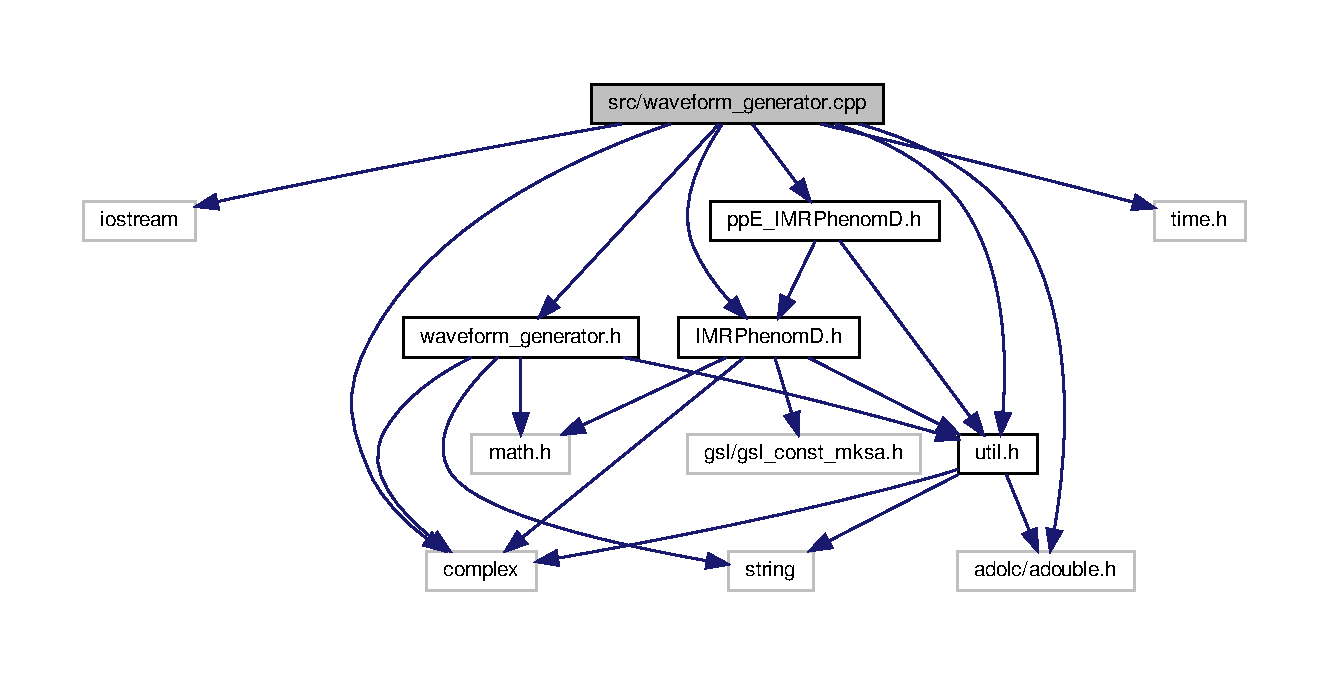
\includegraphics[width=350pt]{waveform__generator_8cpp__incl}
\end{center}
\end{figure}
\doxysubsection*{Functions}
\begin{DoxyCompactItemize}
\item 
{\footnotesize template$<$class T $>$ }\\int \mbox{\hyperlink{waveform__generator_8cpp_a8591c44df6b24c56f9cf6778eaaff211}{fourier\+\_\+waveform}} (T $\ast$frequencies, int length, std\+::complex$<$ T $>$ $\ast$waveform\+\_\+plus, std\+::complex$<$ T $>$ $\ast$waveform\+\_\+cross, string generation\+\_\+method, \mbox{\hyperlink{classgen__params__base}{gen\+\_\+params\+\_\+base}}$<$ T $>$ $\ast$parameters)
\begin{DoxyCompactList}\small\item\em Function to produce the plus/cross polarizations of an quasi-\/circular binary. \end{DoxyCompactList}\item 
int \mbox{\hyperlink{waveform__generator_8cpp_ae1722eb2df95b1de6495650b9e5ff630}{fourier\+\_\+waveform}} (double $\ast$frequencies, int length, double $\ast$waveform\+\_\+plus\+\_\+real, double $\ast$waveform\+\_\+plus\+\_\+imag, double $\ast$waveform\+\_\+cross\+\_\+real, double $\ast$waveform\+\_\+cross\+\_\+imag, string generation\+\_\+method, \mbox{\hyperlink{classgen__params}{gen\+\_\+params}} $\ast$parameters)
\item 
int \mbox{\hyperlink{waveform__generator_8cpp_a290382872adb5860aa7ba5f2c90a14af}{fourier\+\_\+waveform}} (double $\ast$frequencies, int length, std\+::complex$<$ double $>$ $\ast$waveform, string generation\+\_\+method, \mbox{\hyperlink{classgen__params}{gen\+\_\+params}} $\ast$parameters)
\begin{DoxyCompactList}\small\item\em Function to produce the (2,2) mode of an quasi-\/circular binary. \end{DoxyCompactList}\item 
int \mbox{\hyperlink{waveform__generator_8cpp_a0784e75fc03593f717553a5983aca394}{fourier\+\_\+waveform}} (double $\ast$frequencies, int length, double $\ast$waveform\+\_\+real, double $\ast$waveform\+\_\+imag, string generation\+\_\+method, \mbox{\hyperlink{classgen__params}{gen\+\_\+params}} $\ast$parameters)
\item 
{\footnotesize template$<$class T $>$ }\\int \mbox{\hyperlink{waveform__generator_8cpp_acbc169a17e10956bcc7e1e47fc3c0310}{fourier\+\_\+amplitude}} (T $\ast$frequencies, int length, T $\ast$amplitude, string generation\+\_\+method, \mbox{\hyperlink{classgen__params__base}{gen\+\_\+params\+\_\+base}}$<$ T $>$ $\ast$parameters)
\begin{DoxyCompactList}\small\item\em Function to produce the amplitude of the (2,2) mode of an quasi-\/circular binary. \end{DoxyCompactList}\item 
\mbox{\Hypertarget{waveform__generator_8cpp_aacebe5c329697d0c9f8ef3a0dbf351b4}\label{waveform__generator_8cpp_aacebe5c329697d0c9f8ef3a0dbf351b4}} 
template int {\bfseries fourier\+\_\+amplitude$<$ double $>$} (double $\ast$, int, double $\ast$, std\+::string, \mbox{\hyperlink{classgen__params__base}{gen\+\_\+params\+\_\+base}}$<$ double $>$ $\ast$)
\item 
\mbox{\Hypertarget{waveform__generator_8cpp_ad5faa8c46ea3876ad16b5c80d8b8ae53}\label{waveform__generator_8cpp_ad5faa8c46ea3876ad16b5c80d8b8ae53}} 
template int {\bfseries fourier\+\_\+amplitude$<$ adouble $>$} (adouble $\ast$, int, adouble $\ast$, std\+::string, \mbox{\hyperlink{classgen__params__base}{gen\+\_\+params\+\_\+base}}$<$ adouble $>$ $\ast$)
\item 
{\footnotesize template$<$class T $>$ }\\int \mbox{\hyperlink{waveform__generator_8cpp_a12a44f307fdb1bc05115b84c52f2e88c}{fourier\+\_\+phase}} (T $\ast$frequencies, int length, T $\ast$phase, string generation\+\_\+method, \mbox{\hyperlink{classgen__params__base}{gen\+\_\+params\+\_\+base}}$<$ T $>$ $\ast$parameters)
\begin{DoxyCompactList}\small\item\em Function to produce the phase of the (2,2) mode of an quasi-\/circular binary. \end{DoxyCompactList}\item 
\mbox{\Hypertarget{waveform__generator_8cpp_a53c29cfd7c4887ca3de425149eb38aa1}\label{waveform__generator_8cpp_a53c29cfd7c4887ca3de425149eb38aa1}} 
template int {\bfseries fourier\+\_\+phase$<$ double $>$} (double $\ast$, int, double $\ast$, std\+::string, \mbox{\hyperlink{classgen__params__base}{gen\+\_\+params\+\_\+base}}$<$ double $>$ $\ast$)
\item 
\mbox{\Hypertarget{waveform__generator_8cpp_abd8a9e9f681e02dbc3b8042401de2c4b}\label{waveform__generator_8cpp_abd8a9e9f681e02dbc3b8042401de2c4b}} 
template int {\bfseries fourier\+\_\+phase$<$ adouble $>$} (adouble $\ast$, int, adouble $\ast$, std\+::string, \mbox{\hyperlink{classgen__params__base}{gen\+\_\+params\+\_\+base}}$<$ adouble $>$ $\ast$)
\item 
{\footnotesize template$<$class T $>$ }\\int \mbox{\hyperlink{waveform__generator_8cpp_a5c1e4c24cb332e1a692502e4f3004eb5}{fourier\+\_\+phase}} (T $\ast$frequencies, int length, T $\ast$phase\+\_\+plus, T $\ast$phase\+\_\+cross, string generation\+\_\+method, \mbox{\hyperlink{classgen__params__base}{gen\+\_\+params\+\_\+base}}$<$ T $>$ $\ast$parameters)
\begin{DoxyCompactList}\small\item\em Function to produce the phase of the plus and cross mode of a quasi-\/circular binary. \end{DoxyCompactList}\item 
\mbox{\Hypertarget{waveform__generator_8cpp_ae6eee2f88bd28d69d60714919e9e40e3}\label{waveform__generator_8cpp_ae6eee2f88bd28d69d60714919e9e40e3}} 
template int {\bfseries fourier\+\_\+waveform$<$ double $>$} (double $\ast$, int, std\+::complex$<$ double $>$ $\ast$, std\+::complex$<$ double $>$ $\ast$, std\+::string, \mbox{\hyperlink{classgen__params__base}{gen\+\_\+params\+\_\+base}}$<$ double $>$ $\ast$)
\item 
\mbox{\Hypertarget{waveform__generator_8cpp_afd8d50ad1b6bb0e3d371debf50877f94}\label{waveform__generator_8cpp_afd8d50ad1b6bb0e3d371debf50877f94}} 
template int {\bfseries fourier\+\_\+waveform$<$ adouble $>$} (adouble $\ast$, int, std\+::complex$<$ adouble $>$ $\ast$, std\+::complex$<$ adouble $>$ $\ast$, std\+::string, \mbox{\hyperlink{classgen__params__base}{gen\+\_\+params\+\_\+base}}$<$ adouble $>$ $\ast$)
\item 
\mbox{\Hypertarget{waveform__generator_8cpp_a1f97fafbad6ad4527ae1447a19746bdf}\label{waveform__generator_8cpp_a1f97fafbad6ad4527ae1447a19746bdf}} 
template int {\bfseries fourier\+\_\+phase$<$ double $>$} (double $\ast$, int, double $\ast$, double $\ast$, std\+::string, \mbox{\hyperlink{classgen__params__base}{gen\+\_\+params\+\_\+base}}$<$ double $>$ $\ast$)
\item 
\mbox{\Hypertarget{waveform__generator_8cpp_a0c9227be02abd9079abb29bb86076d0b}\label{waveform__generator_8cpp_a0c9227be02abd9079abb29bb86076d0b}} 
template int {\bfseries fourier\+\_\+phase$<$ adouble $>$} (adouble $\ast$, int, adouble $\ast$, adouble $\ast$, std\+::string, \mbox{\hyperlink{classgen__params__base}{gen\+\_\+params\+\_\+base}}$<$ adouble $>$ $\ast$)
\end{DoxyCompactItemize}


\doxysubsection{Detailed Description}
File that handles the construction of the (2,2) waveform as described by \mbox{\hyperlink{classIMRPhenomD}{I\+M\+R\+PhenomD}} by Khan et. al.

Builds a waveform for given D\+E\+T\+E\+C\+T\+OR F\+R\+A\+ME parameters 

\doxysubsection{Function Documentation}
\mbox{\Hypertarget{waveform__generator_8cpp_acbc169a17e10956bcc7e1e47fc3c0310}\label{waveform__generator_8cpp_acbc169a17e10956bcc7e1e47fc3c0310}} 
\index{waveform\_generator.cpp@{waveform\_generator.cpp}!fourier\_amplitude@{fourier\_amplitude}}
\index{fourier\_amplitude@{fourier\_amplitude}!waveform\_generator.cpp@{waveform\_generator.cpp}}
\doxysubsubsection{\texorpdfstring{fourier\_amplitude()}{fourier\_amplitude()}}
{\footnotesize\ttfamily template$<$class T $>$ \\
int fourier\+\_\+amplitude (\begin{DoxyParamCaption}\item[{T $\ast$}]{frequencies,  }\item[{int}]{length,  }\item[{T $\ast$}]{amplitude,  }\item[{string}]{generation\+\_\+method,  }\item[{\mbox{\hyperlink{classgen__params__base}{gen\+\_\+params\+\_\+base}}$<$ T $>$ $\ast$}]{parameters }\end{DoxyParamCaption})}



Function to produce the amplitude of the (2,2) mode of an quasi-\/circular binary. 

By using the structure parameter, the function is allowed to be more flexible in using different method of waveform generation -\/ not all methods use the same parameters 
\begin{DoxyParams}{Parameters}
{\em frequencies} & double array of frequencies for the waveform to be evaluated at \\
\hline
{\em length} & integer length of all the arrays \\
\hline
{\em amplitude} & output array for the amplitude \\
\hline
{\em generation\+\_\+method} & String that corresponds to the generation method -\/ M\+U\+ST BE S\+P\+E\+L\+L\+ED E\+X\+A\+C\+T\+LY \\
\hline
\end{DoxyParams}
\mbox{\Hypertarget{waveform__generator_8cpp_a12a44f307fdb1bc05115b84c52f2e88c}\label{waveform__generator_8cpp_a12a44f307fdb1bc05115b84c52f2e88c}} 
\index{waveform\_generator.cpp@{waveform\_generator.cpp}!fourier\_phase@{fourier\_phase}}
\index{fourier\_phase@{fourier\_phase}!waveform\_generator.cpp@{waveform\_generator.cpp}}
\doxysubsubsection{\texorpdfstring{fourier\_phase()}{fourier\_phase()}\hspace{0.1cm}{\footnotesize\ttfamily [1/2]}}
{\footnotesize\ttfamily template$<$class T $>$ \\
int fourier\+\_\+phase (\begin{DoxyParamCaption}\item[{T $\ast$}]{frequencies,  }\item[{int}]{length,  }\item[{T $\ast$}]{phase,  }\item[{string}]{generation\+\_\+method,  }\item[{\mbox{\hyperlink{classgen__params__base}{gen\+\_\+params\+\_\+base}}$<$ T $>$ $\ast$}]{parameters }\end{DoxyParamCaption})}



Function to produce the phase of the (2,2) mode of an quasi-\/circular binary. 

By using the structure parameter, the function is allowed to be more flexible in using different method of waveform generation -\/ not all methods use the same parameters 
\begin{DoxyParams}{Parameters}
{\em frequencies} & double array of frequencies for the waveform to be evaluated at \\
\hline
{\em length} & integer length of all the arrays \\
\hline
{\em phase} & output array for the phase \\
\hline
{\em generation\+\_\+method} & String that corresponds to the generation method -\/ M\+U\+ST BE S\+P\+E\+L\+L\+ED E\+X\+A\+C\+T\+LY \\
\hline
\end{DoxyParams}
\mbox{\Hypertarget{waveform__generator_8cpp_a5c1e4c24cb332e1a692502e4f3004eb5}\label{waveform__generator_8cpp_a5c1e4c24cb332e1a692502e4f3004eb5}} 
\index{waveform\_generator.cpp@{waveform\_generator.cpp}!fourier\_phase@{fourier\_phase}}
\index{fourier\_phase@{fourier\_phase}!waveform\_generator.cpp@{waveform\_generator.cpp}}
\doxysubsubsection{\texorpdfstring{fourier\_phase()}{fourier\_phase()}\hspace{0.1cm}{\footnotesize\ttfamily [2/2]}}
{\footnotesize\ttfamily template$<$class T $>$ \\
int fourier\+\_\+phase (\begin{DoxyParamCaption}\item[{T $\ast$}]{frequencies,  }\item[{int}]{length,  }\item[{T $\ast$}]{phase\+\_\+plus,  }\item[{T $\ast$}]{phase\+\_\+cross,  }\item[{string}]{generation\+\_\+method,  }\item[{\mbox{\hyperlink{classgen__params__base}{gen\+\_\+params\+\_\+base}}$<$ T $>$ $\ast$}]{parameters }\end{DoxyParamCaption})}



Function to produce the phase of the plus and cross mode of a quasi-\/circular binary. 

By using the structure parameter, the function is allowed to be more flexible in using different method of waveform generation -\/ not all methods use the same parameters 
\begin{DoxyParams}{Parameters}
{\em frequencies} & double array of frequencies for the waveform to be evaluated at \\
\hline
{\em length} & integer length of all the arrays \\
\hline
{\em phase\+\_\+plus} & output array for the phase \\
\hline
{\em phase\+\_\+cross} & output array for the phase \\
\hline
{\em generation\+\_\+method} & String that corresponds to the generation method -\/ M\+U\+ST BE S\+P\+E\+L\+L\+ED E\+X\+A\+C\+T\+LY \\
\hline
\end{DoxyParams}
\mbox{\Hypertarget{waveform__generator_8cpp_ae1722eb2df95b1de6495650b9e5ff630}\label{waveform__generator_8cpp_ae1722eb2df95b1de6495650b9e5ff630}} 
\index{waveform\_generator.cpp@{waveform\_generator.cpp}!fourier\_waveform@{fourier\_waveform}}
\index{fourier\_waveform@{fourier\_waveform}!waveform\_generator.cpp@{waveform\_generator.cpp}}
\doxysubsubsection{\texorpdfstring{fourier\_waveform()}{fourier\_waveform()}\hspace{0.1cm}{\footnotesize\ttfamily [1/4]}}
{\footnotesize\ttfamily int fourier\+\_\+waveform (\begin{DoxyParamCaption}\item[{double $\ast$}]{frequencies,  }\item[{int}]{length,  }\item[{double $\ast$}]{waveform\+\_\+plus\+\_\+real,  }\item[{double $\ast$}]{waveform\+\_\+plus\+\_\+imag,  }\item[{double $\ast$}]{waveform\+\_\+cross\+\_\+real,  }\item[{double $\ast$}]{waveform\+\_\+cross\+\_\+imag,  }\item[{string}]{generation\+\_\+method,  }\item[{\mbox{\hyperlink{classgen__params}{gen\+\_\+params}} $\ast$}]{parameters }\end{DoxyParamCaption})}


\begin{DoxyParams}{Parameters}
{\em frequencies} & double array of frequencies for the waveform to be evaluated at \\
\hline
{\em length} & integer length of all the arrays \\
\hline
{\em waveform\+\_\+plus\+\_\+real} & complex array for the output waveform \\
\hline
{\em waveform\+\_\+plus\+\_\+imag} & complex array for the output waveform \\
\hline
{\em waveform\+\_\+cross\+\_\+real} & complex array for the output waveform \\
\hline
{\em waveform\+\_\+cross\+\_\+imag} & complex array for the output waveform \\
\hline
{\em generation\+\_\+method} & String that corresponds to the generation method -\/ M\+U\+ST BE S\+P\+E\+L\+L\+ED E\+X\+A\+C\+T\+LY \\
\hline
{\em parameters} & structure containing all the source parameters \\
\hline
\end{DoxyParams}
\mbox{\Hypertarget{waveform__generator_8cpp_a0784e75fc03593f717553a5983aca394}\label{waveform__generator_8cpp_a0784e75fc03593f717553a5983aca394}} 
\index{waveform\_generator.cpp@{waveform\_generator.cpp}!fourier\_waveform@{fourier\_waveform}}
\index{fourier\_waveform@{fourier\_waveform}!waveform\_generator.cpp@{waveform\_generator.cpp}}
\doxysubsubsection{\texorpdfstring{fourier\_waveform()}{fourier\_waveform()}\hspace{0.1cm}{\footnotesize\ttfamily [2/4]}}
{\footnotesize\ttfamily int fourier\+\_\+waveform (\begin{DoxyParamCaption}\item[{double $\ast$}]{frequencies,  }\item[{int}]{length,  }\item[{double $\ast$}]{waveform\+\_\+real,  }\item[{double $\ast$}]{waveform\+\_\+imag,  }\item[{string}]{generation\+\_\+method,  }\item[{\mbox{\hyperlink{classgen__params}{gen\+\_\+params}} $\ast$}]{parameters }\end{DoxyParamCaption})}


\begin{DoxyParams}{Parameters}
{\em frequencies} & double array of frequencies for the waveform to be evaluated at \\
\hline
{\em length} & integer length of all the arrays \\
\hline
{\em waveform\+\_\+real} & complex array for the output waveform \\
\hline
{\em waveform\+\_\+imag} & complex array for the output waveform \\
\hline
{\em generation\+\_\+method} & String that corresponds to the generation method -\/ M\+U\+ST BE S\+P\+E\+L\+L\+ED E\+X\+A\+C\+T\+LY \\
\hline
{\em parameters} & structure containing all the source parameters \\
\hline
\end{DoxyParams}
\mbox{\Hypertarget{waveform__generator_8cpp_a290382872adb5860aa7ba5f2c90a14af}\label{waveform__generator_8cpp_a290382872adb5860aa7ba5f2c90a14af}} 
\index{waveform\_generator.cpp@{waveform\_generator.cpp}!fourier\_waveform@{fourier\_waveform}}
\index{fourier\_waveform@{fourier\_waveform}!waveform\_generator.cpp@{waveform\_generator.cpp}}
\doxysubsubsection{\texorpdfstring{fourier\_waveform()}{fourier\_waveform()}\hspace{0.1cm}{\footnotesize\ttfamily [3/4]}}
{\footnotesize\ttfamily int fourier\+\_\+waveform (\begin{DoxyParamCaption}\item[{double $\ast$}]{frequencies,  }\item[{int}]{length,  }\item[{std\+::complex$<$ double $>$ $\ast$}]{waveform,  }\item[{string}]{generation\+\_\+method,  }\item[{\mbox{\hyperlink{classgen__params}{gen\+\_\+params}} $\ast$}]{parameters }\end{DoxyParamCaption})}



Function to produce the (2,2) mode of an quasi-\/circular binary. 

By using the structure parameter, the function is allowed to be more flexible in using different method of waveform generation -\/ not all methods use the same parameters 
\begin{DoxyParams}{Parameters}
{\em frequencies} & double array of frequencies for the waveform to be evaluated at \\
\hline
{\em length} & integer length of all the arrays \\
\hline
{\em waveform} & complex array for the output waveform \\
\hline
{\em generation\+\_\+method} & String that corresponds to the generation method -\/ M\+U\+ST BE S\+P\+E\+L\+L\+ED E\+X\+A\+C\+T\+LY \\
\hline
{\em parameters} & structure containing all the source parameters \\
\hline
\end{DoxyParams}
\mbox{\Hypertarget{waveform__generator_8cpp_a8591c44df6b24c56f9cf6778eaaff211}\label{waveform__generator_8cpp_a8591c44df6b24c56f9cf6778eaaff211}} 
\index{waveform\_generator.cpp@{waveform\_generator.cpp}!fourier\_waveform@{fourier\_waveform}}
\index{fourier\_waveform@{fourier\_waveform}!waveform\_generator.cpp@{waveform\_generator.cpp}}
\doxysubsubsection{\texorpdfstring{fourier\_waveform()}{fourier\_waveform()}\hspace{0.1cm}{\footnotesize\ttfamily [4/4]}}
{\footnotesize\ttfamily template$<$class T $>$ \\
int fourier\+\_\+waveform (\begin{DoxyParamCaption}\item[{T $\ast$}]{frequencies,  }\item[{int}]{length,  }\item[{std\+::complex$<$ T $>$ $\ast$}]{waveform\+\_\+plus,  }\item[{std\+::complex$<$ T $>$ $\ast$}]{waveform\+\_\+cross,  }\item[{string}]{generation\+\_\+method,  }\item[{\mbox{\hyperlink{classgen__params__base}{gen\+\_\+params\+\_\+base}}$<$ T $>$ $\ast$}]{parameters }\end{DoxyParamCaption})}



Function to produce the plus/cross polarizations of an quasi-\/circular binary. 

By using the structure parameter, the function is allowed to be more flexible in using different method of waveform generation -\/ not all methods use the same parameters

This puts the responsibility on the user to pass the necessary parameters

{\itshape N\+E\+ED TO O\+U\+T\+L\+I\+NE O\+P\+T\+I\+O\+NS F\+OR E\+A\+CH M\+E\+T\+H\+OD IN D\+E\+P\+TH}

N\+EW P\+H\+A\+SE O\+P\+T\+I\+O\+NS for

P\+H\+E\+N\+O\+MD O\+N\+LY\+:

If phic is assigned, the reference frequency and reference phase are I\+G\+N\+O\+R\+ED.

If Phic is unassigned, a reference phase A\+ND a reference frequency are looked for.\+If no options are found, both are set to 0.

If tc is assigned, it is used.

If tc is unassigned, the waveform is shifted so the merger happens at 0.

Phenom\+Pv2\+:

Phi\+Ref and f\+\_\+ref are required, phic is not an option.

tc, if specified, is used with the use of interpolation. If not, tc is set such that coalescence happens at t=0 
\begin{DoxyParams}[1]{Parameters}
 & {\em frequencies} & double array of frequencies for the waveform to be evaluated at \\
\hline
 & {\em length} & integer length of all the arrays \\
\hline
\mbox{\texttt{ out}}  & {\em waveform\+\_\+plus} & complex array for the output plus polarization waveform \\
\hline
\mbox{\texttt{ out}}  & {\em waveform\+\_\+cross} & complex array for the output cross polarization waveform \\
\hline
 & {\em generation\+\_\+method} & String that corresponds to the generation method -\/ M\+U\+ST BE S\+P\+E\+L\+L\+ED E\+X\+A\+C\+T\+LY \\
\hline
 & {\em parameters} & structure containing all the source parameters \\
\hline
\end{DoxyParams}

%--- End generated contents ---

% Index
\backmatter
\newpage
\phantomsection
\clearemptydoublepage
\addcontentsline{toc}{chapter}{Index}
\printindex

\end{document}
